\documentclass{report}

%%% Работа с языком
%\usepackage{cmap}					    % поиск в PDF				    % русские буквы в формулах
\usepackage[T2A]{fontenc}			% кодировка
\usepackage[utf8]{inputenc}             % кодировка исходного текста
\usepackage[english,ukrainian]{babel}	% локализация и переносы	    
\usepackage{indentfirst}

\usepackage[a4paper, top=25mm, bottom=25mm, left=30mm, right=30mm]{geometry}

\usepackage{amsmath,amsfonts,amssymb,amsthm,mathtools} % AMS

\usepackage{makecell}% Прикольная настройка ячеек в tabular 
%http://ctan.math.utah.edu/ctan/tex-archive/macros/latex/contrib/makecell/makecell-rus.pdf

\usepackage{diagbox}
% Разделение клеток tabular по диагонали

\usepackage{multicol} % Несколько колонок
\usepackage{wrapfig} % Картинки посреди текста
\usepackage{chngcntr} % для нумерации формул
\usepackage{enumitem} % чтоб можно было делать римскую нумерацию
\usepackage{mdwlist}
\usepackage{adjustbox}
\usepackage[psdextra]{hyperref}
\hypersetup{unicode=true}
\hypersetup{
    colorlinks=true,
    linkcolor=blue,
}
\setlist[enumerate]{nosep}

%%%% Теоремы, определения и т.д. и т.п.
\theoremstyle{plain} % Это стиль по умолчанию, его можно не переопределять.
\newtheorem{theorem}{Теорема}
\newtheorem{proposition}{Твердження}
\renewcommand{\qedsymbol}{$\blacktriangle$}
 
\theoremstyle{definition} % "Определение"
\newtheorem{definition}{Означення}[section]
\newtheorem*{definition*}{Означення}
\newtheorem*{example}{Приклад}

\theoremstyle{remark}
\newtheorem*{remark}{Зауваження}
\newtheorem*{exercise}{Вправа}

\counterwithout{equation}{chapter} % нумерация формул
\counterwithin*{equation}{section}

%%%% Картинки
\usepackage{graphicx}
\usepackage{tikz}
\usepackage{pgfplots}
\pgfplotsset{compat=1.17}

\usetikzlibrary{patterns}
\usetikzlibrary{shapes.geometric}
\usetikzlibrary{arrows.meta}
\usetikzlibrary{shapes.geometric}
\graphicspath{{pictures/}}
\DeclareGraphicsExtensions{.pdf,.png,.jpg}


\author{\Huge Каніовська І.Ю.}
\title{
    \textbf{\fontsize{40}{48}\selectfont Конспект лекцій \\з теорії ймовірностей \\та математичної \\\vspace{0.64em}статистики}
    }
\date{}

\begin{document} 
    \maketitle
    \setcounter{page}{2}
    \tableofcontents
    \part{Теорія ймовірностей}
    \chapter{Випадкові події}
        % !TEX root = ../main.tex

\section{Основні поняття теорії ймовірностей}
\subsection{Теоретико-множинний підхід до основних понять ТЙ}
\begin{definition}
    \emph{Стохастичним експериментом (випробуванням)} називається експеримент, 
    який можна повторювати неодноразово, зберігаючи певні умови, і результат якого 
    експерименту заздалегідь передбачити неможливо.
\end{definition}
\begin{definition}
    Будь-який результат СЕ називається \emph{подією}.
\end{definition}
\begin{example}
    \begin{enumerate}
        \item СЕ --- кидання кубика один раз, подія --- випало 6 очок.
        \item СЕ --- кидання кубика двічі, подія --- сума очок, що випала, дорівнює 6.
    \end{enumerate}
\end{example}

\noindent \textbf{Події бувають:}
\begin{enumerate}
    \item Випадкові --- можуть відбутися чи не відбутися при проведенні СЕ.
    \item Неможливі --- ніколи не відбуваються в даному СЕ.
    \item Вірогідні --- завжди відбуваються в даному СЕ.
\end{enumerate}

Будемо вважати, що кожному СЕ можна поставити у відповідність деяку множину, що
називається \emph{простором елементарних подій} $\Omega$. 
Під \emph{елементарними подіями} $\omega$ будемо розуміти єдині
логічно можливі події СЕ, що виключають одна одну.
\begin{example}
    \begin{enumerate}
        \item СЕ --- кидання кубика один раз. 
        $\Omega = \left\{\omega_1, \omega_2, ..., \omega_6\right\}$, 
        де події 

        $\omega_k = \left\{\text{випало } k \text{ очок}\right\}, k = 1,...,6$.
        \item СЕ --- кидання монетки до першої появи герба.
        $\Omega = \left\{\omega_1, \omega_2, ..., \omega_k, ...\right\}$, 
        
        де $\omega_i = \left\{\text{герб випав на }i\text{-тому киданні}\right\}, i\in \mathbb{N}$.
        \item СЕ --- зустріч двох осіб, що домовилися зустрітися протягом години.
        $x$ --- час приходу першої особи, $y$ --- час приходу другої, $0\leq x, y \leq 1$.
        $\Omega = \left\{ \left( x, y\right): 0\leq x, y \leq 1\right\}\subset \mathbb{R}^2$.
    \end{enumerate}
\end{example}
В подальшому випадкові події позначатимемо $A, B, C, ...$. 
\emph{Випадкова подія --- підмножина $\Omega$}. 
У прикладі з киданням кубика один раз $A = \left\{\text{випало }6\text{ очок}\right\} = \left\{ \omega_6\right\}$.
В загальному випадку маємо $A = \left\{\omega_{k1}, \omega_{k2}, ..., \omega_{kn}, ...\right\} \subset \Omega$.
Неможлива подія --- $\varnothing$, вірогідна --- $\Omega$. 

\begin{remark}
    Розглядаємо події в межах фіксованих СЕ та простору елементарних подій.
\end{remark}
\begin{enumerate}
    \item \emph{Включення} $A \subset B$ означає, що якщо відбулася подія $A$, то обов'язково відбудеться подія $B$.
    Наприклад, $A = \left\{\text{витягнуто даму пік}\right\}, B = \left\{\text{витягнуто карту чорної масті}\right\}$. 
    Очевидно, $A\subset B$.

    Рівність подій: $\left( A \subset B, B \subset A \right) \iff \left( A = B\right)$.
    \item \emph{Об'єднання подій} $A \cup B$ --- це подія, яка відбувається тоді, коли відбувається
    принаймні одна з подій $A$ чи $B$.

    Властивості: $A \cup A = A$,  $A \cup B = B \cup A$, $\left( A \subset B \right) \Rightarrow \left( A \cup B = B \right)$, 
    $A \cup \Omega = \Omega$, $A \cup \varnothing = A$, $\left( A \cup B \right) \cup C = A \cup \left( B \cup C \right)$.

    Операція узагальнюється на скінченну або зліченну кількість подій: $A = \bigcup\limits_{i=1}^{n \left( \infty \right)} A_i$.
    \item \emph{Перетин подій} $A \cap B$ --- це подія, яка відбувається тоді, коли $A$ і $B$ відбуваються одночасно.

    Властивості: $A \cap A = A$,  $A \cap B = B \cap A$, $\left( A \subset B \right) \Rightarrow \left( A \cap B = A \right)$, 
    $A \cap \Omega = A$, $A \cap \varnothing = \varnothing$, $\left( A \cap B \right) \cap C = A \cap \left( B \cap C \right)$,
    $A \cap B \subset A$, $A \cap B \subset B$, $\left( A \cup B \right) \cap C = \left( A \cap C \right) \cup \left( B \cap C \right)$,
    $\left( A \cap B \right) \cup C = \left( A \cup C \right) \cap \left( B \cup C \right)$.

    Операція узагальнюється на скінченну або зліченну кількість подій: $A = \bigcap\limits_{i=1}^{n \left( \infty \right)} A_i$.
\end{enumerate}
\begin{definition}
    Події $A$ та $B$ називається \emph{несумісними}, якщо вони не відбуваються одночасно: $A \cap B = \varnothing$.
    Узагальнення: події $A_1, A_2, ..., A_n, ...$ називаються \emph{попарно несумісними}, якщо $A_i \cap A_j = \varnothing$ для $i \neq j$.
\end{definition}
\begin{definition}
    Події $A_1, A_2, ..., A_n, ...$ утворюють \emph{повну групу подій}, якщо вони попарно несумісні 
    та $\bigcup\limits_{i=1}^{n \left( \infty \right)} A_i = \Omega$.
\end{definition}
\begin{enumerate}
    \setcounter{enumi}{3}
    \item \emph{Протилежна подія} $\overline{A}$ --- це подія, яка відбувається тоді, коли $A$ не відбувається.
    
    Властивості: $A \cup \overline{A} = \Omega$, $A \cap \overline{A} = \varnothing$, $\overline{\left( A \cup B \right)} = \overline{A} \cap \overline{B}$,
    $\overline{\left( A \cap B \right)} = \overline{A} \cup \overline{B}$.
    \item \emph{Різниця подій} $A \backslash B$ --- це подія $A \cap \overline{B}$. Для протилежної події маємо $\overline{A} =  \Omega \backslash A$.
\end{enumerate}

\begin{definition}
    Непорожня система підмножин $\mathcal{F}$ простору елементарних подій $\Omega$ утворює \emph{алгебру подій}, якщо:
    \begin{enumerate}
        \item $\Omega \in \mathcal{F}$;
        \item $\left( A, B \in \mathcal{F}\right) \Rightarrow \left( A \cup B \in \mathcal{F}\right)$;
        \item $\left( A \in \mathcal{F}\right) \Rightarrow \left( \overline{A} \in \mathcal{F}\right)$.
    \end{enumerate}
    \emph{Узагальнення:} якщо $\Omega$ містить зліченну кількість подій, то означення $\sigma$-алгебра отримаємо заміною умови
    2 на $\left(\forall n \in \mathbb{N}: A_n \in \mathcal{F} \right) \Rightarrow \left( \bigcup\limits_{n=1}^{\infty} A_n \in \mathcal{F}\right)$.
    
    Пара $\left\{\Omega, \mathcal{F}\right\}$ називається \emph{вимірним простором стохастичного експерименту}.
\end{definition}

\subsection{Класична модель ймовірності}
Дослідника завжди цікавить кількісна характеристика появи тієї чи іншої події.

Нехай $\Omega$ --- скінченний чи зліченний. 
Поставимо у відповідність кожній елементарній події $\omega_k$ число $p_k\geq 0$ так, що $\sum\limits_{k=0}^{ n \left( \infty\right)}p_k = 1$.
Тоді $\P(A) = \sum\limits_{\omega_k \in A} p_k$ --- кількісна характеристика, ймовірність події $A$.

\begin{example}
    \emph{Класична модель ймовірності}. Якщо простір елементарних подій $\Omega$ СЕ скінченний
    та всі $\omega_k$ рівноможливі, то такий СЕ називається \emph{класичним}.
    В такому випадку $p_1 = p_2 = ... = p_n = \frac{1}{n}$, де $n = \mathrm{card}(\Omega)$.
    
    \begin{equation}\label{eq:m_n}
        \P(A) = \sum\limits_{\omega_k \in A} p_k = \frac{m}{n} = \frac{\text{кількість елементарних подій в } A}{\text{загальна кількість елементарних подій}}
    \end{equation}
\end{example}
Ймовірності, що розраховуються за формулою \eqref{eq:m_n}, називаються \emph{класичними}.
\begin{example}
    \begin{enumerate}
        \item <<Задачі про вибір>> --- коли з великої кількості чогось вибирають певну кількість.
        Наприклад, з урни з 10 кульками, 3 чорними та 7 білими, навмання витягають 5 кульок.
        Обчислимо ймовірність події $A = \left\{ \text{серед них 2 чорних кульки}\right\}$:
        $\P(A) = \frac{C_3^2\cdot C_7^3}{C_{10}^5} = \frac{3\cdot 35}{252} = \frac{5}{12}$.
        \item <<Задачі про ліфт>>. 5 осіб одночасно зайшли в ліфт 11-поверхового будинку. 
        Яка ймовірність того, що вони всі вийдуть на різних поверхах, починаючи з другого?
        
        $\P(A) = \frac{A_{10}^5}{\widetilde{A}_{10}^5} = \frac{10\cdot 9\cdot 8\cdot 7 \cdot 6}{10^5} = 0.3024$. 
        Тут $A_n^k$ та $\widetilde{A}_n^k$ --- кількості розміщень без повторень та з повтореннями відповідно.
    \end{enumerate}
\end{example}

\noindent \textbf{Властивості класичної ймовірності:}
\begin{enumerate}
    \item $\forall A \in \mathcal{F}: 0 \leq \P(A) \leq 1$.
    \item $\P(\Omega) = 1$.
    \item $\P(\overline{A}) = 1 - \P(A)$.
    \item $\P(\varnothing) = 0$.
    \item $\P(A\cup B) = \P(A) + \P(B) - \P(A\cap B)$, для несумісних $A$ і $B$ $\P(A\cup B) = \P(A) + \P(B)$.
    \item $\left( A \subset B\right) \Rightarrow \left( \P(A) \leq \P(B)\right)$.
    \item Якщо $A_1, A_2, ..., A_n$ --- повна група подій СЕ, то $\P\left(\bigcup\limits_{i=1}^{n} A_i\right) = 1$.
\end{enumerate}

\subsection{Геометрична модель ймовірності}
\begin{example}
    Нехай точка кидається навмання на відрізок $\left[a; b\right]$. 
    Яка ймовірність її 
    потрапляння в $\left<\alpha; \beta\right> \subset  \left[a; b\right]$?
    Розглянемо подію $A = \left\{ 
        \text{точка потрапила в} \left<\alpha; \beta\right>
    \right\}$.
    \newline
    \hbox to \hsize{\hfil{
        \begin{tikzpicture}
            \draw [fill] (0, 0) circle [radius = 0.05];
            \node [below] at (0, 0) {$a$};
            \node [above] at (0, 0) { };
            \node [below] at (8, 0) {$b$};
            \draw [-{Straight Barb}] (6,0) to (2,0) {};
            \draw [-{Straight Barb}] (2,0) to (6,0) {};
            \node [below] at (2, 0) {$\alpha$};
            \node [below] at (6, 0) {$\beta$};
            \draw [fill] (8, 0) circle [radius = 0.05];
            \draw [thick] (0, 0) -- (8, 0);
        \end{tikzpicture}
    }\hfil}
    Логічно припустити, що $\P(A) = k\cdot l_{\left<\alpha; \beta\right>}$ для деякого $k > 0$.
    Тоді $\P(\Omega) = 1 = k\cdot l_{\left[a; b\right]}$. Таким чином, 
    $k = \frac{1}{l_{\left[a; b\right]}} = \frac{1}{b-a}$,
    тому $\P(A) = \frac{l_{\left<\alpha; \beta\right>}}{l_{\left[a; b\right]}}$.
\end{example}
Нехай простір елементарних подій інтерпретується як замкнена область в 
$ \mathbb{R} ^n$, а випадкові події --- її підмножини. В якості $\sigma$-алгебри 
подій $\mathcal{F}$ беремо підмножини, що мають міру $\mu$. Тоді в якості ймовірності 
деякої події $A$ беремо $\P(A) = \frac{\mu(A)}{\mu(\Omega)}$. 
Наприклад, в $\mathbb{R}^1$ беремо міру <<довжина>>, в $\mathbb{R}^2$ --- <<площа>>, а в $\mathbb{R}^3$ --- <<об'єм>>.

Ймовірності, що знаходяться таким чином називаються \emph{геометричними}, а сама модель 
називається \emph{геометричною моделлю ймовірності}.
Геометрична модель може використовуватись, 
коли $\Omega$ має геометричну інтерпретацію як замкнена область в $\mathbb{R}^n$,
а елементарні події --- рівноможливі.

\begin{example}[задача Бюффона]\label{buffon}
    На площині накреслені паралельні прямі на відстані $2a$, на них кидається 
    голка довжиною $2l,\; l \leq a $. Яка ймовірність того, що голка перетне 
    яку-небудь пряму?
    \newline
    \hbox to \hsize{\hfil{
        \begin{tikzpicture}[scale = 0.5]
            \draw [thick] (0, 0) -- (8, 0);
            \draw [thick] (0, 2) -- (8, 2);
            \draw [thick] (0, 4) -- (8, 4);
            \draw [thick] (0, 6) -- (8, 6);
            \draw [{Straight Barb}-{Straight Barb}] (7.5,4) to (7.5,6);
            \node [right] at (7.5, 5) {$2a$}; 
        \end{tikzpicture}
        \begin{tikzpicture}[scale = 1]
            \draw (0, 0) -- (4, 0);
            \draw (0, 2) -- (4, 2);
            \draw [thick] (0.5, -0.5)-- (2.5, 1.5);
            \draw [{Straight Barb}-{Straight Barb}] (3.5,0) to (3.5,2);
            \draw [{Straight Barb}-{Straight Barb}] (1.5,0) to (1.5,0.5);
            \node [right] at (3.5, 1) {$2a$};
            \node [right] at (1.5, 0.25) {$ x $};
            \draw [-{Straight Barb}](2.5, 0) to [out = 90, in = 0](1.75, 0.75);
            \node [right] at (2.28, 0.53) {$ \varphi $};
        \end{tikzpicture}
    }\hfil}
    Достатньо розглядати лише дві прямі. $\Omega = \left\{(\varphi, x)\in 
    \mathbb{R}^2: \varphi \in \left[0; \pi\right], x \in \left[0; a\right] 
    \right\}$
    \newline
    При такій побудові простору елементарних подій подія $A = \left\{\text{голка 
    перетне пряму}\right\} =$
    \newline
    $\left\{(\varphi, x)\in 
    \Omega: x\leq l\sin\varphi\right\}$
    \newline
    \hbox to \hsize{\hfil{
        \begin{tikzpicture}
            \draw [<->] (4, 0) -- (0, 0) -- (0, 2.5);
            \node [left] at (0, 2.5) {$x$};
            \node [below] at (4, 0) {$\varphi$};
            \draw [domain=0:pi,fill=gray] plot (\x, {1*sin(\x r)});
            \node [below] at (0, 0) {$0$};
            \node [below] at (pi, 0) {$\pi$};
            \draw [dashed] (0,1) to (pi/2,1);
            \node [left] at (0, 1) {$l$};
            \draw (0,2) -- (pi, 2) -- (pi, 0);
            \node [left] at (0, 2) {$a$};
            \node [below left] at (pi, 2) {$\Omega$};
            \node [above] at (pi/2, 0.25) {$A$};
        \end{tikzpicture}
    }\hfil}
    $\P(A) = \frac{S(A)}{S(\Omega)},\; S(\Omega) = \pi a,\;S(A) = \int\limits_0^\pi 
    l\sin\varphi\ d\varphi = l\left.(-\cos\varphi)\right|^\pi_0 = 2l$.
    Отже, $\P(A) = \frac{2l}{\pi a}$.
    \newline
    Якщо провести $n$ кидань голки, у $m$ з яких голка потрапить на пряму, то за допомогою приблизної рівності $\frac{m}{n} 
    \approx \frac{2l}{\pi a}$ можна приблизно обчислити число $\pi$. 
    Наприклад, якщо взяти $n=5000, m=2532, l/a = 0.8$, то отримаємо $\pi \approx 3.1596$.
\end{example}
\begin{example}[парадокс Бертрана]
    Нехай в колі радіусом $R$ навмання обирається хорда. Яка ймовірність того, 
    що її довжина буде більшою за довжину сторони правильного трикутника, 
    вписаного в це коло?
    \newline
    Існують три способи розв'язання цієї задачі, причому кожен з них дає різний результат.
    
    \textbf{Спосіб 1.}
    З міркувань симетрії обирається якийсь фіксований діаметр кола і розглядається
    всі перпендикулярні до нього хорди. Серед них і обирається навмання довільна хорда.
    Очевидно, що кожна хорда у цьому випадку може бути однозначно визначена своєю серединою,
    тобто кожній хорді можна взаємно однозначно поставити у відповідність координату її середини,
    якщо за початок відліку взяти якийсь з кінців фіксованого діаметру.
    \newline
    \hbox to \hsize{\hfil{
        \begin{tikzpicture}[scale = 1.5]
            \draw (0, 0) circle [radius = 1]; 
            \draw (0, 1) -- (-0.86602540378, -0.5); 
            \draw (0, 1) -- (0.86602540378, -0.5);
            \draw (0.86602540378, -0.5) -- (-0.86602540378, -0.5);
            \draw [->] (-1,0) to (1, 0);
            \node [left] at (-1, 0) {$0$};
            \node [right] at (1, 0) {$2R$};
            \draw [dashed] (0, -1) to (0, 1);
            \draw [dashed] (-0.3, -0.954) to (-0.3, 0.954);
            \draw [dashed] (-0.7, -0.714) to (-0.7, 0.714);
            \draw [dashed] (0.3, -0.954) to (0.3, 0.954);
            \draw [dashed] (0.7, -0.714) to (0.7, 0.714);
            \draw [ultra thick] (-0.5, 0) -- (0.5, 0);
            \draw [ultra thick] (-0.5, 0.05) -- (-0.5, -0.05);
            \draw [ultra thick] (0.5, 0.05) -- (0.5, -0.05);
            \node [below] at (-0.5, 0) {$\frac{R}{2}$};
            \node [below] at (0.5, 0) {$\frac{3R}{2}$};
        \end{tikzpicture}
    }\hfil}
    Таким чином, множина всіх значень координати середини хорди $\Omega = \left[0; 2R\right]$. 
    Множина, що відповідає події --- це відрізок $A = \left[\frac{R}{2}; \frac{3R}{2}\right]$.
    В якості міри візьмемо довжину. Тоді $\P(A) = \frac{l(A)}{l(\Omega)} = \frac{R}{2R}= \frac{1}{2}$.
    
    \textbf{Спосіб 2.}
    В цьому способі пропонується розглядати тільки хорди з одним закріпленим кінцем.
    Кожній хорді поставимо у відповідність ту частину дуги кола, яка потрапляє у кут $\varphi$,
    що утворює хорда з дотичною, проведеною через точку закріплення кінця всіх хорд.
    \newline
    \hbox to \hsize{\hfil{
        \begin{tikzpicture}[scale = 1.5]
            \draw (0, 0) circle [radius = 1];
            \draw (0, 1) -- (-0.86602540378, -0.5); 
            \draw (0, 1) -- (0.86602540378, -0.5);
            \draw (0.86602540378, -0.5) -- (-0.86602540378, -0.5);
            \draw (-1.2, 1) -- (1.2, 1);
            \draw [fill] (0, 1) circle [radius = 0.05];
            \draw [fill] (0.17, -0.985) circle [radius = 0.05];
            \draw [fill] (1, 0) circle [radius = 0.05];
            \draw [fill] (-0.967, -0.256) circle [radius = 0.05];
            \draw (0.16, 1) arc (0:-46:0.16);
            \draw (0.19, 1) arc (0:-46:0.19);
            %\node [above] at (0, 1);
            \draw [dashed] (0, 1) to (0.17, -0.985);
            \draw [dashed] (0, 1) to (1, 0);
            \draw [dashed] (0, 1) to (-0.967, -0.256);
            \node [below right] at (0.14, 1) {$_\varphi$};
            \draw [ultra thick](0.86602540378, -0.5) to [out = 242, in = 0](0, -1);
            \draw [ultra thick](0, -1) to [out = 180, in = 300](-0.86602540378, -0.5);
        \end{tikzpicture}
    }\hfil}
    Тоді множина $\Omega = \left[ 0; \pi\right]$, а $A = \left[ \frac{\pi}{3}; \frac{2\pi}{3}\right]$.
    Знову візьмемо за міру довжину і отримаємо $\P(A) = \frac{\pi /3}{\pi} = \frac{1}{3}$.
    
    \textbf{Спосіб 3.}
    Розглядаються всі хорди кола. Кожній з них взаємно однозначно ставиться у відповідність точка її середини $(x,y)$,
    якщо за початок координат прийняти центр кола.
    \newline
    \hbox to \hsize{\hfil{
        \begin{tikzpicture}[scale = 1.8]
            \draw (0, 0) circle [radius = 1];
            \draw (0, 0) circle [radius = 0.5];
            \draw (0, 0) [fill] circle [radius = 0.05];
            \draw (0, 1) -- (-0.86602540378, -0.5); 
            \draw (0, 1) -- (0.86602540378, -0.5);
            \draw (0.86602540378, -0.5) -- (-0.86602540378, -0.5);
            \draw (-0.737, 0.675) [fill] circle [radius = 0.05];
            \draw (0.878, 0.479) [fill] circle [radius = 0.05];
            \draw [dashed] (-0.737, 0.675) to (0.878, 0.479);
            \draw [dashed] (0, 0) to (0.0705, 0.577);
            \draw (0.0705, 0.577) [fill] circle [radius = 0.05];
        \end{tikzpicture}
    }\hfil}
    В такому випадку $\Omega = \left\{ (x,y)\in \mathbb{R}^2: x^2 + y^2 \leq R^2\right\}$,
    а $A = \left\{ (x,y)\in \Omega: x^2 + y^2 \leq \frac{R^2}{4}\right\}$.
    Тоді $\P(A) = \frac{\pi R^2/4}{\pi R^2} = \frac{1}{4}$.

    Жозеф Бертран був противником геометричного означення ймовірності.
    Він казав, що воно не дає можливості однозначно обчислити ймовірність
    однієї і тієї ж випадкової події та використовував вищенаведений приклад
    для доведення своєї правоти. Дійсно, було отримано три різних відповіді при
    розв'язанні однієї задачі. Так в чому ж справа? Насправді, помилка полягає
    у різних трактуваннях поняття <<навмання обрана хорда>>.
    В кожному з трьох способів це трактування було різним, що й стало причиною різних відповідей.
\end{example}

        % !TEX root = ../main.tex

\newlength\Radius
\setlength\Radius{2cm}

\section{Аксіоми теорії ймовірностей}
Розглянуті ймовірнісні схеми (класична, геометрична) мають свої недоліки і не дають можливості описати різноманіття стохастичних експериментів.
Сучасна теорія ймовірностей побудована на основі аксіом, які були запропоновані академіком 
\href{https://uk.wikipedia.org/wiki/%D0%9A%D0%BE%D0%BB%D0%BC%D0%BE%D0%B3%D0%BE%D1%80%D0%BE%D0%B2_%D0%90%D0%BD%D0%B4%D1%80%D1%96%D0%B9_%D0%9C%D0%B8%D0%BA%D0%BE%D0%BB%D0%B0%D0%B9%D0%BE%D0%B2%D0%B8%D1%87}{Андрієм Миколайовичем Колмогоровим} у 1929 році.
Класична та геометрична схеми виявляються частинними випадками цього аксіоматичного підходу.

\subsection{Система аксіом Колмогорова}\index{система аксіом Колмогорова}
\begin{enumerate}[label=\Roman*.]
    \item Побудова вимірного простору $\left\{ \Omega, \mathcal{F}\right\}$:
    \begin{enumerate}[label = \textbf{A\arabic*:}]
        \item Будь-якому стохастичному експерименту можна поставити у відповідність
        простір елементарних подій $\Omega$.\index{подія!простір елементраних подій}
        \item $\left(\forall n \in \mathbb{N}: A_n \in \mathcal{F} \right) \Rightarrow \left( \bigcup\limits_{n=1}^{\infty} A_n \in \mathcal{F}\right)$.
        \item $\left( A \in \mathcal{F}\right) \Rightarrow \left( \overline{A} \in \mathcal{F}\right)$.
        
        Дві останні аксіоми стосуються побудови $\sigma$-алгебри подій.
    \end{enumerate}
    \item Аксіоми ймовірності:
    \begin{enumerate}[label = \textbf{P\arabic*:}]
        \item $\forall A \in \mathcal{F}: \P(A)\geq 0$.
        \item $\P(\Omega) = 1$ --- аксіома нормування. \index{аксіома!нормування}
        \item $\forall A_1, A_2, ..., A_n, ... \in \mathcal{F},  A_i \cap A_j = \varnothing \text{ при } i \neq j: \P\left(\bigcup\limits_{n=1}^{\infty} A_n\right) = \sum\limits_{n=1}^{\infty} \P(A_n)$ ---
        аксіома зліченної адитивності. \index{аксіома!зліченної адитивності}
    \end{enumerate}
\end{enumerate}
\begin{remark}
    Іноді, у випадках <<простої>> алгебри, коли потребуємо у $\textbf{A2}$ лише $\bigcup\limits_{k=1}^n A_k \in \mathcal{F}$, достатньо
    аксіоми скінченної адитивності \textbf{P3$'$}: \index{аксіома!скінченної адитивності}
    $\forall A_1, A_2, ..., A_n \in \mathcal{F},  A_i \cap A_j  = \varnothing \text{ при } i \neq j: \P\left(\bigcup\limits_{k=1}^{n} A_k\right) = \sum\limits_{k=1}^{n} \P(A_k)$.
\end{remark}
\begin{definition}\index{ймовірність}
    Нормована міра $\P$, що введена на вимірному просторі $\left\{ \Omega, \mathcal{F}\right\}$,
    називається \emph{ймовірністю}. Всі події беруться з $\sigma$-алгебри подій.
    Трійка $\left\{ \Omega, \mathcal{F}, \P\right\}$ називається 
    \emph{ймовірнісним простором} стохастичного експерименту.
\end{definition}

Ця система аксіом несуперечна, бо існують стохастичні експерименти,
які задовольняють цим аксіомам, але неповна, бо в різних задачах
теорії ймовірностей розглядаються різні ймовірнісні простори.

\begin{example}
    Стохастичний експеримент полягає в киданні монети до першої появи герба. Введемо елементарні події $\omega_k = \left\{ 
        \text{герб випав при } k \text{-тому киданні}
    \right\}$. Простір елементарних подій буде зліченною множиною:
    $\Omega = \left\{\omega_k : k \in \mathbb{N} \right\}$. В якості $\sigma$-алгебри $\mathcal{F}$ візьмемо множину всіх підмножин $\Omega$.
    Оскільки ймовірність випадіння герба на <<чесній>> монеті рівна $\frac{1}{2}$ (як і ймовірність того, що герб не випаде), то логічно кожній елементарній події $\omega_k$ поставити 
    у відповідність число $p_k = \frac{1}{2^k}$. Також, для всіх $A \subset \Omega$ (або ж, в цьому випадку еквівалентно, $A \in \mathcal{F}$) покладемо
    $\P(A) = \sum\limits_{\omega_k \in A} p_k$.
\end{example}

\begin{exercise}
    Перевірити виконання усіх аксіом для цього прикладу, а також для класичної моделі ймовірності.
\end{exercise}

\begin{remark}
    Не завжди в якості $\sigma$-алгебри $\mathcal{F}$ можна обрати множину всіх підмножин $\Omega$. 
    У випадку класичної моделі ймовірності та у розглянутому вище прикладі
    це можна зробити, тому що, в деякому сенсі, $2^{\Omega}$ містить <<небагато>> подій: множина всіх підмножин скінченної множини також
    є скінченною, а множина всіх підмножин зліченної множини має потужність континууму (таку ж, як відрізок $[0; 1]$).
    У тому випадку, коли вже сам простір $\Omega$ має потужність континууму (як у випадку геометричної моделі ймовірності),
    множина всіх його підмножин має потужність, більшу за континуум, тому, в деякому сенсі, цих підмножин стає <<дуже багато>>.
    Для стохастичного експерименту, який полягає у киданні навмання точки на відрізок $[0; 1]$,
    можна навести \href{https://uk.wikipedia.org/wiki/%D0%9C%D0%BD%D0%BE%D0%B6%D0%B8%D0%BD%D0%B0_%D0%92%D1%96%D1%82%D0%B0%D0%BB%D1%96}{конкретний приклад}
    побудови підмножини $[0; 1]$, якій не можна надати \emph{жодного} значення ймовірності, навіть нульового.
    І хоча цей приклад виходить за рамки курсу, варто зауважити, що наводиться лише доведення того, що така множина існує:
    алгоритм побудови спирається на вибір елементів з незліченної множини, тому не може бути реалізований на будь-якому обчислювальному пристрої
    (можливість такого вибору ґрунтується на так званій <<аксіомі вибору>> з теорії множин).
    Через це для незліченних $\Omega$ в якості $\mathcal{F}$ треба розглядати такі набори підмножин, які все ще будуть досить великими,
    щоб включати в себе якомога більше подій, знання ймовірності яких може знадобитися, але не настільки великими, щоб це унеможливлювало введення ймовірності взагалі.
\end{remark}

\subsection{Властивості ймовірності, що випливають з аксіом}
\begin{enumerate}
    \item Якщо $A_1, A_2, ..., A_n, ... \in \mathcal{F}$ утворюють повну групу 
    подій, то $\P\left(\bigcup\limits_{k=1}^\infty A_k\right) = 1$.
    \begin{proof}
        Випливає з аксіоми \textbf{P2}.
    \end{proof}
    \item $\P(\overline{A}) = 1 - \P(A)$.
    \begin{proof}
        $A \cup \overline{A} = \Omega \Rightarrow 1 \overset{\text{\textbf{P2}}}{=} \P(\Omega) 
        = \P(A \cup \overline{A}) \overset{\text{\textbf{P3}}'}{=} \P(A) + \P(\overline{A})$.
    \end{proof}
    \item $\P(\varnothing) = 0$.
    \begin{proof}
        Наслідок із властивості 2 $(\varnothing = \overline{\Omega})$.
    \end{proof}
    \suspend{enumerate}
    \begin{remark}
        Якщо ймовірність події дорівнює нулю, то це не означає, що подія неможлива. Наприклад,
        якщо СЕ --- кидання точки на відрізок $[a; b]$, а подія $A$ полягає в тому, що точка потрапила в 
        певну точку $x \in [a; b]$, то $A$ не є неможливою, проте $\P(A) = 0$.
    \end{remark}
    \resume{enumerate}
    \item $A \subset B \Rightarrow \P(A) \leq \P(B)$.
    \begin{proof}
        $A \subset B \Rightarrow B = A \cup (B \setminus A) 
        \overset{\text{\textbf{P3}}'}{\Rightarrow} \P(B) = \P(A) + \P(B \setminus A) 
        \overset{\text{\textbf{P1}}}{\geq} \P(A)$.
    \end{proof}
    \item $\forall A \in \mathcal{F}: \P(A) \leq 1$.
    \begin{proof}
        Наслідок з властивості 4, $A \subset \Omega$ та \textbf{P2}.
    \end{proof}
    \item $A \subset B: \P(B \setminus A) = \P(B) - \P(A)$.
    \begin{proof}
        Наслідок з доведення властивості 4.
    \end{proof}
    \item $\forall A, B \in \mathcal{F}: \P(A \cup B) = \P(A) + \P(B) - \P(A \cap B)$.
    \begin{proof}
        $A \cup B = (A\setminus(A \cap B)) 
        \cup (A \cap B) 
        \cup (B\setminus(A \cap B))$ --- попарно несумісні події. 
        \newline
        З аксіоми \textbf{P3$'$}: $\P(A \cup B) = \P(A\setminus(A \cap B)) 
        + \P(A \cap B) + \P(B\setminus(A \cap B)) \overset{6}{=} \P(A) - \P(A \cap B) + \P(A \cap B)
        + \P(B) - \P(A \cap B) = \P(A) + \P(B) - \P(A \cap B)$.
    \end{proof}
    \item Узагальнення властивості 7 --- формула включення-виключення для ймовірностей: 
    
    \begin{math}
        \forall A_1, A_2, \dots, A_n \in \mathcal{F} 
    : \P\left(\bigcup\limits_{i=1}^n A_i\right) = \sum\limits_{i=1}^n \P(A_i) - \sum\limits_{i < j}^n \P(A_i \cap A_j)
    + \sum\limits_{i < j < k}^n \P(A_i \cap A_j \cap A_k) - ... + (-1)^{n-1}\P\left(\bigcap\limits_{i=1}^n A_i\right)
    \end{math}.
    \nopagebreak
    \suspend{enumerate}
    \begin{exercise}
        Довести властивість 8.
    \end{exercise}

\begin{example}[задача про неуважну секретарку]\index{задача!про неуважну секретарку}
    Секретарка поклала $n$ листів в $n$ чистих конвертів, заклеїла ці конверти і тільки 
    після цього написала адреси. Яка ймовірність того, що хоча б один з листів дійде 
    за призначенням?
    
    Введемо події
    $A_i = \left\{i\text{-тий лист дійшов за призначенням}\right\}, i = 
    1,...,n. \;\P(A_i) = \frac{1}{n} = \frac{(n-1)!}{n!}$.
    Тоді шукана подія
    $A = \left\{\text{хоча б один із листів дійшов за призначенням}\right\} = \bigcup\limits_{i=1}^n A_i$.
    Для застосування формули включення-виключення треба знайти відповідні ймовірності перетинів подій:
    $\P(A_i \cap A_j) = \frac{(n-2)!}{n!} = \frac{1}{n(n-1)}, i \neq j$,
    $\P(A_i \cap A_j \cap A_k) = \frac{1}{n(n-1)(n-2)}, i \neq j \neq k$, і так далі,
    $\P(A_1 \cap ... \cap A_n) = \frac{1}{n!}$. Формула для обчислення ймовірності перетину деяких $k$ подій --- це частка
    тих перестановок множини $\left\{1,...,n\right\}$ (тобто, усіх можливих варіантів того, куди можуть потрапити листи),
    в яких відповідні $k$ листів доходять за призначенням, а інші --- довільним чином. Зрозуміло, що усього варіантів
    обрати ці $k$ листів --- $C_n^k$. Тому отримуємо
    $\P(A) = n\cdot \frac{1}{n} - C_n^2 \cdot \frac{1}{n(n-1)}- \dots + (-1)^{n-1}\frac{1}{n!}
    = 1 - \frac{1}{2!} + \frac{1}{3!} - \dots +(-1)^{n-1} \cdot \frac{1}{n!} \approx 
    1 - e^{-1} \approx 0.63$.
\end{example}
\resume{enumerate}
    \item $\forall A_1, A_2, ..., A_n, ... \in \mathcal{F}: 
    \P\left(\bigcup\limits_{k=1}^\infty A_k\right) \leq \sum\limits_{k=1}^\infty \P(A_k)$
    \begin{proof}
        Введемо події $B_1 = A_1, B_2 = \overline{A_1} \cap A_2, 
        B_3 = \overline{A_1} \cap \overline{A_2} \cap A_3, ..., B_n = 
        \overline{A_1} \cap \overline{A_2} \cap ...$ 
        \newline
        $... \cap \overline{A_{n-1}} \cap A_n, ...$. Ці події попарно несумісні, 
        $\bigcup\limits_{k=1}^\infty B_k = \bigcup\limits_{k=1}^\infty A_k,\;B_k \subset A_k $ для всіх $k \in \mathbb{N}$.
        \newline
        $\P\left(\bigcup\limits_{k=1}^\infty A_k\right) = \P\left(\bigcup\limits_{k=1}^\infty B_k\right) 
        \overset{P3}{=} \sum\limits_{k=1}^\infty \P(B_k) \overset{4}{\leq} 
        \sum\limits_{k=1}^\infty \P(A_k)$.
    \end{proof}
    \item $\forall A_1, A_2, ..., A_n, ... \in \mathcal{F}: \P\left(\bigcap\limits_{k=1}^\infty
    A_k\right) = 1 - \P\left(\overline{\bigcap\limits_{k=1}^\infty A_k}\right) = 1 - \P\left(\bigcup\limits_{k=1}^\infty \overline{A_k}\right) \geq  
    1 - \sum\limits_{k=1}^\infty \P(\overline{A_k})$.
\end{enumerate}

\subsection{Теореми неперервності ймовірності}
\index{теорема!неперервності}
\begin{theorem}\label{th:1}
    Нехай є монотонно неспадна послідовність подій $A_1 \subset A_2 \subset ... \subset A_n ... \in \mathcal{F}$.
    Тоді $\P\left(\bigcup\limits_{n=1}^{\infty} A_n\right) = \lim\limits_{n\rightarrow \infty} \P(A_n)$.
\end{theorem}
\begin{proof}
    Зважаючи на монотонну неспадність послідовності, можна записати $\bigcup\limits_{n=1}^{\infty} A_n = A_1 \cup (A_2 \setminus A_1) \cup (A_3 \setminus A_2) \cup ... \cup (A_{n} \setminus A_{n-1}) \cup ... =
    A_1 \cup \left(\bigcup\limits_{n=1}^{\infty} (A_n \setminus A_{n-1})\right)$, причому $A_1$ та усі $A_n \setminus A_{n-1}$ є попарно несумісними.
    Тоді з аксіоми \textbf{P3}: $\P\left(\bigcup\limits_{n=1}^{\infty} A_n\right) = \P(A_1) + \sum\limits_{n=2}^{\infty} \P(A_{n} \setminus A_{n-1})$,
    і цей ряд є збіжним. Запишемо значення його часткової суми:

    \noindent $S_n = \P(A_1) + \sum\limits_{k=2}^{n} \P(A_{k} \setminus A_{k-1}) = \P(A_1) + \P(A_2) - \P(A_1) + \P(A_3) - \P(A_2) + ... + \P(A_n) - \P(A_{n-1}) = \P(A_n)$.
    Отже, $\P\left(\bigcup\limits_{n=1}^{\infty} A_n\right) = \lim\limits_{n\rightarrow \infty} S_n = \lim\limits_{n\rightarrow \infty} \P(A_n)$.
\end{proof}
\begin{remark}
    Застосовуючи природне позначення $\bigcup\limits_{n=1}^{\infty} A_k = \lim\limits_{n\rightarrow \infty} A_n$, твердження теореми \ref{th:1}
    можна записати як $\P\left( \lim\limits_{n\rightarrow \infty} A_n\right) = \lim\limits_{n\rightarrow \infty} \P(A_n)$, що пояснює назву теореми.
    Також, <<розширення>> подій $A_n$ до $A$ можна записати як $A_n \nearrow A$, тому твердження теореми можна ще записати як
    $\left(A_n \nearrow A\right) \Rightarrow \left(\P(A_n) \rightarrow \P(A)\right)$.
\end{remark}

\begin{theorem}\label{th:2}
    Нехай є монотонно спадна послідовність подій $A_1 \supset A_2 \supset ... \supset A_n ... \in \mathcal{F}$.
    Тоді $\P\left(\bigcap\limits_{n=1}^{\infty} A_n\right) = \lim\limits_{n\rightarrow \infty} \P(A_n)$.
\end{theorem}
\begin{proof}
    $\P\left(\bigcap\limits_{n=1}^{\infty} A_n\right) = 1 - \P\left(\bigcup\limits_{n=1}^{\infty} \overline{A_n}\right) \overset{\text{т. \refeq{th:1}}}{=} 1 -
    \lim\limits_{n\rightarrow \infty} \P(\overline{A_n}) = \lim\limits_{n\rightarrow \infty} (1-\P(\overline{A_n})) = \lim\limits_{n\rightarrow \infty} \P(A_n)$.
\end{proof}
\begin{remark}
    Аналогічно, застосовуючи позначення $\bigcap\limits_{n=1}^{\infty} A_k = \lim\limits_{n\rightarrow \infty} A_n$ та $A_n \searrow A$, твердження теореми
    \ref{th:2} можна записати як $\P\left( \lim\limits_{n\rightarrow \infty} A_n\right) = \lim\limits_{n\rightarrow \infty} \P(A_n)$ або 
    $\left(A_n \searrow A\right) \Rightarrow \left(\P(A_n) \rightarrow \P(A)\right)$.
\end{remark}

За допомогою теорем \ref{th:1} та \ref{th:2} можна довести, що замість аксіоми \textbf{P3} можна розглядати деяку іншу аксіому.
\begin{theorem}\index{аксіома!неперервності}
    Аксіома зліченної адитивності \emph{\textbf{P3}} еквівалентна одночасному виконанню аксіом неперервності
    \emph{\textbf{P4}} та скінченної адитивності \emph{\textbf{P3$'$}}: $$\forall n \in \mathbb{N}: B_n \in \mathcal{F}, B_1 \supset B_2 \supset ... \supset B_n \supset ..., \bigcap\limits_{n=1}^{\infty} B_n = \varnothing \Rightarrow \lim_{n\rightarrow \infty} \P(B_n) = 0$$
    \begin{proof}
        За теоремою \refeq{th:2} маємо наслідок \textbf{P3} $\Rightarrow$ \textbf{P4}, \textbf{P3$'$}.

        Доведемо \textbf{P4}, \textbf{P3$'$} $\Rightarrow$ \textbf{P3}. Для подій $A_1, A_2, ... , A_n, ... \in \mathcal{F}, A_i \cap A_j = \varnothing \text{ при } i \neq j$
        введемо події $B_n = \bigcup\limits_{k=n+1}^{\infty} A_k$. Для них виконується $B_1 \supset B_2 \supset ... \supset B_n \supset ...$ та $\bigcap\limits_{n=1}^{\infty} B_n = \varnothing$,
        тому з аксіоми \textbf{P4} $\lim\limits_{n\rightarrow \infty} \P(B_n) = 0$.

        З іншого боку, з аксіоми \textbf{P3$'$} маємо таку рівність:
        $$\P\left(\bigcup\limits_{k=1}^{\infty} A_k\right) = \P\left(\bigcup\limits_{k=1}^{n} A_k\right) + \P\left(\bigcup\limits_{k=n+1}^{\infty} A_k\right) = \sum\limits_{k=1}^{n} \P(A_k) + \P(B_n)$$
        Перейшовши у правій частині до границі при $n \rightarrow \infty$, отримаємо $\P\left(\bigcup\limits_{k=1}^{\infty} A_k\right) = \sum\limits_{k=1}^{\infty} \P(A_k)$, 
        що є твердженням аксіоми зліченної адитивності.
    \end{proof}
\end{theorem}

        % !TEX root = ../main.tex
\section{Умовна ймовірність та її застосування}

\subsection{Поняття умовної ймовірності}
Припустимо, що спостерігається деякий експеримент, що описується класичною моделлю, а для події $B$ $\P(B)>0$.
\emph{Умовна ймовірність} $\P(A/B)$ --- це ймовірність події $A$ за умови, що відбулась подія $B$.
Наприклад, експеримент --- витягання карт з колоди, $A=\left\{\text{витягнуто даму пік}\right\}$, $B=\left\{\text{витягнуто карту чорної масті}\right\}$.

Оскільки експеримент описується класичною моделлю, то можемо позначити $m_B$ та $m_{A\cap B}$ кількості елементарних подій, що сприяють появами подій $B$ та $A \cap B$ відповідно.
Тоді $\P(A/B) = \frac{m_{A\cap B}}{m_B} = \frac{m_{A\cap B}/n}{m_B/n} = \frac{\P(A\cap B)}{\P(B)}$, де $n = \mathrm{card}(\Omega)$.

Для довільних ймовірнісних просторів ця формула вводиться як означення умовної ймовірності.
\begin{definition}
    Якщо подія $B$ має додатну ймовірність $\P(B)>0$, то \emph{умовна ймовірність} події $A$ за умови, що відбулась подія $B$,
    обчислюється за формулою 
    \begin{equation}\label{eq:cond_prob}
        \P(A/B) = \frac{\P(A\cap B)}{\P(B)}
    \end{equation}
\end{definition}
\noindent \textbf{Властивості умовної ймовірності:}
\begin{enumerate}
    \item $\P(A/B) \geq 0$.
    \item $\P(\Omega /B) = \P(B/B) = 1$.
    \item $ \forall A_1, A_2, ... , A_n, ... \in \mathcal{F}: A_i \cap A_j = \varnothing \text{ при } i \neq j : \\
    \P\left(\left(\bigcup\limits_{n=1}^{\infty} A_n\right)/B\right) = \frac{\P\left(\left(\bigcup\limits_{n=1}^{\infty} A_n\right)\cap B\right)}{\P(B)} = \frac{\P\left(\bigcup\limits_{n=1}^{\infty} (A_n\cap B)\right)}{\P(B)} \overset{\text{\textbf{P3}}}{=} \frac{\sum\limits_{n=1}^{\infty} \P(A_n \cap B)}{\P(B)} = \sum\limits_{n=1}^{\infty} \P(A_n/B)$.
\end{enumerate}
\vspace{1em}
Таким чином, для умовної ймовірності виконуються аксіоми \textbf{P1}, \textbf{P2} та \textbf{P3}. 
\begin{exercise}
    Нехай $\left\{ \Omega, \mathcal{F}, \P\right\}$ --- деякий ймовірнісний простір, а $B\in\mathcal{F}$ --- деяка
    подія з $\P(B) > 0$. Перевірити, що для простору елементарних подій $\Omega_B$, що складається
    з усіх елементарних подій, які містить $B$, $\mathcal{F}_B = \left\{ A\cap B : A \in \mathcal{F} \right\}$ є $\sigma$-алгеброю.
    Разом з вже доведеними властивостями умовної ймовірності $\P(\cdot / B)$ це означає, що $\left\{ \Omega_B, \mathcal{F}_B, \P(\cdot / B)\right\}$
    також є ймовірнісним простором, в якому $B$ є вірогідною подією.
\end{exercise}

\subsection{Незалежність подій}
\begin{definition}
    Дві події $A$ та $B$ називаються \emph{незалежними}, якщо
    \begin{equation}\label{eq:indep_events}
        \P(A/B) = \P(A) \text{ або } \P(B/A) = \P(B)
    \end{equation}
    Це означає, що на появу однієї події не впливає поява іншої.
\end{definition}
\noindent \textbf{Властивості незалежних подій:}
\begin{enumerate}
    \item Якщо події $A$ та $B$ незалежні, то $\P(A\cap B) = \P(A)\cdot \P(B)$. Це випливає з \eqref{eq:cond_prob} та \eqref{eq:indep_events}.
    \begin{remark}
        Несумісні події залежні, якщо їх ймовірності не нульові.
    \end{remark}

    \item Якщо події $A$ та $B$ незалежні, то пари $A$ та $\overline{B}$, 
    $\overline{A}$ та $B$, $\overline{A}$ та $\overline{B}$ --- теж незалежні.
    \begin{proof}
        Доведемо спочатку для пари $A$ та $\overline{B}$. $\P(A\cap \overline{B}) = \P(A\setminus (A\cap B)) = \P(A) - \P(A\cap B) = \P(A) - \P(A)\cdot \P(B) = \P(A)\cdot (1 - \P(B)) = \P(A)\cdot \P(\overline{B})$.
        Отже, $A$ та $\overline{B}$ --- незалежні. Доведення для інших пар аналогічне.
    \end{proof}
    \item Якщо $A$ та $B$, $A$ та $C$ незалежні, а $B$ та $C$ несумісні, то $A$ та $B\cup C$ --- незалежні події.
    \begin{proof}
        $\P(A\cap (B \cup C)) = \P((A \cap B) \cup (A \cap C)) = \P(A\cap B) + \P(A\cap C) = \P(A)\cdot \P(B) + \P(A)\cdot \P(C) = \P(A) \cdot (\P(B) + \P(C)) = \P(A)\cdot \P(B\cup C).$
    \end{proof}
\end{enumerate}

\begin{definition}
    Події $A_1, A_2, ..., A_n \in \mathcal{F}$ називаються \emph{незалежними у сукупності}, якщо
    \begin{equation}\label{eq:indep}
        \forall i_1, i_2, ..., i_r \in \{1,...,n\}: \P\left(\bigcap\limits_{k=1}^r A_{i_k}\right) = \prod\limits_{k=1}^r \P\left(A_{i_k}\right)
    \end{equation}
    Зокрема:
    \nopagebreak
    \begin{enumerate}
        %\nopagebreak
        \item $\forall i, j \in {1,..,n}, i\neq j: \P(A_i \cap A_j) = \P(A_i)\cdot \P(A_j)$ --- попарна незалежність.
        \item $\P\left(\bigcap\limits_{k=1}^n A_k\right) = \prod\limits_{k=1}^n \P(A_k)$.
    \end{enumerate}
\end{definition}
\begin{remark}
    З незалежності подій у сукупності випливає попарна незалежність, 
    але наслідку в іншу сторону, взагалі кажучи, немає.
\end{remark}
\begin{example}[приклад Бернштейна]
    Дитина кидає на підлогу тетраедр, три грані якого розфарбовані відповідно зеленим, синім та червоним кольором,
    а четверта --- усіма трьома кольорами. Введемо події $\text{З}, \text{С}, \text{Ч}$, які означають, що випала грань,
    на якій є зелений, синій або червоний колір відповідно.

    $\P(\text{З}) = \P(\text{С}) = \P(\text{Ч}) = \frac{1}{2}$, 
    $\P(\text{З} \cap \text{С}) = \P(\text{З} \cap \text{Ч}) = \P(\text{С} \cap \text{Ч}) = \frac{1}{4}$,
    тому ці події є попарно незалежними. Але $\P(\text{З} \cap \text{С} \cap \text{Ч}) = \frac{1}{4} \neq \frac{1}{8}$,
    тому незалежності у сукупності немає.
\end{example}

\subsection{Теореми додавання та множення}
\noindent\textbf{Теорема множення.} 
З формули \eqref{eq:cond_prob} випливає, що
\begin{equation}\label{eq:mult_for_2}
    \P(A\cap B) = \P(A)\cdot \P(B/A) = \P(B) \cdot \P(A/B)
\end{equation}
Для трьох подій: $\P(A \cap B \cap C) = \P(A\cap B) \cdot \P(C/(A\cap B)) = \P(A)\cdot \P(B/A) \cdot \P(C/(A\cap B))$.
За методом математичної індукції неважко довести, що
\begin{equation}\label{eq:mult_for_n}
    \P\left( \bigcap\limits_{k=1}^{n} A_k\right) = \P\left(A_1\right) \cdot \P\left(A_2/A_1\right) \cdot \P\left( A_3 / \left( A_1 \cap A_2\right)\right) \cdot ... \cdot \P\left( A_n / \left( \bigcap\limits_{k=1}^{n-1} A_k\right) \right)
\end{equation}

Якщо $A_1, A_2, ..., A_n \in \mathcal{F}$ --- незалежні у сукупності, то, як було зазначено, з \eqref{eq:indep} випливає, що
формула \eqref{eq:mult_for_n} спрощується до $\P\left(\bigcap\limits_{k=1}^n A_k\right) = \prod\limits_{k=1}^n \P(A_k) = \prod\limits_{k=1}^n \left(1-\P(\overline{A_k})\right)$.

\begin{example}
    На 10 картках написано по одній букві так, що можна скласти слово <<математика>>.
    Дитина навмання витягує без повернення по одній картці. Яка ймовірність того, що після витягання 4 карток
    утвориться слово <<мама>>?

    Треба обчислити ймовірність $\P(M^{(1)} \cap A^{(2)} \cap M^{(3)} \cap A^{(4)})$,
    де верхній індекс означає крок, на якому витягнуто літеру.
    $\P(M^{(1)}) = \frac{2}{10}$, $\P(A^{(2)} / M^{(1)}) = \frac{3}{9}$,
    $\P(M^{(3)}/(M^{(1)} \cap A^{(2)})) = \frac{1}{8}$, $\P(A^{(4)} / (M^{(1)} \cap A^{(2)} \cap M^{(3)})) = \frac{2}{7}$.
    Тому за формулою \eqref{eq:mult_for_n} $\P(M^{(1)} \cap A^{(2)} \cap M^{(3)} \cap A^{(4)}) = \frac{2 \cdot 3 \cdot 1 \cdot 2}{10 \cdot 9 \cdot 8 \cdot 7}$.
\end{example}

\noindent\textbf{Теорема додавання.} Нехай $A_1, A_2, ..., A_n \in \mathcal{F}$ --- незалежні у сукупності.
Тоді з рівностей $\P\left(\bigcup\limits_{k=1}^n A_k\right) = 1 - \P\left(\overline{\bigcup\limits_{k=1}^n A_k}\right) = 1 - \P\left(\bigcap\limits_{k=1}^n \overline{A_k}\right)$
випливає формула
\begin{equation}
    \P\left(\bigcup\limits_{k=1}^n A_k\right) = 1 - \prod\limits_{k=1}^n \P(\overline{A_k})
\end{equation}
Зокрема, для двох незалежних подій $A$ і $B$: $\P(A\bigcup B) = 1 - \P(\overline{A}) \cdot \P(\overline{B})$.

\subsection{Формула повної ймовірності}
Розглядаємо деякий ймовірнісний простір $\left\{ \Omega, \mathcal{F}, \P\right\}$.

Нехай $H_1, H_2, ..., H_n \in \mathcal{F}$ (може бути й зліченна кількість) --- деяка повна група подій,
які називаємо \emph{гіпотезами (припущеннями)}, а подія $A$ відбувається разом з якоюсь гіпотезою. Тоді має місце
\emph{формула повної ймовірності}:
\begin{equation}\label{eq:total_prob}
    \P\left( A \right) = \sum\limits_{k=1}^n \P(H_k)\cdot \P(A/H_k)
\end{equation}
\begin{proof}
    $\P(A) = \P(A \cap \Omega) = \P\left(A \cap \left(\bigcup\limits_{k=1}^n H_k\right)\right) = \P\left(\bigcup\limits_{k=1}^n (A\cap H_k)\right) = \sum\limits_{k=1}^n \P(A\cap H_k) = \sum\limits_{k=1}^n \P(H_k)\cdot \P(A/H_k)$.
\end{proof}
У випадку зліченної кількості гіпотез формула \eqref{eq:total_prob} доводиться аналогічно та перетворюється
на $\P\left( A \right) = \sum\limits_{k=1}^{\infty} \P(H_k)\cdot \P(A/H_k)$.

\begin{example}
    \begin{enumerate}
        \item У магазин постачають $80\%$ телефонів з Китаю, $15\%$ з В'єтнаму та $5\%$ з Кореї,
        причому бракованих відповідно $1\%$, $0.1\%$ та $0.01\%$.
        Знайти ймовірність події $A = \left\{ \text{куплений телефон буде бракованим}\right\}$.

        За умовою введемо гіпотези $H_1 = \left\{ \text{телефон з Китаю}\right\}$,
        $H_2 = \left\{ \text{телефон з В'єтнаму}\right\}$ та $H_3 = \left\{ \text{телефон з Кореї}\right\}$.
        $\P(H_1) = 0.8$, $\P(H_2) = 0.15$, $\P(H_3) = 0.05$,
        $\P(A/H_1) = 0.01$, $\P(A/H_2) = 0.001$, $\P(A/H_3) = 0.0001$.
        Тоді за формулою \eqref{eq:total_prob} $\P(A) = 0.8\cdot 0.01 + 0.15\cdot 0.001 + 0.05\cdot 0.0001 = 0.008155$.
        \item Серед $N$ екзаменаційних білетів $n$ <<щасливих>>, $n<N$.
        У якого студента ймовірність витягнути <<щасливий>> білет більша --- у того, хто тягне першим, чи того, хто тягне другим?

        Позначимо через $A$ і $B$ події, що <<щасливий>> білет витягнув перший та другий студент відповідно. За умовою $\P(A) = \frac{n}{N}$.
        Щоб скористатися формулою \eqref{eq:total_prob} для обчислення $\P(B)$, введемо гіпотези $H_1$ = $A$ та $H_2$ = $\overline{A}$.
        $\P(H_1) = \frac{n}{N}$, $\P(H_2) = \frac{N-n}{N}$.
        \\ $\P(B) = \P(H_1)\cdot \P(B/H_1) + \P(H_2)\cdot \P(B/H_2) = \frac{n}{N}\cdot \frac{n-1}{N-1} + \frac{N-n}{N}\cdot \frac{n}{N-1} = 
        \frac{n^2 - n + N\cdot n - n^2}{N\cdot(N-1)} = \frac{n\cdot (N-1)}{N\cdot(N-1)} = \frac{n}{N}$.
    \end{enumerate}
\end{example}

\subsection{Формула Баєса}
Як і раніше, нехай $H_1, H_2, ..., H_n \in \mathcal{F}$ --- повна група подій деякого СЕ, які називаємо гіпотезами, причому
перед проведенням експерименту відомі їх \emph{апріорні} ймовірності $\P(H_1), \P(H_2), ..., \P(H_n)$.
В результаті проведення експерименту відбулась деяка подія $A$.
Постає питання: чому рівні \emph{апостеріорні} ймовірності $\P(H_1/A), \P(H_2/A), ..., \P(H_n/A)$?
Тобто, чому дорівнюють ймовірності, що мала місце кожна з гіпотез за умови, що подія $A$ відбулась? На це питання дає відповідь \emph{формула Баєса}:
\begin{equation}\label{eq:bayes}
    \P(H_i/A) = \frac{\P(H_i \cap A)}{\P(A)} = \frac{\P(H_i) \cdot \P(A/H_i)}{\sum\limits_{k=1}^n \P(H_k)\cdot \P(A/H_k)}, i = 1,...,n
\end{equation}

\begin{example}
    В групі з 10 осіб троє вчаться на <<5>>, четверо на <<4>>, двоє на <<3>> та один на <<2>>.
    Викладач підготував на екзамен 20 питань. Студенти, які вчаться на <<5>>, знають відповіді на всі,
    на <<4>> --- на 16, на <<3>> --- на 10, на <<2>> --- на 5.
    Екзаменаційний білет містить 3 питання. Деякий студент відповів правильно на всі 3.
    Яка ймовірність того, що він вчиться на <<2>>?

    Введемо гіпотези $H_1 = \left\{ \text{студент вчиться на <<5>>}\right\}$, $H_2 = \left\{ \text{студент вчиться на <<4>>}\right\}$,
    $H_3 = \left\{ \text{студент вчиться на <<3>>}\right\}$, $H_4 = \left\{ \text{студент вчиться на <<2>>}\right\}$.
    За умовою $\P(H_1) = \frac{3}{10}$, $\P(H_2) = \frac{4}{10}$, $\P(H_3) = \frac{2}{10}$, $\P(H_4) = \frac{1}{10}$. 
    Позначимо $A = \left\{ \text{студент відповів на всі три питання}\right\}$. 
    Тоді $\P(A/H_1) = 1$, $\P(A/H_2) = \frac{16 \cdot 15 \cdot 14}{20 \cdot 19 \cdot 18}$, 
    $\P(A/H_3) = \frac{10 \cdot 9 \cdot 8}{20 \cdot 19 \cdot 18}$, 
    $\P(A/H_4) = \frac{5 \cdot 4 \cdot 3}{20 \cdot 19 \cdot 18}$.
    За формулою \eqref{eq:bayes} шукана ймовірність $\P(H_4/A) = \frac{\P(H_4) \cdot \P(A/H_4)}{\sum\limits_{k=1}^4 \P(H_k)\cdot \P(A/H_k)} =
    \frac{0.1 \cdot 5 \cdot 4 \cdot 3}{0.3 \cdot 20 \cdot 19 \cdot 18 + 0.4 \cdot 16 \cdot 15 \cdot 14 + 0.2 \cdot 10 \cdot 9 \cdot 8 + 0.1 \cdot 5 \cdot 4 \cdot 3}
     = \frac{60}{35460} = \frac{1}{591}$.

\end{example}
        % !TEX root = ../main.tex

\section{Незалежні випробування. Схема Бернуллі.}
\subsection{Поліноміальна схема}
Припустимо, що події $A_1, A_2, ..., A_k$ утворюють повну групу подій деякого 
СЕ, причому відомі ймовірності $\P(A_i) = p_i, \sum\limits_{i=1}^k p_i = 1$.
Експеримент проводиться $n$ разів, в кожному з яких може відбутись одна з 
подій $A_i$. Можливими результатами $n$ раз проведеного експерименту будуть події
$A_{i_1}^{(1)} \cap A_{i_2}^{(2)} \cap ... \cap A_{i_n}^{(n)}$,
де $A_{i_r}^{(r)}, r = 1,...,n, i_r = 1, ..., k$ --- один із можливих результатів $r$-того випробування.
\begin{definition}\index{незалежні випробування}
    Випробування, що проводяться, називаються \emph{незалежними}, якщо 
    $$\P\left(A_{i_1}^{(1)} \cap A_{i_2}^{(2)} \cap ... \cap A_{i_n}^{(n)}\right) = 
    \P\left(A_{i_1}^{(1)}\right) \cdot \P\left(A_{i_2}^{(2)}\right) \cdot ... \cdot \P\left(A_{i_n}^{(n)}\right)$$
\end{definition}
Прикладами незалежних випробувань є багаторазове підкидання монети або грального кубика,
проведення декількох тиражів лотереї з незмінними правилами тощо.

Основна задача --- знайти ймовірність того, що подія $A_1$ відбудеться $m_1$ разів, 
подія $A_2$ відбудеться $m_2$ разів і т.д., подія $A_k$ відбудеться $m_k$ разів, причому $\sum\limits_{j=1}^k m_j = n$. Такі ймовірності будемо позначати як $\P_n(m_1, m_2, ..., m_k)$.
Одним з можливих варіантів послідовності появи цих подій є поява події $A_1$ у перших $m_1$ випробуваннях,
$A_2$ --- у наступних $m_2$ і так далі, $A_k$ у останніх $m_k$. Знайдемо відповідну ймовірність:
$$\P\left(\underbrace{A_1 \cap ... \cap A_1}_{\text{перші }m_1} 
\cap \underbrace{ A_2 \cap ... \cap A_2}_{\text{наступні }m_2}
\cap ... \cap  \underbrace{A_k \cap ... \cap A_k}_{\text{останні }m_k}\right)
= p_1^{m_1} p_2^{m_2} ... p_k^{m_k}$$

Це лише один із можливих варіантів послідовності появи подій в серії випробувань. Всього таких варіантів 
рівно $C_n^{m_1, m_2, ..., m_k} = \frac{n!}{m_1!m_2! ... m_k!}$. Таким чином отримуємо:
\begin{equation}\label{eq:poly_prob}
    \P_n(m_1, ..., m_k) = \frac{n!}{m_1!m_2! ... m_k!} p_1^{m_1} p_2^{m_2} ... p_k^{m_k}
\end{equation}
\begin{definition}\index{схема ймовірності!поліноміальна}
    Ймовірності, що обчислюємо за формулою \eqref{eq:poly_prob}, називаються \emph{поліноміальними}, а 
    сама схема --- \emph{поліноміальною схемою ймовірності}. 
\end{definition}
\begin{remark} Назва <<поліноміальна>> пов'язана з тим, що $\frac{n!}{m_1!m_2! ... m_k!}$
    є коефіцієнтом при $p_1^{m_1} p_2^{m_2} ... p_k^{m_k}$ в розкладі полінома $(p_1 + p_2 + ... + p_k)^n$.
    Звідси ж можна отримати, що
    $$1 = (p_1 + p_2 + ... + p_k)^n = \sum\limits_{m_1 + ... + m_k = n} \P_n(m_1, ..., m_k)$$
\end{remark}
\begin{example}
    Студент ІПСА за рівнем підготовки з ймовірністю $0.3$ вважається слабким студентом, 
    з ймовірністю $0.5$ вважається середнім студентом та 
    з ймовірністю $0.2$ --- сильним студентом. Яка ймовірність того, що з 6 навмання 
    обраних студентів кількість слабких та сильних буде однаковою?

    Розглядаємо подію $A = \left\{\text{кількість слабких рівна кількості сильних}\right\}$. 
    Позначимо ймовірності того, що студент має певний рівень підготовки, таким чином:
    $p_1 = 0.3$, $p_2 = 0.5$, $p_3 = 0.2$.
    Треба знайти $\P(A)$.
    Скористаємось поліноміальною схемою:
    $\P(A) = \P_6(3, 0, 3) + \P_6(2, 2, 2) + \P_6(1, 4, 1) + \P_6(0, 6, 0) = 
    \frac{6!}{3!3!}\cdot(0.3)^3 \cdot(0.2)^3 + \frac{6!}{2!2!2!}\cdot(0.3)^2 \cdot(0.5)^2 \cdot(0.2)^2 + 
    \frac{6!}{1!4!1!}\cdot0.3 \cdot(0.5)^4 \cdot 0.2 + \frac{6!}{6!} \cdot(0.5)^6 = 0.213445$.
\end{example}
\subsection{Схема Бернуллі}
\begin{definition}\index{схема ймовірності!біноміальна (Бернуллі)}
    Поліноміальна схема, в кожному випробуванні якої є тільки дві події $A_1$ та $A_2$, 
    називається \emph{біноміальною схемою} або \emph{схемою Бернуллі}.
\end{definition}

Якщо $A_1$ та $A_2$ утворюють повну групу подій, то $A_2 = \overline{A_1}$.
Позначимо $A_1 = A$ --- <<успіх>>, $A_2 = \overline{A}$ --- <<невдача>>, 
$\P(A) = p$, $\P(\overline{A}) = 1-p = q$.

Яка ймовірність того, що в $n$ випробуваннях <<успіх>> з'явиться $m$ разів?
На це питання дає відповідь \emph{формула Бернуллі}, яку можна отримати з \eqref{eq:poly_prob}:
\index{формула!Бернуллі}
\begin{equation}\label{eq:bern_prob}
    \P_n(m) = \frac{n!}{m!(n-m)!}p^mq^{n-m} = 
    C_n^m p^m q^{n-m}
\end{equation}
Ймовірності, що обчислюються за цією формулою, називаються \emph{біноміальними}.

\begin{example}\label{ex:sportsman}
    Спортсмен 5 разів стріляє по мішені. Ймовірність влучення при кожному пострілі --- 0.2. 
    Яка ймовірність того, що він влучив не менше 3 разів?

    $\P\left\{\text{влучив} \geq  \text{3 разів} \right\} = \P_5(3) + \P_5(4) + \P_5(5) = 
    C_5^3 (0.2)^3 (0.8)^2 + C_5^4 (0.2)^4 0.8 + C_5^5 (0.2)^5 = 0.05792$.
\end{example}
\subsection{Найбільш імовірна кількість успіхів в схемі Бернуллі}
\begin{definition}
    Натуральне число $m_0$, при якому $\P_n(m)$ набуває найбільшого значення, 
    називається \emph{найбільш імовірною кількістю успіхів}.
\end{definition}

Знайдемо $m_0$:
$$\begin{cases}
    \P_n(m_0 - 1) \leq \P_n(m_0)\\
    \P_n(m_0 + 1) \leq \P_n(m_0)
\end{cases}
\Leftrightarrow 
\begin{cases}
    \frac{n!}{(m_0 - 1)!(n-m_0+1)!} p^{m_0 - 1} q^{n - m_0 + 1} 
    \leq 
    \frac{n!}{m_0!(n-m_0)!} p^{m_0} q^{n - m_0}\\
    \frac{n!}{(m_0 + 1)!(n-m_0-1)!} p^{m_0 + 1} q^{n - m_0 - 1} 
    \leq 
    \frac{n!}{m_0!(n-m_0)!} p^{m_0} q^{n - m_0}
\end{cases}
\Leftrightarrow
$$

$$
\Leftrightarrow
\begin{cases}
    \frac{q}{n-m_0+1} \leq \frac{p}{m_0} \\
    \frac{p}{m_0 + 1} \leq \frac{q}{n-m_0}
\end{cases}
\Leftrightarrow
\begin{cases}
    m_0 \leq np+p\\
    m_0 \geq np-q
\end{cases}
$$
\hbox to \hsize{\hfil{
    \begin{tikzpicture}[scale = 0.8]
        \node [below] at (2, 0) {$np-q$};
        \node [below] at (6, 0) {$np+p$};
        \draw [fill] (4, 0) circle [radius = 0.08];
        \draw [fill] (2, 0) circle [radius = 0.05];
        \draw [fill] (6, 0) circle [radius = 0.05];
        \node [below] at (4, 0) {$m_0$};
        \draw [-{Straight Barb}] [thick] (0, 0) -- (8, 0);
        \draw [thick] (2, 0) to (2, 0.5);
        \draw [thick] (6, 0) to (6, 0.5);
        \draw [{Straight Barb}-{Straight Barb}] [thick] (2, 0.5) to (6, 0.5);
        \node [above] at (4, 0.5) {1};
    \end{tikzpicture}
}\hfil}

Таким чином, отримуємо два варіанти:
\begin{enumerate}
    \item Якщо $np+p$ не ціле, то $m_0 = \left[np+p\right]$.
    \item Якщо $np+p$ ціле, то існують два найбільш ймовірних числа $m_0^{(1)} = np+p$ та $m_0^{(2)} = np-q$.
\end{enumerate}

\begin{remark}
    Фактично, під час знаходження $m_0$ було доведено, що $\P_n(m)$ спочатку зростають за $m$ до певного значення, 
    а потім --- спадають, причому максимальне значення досягається або при єдиному значенні $m$,
    або при двох сусідніх.
\end{remark}

\begin{example}
    Знайти найбільш імовірну кількість успіхів для попереднього \hyperref[ex:sportsman]{прикладу}.

    Оскільки $np + p = 1.2$, то $m_0 = \left[np + p\right] = \left[1.2\right] = 1$.
    Ймовірність лише одного влучення буде найбільшою, рівною $0.4096$.
\end{example}

\subsection{Асимптотичні наближення формули Бернуллі}
Формула Бернуллі \eqref{eq:bern_prob} не є зручною для великих значень $m$ та $n$ через складність обчислень, особливо для малих значень ймовірності успіху $p$. Існують формули, якими можна 
скористатись для наближення результатів формули Бернуллі.
\begin{proposition*}[асимптотична формула Пуассона]\index{формула!Пуассона, асимптотична}
    Нехай $n$ --- достатньо велике натуральне число, а p --- достатньо мале, щоб 
    $a = np \in (1, 20)$. Тоді для наближення формули Бернуллі можна використати 
    асимптотичну формулу Пуассона:
    \begin{equation}\label{eq:poiss_aprox}
        \P_n(m) \approx \frac{(np)^m}{m!}e^{-np}
    \end{equation}
\end{proposition*}
\begin{proof}[Доведення (нестроге)] Розпишемо $\P_n(m)$:
    \begin{gather*}
        \P_n(m) = C_n^m p^m (1-p)^{n-m} = \frac{n(n-1)...(n-m+1)}{m!} \left(\frac{a}{n}\right)^m 
        \left(1-\frac{a}{n}\right)^{n-m} = \\
        \frac{a^m}{m!}\cdot 1 \left(1 - \frac{1}{n}\right)\left(1 - \frac{2}{n}\right)
        ...\left(1 - \frac{m-1}{n}\right)\left(1-\frac{a}{n}\right)^n \left(1-\frac{a}{n}\right)^{-m} 
        \to \frac{a^m}{m!}e^{-a}, n\to\infty
    \end{gather*}
    Отже, ця наближена рівність є наслідком існування границі $\P_n(m)$ при $n\to\infty$. 
\end{proof}
\begin{proposition*}[формула Муавра-Лапласа]\index{формула!Муавра-Лапласа, асимптотична}
    Нехай $npq \geq 20$. Тоді для наближення формули Бернуллі можна використати 
    формулу Муавра-Лапласа:
    \begin{equation}\label{eq:laplace_approx}
        \P_n(m) \approx \frac{1}{\sqrt{2\pi npq}} e^{-\frac{(m-np)^2}{2npq}}
    \end{equation}
\end{proposition*}
Детальне доведення та пояснення обох тверджень буде в темі <<Граничні теореми теорії ймовірностей>> (ст. \pageref{binom_theorems}).

\begin{example}
    \begin{enumerate}
        \item Словник має 1500 сторінок. Ймовірність друкарської помилки на одній сторінці дорівнює
        0.001. Знайти ймовірність того, що в словнику буде рівно 3 помилки.

        За умовою $p=0.001$, $n=1500$, тому $np = 1.5$ і можна застосувати формулу Пуассона \eqref{eq:poiss_aprox}:
        $\P_{1500}(3) \approx \frac{1.5^3}{3!} e^{-1.5} \approx 0.12551$.
        Якщо ж скористатися точною формулою \eqref{eq:bern_prob}, отримаємо
        $\P_{1500}(3) \approx 0.12554$.
        \item Завод у середньому виготовляє 80\% виробів першого сорту та 20\% --- другого.
        Знайти ймовірність того, що серед 400 навмання відібраних виробів, які виготовлені на цьому заводі,
        84 вироби будуть другого сорту.

        За умовою $n=400$, $m=84$, $p=0.2$, $q=0.8$, тому $npq = 64$ і можна застосувати формулу Муавра-Лапласа \eqref{eq:laplace_approx}:
        $\P_{400}(84) \approx \frac{1}{\sqrt{2\pi \cdot 64}} \cdot \exp\left\{
            -\frac{(84 - 400\cdot0.2)^2}{2\cdot 64}\right\} \approx 0.044$. 
            Якщо ж скористатися точною формулою \eqref{eq:bern_prob}, отримаємо
        $\P_{400}(84) \approx 0.04323$. Зауважимо, що застосування в цьому випадку формули Пуассона \eqref{eq:poiss_aprox}
        дало б відповідь, далеку від правильної: приблизно $0.0394$.
    \end{enumerate}
\end{example}
    \chapter{Випадкові величини}
        % !TEX root = ../main.tex

\section{Поняття випадкової величини та її задання}
\begin{definition}
    \emph{Випадковою величиною} називається дійснозначна вимірна функція, що здійснює 
    відображення з $\Omega$ в $\mathbb{R}$, тобто $\xi = \xi(\omega): \Omega 
    \rightarrow \mathbb{R}$.
\end{definition}
\begin{remark}
    Вимірність функції $\xi(\omega)$ означає, що 
    \begin{equation}
        \forall x \in \mathbb{R}: 
        \left\{ \omega \in \Omega\; |\; \xi(\omega) < x\right\} \in \mathcal{F}
    \end{equation} В курсі 
    функціонального аналізу доводиться, що якщо виконується (1), то
    \begin{equation}
        \left.\begin{aligned}
            \{\omega\;|&\;\xi(\omega) > x\}\\
            \{\omega\;|&\;\xi(\omega) \leq x\}\\
            \{\omega\;|&\;\xi(\omega) \geq x\}\\
            \{\omega\;|&\;a < \xi(\omega) < b\}
        \end{aligned}\right\} \in \mathcal{F}
    \end{equation}
\end{remark}

Всього існують два види випадкових величин --- дискретні та неперервні.

\subsection{Дискретні випадкові величини та їх задання}
\begin{definition}
    Випадкова величина $\xi = \xi(\omega)$ називається 
    \emph{дискретною випадковою величиною} (ДВВ), якщо вона набуває скінченну або зліченну 
    кількість значень.
\end{definition}
Для задання ДВВ крім знання значень випадкової величини необхідно знати ймовірності, 
з якими ці значення приймаються.
$$p_i = P\left\{\omega: \xi(\omega) = x_i\right\} = P(\xi = x_i)$$
$$\sum_{i=1}^\infty p_i = 1$$
\begin{definition}
    \emph{Законом розподілу (імовірностей)} ДВВ називається співвідношення, яке вказує, 
    які ця випадкова величина приймає значення і з якими імовірностями.

    Закон розподілу ДВВ записується у вигляді \emph{ряду розподілу}:

    \begin{tabular}{c|c|c|c|c|c}
        $\xi$ & $x_1$ & $x_2$ & ... & $x_n$ & ... \\
        \hline
        $p$ & $p_1$ & $p_2$ & ... & $p_n$ & ...
    \end{tabular}
    \hspace{40pt}
    $x_1 < x_2 < ... < x_n < ...,\;\; \sum\limits_i p_i = 1$
\end{definition}
\begin{example}
    $\xi$ задає кількість влучень при чотирьох пострілах з імовірністю влучення 
    $p = \frac{1}{2}$. Скласти закон розподілу цієї випадкової величини.

    $P(\xi = k) = C_4^k \left(\frac{1}{2}\right)^k \left(\frac{1}{2}\right)^{4-k} = 
    C_4^k \left(\frac{1}{2}\right)^4 = \frac{C_4^k}{2^4}$

    \begin{tabular}{c|c|c|c|c|c}
        $\xi$ & 0 & 1 & 2 & 3 & 4 \\
        \hline
        $p$ & $\frac{1}{2^4}$ & $\frac{4}{2^4}$ & $\frac{6}{2^4}$ & $\frac{5}{2^4}$ & 
        $\frac{1}{2^4}$
    \end{tabular}
\end{example}
        % !TEX root = ../main.tex
\section{Числові характеристики випадкових величин}
Закон розподілу випадкової величини в будь-якому вигляді (ряд розподілу для ДВВ, щільність розподілу для НВВ, функція розподілу в загальному випадку)
повністю задає випадкову величину. Однак в деяких прикладних задачах достатньо мати лише деяке сумарне уявлення про деякі характерні невипадкові риси розподілу.

\subsection{Математичне сподівання}
\begin{definition}
    \emph{Математичним сподіванням} $\E\xi$ випадкової величини називається значення
    інтеграла Стілтьєса
    \begin{equation}\label{eq:e_xi}
        \E\xi = \int\limits_{-\infty}^{+\infty} x dF_\xi(x) = \begin{cases}
            \sum\limits_{k=1}^{n(\infty)} x_k \P\left\{\xi = x_k\right\}, & \xi \text{ --- ДВВ} \\
            \int\limits_{-\infty}^{+\infty} x f_\xi(x)dx, & \xi \text{ --- НВВ}
        \end{cases}
    \end{equation}
\end{definition}
Інтеграл або ряд \eqref{eq:e_xi} має збігатися \emph{абсолютно}, інакше кажуть, що
випадкова величина не має математичного сподівання. Ця вимога пояснюється тим, що, наприклад, у випадку ДВВ зі зліченною множиною значень не має бути різниці,
в якому порядку додавати всі значення.
\begin{example}
    НВВ, розподілена за законом Коші з щільністю $f_\xi(x) = \frac{1}{\pi (1+x^2)}$
    не має математичного сподівання, бо інтеграл $\frac{1}{\pi}\int\limits_{-\infty}^{+\infty} \frac{x}{1+x^2}dx$ 
    розбіжний.
\end{example}
Математичне сподівання характеризує середнє значення випадкової величини. Наприклад,
якщо ДВВ набуває скінченну кількість значень з однаковими ймовірностями, то математичним сподіванням є просто середнє арифметичне усіх цих значень.
Фізична інтерпретація --- центр мас системи точок $\left\{x_1, x_2, ..., x_n,...\right\}$ з масами $\left\{p_1, p_2, ..., p_n, ...\right\}$ (ДВВ) або стрижня,
розподіл маси в якому задано функцією щільності (НВВ).

\vspace{0.5em}
\noindent \textbf{Властивості математичного сподівання:}
\begin{enumerate}
    \item Математичне сподівання константи --- сама константа, оскільки
    її можна інтерпретувати як ДВВ, що приймає єдине значення з ймовірністю $1$:
    $c = const, \E c = c$.
    \item $\E \left(c\cdot\xi\right) = c\cdot \E\xi$ --- це властивість рядів та інтегралів.
    \item $\E\left( \xi_1 + \xi_2\right) = \E\xi_1 + \E\xi_2$.
    \begin{proof}[Доведення для ДВВ]
        $\P\left\{\xi_1 = x_k\right\} = p_k$, $\P\left\{\xi_2 = y_j\right\} = p_j$, $\P\left\{\xi_1 + \xi_2 = x_k + y_j\right\} = p_{kj}$.
        В цих позначеннях
        $\E\left( \xi_1 + \xi_2\right) = \sum\limits_k \sum\limits_j (x_k+y_j) p_{kj} =
        \sum\limits_k x_k \sum\limits_j p_{kj} + \sum\limits_j y_j \sum\limits_k p_{kj} = \sum\limits_k x_k p_k + \sum\limits_j y_j p_j = \E\xi_1 + \E\xi_2$.
    \end{proof}
\suspend{enumerate}
\begin{definition}
    Дві випадкові величини $\xi_1$ та $\xi_2$, задані на одному ймовірнісному просторі, називаються \emph{незалежними}, якщо
    події $A=\left\{\omega : \; \xi_1(\omega) < x\right\}$ та
    $B=\left\{\omega : \; \xi_2(\omega) < y\right\}$ є незалежними для всіх $x, y \in \mathbb{R}$.
    В цьому випадку $\P\left\{\xi_1 < x, \xi_2 < y\right\} = \P(A \cap B) = \P(A)\cdot \P(B) = F_{\xi_1}(x)\cdot F_{\xi_2}(y)$.
\end{definition}
\resume{enumerate}
    \item Якщо $\xi_1$ та $\xi_2$ незалежні, то $\E\xi_1\xi_2 = \E\xi_1 \cdot \E\xi_2$.
    \begin{proof}[Доведення для ДВВ]
        Позначимо $p_{kj} = \P\left\{\xi_1 = x_k, \xi_2 = y_j\right\}$.
        
        $\E\xi_1\xi_2 = \sum\limits_k \sum\limits_j x_k y_j p_{kj} = \sum\limits_k \sum\limits_j x_k y_j p_k p_j = \left( \sum\limits_k x_k p_k\right)\cdot \left( \sum\limits_j y_j p_j\right) = \E\xi_1 \cdot \E\xi_2$.
    \end{proof}
\end{enumerate}
\begin{remark}
    Властивості 3 та 4 для НВВ буде доведено в темі <<Функції випадкових аргументів>> (ст. \pageref{proof:expectation}).
\end{remark}

\begin{example}
    \begin{enumerate}
        \item Обчислити математичне сподівання двох ДВВ:
        
        \begin{center}
            \begin{tabular}{c c}
                \begin{tabular}{|c|c|c|}
                    \hline
                    $\xi_1$ & $-1$ & $1$ \\ 
                    \hline
                    $p$ & $1/2$ & $1/2$ \\
                    \hline
                \end{tabular} &
                \begin{tabular}{|c|c|c|}
                    \hline
                    $\xi_2$ & $-100$ & $100$ \\ 
                    \hline
                    $p$ & $1/2$ & $1/2$ \\
                    \hline
                \end{tabular}
            \end{tabular}
        \end{center}
        $\E\xi_1 = -1\cdot \frac{1}{2} + 1\cdot \frac{1}{2} = 0, \E\xi_2 = -100\cdot \frac{1}{2} + 100\cdot \frac{1}{2} = 0$.
        
        Цей приклад показує, що попри однакове значення математичного сподівання, можливі значення цих ДВВ знаходяться на різній відстані від нього,
        тому знання математичного сподівання ще не дає повного уявлення про закон розподілу випадкової величини.        
        \item Обчислити математичне сподівання НВВ, розподіленої за законом Сімпсона.

        \begin{tabular}{c c}
            \begin{tikzpicture}[baseline={(current bounding box.center)}, yscale=1]
                \pgfmathsetmacro{\a}{0.7}
                \draw [->] (-2, 0) -- (2, 0);
                \draw [->] (0, -0.1) -- (0, 1.7);
                \draw [ultra thick] (-2, 0) -- (-\a, 0);
                \draw [ultra thick] (\a, 0) -- (2, 0);
                \draw [ultra thick] (-\a, 0) -- (0, 1/\a);
                \draw [ultra thick] (\a, 0) -- (0, 1/\a);
                \node [below] at (2, 0) {$x$};
                \node [left] at (0, 1.6) {$f_\xi(x)$};
                \node [below] at (\a, 0) {$a$};
                \node [below] at (-\a, 0) {$-a$};
                \node [right] at (0, 1/\a) {$\frac{1}{a}$};
            \end{tikzpicture} &
            $f_\xi(x) = \begin{cases}
                \frac{1}{a} \left(1 - \frac{|x|}{a}\right), & |x| \leq a \\
                0, & |x| > a
            \end{cases} \;(a>0)$
        \end{tabular}
        
        $\E\xi = \int\limits_{-\infty}^{+\infty} x f_\xi(x)dx = \int\limits_{-a}^a \frac{x}{a}\left(1 - \frac{|x|}{a}\right)dx = 0$, 
        оскільки інтегрується непарна функція по симетричному проміжку.
    \end{enumerate}
\end{example}

\subsection{Дисперсія}
Як було показано, випадкові величини можуть мати однакові математичні сподівання, але відхилення значень цих випадкових величин
від нього може бути різним. Через це треба ввести ще одну числову характеристику,
що описуватиме це.
\begin{definition}
    \emph{Дисперсією} випадкової величини називається 
    \begin{equation}\label{eq:d_xi}
        \D\xi = \E\left(\xi-\E\xi\right)^2 = \int\limits_{-\infty}^{+\infty} \left(x-\E\xi\right)^2 dF_\xi(x) = \begin{cases}
            \sum\limits_{k=1}^{n(\infty)} \left(x_k-\E\xi\right)^2 \P\left\{\xi = x_k\right\}, & \xi \text{ --- ДВВ} \\
            \int\limits_{-\infty}^{+\infty} \left(x-\E\xi\right)^2 f_\xi(x)dx, & \xi \text{ --- НВВ}
        \end{cases}
    \end{equation}
\end{definition}
Дисперсія --- характеристика розсіювання випадкової величини навколо свого математичного сподівання.
Фізична інтерпретація --- момент інерції маси системи точок або стрижня (як і у випадку інтерпретації математичного сподівання)
відносно свого центру мас.
\begin{remark}
    Дисперсія визначена тоді і тільки тоді, коли математичне сподівання існує та є скінченним.
    Оскільки в \eqref{eq:d_xi} і члени ряду, і підінтегральна функція є невід'ємними, то
    дисперсія може бути або скінченною, або рівною $+\infty$.
\end{remark}

\begin{example}
    \begin{enumerate}
        \item Обчислити дисперсії двох ДВВ:
        
        \begin{center}
            \begin{tabular}{c c}
                \begin{tabular}{|c|c|c|}
                    \hline
                    $\xi_1$ & $-1$ & $1$ \\ 
                    \hline
                    $p$ & $1/2$ & $1/2$ \\
                    \hline
                \end{tabular} &
                \begin{tabular}{|c|c|c|}
                    \hline
                    $\xi_2$ & $-100$ & $100$ \\ 
                    \hline
                    $p$ & $1/2$ & $1/2$ \\
                    \hline
                \end{tabular}
            \end{tabular}
        \end{center}
        
        $\D\xi_1 = (-1)^2\cdot \frac{1}{2} + 1^2\cdot \frac{1}{2} = 1, \D\xi_2 = (-100)^2\cdot \frac{1}{2} + 100^2\cdot \frac{1}{2} = 10000$.
        Тут вже видно різницю між двома випадковими величинами: значення $\xi_2$ розташовані далеко від математичного сподівання і тому дисперсія більша, ніж у $\xi_1$.
        \item Обчислити дисперсію НВВ, розподіленої за законом Сімпсона.
        
        Відповідна щільність розподілу має вигляд $f_\xi(x) = \begin{cases}
            \frac{1}{a} \left(1 - \frac{|x|}{a}\right), & |x| \leq a \\
            0, & |x| > a
        \end{cases}$.
        Математичне сподівання вже було обчислено, воно рівне 0. Тому $\D\xi = \int\limits_{-\infty}^{+\infty} \left(x-\E\xi\right)^2 f_\xi(x)dx =
        \int\limits_{-a}^a \frac{x^2}{a}\left(1 - \frac{|x|}{a}\right)dx = \frac{2}{a}\int\limits_0^a {x^2}\left(1 - \frac{x}{a}\right)dx =
        \frac{2}{a}\cdot \left( \frac{x^3}{3} - \frac{x^4}{4a}\right)\Bigr\vert_0^a = \frac{2}{a} \cdot \left( \frac{a^3}{3} - \frac{a^3}{4}\right) = \frac{a^2}{6}$.
    \end{enumerate}
\end{example}

\noindent \textbf{Властивості дисперсії:}
\begin{enumerate}
    \item $\D\xi \geq 0$, $\sqrt{\D\xi} = \sigma_\xi$ --- \emph{середньоквадратичне (стандартне) відхилення}.
    \item $\D\xi = 0 \Leftrightarrow \xi = const$.
    \begin{proof}
        В одну сторону: $\D c = \E(c - \E c)^2 = \E(c - c)^2 = 0$. В іншу: якщо $\xi$ --- ДВВ,
        то з $\D\xi = 0$ випливає, що $\left(x_k-\E\xi\right)^2 = 0$ для всіх $k$,
        тому для всіх $k$ $x_k = \E \xi$ --- $\xi$ приймає лише одну значення.
        Для НВВ аналогічно випливає, що $\left(x-\E\xi\right)^2 f_\xi(x) \equiv 0$. Оскільки $\left(x-\E\xi\right)^2$
        рівне $0$ лише в точці $x=\E\xi$, то $f_\xi(x)$ може бути відмінним від 0 лише в цій точці. Але тоді $f_\xi(x)$ не може бути щільністю,
        тому що площа під кривою розподілу має бути рівною 1. Це свідчить про дискретність $\xi$,
        і тому за вже доведеним $\xi$ приймає лише одне значення.
    \end{proof}
    \item Для обчислення дисперсії більш зручною є наступна формула:

    $\D\xi = \E(\xi^2 - 2\xi \E\xi +(\E\xi)^2) = \E\xi^2 - 2(\E\xi)^2 + (\E\xi)^2 = \E\xi^2 - (\E\xi)^2$. 
    \item Для сталої $c$: $\D(c\cdot \xi) = c^2\cdot \D\xi$, оскільки $\D(c\cdot \xi) = \E\left(c\cdot\xi-\E(c\cdot\xi\right))^2 = \E\left(c\cdot\xi - c\cdot \E\xi\right)^2 = c^2 \cdot \E\left(\xi-\E\xi\right)^2 = c^2 \cdot \D\xi$.
    \item Для сталої $c$: $\D(\xi + c) = \E(\xi + c - \E(\xi + c))^2 = \E(\xi + c - \E\xi - \E c) = \E(\xi - \E\xi)^2 = \D\xi$.
\suspend{enumerate}
\begin{definition}
    \emph{Центрованою} випадковою величиною, що відповідає випадковій величині $\xi$, називається 
    випадкова величина $\mathring{\xi} = \xi - \E\xi$. Для неї $\E\mathring{\xi} = 0$ та 
    $\E\mathring{\xi^2} = \D\xi$.
\end{definition}
\resume{enumerate}
    \item Якщо випадкові величини $\xi_1$ та $\xi_2$ --- незалежні, то
    $\D\left(\xi_1 + \xi_2\right) = \D\xi_1 + \D\xi_2$.
    \begin{proof}
        $\D\left(\xi_1 + \xi_2\right) = \E((\xi_1 + \xi_2) - \E(\xi_1 + \xi_2))^2 = \E(\mathring{\xi}_1 + \mathring{\xi}_2)^2 =
        \E\mathring{\xi}_1^2 + 2\E\mathring{\xi}_1\mathring{\xi}_2 + \E\mathring{\xi}_2^2 = 
        \E\mathring{\xi}_1^2 + 2\E\mathring{\xi}_1 \E\mathring{\xi}_2 + \E\mathring{\xi}_2^2 =
        \E\mathring{\xi}_1^2 + \E\mathring{\xi}_2^2 = \D\xi_1 + \D\xi_2$.
    \end{proof}
\end{enumerate}

\subsection{Моменти випадкової величини}
\begin{definition}
    \emph{Початковим моментом k-того порядку} ($k \in \mathbb{N}$) ВВ $\xi$ називається
    математичне сподівання $k$-того степеня $\xi$:
    \begin{equation}\label{eq:e_alpha_k}
        \alpha_k = \E\xi^k = \int\limits_{-\infty}^{+\infty} x^k dF_\xi(x) = \begin{cases}
            \sum\limits_{m=1}^{n(\infty)} x_m^k \P\left\{\xi = x_m\right\}, & \xi \text{ --- ДВВ} \\
            \int\limits_{-\infty}^{+\infty} x^k f_\xi(x)dx, & \xi \text{ --- НВВ}
        \end{cases}
    \end{equation}
\end{definition}
\begin{definition}
    \emph{Центральним моментом k-того порядку} ($k \in \mathbb{N}$) ВВ $\xi$ називається
    \begin{equation}\label{eq:d_beta_k}
        \beta_k = \E\mathring{\xi}^k = \E\left(\xi-\E\xi\right)^k = \int\limits_{-\infty}^{+\infty} \left(x-\E\xi\right)^k dF_\xi(x) = \begin{cases}
            \sum\limits_{m=1}^{n(\infty)} \left(x_m-\E\xi\right)^k \P\left\{\xi = x_m\right\}, & \xi \text{ --- ДВВ} \\
            \int\limits_{-\infty}^{+\infty} \left(x-\E\xi\right)^k f_\xi(x)dx, & \xi \text{ --- НВВ}
        \end{cases}
    \end{equation}
\end{definition}
Математичне сподівання є початковим моментом першого порядку, а дисперсія --- центральним моментом другого порядку.
Узагальненням формули для дисперсії
$\D\xi = \beta_2 = \E\xi^2 - (\E\xi)^2 = \alpha_2 - \alpha_1^2$ є наступна формула,
що дозволяє виразити будь-який центральний момент через початкові моменти:
\begin{equation}
    \beta_k = \E\left(\xi-\E\xi\right)^k = \E\left( \sum\limits_{j=0}^k C_k^j \xi^j (-1)^{k-j} (\E\xi)^{k-j}\right) =
\sum\limits_{j=0}^k (-1)^{k-j} C_k^j \E\xi^j (\E\xi)^{k-j}
\end{equation}
\begin{exercise}
    Виразити через початкові моменти $\beta_3$ та $\beta_4$.
\end{exercise}
Розглядаються також \emph{абсолютні початкові моменти} $\E\vert \xi \vert ^k$, \emph{абсолютні центральні моменти} $\E\vert \xi - \E\xi \vert ^k$
та \emph{факторіальні моменти} $\gamma_k = \E\left( \xi (\xi - 1) ... (\xi - k + 1)\right)$.
\begin{remark}
    Якщо за змістом задачі випадкова величина має якісь одиниці вимірювання (наприклад, метри чи кілограми),
    то моменти $k$-того порядку мають відповідний порядок одиниць вимірювання.
    Наприклад, якщо деяка випадкова величина задає похибку вимірювання в міліметрах,
    то математичне сподівання теж буде у міліметрах, а дисперсія --- в квадратних міліметрах
    (але середньоквадратичне відхилення --- просто у міліметрах).
\end{remark}


\subsection{Мода та медіана випадкової величини}
\begin{definition}
    \emph{Модою} $\mathrm{Mo}\xi$ називається абсциса точки максимуму щільності 
    розподілу у випадку НВВ та значення, ймовірність 
    появи якого є найбільшим, у випадку ДВВ.

    \emph{Унімодальний закон} --- такий, що має лише одну моду. 
    \emph{Полімодальний закон} --- такий, що має декілька мод.
    \emph{Антимодальний закон} --- такий, що не має моди.
\end{definition}
\begin{definition}
    \emph{Медіаною} $\mathrm{Me}\xi$ НВВ $\xi$ називається така точка $x_0$, для якої 
    $\P\left\{\xi < x_0\right\} = \P\left\{\xi \geq x_0\right\} 
    = \frac{1}{2} \Leftrightarrow F_\xi(x_0) = \frac{1}{2}$.
    Для ДВВ $\xi$ медіаною є така точка $x_0$, для якої одночасно
    виконуються нерівності $\P\left\{\xi < x_0\right\} \geq \frac{1}{2}$ та
    $\P\left\{\xi \geq x_0\right\} \geq \frac{1}{2}$.
    Медіана є окремим випадком \emph{квантиля}.
\end{definition}
\begin{definition}
    Точка $x_0$ називається \emph{квантилем q-го порядку}, якщо $F_\xi(x_0) = q$ 
    для НВВ $\xi$ або $F_\xi(x_0) \geq q$ та $F_\xi(x_0) \geq 1-q$ для ДВВ.
\end{definition}
\begin{example}
    Знайти моду та медіану НВВ, розподіленої за законом Релея.
    
    \begin{tabular}{c c}
        \begin{tikzpicture}[baseline={(current bounding box.center)}, yscale=2]
            \pgfmathsetmacro{\s}{1}
            \draw [->] (-0.5, 0) -- (5, 0);
            \draw [->] (0, -0.1) -- (0, 1);
            \node [below] at (5, 0) {$x$};
            \node [below left] at (0, 1) {$f_\xi(x)$};
            \draw [domain=0:5, smooth, variable = \x, ultra thick] plot ({\x}, {((\x/(\s^2)) * exp(-(\x)^2/(2*\s^2))});
            \draw [ultra thick] (-0.5, 0) -- (0, 0);
        \end{tikzpicture} &
        $f_\xi(x) = \begin{cases}
            \frac{x}{\sigma^2} e^{-\frac{x^2}{2\sigma^2}}, & x \geq 0 \\
            0, & x < 0
        \end{cases} (\sigma > 0)$ 
    \end{tabular}

    Для визначення моди знайдемо максимум $f_\xi(x)$ при $x\geq 0$.
    $f'_\xi(x) = \frac{\sigma^2 - x^2}{\sigma^4} e^{-\frac{x^2}{2\sigma^2}} = 0$ при $x=\sigma$.
    $f''_\xi(x) = \left( -\frac{3x}{\sigma^4} + \frac{x^3}{\sigma^6}\right) e^{-\frac{x^2}{2\sigma^2}}$,
    $f''_\xi(\sigma) = -\frac{2}{\sigma^3} e^{-\frac{1}{2}} < 0$. Отже, в точці $x=\sigma$ дійсно максимум $f_\xi(x)$, тому $\mathrm{Mo}\xi = \sigma$.

    Медіану знайдемо з рівності $\P\left\{\xi < x_0\right\} = 0.5$. $\P\left\{\xi < x_0\right\} = \int\limits_{-\infty}^{x_0}f_\xi(x)dx = 
    \int\limits_0^{x_0} \frac{x}{\sigma^2} e^{-\frac{x^2}{2\sigma^2}} dx = 1 - e^{-\frac{x_0^2}{2\sigma^2}}$.
    З рівняння $1 - e^{-\frac{x_0^2}{2\sigma^2}} = 0.5$ знаходимо $x_0 = \mathrm{Me}\xi = \sigma \sqrt{2\ln{2}}$.
\end{example}

\subsection{Асиметрія та ексцес випадкової величини}
\begin{definition}
    \emph{Асиметрією} випадкової величини $\mathrm{As}\xi$ називається безрозмірна 
    числова характеристика, що дорівнює $\frac{\beta_3}{\sigma_\xi^3} = 
    \frac{\E(\xi - \E\xi)^3}{(\D\xi)^{3/2}}$. 
    Ця характеристика показує порушення чи наявність симетрії кривої розподілу відносно математичного сподівання.
\end{definition}
\begin{center}
    \begin{tabular}{c c c}
        \begin{tikzpicture}[yscale = 1.5]
            \draw [->] (-0.5, 0) -- (3.8, 0);
            \draw [->] (0, -0.1) -- (0, 1);
            \draw [domain=-0.5:3.7, smooth, variable = \x, ultra thick] plot ({\x}, {0.797884560803 * exp(-2*(\x-1)^2)});
            \draw [dashed] (1, 0) -- (1, 0.797884560803);
            \node [below] at (1, 0) {$\E\xi$};
        \end{tikzpicture} &
        \begin{tikzpicture}[yscale = 1.5]
            \draw [->] (-0.5, 0) -- (3.2, 0);
            \draw [->] (0, -0.1) -- (0, 1);
            \draw [ultra thick] (-0.5, 0) -- (0, 0);
            \draw [ultra thick] (3, 0) -- (3.1, 0);
            \draw [domain=0:3, smooth, variable = \x, ultra thick] plot ({\x}, {10 * (\x/3)^4 * (1-(\x/3))});
            \draw [dashed] (2.1428, 0) -- (2.1428, 0.744);
            \node [below] at (2.1428, 0) {$\E\xi$};
        \end{tikzpicture} &
        \begin{tikzpicture}[yscale = 1.5]
            \draw [->] (-0.5, 0) -- (3.2, 0);
            \draw [->] (0, -0.1) -- (0, 1);
            \draw [ultra thick] (-0.5, 0) -- (0, 0);
            \draw [domain=0:3, smooth, variable = \x, ultra thick] plot ({\x}, {10 * (\x/3) * (1-(\x/3))^4});
            \draw [dashed] (0.8571, 0) -- (0.8571, 0.744);
            \node [below] at (0.8571, 0) {$\E\xi$};
        \end{tikzpicture} \\
        $As\xi = 0$ & $As\xi < 0$ & $As\xi > 0$ 
    \end{tabular}
\end{center}

\begin{definition}
    \emph{Ексцесом} випадкової величини $\mathrm{Ex}\xi$ називається безрозмірна 
    числова характеристика, що дорівнює $\mathrm{Ex}\xi = \frac{\beta_4}{\sigma_\xi^4} - 3 = 
    \frac{\E(\xi - \E\xi)^4}{(\D\xi)^{2}} - 3$.
    Ця характеристика показує, наскільки швидко крива розподілу 
    прямує до точки максимуму.
\end{definition}
\begin{center}
    \begin{tikzpicture}[yscale = 2]
        \draw [->] (-1, 0) -- (7, 0);
        \draw [->] (0, -0.1) -- (0, 1);
        \draw [domain=-1:7, smooth, variable = \x, ultra thick] plot ({\x}, {0.398942280401 * exp(-(\x-3)^2/2)});
        \draw [domain=-1:7, smooth, variable = \x, ultra thick] plot ({\x}, {0.797884560803 * exp(-2*(\x-3)^2)});
        \draw [domain=-1:7, smooth, variable = \x, ultra thick] plot ({\x}, {0.199471140201 * exp(-(\x-3)^2/8)});
        \draw [->] (2, 0.7) -- (2.4, 0.6);
        \node [left] at (2, 0.7) {${Ex}\xi > 0$};
        \draw [->] (3.7, 0.7) -- (3, 0.45);
        \node [right] at (3.7, 0.7) {${Ex}\xi = 0$};
        \draw [->] (5, 0.4) -- (3, 0.25);
        \node [right] at (5, 0.4) {${Ex}\xi < 0$};
    \end{tikzpicture}
\end{center}

\subsection{Генератриса (твірна функція) ДВВ}
\begin{definition}
    Нехай $\xi$ --- ДВВ, що приймає цілі невід'ємні значення. 
    \emph{Генератрисою (твірною функцією)} цієї ДВВ називається функція комплексного аргументу
    \begin{equation}\label{eq:gen_func}
        G_\xi(z) = \sum\limits_{k=0}^{\infty} \P\left\{\xi = k\right\} z^k
    \end{equation}
\end{definition}
\noindent \textbf{Властивості генератриси:}
\begin{enumerate}
    \item Відповідний ряд рівномірно збігається принаймні в колі $|z|\leq 1$.
    \begin{proof}
        Випливає з того, що $\left| \sum\limits_{k=0}^{\infty} \P\left\{\xi = k\right\} z^k \right| \leq \sum\limits_{k=0}^{\infty} \P\left\{\xi = k\right\} = 1$.
    \end{proof}
    \item Генератриса --- аналітична функція в колі $|z|\leq 1$ (як наслідок властивості 1).
    \item За генератрисою можна відновити розподіл $\xi$:
    $\P\left\{\xi = k\right\} = \frac{1}{k!}\cdot G_\xi^{(k)}(0)$.
    \item За допомогою генератриси можна знайти факторіальні моменти $\xi$.
    \begin{proof}
        За означенням факторіальний момент $\gamma_m = \E\left( \xi (\xi - 1) ... (\xi - m + 1)\right)$.
        Для ДВВ, що розглядаються, він рівний $\sum\limits_{k=0}^{\infty} k(k-1)(k-2)...(k-m+1) \P\left\{\xi = k\right\}$.
        З іншого боку, $G'_\xi(z) = \sum\limits_{k=0}^{\infty} k \P\left\{\xi = k\right\} z^{k-1}$,
        $G''_\xi(z) = \sum\limits_{k=0}^{\infty} k(k-1) \P\left\{\xi = k\right\} z^{k-2}$ і так далі,
        $G^{(m)}_\xi(z) = \sum\limits_{k=0}^{\infty} k(k-1)(k-2)...(k-m+1) \P\left\{\xi = k\right\} z^{k-m}$.
        Отже, $\gamma_m = G^{(m)}_\xi(1)$.
    \end{proof}
\end{enumerate}
Як наслідок властивості 4, можна також знайти математичне сподівання та дисперсію.
Факторіальний та початковий моменти першого порядку збігаються, тому $\E\xi = G'_\xi(1)$.
Дисперсію знайдемо за допомогою другого факторіального моменту: $\gamma_2 = \E\left( \xi (\xi - 1)\right) = \E\xi^2 - \E\xi = G''_\xi(1)$,
звідки $\E\xi^2 = G''_\xi(1) + G'_\xi(1)$. 
Отже, $\D\xi = \E\xi^2 - (\E\xi)^2 = G''_\xi(1) + G'_\xi(1) - \left( G'_\xi(1)\right)^2$.
\begin{exercise}
    Виразити через похідні генератриси центральні моменти 3-го та 4-го порядків.
\end{exercise}
        % !TEX root = ../main.tex
\section{Деякі закони розподілу випадкових величин}

\subsection{Біноміальний розподіл}
\noindent\textbf{Означення:}
    ДВВ $\xi$ розподілена за \emph{біноміальним законом}, 
    якщо набуває значень $0,1,...,n$ з ймовірностями \begin{equation}
        \P\left\{\xi = k\right\} = C_n^k p^k q^{n-k}, q = 1 - p
    \end{equation}
\textbf{Коротке позначення:} $\xi \sim \mathrm{Bin}(n, p)$.
    $n$ і $p$ --- параметри закону, $n\in \mathbb{N}$, $p\in (0;1)$.

Окремим випадком біноміального закону є \emph{розподіл Бернуллі}: $\xi \sim \mathrm{Bin}(1, p)$.
За законом Бернуллі розподілені випадкові величини-індикатори $\mathds{1}_A = \begin{cases}
    0, & \text{подія }A\text{ не відбулась}\\ 1, & \text{подія }A\text{ відбулась}
\end{cases}$ при $\P(A) = p$.

\noindent\textbf{Ряд розподілу:}
\begin{center}
    \begin{tabular}{|c|c|c|c|c|c|c|}
        \hline
        $\xi$ & $0$ & $1$ & $2$ & $...$ & $n-1$ & $n$ \\
        \hline
        $p$ & $q^n$ & $C_n^1 pq^{n-1}$ & $C_n^2 p^2 q^{n-2}$ & $...$ & $C_n^{n-1}p^{n-1}q$ & $p^n$ \\
        \hline
    \end{tabular}
\end{center}

\noindent\textbf{Полігон розподілу:} приклад для $n=5$, $p=0.6$.
\begin{center}
    \begin{tikzpicture}
        \pgfmathsetmacro{\s}{5};
        \pgfmathsetmacro{\p}{0.6};
        \pgfmathsetmacro{\q}{1-\p};
        \pgfmathsetmacro{\n}{5};
        \draw [->] (-1,0) -- (\n+1, 0);
        \draw [->] (0, -0.1*\s) -- (0, 0.4*\s);
        \draw [thick] (0,\q^\n*\s) -- (1, {\n*\p*\q^(\n-1)*\s}) -- (2, {(\n*(\n-1)/2)*\p^2*\q^(\n-2)*\s});
        \draw [thick] (2, {(\n*(\n-1)/2)*\p^2*\q^(\n-2)*\s}) -- (3, {(\n*(\n-1)*(\n-2)/6)*\p^3*\q^(\n-3)*\s});
        \draw [thick] (3, {(\n*(\n-1)*(\n-2)/6)*\p^3*\q^(\n-3)*\s}) -- (4, {\n*\p^4*\q^(\n-4)*\s});
        \draw [thick] (4, {\n*\p^4*\q^(\n-4)*\s}) -- (5, \p^\n*\s);
        \draw [fill] (0,\q^\n) circle [radius = 0.05];
        \draw [fill] (1, {\n*\p*\q^(\n-1)*\s}) circle [radius = 0.05];
        \draw [fill] (2, {(\n*(\n-1)/2)*\p^2*\q^(\n-2)*\s}) circle [radius = 0.05];
        \draw [fill] (3, {(\n*(\n-1)*(\n-2)/6)*\p^3*\q^(\n-3)*\s}) circle [radius = 0.05];
        \draw [fill] (4, {\n*\p^4*\q^(\n-4)*\s}) circle [radius = 0.05];
        \draw [fill] (5, \p^\n*\s) circle [radius = 0.05];
        \node [below left] at (0, 0) {0};
        \foreach \k in {1,...,\n}:
            \node [below] at (\k, 0) {\k};
        \node [below] at (\n+1, 0) {$x$};
        \node [left] at (0, 0.4*\s) {$p$};
    \end{tikzpicture}
\end{center}

\noindent\textbf{Функція розподілу:} приклад для $n=5$, $p=0.6$.
\begin{center}
    \begin{tabular}{c c}
        $
            F_\xi(x) = \begin{cases}
                0, & x \leq 0 \\
                q^n, & 0 < x \leq 1 \\
                q^n + npq^{n-1}, & 1 < x \leq 2 \\
                \dots \\
                1, & x > n
            \end{cases}
        $ &
        \begin{tikzpicture}[baseline={(current bounding box.center)}, yscale=2.5]
            \pgfmathsetmacro{\p}{0.6};
            \pgfmathsetmacro{\q}{1-\p};
            \pgfmathsetmacro{\n}{5};
            \draw [->] (-1,0) -- (\n+1, 0);
            \draw [->] (0, -0.1) -- (0, 1.2);
            \draw [ultra thick] (-1, 0) -- (0,0);
            \draw [ultra thick] [<-] (0,\q^\n) -- (1, \q^\n);
            \draw [ultra thick] [<-] (1, {\q^\n + \n*\p*\q^(\n-1)}) -- (2, {\q^\n + \n*\p*\q^(\n-1)});
            \draw [ultra thick] [<-] (2, {\q^\n + \n*\p*\q^(\n-1) + (\n*(\n-1)/2)*\p^2*\q^(\n-2)}) -- (3, {\q^\n + \n*\p*\q^(\n-1) + (\n*(\n-1)/2)*\p^2*\q^(\n-2)});
            \draw [ultra thick] [<-] (3, {1 - (\q^\n + \n*\p*\q^(\n-1) + (\n*(\n-1)/2)*\p^2*\q^(\n-2))}) -- (4, {1 - (\q^\n + \n*\p*\q^(\n-1) + (\n*(\n-1)/2)*\p^2*\q^(\n-2))});
            \draw [ultra thick] [<-] (4, {1 - (\q^\n + \n*\p*\q^(\n-1))}) -- (5, {1 - (\q^\n + \n*\p*\q^(\n-1))});
            \draw [ultra thick] [<-] (5, 1) -- (6, 1);
            \draw [dashed] (1, 0) -- (1, {\q^\n + \n*\p*\q^(\n-1)});
            \draw [dashed] (2, 0) -- (2, {\q^\n + \n*\p*\q^(\n-1) + (\n*(\n-1)/2)*\p^2*\q^(\n-2)});
            \draw [dashed] (3, 0) -- (3, {1 - (\q^\n + \n*\p*\q^(\n-1) + (\n*(\n-1)/2)*\p^2*\q^(\n-2))});
            \draw [dashed] (4, 0) -- (4, {1 - (\q^\n + \n*\p*\q^(\n-1))});
            \draw [dashed] (5, 0) -- (5, 1);
            \node [below left] at (0, 0) {0};
            \foreach \k in {1,...,\n}:
                \node [below] at (\k, 0) {\k};
            \draw [dashed] (0, 1) -- (\n, 1);
            \node [left] at (0, 1) {1};
            % \node [right] [align=center] at (3.5, 0.2) {Приклад для \\ $n = \n, p = \p$};
            \node [below] at (\n+1, 0) {$x$};
            \node [left] at (0, 1.2) {$F_\xi(x)$};
        \end{tikzpicture}
    \end{tabular}
\end{center}

Для дослідження числових характеристик скористаємося генератрисою розподілу:

$G_\xi(z) = \sum\limits_{k=0}^{n} \P\left\{\xi = k\right\} z^k = \sum\limits_{k=0}^{n} C_n^k p^k q^{n-k} z^k = (pz+q)^n$,
звідки 
$G'_\xi(z) = np(pz+q)^{n-1}$, $G''_\xi(z) = n(n-1)p^2(pz+q)^{n-2}$.
Тому 
$G'_\xi(1) = np(p+q)^{n-1} = np$, $G''_\xi(1) = n(n-1)p^2 = n^2p^2 - np^2$, $G''_\xi(1) + G'_\xi(1) - \left( G'_\xi(1)\right)^2 = n^2p^2 - np^2 + np - n^2p^2 = np(1-p) = npq$.
Отже, знайдено значення математичного сподівання та дисперсії.

\begin{samepage}
\noindent\textbf{Числові характеристики:}
\begin{enumerate}
    \item $\E\xi = np$.
    \item $\D\xi = npq$, $\sigma_\xi = \sqrt{npq}$.
    \item $\Mo\xi = \begin{cases}
        \left[np+p\right], & \text{якщо } np+p \text{ не ціле}\\
        np+p, np-q, & \text{якщо } np+p \text{ ціле}
    \end{cases}$ --- як найбільш ймовірна кількість успіхів у схемі Бернуллі.
    \item $\Me\xi$ --- одне зі значень $\left[np\right] - 1$, $\left[np\right]$, $\left[np\right] + 1$.
\end{enumerate}
\end{samepage}

\noindent\textbf{Застосування:} якщо проводиться $n$ незалежних випробувань з ймовірністю успіху $p$, 
то $\xi \sim \mathrm{Bin}(n, p)$ задає кількість успіхів.

\subsection{Геометричний розподіл}
\noindent\textbf{Означення:}
    ДВВ $\xi$ розподілена за \emph{геометричним законом}, 
    якщо набуває значень $1,2,3,..$ з ймовірностями \begin{equation}
        \P\left\{\xi = k\right\} = pq^{k-1}, q = 1 - p
    \end{equation}
    \textbf{Коротке позначення:} $\xi \sim \mathrm{Geom}(p)$.
    $p$ --- параметр закону, $p\in (0;1)$.    

\noindent\textbf{Ряд розподілу:}
\begin{center}
    \begin{tabular}{|c|c|c|c|c|c|c|}
        \hline
        $\xi$ & $1$ & $2$ & $3$ & $...$ & $k$ & $...$ \\
        \hline
        $p$ & $p$ & $pq$ & $pq^2$ & $...$ & $pq^{k-1}$ & $...$ \\
        \hline
    \end{tabular}
\end{center}

\noindent\textbf{Полігон розподілу:} приклад для $p=0.5$.
\begin{center}
    \begin{tikzpicture}[baseline={(current bounding box.center)}]
        \pgfmathsetmacro{\s}{4};
        \pgfmathsetmacro{\p}{0.5};
        \pgfmathsetmacro{\q}{1-\p};
        \pgfmathsetmacro{\n}{5};
        \draw [->] (-0.3,0) -- (\n+1, 0);
        \draw [->] (0, -0.1*\s) -- (0, 0.6*\s);
        \foreach \k in {1,...,\n}:
            \draw [thick] (\k, {\p*\q^(\k - 1)*\s}) -- (\k+1, {\p*\q^(\k)*\s});
        \foreach \k in {1,...,\n}:
            \draw [fill] (\k, {\p*\q^(\k - 1)*\s}) circle [radius = 0.05];
        \node [below left] at (0, 0) {0};
        \foreach \k in {1,...,\n}:
            \node [below] at (\k, 0) {\k};
        \node [below] at (\n+1, 0) {$x$};
        \node [left] at (0, 0.6*\s) {$p$};
    \end{tikzpicture}
\end{center}

\noindent\textbf{Функція розподілу:} приклад для $p=0.5$.

\begin{tabular}{c c}
    $
        F_\xi(x) = \begin{cases}
            0, & x \leq 1 \\
            p, & 1 < x \leq 2 \\
            p+pq, & 2 < x \leq 3 \\
            \dots \\
            \sum\limits_{m=0}^{k-1}pq^m = 1-q^k, & k < x \leq k+1 \\
            \dots
        \end{cases}
    $ &
    \begin{tikzpicture}[baseline={(current bounding box.center)}, yscale=2.5, xscale=0.88]
        \pgfmathsetmacro{\p}{0.5};
        \pgfmathsetmacro{\q}{1-\p};
        \pgfmathsetmacro{\n}{5};
        \draw [->] (-0.3,0) -- (\n+1, 0);
        \draw [->] (0, -0.1) -- (0, 1.2);
        \draw [ultra thick] (-0.3, 0) -- (1,0);
        \foreach \k in {1,...,\n}:
            \draw [ultra thick] [<-] (\k, 1-\q^\k) -- (\k+1, 1-\q^\k);
        \node [below left] at (0, 0) {0};
        \foreach \k in {1,...,\n}:
            \node [below] at (\k, 0) {\k};
        \draw [dashed] (0, 1) -- (\n+1, 1);
        \node [left] at (0, 1) {1};
        \node [below] at (\n+1, 0) {$x$};
        \node [left] at (0, 1.2) {$F_\xi(x)$};
    \end{tikzpicture}
\end{tabular}

Для дослідження числових характеристик скористаємося генератрисою розподілу:

$G_\xi(z) = \sum\limits_{k=1}^{\infty} \P\left\{\xi = k\right\} z^k = \sum\limits_{k=1}^{\infty} pq^{k-1} z^k = \frac{pz}{1-qz}$, якщо $\left| qz\right|<1$, звідки
$G'_\xi(z) = \frac{p}{(1-qz)^2}$, $G''_\xi(z) = \frac{2pq}{(1-qz)^3}$. Тому
$G'_\xi(1) = \frac{1}{p}$, $G''_\xi(1) = \frac{2q}{p^2}$, $G''_\xi(1) + G'_\xi(1) - \left( G'_\xi(1)\right)^2 = \frac{2q}{p^2} + \frac{1}{p} - \frac{1}{p^2} = \frac{2q+p-1}{p^2} = \frac{q}{p^2}$.
Отже, знайдено значення математичного сподівання та дисперсії.

\noindent\textbf{Числові характеристики:}
\begin{enumerate}
    \item $\E\xi = \frac{1}{p}$.
    \item $\D\xi = \frac{q}{p^2}$, $\sigma_\xi = \frac{\sqrt{q}}{p}$.
    \item $\Mo\xi = 1$.
    \item $\Me\xi = \left[ \frac{-1}{\log_2(1-p)}\right]$.
\end{enumerate}

\noindent\textbf{Застосування:} якщо проводяться незалежні випробування з ймовірністю успіху $p$ до першого успішного,
    то $\xi$, що задає кількість проведених випробувань, має розподіл $\mathrm{Geom}(p)$.

\begin{exercise}
    Записати ряд розподілу, функцію розподілу, генетратрису та обчислити
    числові характеристики для іншого означення геометричного розподілу, 
    де $\xi$ приймає значення $0,1,2,...$ з ймовірностями $\P\left\{\xi = k\right\} = pq^k$.
\end{exercise}
Геометричний розподіл \textbf{<<не має пам'яті>>}: $\P\left\{\xi = n+m / \xi \geq n\right\} = \P\left\{\xi = m\right\}$.
Це означає, що кількість минулих <<невдач>> не впливає на кількість майбутніх <<невдач>>.
\begin{exercise}
    Довести цю властивість і те, що геометричний розподіл --- 
    єдиний дискретний розподіл, що <<не має пам'яті>>.
\end{exercise}
До геометричного закону можна звести \emph{закон розподілу Паскаля} $\xi \sim \mathrm{Pas}(a)$,
що задається $\P\left\{\xi = k\right\} = \frac{a^k}{(1+a)^{k+1}}, k = 0,1,2,...$ для $a>0$,
заміною $p=\frac{1}{a+1}$. Для нього $\E\xi = a$, $\D\xi = a + a^2$.

\subsection{Розподіл Пуассона}
\noindent\textbf{Означення:}
    ДВВ $\xi$ розподілена за \emph{законом Пуассона}, 
    якщо набуває значень $0,1,2,..$ з ймовірностями \begin{equation}
        \P\left\{\xi = k\right\} = \frac{a^k}{k!}e^{-a}
    \end{equation}
    \textbf{Коротке позначення:} $\xi \sim \mathrm{Poiss}(a)$.
    $a$ --- параметр закону, $a > 0$.

\noindent\textbf{Ряд розподілу:}
\begin{center}
    \begin{tabular}{|c|c|c|c|c|c|c|}
        \hline
        $\xi$ & $0$ & $1$ & $2$ & $...$ & $k$ & $...$ \\
        \hline
        $p$ & $e^{-a}$ & $ae^{-a}$ & $\frac{a^2}{2}e^{-a}$ & $...$ & $\frac{a^k}{k!}e^{-a}$ & $...$\\
        \hline
    \end{tabular}
\end{center}

\noindent\textbf{Полігон розподілу:} приклад для $a=2$.
\begin{center}
    \begin{tikzpicture}[baseline={(current bounding box.center)}]
        \pgfmathsetmacro{\s}{5};
        \pgfmathsetmacro{\a}{2};
        \pgfmathsetmacro{\n}{5};
        \draw [->] (-0.3,0) -- (\n+1, 0);
        \draw [->] (0, -0.1*\s) -- (0, 0.3*\s);
        \foreach \k in {0,...,\n}:
            \draw [thick] (\k, {(\a)^(\k)/factorial(\k)*e^(-\a)*\s}) -- (\k+1, {(\a)^(\k+1)/factorial(\k+1)*e^(-\a)*\s});
        \foreach \k in {0,...,\n}:
            \draw [fill] (\k, {(\a)^(\k)/factorial(\k)*e^(-\a)*\s}) circle [radius = 0.05];
        \node [below left] at (0, 0) {0};
        \foreach \k in {1,...,\n}:
            \node [below] at (\k, 0) {\k};
        \node [below] at (\n+1, 0) {$x$};
        \node [left] at (0, 0.3*\s) {$p$};
    \end{tikzpicture}
\end{center}

\noindent\textbf{Функція розподілу:} приклад для $a=2$.

\begin{tabular}{c c}
    $
        F_\xi(x) = \begin{cases}
            0, & x \leq 0 \\
            e^{-a}, & 0 < x \leq 1 \\
            e^{-a}+ae^{-a}, & 1 < x \leq 2 \\
            \dots \\
            \sum\limits_{m=0}^{k-1}\frac{a^m}{m!}e^{-a}& k-1 < x \leq k \\
            \dots
        \end{cases}
    $ &
    \begin{tikzpicture}[baseline={(current bounding box.center)}, yscale=2.5, xscale=0.88]
        \pgfmathsetmacro{\a}{2};
        \pgfmathsetmacro{\n}{5};
        \draw [->] (-0.3,0) -- (\n+1, 0);
        \draw [->] (0, -0.1) -- (0, 1.2);
        \draw [ultra thick] (-0.3, 0) -- (0,0);
        \draw [ultra thick] [<-] (0, {e^(-\a)}) -- (1, {e^(-\a)});
        \draw [ultra thick] [<-] (1, {e^(-\a)*(1 + \a)}) -- (2, {e^(-\a)*(1 + \a)});
        \draw [ultra thick] [<-] (2, {e^(-\a)*(1 + \a + \a^2/2)}) -- (3, {e^(-\a)*(1 + \a + \a^2/2)});
        \draw [ultra thick] [<-] (3, {e^(-\a)*(1 + \a + \a^2/2 + \a^3/6)}) -- (4, {e^(-\a)*(1 + \a + \a^2/2 + \a^3/6)});
        \draw [ultra thick] [<-] (4, {e^(-\a)*(1 + \a + \a^2/2 + \a^3/6 + \a^4/24)}) -- (5, {e^(-\a)*(1 + \a + \a^2/2 + \a^3/6 + \a^4/24)});
        \draw [ultra thick] [<-] (5, {e^(-\a)*(1 + \a + \a^2/2 + \a^3/6 + \a^4/24 + \a^5/120)}) -- (6, {e^(-\a)*(1 + \a + \a^2/2 + \a^3/6 + \a^4/24 + \a^5/120)});
        \node [below left] at (0, 0) {0};
        \foreach \k in {1,...,\n}:
            \node [below] at (\k, 0) {\k};
        \draw [dashed] (0, 1) -- (\n+1, 1);
        \node [left] at (0, 1) {1};
        \node [below] at (\n+1, 0) {$x$};
        \node [left] at (0, 1.2) {$F_\xi(x)$};
    \end{tikzpicture}
\end{tabular}

Для дослідження числових характеристик скористаємося генератрисою розподілу:

$G_\xi(z) = \sum\limits_{k=0}^{\infty} \P\left\{\xi = k\right\} z^k = e^{-a} \sum\limits_{k=0}^{\infty} \frac{a^k}{k!}z^k = e^{-a(1-z)}$, звідки
$G'_\xi(z) = ae^{az-a}$, $G''_\xi(z) = a^2e^{az-a}$. Тому
$G'_\xi(1) = a$, $G''_\xi(1) = a^2$, $G''_\xi(1) + G'_\xi(1) - \left( G'_\xi(1)\right)^2 = a^2 + a - a^2 = a$.
Отже, знайдено значення математичного сподівання та дисперсії.

\noindent\textbf{Числові характеристики:}
\begin{enumerate}
    \item $\E\xi = a$.
    \item $\D\xi = a$, $\sigma_\xi = \sqrt{a}$.
    \item $\Mo\xi = \left[a\right]$.
    \item $\Me\xi \approx \left[a + 1/3 - 0.02/a\right]$.
\end{enumerate}

\noindent\textbf{Застосування:} як вже було показано в асимптотичній формулі Пуассона \eqref{eq:poiss_aprox},
цим розподілом можна наблизити біноміальний, якщо ймовірність появи події дуже мала. Також цей розподіл
має кількість подій в \hyperref[poiss_proc]{потоці Пуассона}.

\subsection{Потік Пуассона}\label{poiss_proc}
\emph{Потоком} називають послідовність подій, які наступають в певні моменти часу одна за одною.
Потік характеризується випадковою величиною $\xi(t)$ --- 
кількістю подій, що наступили протягом проміжку часу $\left[ 0; t\right)$.
Ймовірності $\P\left\{\xi(t) = m\right\}$ позначатимемо $p_m(t)$.

Накладемо на потік такі вимоги:
\begin{enumerate}
    \item \emph{Стаціонарність (однорідність)} --- кількість подій, що наступають
    за певний проміжок часу, залежить лише від довжини проміжку і не залежить
    від того, де цей проміжок розташований на часовій осі.
    \item \emph{Відсутність післядії} --- якщо проміжки часу не перетинаються, то кількості подій,
    які за ці проміжки відбулися, є незалежними подіями.
    \item \emph{Ординарність} --- події наступають поодинці, тобто
    $\P\left\{\xi(t+\Delta t) - \xi(t) = 1\right\} = \lambda\cdot\Delta t + o(\Delta t)$
    ($\lambda > 0$ --- параметр інтенсивності) і 
    $\P\left\{\xi(t+\Delta t) - \xi(t) \geq 2\right\} = o(\Delta t)$.
\end{enumerate}
\begin{definition}
    Потік, що має перелічені властивості, називається \emph{потоком Пуассона}.
\end{definition}
\begin{remark}
    Насправді, умова $\P\left\{\xi(t+\Delta t) - \xi(t) = 1\right\} = \lambda\cdot\Delta t + o(\Delta t)$
    є надлишковою і її можна вивести з інших умов, але для спрощення приймемо її як частину означення.
\end{remark}

Отримаємо явний вираз для ймовірностей $p_m(t)$ у потоці Пуассона.
Позначимо $\tilde{p}_k(t+\Delta t) = \P\left\{\xi(t+\Delta t) - \xi(t) = k\right\}$.
Тоді $p_m(t+\Delta t) = p_m(t)\cdot \tilde{p}_0(t+\Delta t) + p_{m-1}(t)\cdot \tilde{p}_1(t+\Delta t) +
p_{m-2}(t)\cdot \tilde{p}_2(t+\Delta t) + ... + p_0(t)\cdot \tilde{p}_m(t+\Delta t)$ для $m \geq 1$,
для $m=0$ $p_0(t+\Delta t) = p_0(t)\cdot\tilde{p}_0(t+\Delta t)$. Застосуємо ординарність:

$p_0(t+\Delta t) = p_0(t) \cdot (1 - \lambda \cdot \Delta t + o(\Delta t))$

$p_m(t+\Delta t) = p_m(t) \cdot (1 - \lambda \cdot \Delta t + o(\Delta t)) + p_{m-1}(t) \cdot (\lambda \cdot \Delta t + o(\Delta t)) + o(\Delta t)$

\noindent Розкриємо дужки:

$p_0(t+\Delta t) - p_0(t) = -\lambda \cdot \Delta t \cdot p_0(t) + o(\Delta t)$
\nopagebreak

$p_m(t+\Delta t) - p_m(t) = -\lambda \cdot \Delta t \cdot p_m(t) + \lambda\cdot\Delta t \cdot p_{m-1}(t) + o(\Delta t)$

\noindent Поділимо на $\Delta t$ та перейдемо до границі при $\Delta t \rightarrow 0$.
Отримаємо систему диференціальних рівнянь:

$\begin{cases}
    p'_0(t) = - \lambda p_0(t) \\
    p'_m(t) = - \lambda p_m(t) + \lambda p_{m-1}(t), \; m \geq 1
\end{cases}$

\noindent Щоб розв'язати цю систему, введемо генератрису ймовірностей $p_m(t)$:

$G_\xi(z, t) = \sum\limits_{m=0}^{\infty} \P\left\{\xi(t) = m\right\} z^m = \sum\limits_{m=0}^{\infty} p_m(t) z^m$ 

\noindent Помножимо кожне рівняння отриманої системи на $z$ у відповідному степені та складемо:

$\sum\limits_{m=0}^{\infty} p'_m(t) z^m = -\lambda \sum\limits_{m=0}^{\infty} p_m(t) z^m + \lambda \sum\limits_{m=1}^{\infty} p_{m-1}(t) z^m = 
-\lambda \sum\limits_{m=0}^{\infty} p_m(t) z^m + \lambda z \sum\limits_{m=0}^{\infty} p_{m}(t) z^m$

\noindent Отримали диференціальне рівняння для генератриси:

$\frac{\partial G_\xi}{\partial t} = - \lambda G_\xi + \lambda z G_\xi = -\lambda(1-z) G_\xi$

\noindent Його розв'язком буде $G_\xi(z, t) = C(z) \cdot e^{-\lambda(1-z)t}$.
Оскільки $G_\xi(z, 0) = 1$, то $C(z) = 1$.

Отже, генератриса рівна $G_\xi(z, t) = e^{-\lambda(1-z)t}$ --- це генератриса закону Пуассона з параметром $a=\lambda t$.

Таким чином, $p_m(t) = \frac{(\lambda t)^m}{m!}e^{-\lambda t}$. 
Тепер зрозумілою стає назва параметру $\lambda$ (<<інтенсивність>>): $\E\xi = \lambda t$, $\lambda = \frac{\E\xi}{t}$ --- середня кількість подій за одиницю часу.

\begin{example}
    На АТС за годину в середньому за годину надходить 180 дзвінків. Яка ймовірність того,
    що за 2 хвилини надійде більше 4 дзвінків, якщо вважати, що моменти надходження дзвінків
    утворюють потік Пуассона?

    За умовою можна виписати інтенсивність надходження дзвінків: $\lambda = \frac{180}{60} = 3$ дзвінків за хвилину,
    тому кількість дзвінків за 2 хвилини матиме розподіл $\mathrm{Poiss}(3\cdot 2)$.
    Спочатку можна знайти ймовірність того, що надійде 4 або менше дзвінків:
    $\left(1 + 6 + \frac{6^2}{2!} + \frac{6^3}{3!} + \frac{6^4}{4!}\right)e^{-6} \approx 0.285$.
    Отже, шукана ймовірність приблизно дорівнює $1 - 0.285 = 0.715$.

\end{example}

\subsection{Рівномірний розподіл}
\noindent\textbf{Означення:}
    НВВ $\xi$ розподілена за \emph{рівномірним законом}, 
    якщо її щільність розподілу має вигляд \begin{equation}
        f_\xi(x) = \begin{cases}
            \frac{1}{b-a}, & x \in \left<a; b\right> \\
            0, & x \notin \left<a; b\right>
        \end{cases}
    \end{equation}
\textbf{Коротке позначення:} $\xi \sim \mathrm{U}\left<a; b\right>$.
    $a$ і $b$ --- параметри закону, $a<b$, $a, b \in \mathbb{R}$.

Розподіл $\mathrm{U}\left<0; 1\right>$ називається \emph{стандартним рівномірним розподілом}.

\begin{remark}
    Насправді, не важливо, що саме розуміти під проміжком $\left<a; b\right>$
    ($[a; b]$, $(a, b)$, $[a, b)$ чи $(a, b]$), оскільки $\P\left\{\xi = a \right\} = \P\left\{\xi = b \right\} = 0$,
    бо $\xi$ є неперервною.
\end{remark}

\begin{samepage}
    \noindent \textbf{Крива розподілу:}
    \begin{center}
        \begin{tikzpicture}[yscale = 2]
            \pgfmathsetmacro{\a}{1};
            \pgfmathsetmacro{\b}{3};
            \draw [->] (-2, 0) -- (5, 0);
            \draw [->] (0, -0.5) -- (0, 1);
            \draw [ultra thick] (\a, {1/(\b -\a)}) -- (\b, {1/(\b -\a)});
            \draw [dashed] (\a, 0) -- (\a, {1/(\b -\a)});
            \draw [dashed] (\b, 0) -- (\b, {1/(\b -\a)});
            \draw [ultra thick] [->] (-2, 0) -- (\a, 0);
            \draw [ultra thick] [<-] (\b, 0) -- (4.9, 0);
            \node [below] at (\a, -0.03) {$a$};
            \node [below] at (\b, 0) {$b$};
            \draw [dashed] (0, {1/(\b -\a)}) -- (\a, {1/(\b -\a)});
            \node [left] at (0, {1/(\b -\a)}) {$\frac{1}{b-a}$};
            \node [below] at (5, 0) {$x$};
            \node [left] at (0, 0.9) {$f_\xi(x)$};
        \end{tikzpicture}
    \end{center}
\end{samepage}

\noindent \textbf{Функція розподілу:}
\begin{center}
    \begin{tabular}{c c}
        $
            F_\xi(x) = \begin{cases}
                0, & x \leq a \\
                \frac{x-a}{b-a}, & a< x \leq b \\
                1, & x > b
            \end{cases}
        $ &
        \begin{tikzpicture}[baseline={(current bounding box.center)}, yscale=1.5]
            \pgfmathsetmacro{\a}{1};
        \pgfmathsetmacro{\b}{3};
        \draw [->] (-2, 0) -- (5, 0);
        \draw [->] (0, -0.5) -- (0, 1.2);
        \draw [ultra thick] (-2, 0) -- (\a, 0);
        \draw [domain=\a:\b, smooth, variable = \x, ultra thick] plot ({\x}, {(\x-\a)/(\b-\a)});
        \draw [ultra thick] (\b, 1) -- (5, 1);
        \node [below] at (\a, -0.03) {$a$};
        \node [below] at (\b, 0) {$b$};
        \node [below] at (5, 0) {$x$};
        \node [left] at (0, 1.2) {$F_\xi(x)$};
        \draw [dashed] (0, 1) -- (\b, 1);
        \draw [dashed] (\b, 0) -- (\b, 1);
        \node [left] at (0, 1) {$1$};
        %\node [right] [align=center] at (2.5, 0.3) {Приклад для \\ $a = \a, b = \b$};
        \end{tikzpicture}
    \end{tabular}
\end{center}

\noindent\textbf{Числові характеристики:}
\begin{enumerate}
    \item $\E\xi = \int\limits_{-\infty}^{+\infty} x f_\xi(x)dx = \int\limits_{a}^{b} \frac{x}{b-a}dx = \frac{a+b}{2}$.
    \item $\D\xi = \E\xi^2 - (\E\xi)^2 = \int\limits_{a}^{b} \frac{x^2}{b-a}dx - \frac{(a+b)^2}{4} = \frac{(b-a)^2}{12}$, $\sigma_\xi = \frac{b-a}{2\sqrt{3}}$.
    \item $\Mo\xi$ --- будь-яка точка з $\left<a; b\right>$.
    \item $\Me\xi = \frac{a+b}{2}$.
    \item $\As\xi = 0$.
    \item $\Ex\xi = -\frac{6}{5}$.
\end{enumerate}
% \begin{exercise}
%     Обчислити $\Me\xi$, $\As\xi$ та $\Ex\xi$ та перевірити наведені значення.
% \end{exercise}

\noindent\textbf{Застосування:} отримання вибірок з інших законів розподілу;
похибка округлення до найближчої поділки приладу при ціні поділки $a$ має розподіл $\mathrm{U}\left<-\frac{a}{2}; \frac{a}{2}\right>$.

\subsection{Експоненційний (показниковий) розподіл}
\noindent\textbf{Означення:}
    НВВ $\xi$ розподілена за \emph{експоненційним законом}, 
    якщо її щільність розподілу має вигляд \begin{equation}
        f_\xi(x) = \begin{cases}
            \lambda e^{-\lambda x}, & x \geq 0 \\
            0, & x < 0
        \end{cases}
    \end{equation}
\textbf{Коротке позначення:} $\xi \sim \mathrm{Exp}(\lambda)$.
    $\lambda > 0$ --- параметр закону.

\noindent \textbf{Крива розподілу:}
\begin{center}
    \begin{tikzpicture}[yscale = 2]
        \pgfmathsetmacro{\l}{1};
        \draw [->] (-2, 0) -- (5, 0);
        \draw [->] (0, -0.5) -- (0, 1.2);
        \draw [ultra thick] [->] (-2, 0) -- (0, 0);
        \draw [domain=0:5, smooth, variable = \x, ultra thick] plot ({\x}, {\l*e^(-\l*\x)});
        \node [below] at (5, 0) {$x$};
        \node [left] at (0, 1.2) {$f_\xi(x)$};
        \node [below right] at (0, 0) {$0$};
        \node [left] at (0, \l) {$\lambda$};
    \end{tikzpicture}
\end{center}

\noindent \textbf{Функція розподілу:}
\begin{center}
    \begin{tabular}{c c}
        $
            F_\xi(x) = \begin{cases}
                \lambda \int\limits_0^x e^{-\lambda t} dt = 1 - e^{-\lambda x}, & x> 0 \\
                0, & x \leq 0
            \end{cases}
            $ &
        \begin{tikzpicture}[baseline={(current bounding box.center)}, yscale=2]
            \pgfmathsetmacro{\l}{1};
            \draw [->] (-2, 0) -- (5, 0);
            \draw [->] (0, -0.5) -- (0, 1.2);
            \draw [ultra thick] (-2, 0) -- (0, 0);
            \draw [domain=0:5, smooth, variable = \x, ultra thick] plot ({\x}, {1 - e^(-\l*\x)});
            \node [below] at (5, 0) {$x$};
            \node [left] at (0, 1.2) {$F_\xi(x)$};
            \node [below right] at (0, 0) {$0$};
            \node [left] at (0, 1) {$1$};
            \draw [dashed] (0, 1) -- (5, 1);
        \end{tikzpicture}
    \end{tabular}
\end{center}

Для знаходження основних числових характеристик знайдемо всі \emph{початкові моменти} експоненційного розподілу:
\begin{gather*}
    \E\xi^k = \int\limits_{-\infty}^{+\infty} x^k f_\xi(x)dx = \lambda \int\limits_{0}^{+\infty} x^k e^{-\lambda x}dx = \left[\; \lambda x = t \;\right]=
\frac{\lambda}{\lambda^k \cdot \lambda} \int\limits_{0}^{+\infty} t^k e^{-t} dt = \frac{\Gamma(k+1)}{\lambda^k} = \frac{k!}{\lambda^k}
\end{gather*}

\noindent\textbf{Числові характеристики:}
\begin{enumerate}
    \item $\E\xi = \frac{1}{\lambda}$.
    \item $\D\xi = \E\xi^2 - (\E\xi)^2 = \frac{2}{\lambda^2} - \frac{1}{\lambda^2} = \frac{1}{\lambda^2}$, $\sigma_\xi = \frac{1}{\lambda}$.
    \item $\Mo\xi = 0$.
    \item $\Me\xi = \frac{\ln2}{\lambda}$.
    \item $\As\xi = 2$ --- не залежить від $\lambda$, бо $\beta_3 = \alpha_3 - 3\alpha_2 \alpha_1 + 2 \alpha_1^3 = \frac{2}{\lambda^3}$.
    \item $\Ex\xi = 6$ --- теж не залежить від $\lambda$, бо $\beta_4 = \alpha_4 - 4\alpha_3 \alpha_1 + 6 \alpha_2 \alpha_1^2 - 3\alpha_1^4 = \frac{9}{\lambda^4}$.
\end{enumerate}

\begin{exercise}
    Дослідити характеристики <<зсунутого>> експоненційного розподілу
    зі щільністю
    $\mathrm{Exp}(\lambda, x_0)$ з щільністю $f_\xi(x) = \begin{cases}
        \lambda e^{-\lambda (x-x_0)}, & x \geq x_0 \\
        0, & x < x_0
    \end{cases}$.
\end{exercise}

Як і геометричний розподіл, експоненційний \textbf{<<не має пам'яті>>}.
Доведемо, що якщо проміжок часу $T$, розподілений за експоненційним законом,
тягнувся час $\tau$, то проміжок $T_1 = T - \tau$ розподілений так само --- 
за експоненційним законом з тим самим параметром:
\begin{gather*}
    F_{T_1}(t) = \P\left\{T_1 < t / T \geq \tau\right\} = 
    \frac{\P\left\{(T_1 < t) \cap (T \geq \tau)\right\}}{\P\left\{ T \geq \tau \right\}} =
    \frac{\P{\left\{\tau \leq T < t +\tau\right\}}}{1 - \P\left\{ T < \tau \right\}} = \\
    \frac{F_T(t+\tau) - F_T(\tau)}{1-F_T(\tau)} = 
    \frac{1-e^{-\lambda (t+\tau)} - (1 - e^{-\lambda \tau})}{1-(1-e^{-\lambda \tau})} =
    \frac{e^{-\lambda \tau}(1-e^{-\lambda t})}{e^{-\lambda \tau}} = 1-e^{-\lambda t} = F_T(t)
\end{gather*}

\noindent\textbf{Застосування:}
\begin{enumerate}
    \item Час між двома сусідніми подіями в потоці Пуассона має експоненційний розподіл.
    \begin{exercise}
        Довести цю властивість.
    \end{exercise}
    \item Як правило, час безвідмовної роботи приладу має експоненційний розподіл.
    
    Нехай в момент часу $t=0$ увімкнули прилад. Припустимо, що умовна ймовірність виходу з ладу
    приладу в інтервалі часу $\left[ t; t+\Delta t\right)$ за умови, що до часу $t$ він працював,
    пропорційна $\Delta t$ і рівна $\lambda\cdot \Delta t + o(\Delta t)$. Нехай $\xi$ --- час безвідмовної роботи,
    покладемо $Q(t) = \P\left\{\xi \geq t\right\}$.
    $Q(t+\Delta t) = \P\left\{\xi \geq t + \Delta t\right\} = \P\left\{\xi \geq t\right\} \cdot \P\left\{\xi \geq t+\Delta t / \xi \geq t\right\} = 
    Q(t) \cdot (1 - \lambda\cdot \Delta t + o(\Delta t))$.
    $\frac{Q(t+\Delta t) - Q(t)}{\Delta t} = -\lambda Q(t) + \frac{o(\Delta t)}{\Delta t} \cdot Q(t)$,
    при $\Delta t \rightarrow 0$ отримаємо $Q'(t) = -\lambda Q(t)$.
    Розв'язком цього диференціального рівняння буде $Q(t) = C\cdot e^{-\lambda t}$.
    Оскільки вважаємо, що в момент часу $t=0$ прилад працював, то $Q(0) = 1$ і $C=1$.

    Тоді $F_\xi(t) = \P\left\{ \xi < t\right\} = 1 - \P\left\{ \xi \geq t\right\} = 1 - Q(t) = \begin{cases}
        1 - e^{-\lambda t}, & t \geq 0 \\
        0, & t < 0
    \end{cases}$. Отже, $\xi \sim \mathrm{Exp}(\lambda)$.
\end{enumerate}

\begin{example}
    Яка ймовірність того, що людина проживе 100 років? Нехай $\xi$ --- час життя людини.
    Оскільки $\P\left\{\xi = 100\right\} = 0$, знайдемо $\P\left\{ \xi \geq 100\right\}$.
    $\P\left\{ \xi \geq 100\right\}$.
    Оскільки $\lambda = \frac{1}{\E\xi}$, то, прийнявши $\E\xi = 70$ (середня тривалість життя),
    отримаємо $\P\left\{ \xi \geq 100\right\} = e^{-100/70} \approx 0.24$.
\end{example}

\subsection{Гамма-розподіл}
\noindent\textbf{Означення:}
    НВВ $\xi$ розподілена за \emph{гамма-законом}, 
    якщо її щільність розподілу має вигляд 
    \begin{equation}
        f_\xi(x) = \begin{cases}
            \frac{\beta^\alpha}{\Gamma(\alpha)} x^{\alpha-1} e^{-\beta x}, & x \geq 0 \\
            0, & x < 0
        \end{cases}
    \end{equation}
\textbf{Коротке позначення:} $\xi \sim {\Gamma}(\alpha, \beta)$.
    $\alpha >0, \beta > 0$ --- параметри закону.
\begin{remark}
    Експоненційний розподіл $\mathrm{Exp}(\lambda)$ є частинним випадком гамма-розподілу, а саме ${\Gamma}(1, \lambda)$.
\end{remark}
\begin{samepage}
    \noindent \textbf{Крива розподілу:} приклад для $\alpha = 2, \beta=1$.
    \begin{center}
        \begin{tikzpicture}[yscale = 7, xscale = 0.5, baseline={(current bounding box.center)}]
            \pgfmathsetmacro{\a}{2};
            \pgfmathsetmacro{\b}{1};
            \pgfmathsetmacro{\s}{2};
            \draw [->] (-2, 0) -- (20, 0);
            \draw [->] (0, -0.05) -- (0, 0.4);
            \draw [ultra thick] (-2, 0) -- (0, 0);
            \draw [domain=0:19.7, smooth, variable = \x, ultra thick, samples=100] plot ({\x}, {\b^(\a)*(\x/\s)^(\a-1) * e^(-\x*\b/\s)});
            \node [below] at (20, 0) {$x$};
            \node [left] at (0, 0.4) {$f_\xi(x)$};
            \node [below left] at (0, 0) {$0$};
        \end{tikzpicture} 
    \end{center}
\end{samepage}

% \begin{center}
%     \begin{tikzpicture}[yscale = 5, xscale = 0.5, baseline={(current bounding box.center)}]
%         \pgfmathsetmacro{\a}{1};
%         \pgfmathsetmacro{\b}{0.5};
%         \draw [->] (-2, 0) -- (20, 0);
%         \draw [->] (0, -0.05) -- (0, 0.6);
%         \draw [ultra thick] [->] (-2, 0) -- (0, 0);
%         \draw [domain=0:19.7, smooth, variable = \x, ultra thick] plot ({\x}, {\b^(\a)*\x^(\a-1) * e^(-\x*\b)});
%         \node [below] at (20, 0) {$x$};
%         \node [left] at (0, 0.6) {$f_\xi(x)$};
%         \node [below right] at (0, 0) {$0$};
%         \node at (18, 0.375) {$\alpha = 1$};
%         \node at (18, 0.285) {$\beta = 1/2$};
%     \end{tikzpicture} 
% \end{center}

\noindent \textbf{Функція розподілу:}
\nopagebreak

\begin{tabular}{c c}
    \begin{tabular}{c}
        $
        F_\xi(x) = \begin{cases}
            0, & x \leq 0 \\
            \int\limits_0^x f_\xi(t)dt = \frac{\gamma(\alpha, \beta x)}{\Gamma(\alpha)}, & x>0 
        \end{cases}$
        \\
        де $\gamma(s, x) = \int\limits_0^x t^{s-1} e^{-t} dt$
    \end{tabular}
    &
    \begin{tikzpicture}[baseline={(current bounding box.center)}, yscale=0.9]
        \pgfmathsetmacro{\a}{2};
        \pgfmathsetmacro{\b}{3};
        \draw [->] (-2, 0) -- (5, 0);
        \draw [->] (0, -0.5) -- (0, 2.7);
        \draw [ultra thick] (-2, 0) -- (0, 0);
        \draw [dashed] (0, 2.3) -- (5, 2.3);
        \node [below] at (5, 0) {$x$};
        \node [left] at (0, 2.7) {$F_\xi(x)$};
        \node [left] at (0, 2.3) {$1$};
        \node [below right] at (0, 0) {$0$};
        \begin{axis}[width=0.4\textwidth,height=0.25\textwidth, samples=100, domain = 0:4, restrict y to domain = 0:1, axis x line=bottom,axis y line=left, clip=false, axis line style={draw=none}, ticks=none]
        \addplot [ultra thick] plot ({\x}, {(\x^\a) * (
            1/\a -
            \x/(1+\a) +
            \x^2/(2*(2+\a)) -
            \x^3/(6*(3+\a)) +
            \x^4/(24*(4+\a)) -
            \x^5/(120*(5+\a)) +
            \x^6/(720*(6+\a)) -
            \x^7/(5040*(7+\a)) +
            \x^8/(40320*(8+\a)) -
            \x^9/(362880*(9+\a)) +
            \x^10/(3628800*(10+\a)) -
            \x^11/(39916800*(11+\a))
        )});
        \end{axis}
    \end{tikzpicture}
\end{tabular}

Знайдемо всі \emph{початкові моменти} гамма-розподілу.
\begin{gather*}
    \E\xi^k = \int\limits_{-\infty}^{+\infty} x^k f_\xi(x)dx =
    \frac{\beta^\alpha}{\Gamma(\alpha)} \int\limits_0^{+\infty} x^k x^{\alpha-1} e^{-\beta x} dx =
    \left[\; \beta x = t \;\right] = \\
    = \frac{\beta^\alpha}{\Gamma(\alpha)} \cdot \frac{1}{\beta^k\cdot \beta^{\alpha}} \int\limits_0^{+\infty} t^{k+\alpha-1} e^{-t} dt =
    \frac{\Gamma(\alpha+k)}{\Gamma(\alpha) \cdot \beta^k}
\end{gather*}
Зокрема, $\E\xi = \frac{\Gamma(\alpha+1)}{\Gamma(\alpha) \cdot \beta} = \frac{\alpha}{\beta}$ та 
$\E\xi^2 = \frac{\Gamma(\alpha+2)}{\Gamma(\alpha) \cdot \beta^2}  = \frac{(\alpha+1)\alpha}{\beta^2}$.

\noindent\textbf{Числові характеристики:}
\begin{enumerate}
    \item $\E\xi = \frac{\alpha}{\beta}$.
    \item $\D\xi = \E\xi^2 - (\E\xi)^2 = \frac{(\alpha+1)\alpha}{\beta^2} - \frac{\alpha^2}{\beta^2} = \frac{\alpha}{\beta^2}$, $\sigma_\xi = \frac{\sqrt{\alpha}}{\beta}$.
    \item $\Mo\xi = \frac{\alpha-1}{\beta}$.
    \item $\Me\xi$ --- немає виразу у замкненій формі.
    \item $\As\xi = \frac{2}{\sqrt{\alpha}}$.
    \item $\Ex\xi = \frac{6}{\alpha}$.
\end{enumerate}

\noindent\textbf{Застосування:} гамма-розподіл застосовується для моделювання
складних потоків подій, в економіці, теорії масового обслуговування, логістиці.
У випадку натурального параметру $\alpha = k \in \mathbb{N}$ за законом
$\Gamma(k, \lambda)$ розподілений час очікування появи $k$-тої події
в процесі Пуассона з інтенсивністю $\lambda$. Таку версію гамма-розподілу іноді називають \emph{розподілом Ерланга}.
\begin{exercise}
    Нехай $T$ --- час очікування появи $k$-тої події
    в потоці Пуассона з інтенсивністю $\lambda$. Довести $T \sim \Gamma(k, \lambda)$.
\end{exercise} % https://towardsdatascience.com/gamma-distribution-intuition-derivation-and-examples-55f407423840

\subsection{Гауссівський (нормальний) розподіл}
\noindent\textbf{Означення:}
    НВВ $\xi$ розподілена за \emph{нормальним законом}, 
    якщо її щільність розподілу має вигляд 
    \begin{equation}
        f_\xi(x) = \frac{1}{\sqrt{2\pi}\sigma} e^{-\frac{(x-a)^2}{2\sigma^2}}
    \end{equation}
\textbf{Коротке позначення:} $\xi \sim \mathrm{N}(a, \sigma)$ або 
    $\xi \sim \mathrm{N}(a, \sigma^2)$.
    $a \in \mathbb{R}, \sigma > 0$ --- параметри закону.

    Розподіл $\mathrm{N}(0, 1)$ називають \emph{стандартним гауссівським розподілом}.

\begin{samepage}
    \noindent \textbf{Крива розподілу:}
    \begin{center}
        \begin{tikzpicture}[yscale = 4, xscale = 2]
            \pgfmathsetmacro{\a}{2.5};
            \pgfmathsetmacro{\s}{1}
            \draw [->] (-1, 0) -- (5, 0);
            \draw [->] (0, -0.2) -- (0, 0.5);
            \draw [dashed] (\a, 0) -- (\a, 0.398942280401/\s);
            \draw [dashed] (\a-\s, 0) -- (\a-\s, 0.241970724519/\s);
            \draw [dashed] (\a+\s, 0) -- (\a+\s, 0.241970724519/\s);
            \draw [domain=-1:5, smooth, variable = \x, ultra thick] plot ({\x}, {0.398942280401/\s * e^(-(\x-\a)^2/(2*\s^2))});
            \node [below] at (5, 0) {$x$};
            \node [below] at (\a, -0.025) {$a$};
            \node [below] at (\a-\s, 0) {$a - \sigma$};
            \node [below] at (\a+\s, 0) {$a + \sigma$};
            \node [below right] at (0, 0) {$0$};
            \node [left] at (0, 0.5) {$f_\xi(x)$};
        \end{tikzpicture}
    \end{center}
\end{samepage}

\noindent \textbf{Функція розподілу:}
$F_\xi(x) = \int\limits_{-\infty}^{x} f_\xi(t) dt = 
\frac{1}{\sqrt{2\pi}\sigma} \int\limits_{-\infty}^{x} 
e^{-\frac{(t-a)^2}{2\sigma^2}} dt$ не виражається в елементарних 
функціях.
Для зручного використання гауссівського закону в задачах введемо 
спеціальну функцію, \emph{функцію Лапласа} $\Phi(x)$, значення якої занесено до \hyperref[table:laplace]{таблиці}:
\begin{gather*}
    \Phi(x) = \frac{1}{\sqrt{2\pi}} 
    \int\limits_{0}^{x} e^{-\frac{t^2}{2}} dt
\end{gather*}
\begin{center}
    \begin{tabular}{c c}
        \begin{tikzpicture}[baseline={(current bounding box.center)}, yscale=3, 
            scale = 1]
            \fill [lightgray, domain=0:1, smooth, variable = \x] plot ({\x}, 
            {
                (0.3989422804) * e^(- (\x * \x / 2))
            }) -- (1, 0) -- (0, 0) -- (0, 0.3989422804);
            \draw [->] (-3, 0) -- (3, 0);
            \node [below] at (3, 0) {$t$};
            \draw [->] (0, -0.2) -- (0, 0.7);
            \draw [domain=-3:3, smooth, variable = \x, ultra thick] plot ({\x}, 
            {
                (0.3989422804) * e^(- (\x * \x / 2))
            });
            \node [below] at (1, 0) {$x$};
            \draw [dashed] (1, 0) -- (1, 0.25);
            \draw [->, thick] (1.5, 0.4) -- (0.7, 0.2);
            \node [below left] at (3.1, 0.5) {$S = \Phi(x)$};
            \draw [->] (-0.8, 0.5) -- (-0.495, 0.355);
            \node [left] at (-0.8, 0.5) {$\frac{1}{\sqrt{2\pi}}e^{-\frac{t^2}{2}}$};
        \end{tikzpicture} &
        \begin{tikzpicture}[baseline={(current bounding box.center)}, yscale=2, scale = 1.2]
            \draw [->] (-2, 0) -- (2, 0);
            \draw [->] (0, -0.6) -- (0, 0.6);
            \draw [domain=-2:2, smooth, variable = \x, ultra thick] plot ({\x}, 
            {
                (0.564189583547756) * (
                (\x / 1.414213562373095) 
                - ((\x / 1.414213562373095)^3 / 3) 
                + ((\x / 1.414213562373095)^5 / 10) 
                - ((\x / 1.414213562373095)^7 / 42)
                + ((\x / 1.414213562373095)^9 / 216) 
                - ((\x / 1.414213562373095)^11 / 1320)
                + ((\x / 1.414213562373095)^13 / 9360)
                )
            });
            \node [below] at (2, 0) {$x$};
            \node [above left] at (0, 0.5) {$\Phi(x)$};
            \node [below right] at (0, 0) {$0$};
            \draw [dashed] (-2, -0.5) -- (2, -0.5);
            \draw [dashed] (-2, 0.5) -- (2, 0.5);
            \node [below left] at (0, 0.5) {$0.5$};
            \node [above left] at (0, -0.5) {$-0.5$};
        \end{tikzpicture}
    \end{tabular}
\end{center}

\noindent
\emph{Властивості функції Лапласа: }
    \begin{enumerate}
        \item $\Phi(-x) = -\Phi(x)$ --- непарна.
        \item $\Phi(0) = 0$.
        \item $y = \pm \;0.5$ --- горизонтальні асимптоти
        \item $\forall x \geq 5: \Phi(x) \approx 0.5 $.
        \item $\forall x \leq -5: \Phi(x) \approx -0.5 $.
    \end{enumerate}

\noindent Виразимо функцію розподілу гауссівського закону через функцію Лапласа:
\begin{equation}
    F_\xi (x) = \frac{1}{\sqrt{2\pi}\sigma} \int\limits_{-\infty}^{x} 
    e^{-\frac{(t-a)^2}{2\sigma^2}} dt = 
    \left[\frac{t-a}{\sigma} = z\right] = 
    \frac{1}{\sqrt{2\pi}} \int\limits_{-\infty}^{\frac{x-a}{\sigma}} 
    e^{-\frac{z^2}{2}} dz = \frac{1}{2} + 
    \Phi\left(\frac{x-a}{\sigma}\right)
\end{equation}

Виявляється, що параметри $a$ та $\sigma$ мають простий ймовірнісний сенс.
Знайдемо спочатку математичне сподівання:
\begin{gather*}
    \E\xi = 
    \frac{1}{\sqrt{2\pi}\sigma}
    \int\limits_{-\infty}^{+\infty}x e^{-\frac{(x-a)^2}{2\sigma^2}} dx 
    = \left[ \frac{x-a}{\sigma \sqrt{2}} = t, \; dx = \sigma\sqrt{2}dt \right] = 
    \frac{1}{\sqrt{\pi}}\int\limits_{-\infty}^{+\infty} 
    (a + \sigma\sqrt{2}t)e^{-t^2} dt = \\
    =\frac{a}{\sqrt{\pi}}
    \underbrace{\int\limits_{-\infty}^{+\infty}e^{-t^2}dt}_{ = \sqrt{\pi}} \; + \; 
    \frac{\sigma \sqrt{2}}{\sqrt{\pi}} 
    \underbrace{\int\limits_{-\infty}^{+\infty} t e^{-t^2}dt}_{= 0}
    = a
\end{gather*}
Знайдемо тепер всі центральні моменти:
\begin{gather*}
    \beta_k = \E(\xi - \E\xi)^k = 
    \frac{1}{\sigma\sqrt{2\pi}}
    \int\limits_{-\infty}^{+\infty}(x-a)^k 
    e^{-\frac{(x-a)^2}{2\sigma^2}} dx = 
    \left[ \frac{x-a}{\sigma \sqrt{2}} = t\right] 
    =
    \frac{\sigma^k 2^{k/2}}{\sqrt{\pi}}
    \int\limits_{-\infty}^{+\infty}t^k 
    e^{-t^2} dt
\end{gather*}
Якщо $k = 2l + 1$, то $\beta_k = 0$, оскільки під інтегралом непарна функція.
Зокрема, $\beta_3 = 0$, тому $\As\xi = 0$.
Візьмемо $k = 2l$:
\begin{gather*}
    \beta_{2l} = 
    \frac{\sigma^{2l} 2^{l}}{\sqrt{\pi}}
    \int\limits_{-\infty}^{+\infty}t^{2l} 
    e^{-t^2} dt = \left[ t^2 = z, \; dt = \frac{1}{2} z^{-\frac{1}{2}}dz\right] = 
    2\frac{\sigma^{2l}2^l}{\sqrt{\pi}}
    \int\limits_{0}^{+\infty}z^l e^{-z}\cdot \frac{1}{2} z^{-\frac{1}{2}}
    dz = \\
    = \frac{\sigma^{2l}2^l}{\sqrt{\pi}}
    \int\limits_{0}^{+\infty}z^{l-\frac{1}{2}} e^{-z}
    dz = 
    \frac{\sigma^{2l}2^l}{\sqrt{\pi}}\cdot\Gamma\left(l+\frac{1}{2}\right) = 
    \frac{\sigma^{2l}2^l}{\sqrt{\pi}} \cdot \frac{(2l-1)!!}{2^l} \sqrt{\pi} = \sigma^{2l} (2l-1)!!
\end{gather*}
Зокрема, $\beta_2 = \D\xi = \frac{2 \sigma^2}{\sqrt{\pi}}\cdot\Gamma\left(\frac{3}{2}\right) = \sigma^2$,
$\beta_4 = \frac{\sigma^4\cdot2^2}{\sqrt{\pi}}\cdot \Gamma\left(\frac{5}{2}\right) = 3\sigma^4$.

\noindent \textbf{Числові характеристики:}
\begin{enumerate}
    \item $\E\xi = \Mo\xi = \Me\xi = a$.
    \item $\D\xi = \sigma^2$, $\sigma_\xi = \sigma$.
    \item $\As\xi = 0$.
    \item $\Ex\xi = \frac{\beta_4}{\sigma_\xi^4} - 3 = 
    \frac{3\sigma^4}{\sigma^4} - 3 = 0$. 
\end{enumerate}
\begin{remark}
    Доданок $-3$ у формулі ексцесу був введений саме для того, щоб нормальний розподіл мав нульовий ексцес,
    тому додатній ексцес означає, що крива розподілу біля точки максимуму є крутішою за криву гауссівського розподілу,
    а від'ємний --- що більш пласкою.
\end{remark}

\noindent\textbf{Застосування:} гауссівський закон є найважливішим в теорії ймовірностей,
оскільки може описати розподіл багатьох величин, що зустрічаються в природі.
Цьому сприяє, наприклад, симетричність розподілу відносно математичного
сподівання (значення якого також є модою і медіаною, тобто <<середнім>> у всіх можливих в цьому випадку сенсах) та наведене нижче \emph{<<правило $3\sigma$>>},
яке означає, що майже всі значення гауссівської випадкової величини
лежать на відстані не більше трьох середньоквадратичних 
відхилень від її математичного сподівання.
Ці властивості природно очікувати від деяких <<загальних>> характеристик, 
як-от зріст дорослої людини: інтуїтивно зрозуміло, що є деякий <<середній>> зріст (наприклад, 170 см),
а майже всі інші можливі значення знаходяться в деякому діапазоні навколо нього (наприклад, 155-185 см), окрім досить малої кількості
винятково малих чи великих. Важливість гауссівського розподілу ще пояснюється тим,
що за деяких умов він може наближено замінити розподіл суми достатньо великої кількості випадкових величин, 
навіть якщо вони мають різні закони розподілу --- про це йтиме мова у розділі \hyperref[ch:limit_theorems]{<<Граничні теореми теорії ймовірностей>>}.

\vspace{0.5em}
\noindent \textbf{Робочі формули для розв'язання задач:}
\begin{enumerate}
    \item $\P\left\{\xi \in \left<\alpha; \beta\right>\right\} 
    = F_\xi(\beta) - F_\xi(\alpha) = \Phi\left(\frac{\beta - a}{\sigma}\right)
    - \Phi\left(\frac{\alpha - a}{\sigma}\right)$.
    \item $\P\left\{\left| \xi - a \right| < \varepsilon\right\} = 
    \P\left\{\xi \in \left(a - \varepsilon, a + \varepsilon\right)\right\} = 
    \Phi\left(\frac{a + \varepsilon - a}{\sigma}\right)
    - \Phi\left(\frac{a - \varepsilon - a}{\sigma}\right) = 
    2\Phi(\frac{\varepsilon}{\sigma})$.
    \item \emph{<<Правило $3\sigma$>>}: 
    $\P\left\{\left| \xi - a \right| < 3\sigma\right\} = 
    \P\left\{\xi \in \left( a-3\sigma; a+3\sigma\right)\right\} = 2\Phi\left(3\right)
    \approx 0.9973$.
\end{enumerate}
    \chapter{Випадкові вектори}
        % !TEX root = ../main.tex
\section{Поняття випадкового вектора}
В багатьох прикладних задачах розглядають не одну випадкову величину,
а деяку їх систему. Наприклад,
стан деякого приладу характеризується станом його компонентів,
які в кожен момент можуть вийти з ладу, причому відмова одного компоненту 
може пришвидшити відмову інших.
Системою випадкових величин також можна описати оцінки
навмання вибраного випускника університету, і в цьому випадку теж
можуть виникати деякі залежності між оцінками з різних дисциплін.
Ці приклади показують, що дослідження
систем випадкових величин є складнішим за дослідження окремих величин,
тому що необхідно враховувати, як ці величини можуть бути пов'язані між собою.

\begin{definition}\index{випадковий вектор}
    Нехай $\left\{\Omega, \mathcal{F}, \P \right\}$ --- ймовірнісний просторі
    деякого стохастичного експерименту.
    \emph{Випадковим вектором (системою випадкових величин)}
    називається вимірна функція $\vec{\xi}(\omega) = 
    \left(\xi_1(\omega), \xi_2(\omega), ... , \xi_n(\omega)\right)^{T}: \Omega \rightarrow \mathbb{R}^n$, де
    під вимірністю мається на увазі, що 
    \begin{equation*}
        \forall \vec{x} \in \mathbb{R}^n: 
        A=\left\{\omega \in \Omega: \xi_1(\omega) < x_1, 
                                    \xi_2(\omega) < x_2,
                                    ... ,
                                    \xi_n(\omega) < x_n\right\}
        \in \mathcal{F}
    \end{equation*}
\end{definition}
\begin{remark}
    Можна довести інтуїтивно зрозумілий факт: координати випадкового вектора є випадковими величинами в сенсі означення 
    \ref{def:random_variable}, і навпаки --- функція з $\Omega$ в $\mathbb{R}^n$, координатами якої є випадкові величини,
    є випадковим вектором в сенсі наведеного вище означення.
\end{remark}
Випадковий вектор можна трактувати як випадкову точку в $\mathbb{R}^n$.
Наприклад, при $n = 2$ $\vec{\xi} = (\xi_1, \xi_2)^T$ --- випадкова точка на площині. 

\subsection{Сумісна функція розподілу}
Як у і випадку випадкових величин, випадковий вектор теж характеризується своєю функцією розподілу.
Спочатку розглянемо лише двовимірний випадок, оскільки його простіше інтерпретувати геометрично.
\begin{definition} \index{функція розподілу!сумісна}
    \emph{Сумісною функцією розподілу} двовимірного випадкового вектора $\vec{\xi}$ 
    називається $F_{\vec{\xi}}(x, y) = \P\left\{\omega: \xi_1 < x, \xi_2 < y\right\}$, $x, y \in \mathbb{R}$.
\end{definition}
Значення $F_{\vec{\xi}}(x, y)$ рівне ймовірності 
    потрапляння точки в нескінченний квадрант з вершиною в точці $(x, y)$.
\begin{center}
    \begin{tikzpicture}[baseline={(current bounding box.north)}]
        \fill [lightgray] (2, 2) rectangle (-0.55, -0.51);
        \draw [->] (-0.5, 0) -- (3, 0);
        \draw [->] (0, -0.5) -- (0, 3);
        \draw [fill] (2, 2) circle [radius=0.05];
        \node [above right] at (2, 2) {$(x, y)$};
        \draw [dashed] (-0.5, 2) -- (2, 2) -- (2, -0.5);
        \node [below] at (3, 0) {$x$};
        \node [above right] at (0.2, 0.2) {$F_{\vec{\xi}}(x, y)$};
        \node [left] at (0, 3) {$y$};
    \end{tikzpicture}
\end{center}

\noindent\textbf{Властивості сумісної функції розподілу:}
\begin{enumerate}
    \item Область визначення --- $\mathbb{R}^2$, область значень --- $\left<0; 1\right>$.
    \item Монотонно неспадна по кожному з аргументів.
    \begin{proof}
        Для $x_1 > x_2$ позначимо
        $A = \left\{\xi_1 < x_2, \xi_2 < y \right\}$, 
        $B = \left\{x_2 \leq \xi_1 < x_1,\xi_2<y\right\}$, 
        $C = \left\{\xi_1 < x_1, \xi_2 < y\right\}$.
        $A$ і $B$ --- несумісні,
        $C = A \cup B$, тому $\P(C) = \P(A) + \P(B)$.
        Оскільки 
        $\P(C) = F_{\vec{\xi}}(x_1, y)$,  
        $\P(A) = F_{\vec{\xi}}(x_2, y)$, то 
        $F_{\vec{\xi}}(x_1, y) = F_{\vec{\xi}}(x_2, y) + \P(B)
        \Rightarrow F_{\vec{\xi}}(x_1, y) \geq  F_{\vec{\xi}}(x_2, y)$. 
        Доведення для другого аргумента аналогічне.
    \end{proof}
    \item $\lim\limits_{x \to -\infty} F_{\vec{\xi}}(x, y) = 
           \lim\limits_{y \to -\infty} F_{\vec{\xi}}(x, y) = 
           \lim\limits_{x,y \to -\infty} F_{\vec{\xi}}(x, y) = 0$.
    \begin{proof}
        Як і в одновимірному випадку (властивість \refeq{cdf:limit}, ст. \pageref{cdf:limit}),
        доведення ґрунтується на теоремі про неперервність 
        ймовірності (\ref{th:2}).
        Для будь-якої послідовності $x_n \to -\infty$ маємо
        $\lim\limits_{n \to \infty} F_{\vec{\xi}}(x_n, y) = 
        \lim\limits_{n \to \infty} \P\left\{\xi_1<x_n,\xi_2<y\right\} 
        = \P(\varnothing \cap \{\xi_2 < y\})
        = \P(\varnothing) = 0$.
        Інші випадки доводяться аналогічно.
    \end{proof}
    \item \emph{<<Умови узгодженості>>}\index{умова!узгодженості (умови)}:
    $\lim\limits_{x \to +\infty} F_{\vec{\xi}}(x, y) = F_{\xi_2}(y)$, 
    $\lim\limits_{y \to +\infty} F_{\vec{\xi}}(x, y) = F_{\xi_1}(x)$.
    \begin{proof}
        Доведення ґрунтується на теоремі про неперервність 
        ймовірності (\ref{th:1}). Для будь-якої
        послідовності $x_n \to +\infty$ маємо
        $\lim\limits_{n \to \infty} F_{\vec{\xi}}(x_n, y) = 
        \lim\limits_{n \to \infty} 
        \P\left\{\xi_1 < x_n, \xi_2 < y\right\} = 
        \P\left(\Omega \cap \left\{\xi_2<y\right\}\right) = 
        \P\left\{\xi_2<y\right\} = F_{\xi_2}(y)$. 
        Для іншого аргумента доведення аналогічне.
    \end{proof}
    \item $\lim\limits_{x,y \to +\infty} F_{\vec{\xi}}(x, y) = 1$.
    \begin{proof}
        Випливає з умов узгодженості.
    \end{proof}
    \item Функція розподілу є неперервною зліва по кожному з аргументів: 
    
    $\lim\limits_{x \to x_0 - 0} F_{\vec{\xi}}(x, y) = F_{\vec{\xi}}(x_0, y)$, 
    $\lim\limits_{y \to y_0 - 0} F_{\vec{\xi}}(x, y) = F_{\vec{\xi}}(x, y_0)$.
    \begin{proof}
        Доведення аналогічне одновимірному випадку (властивість \refeq{cdf:left_con}, 
        с. \pageref{cdf:left_con}).
    \end{proof}
    \item Для $\Pi = [a; b)\times [c; d)$ $\P\left\{\vec{\xi} \in \Pi \right\} = F(b,d) + F(a,c) - F(b,c) - F(a,d)$.
    \begin{proof}
        Нехай $A = \left\{\xi_1 < a, \xi_2 < c\right\}$,
        $B = \left\{\xi_1 \in [a;b), \xi_2 < c\right\}$,
        $C = \left\{\xi_1 < a, \xi_2 \in [c;d)\right\}$,

        \begin{tabular}{c p{8.4cm}}
            \begin{tikzpicture}[baseline={(current bounding box.north)}]
                \draw [->] (-1, 0) -- (3, 0);
                \draw [->] (0, -1) -- (0, 2);
                \draw [very thick] (0.5,1.5) -- (0.5,0.5) -- (2.5,0.5);
                \draw [dashed, very thick] (2.5,0.5) -- (2.5,1.5) -- (0.5,1.5);
                \fill [lightgray] (0.5,0.5) rectangle (2.5,1.5);
                \draw [dashed] (0.5, 0.5) -- (-1, 0.5);
                \draw [dashed] (0.5, 0.5) -- (0.5, -1);
                \draw [dashed] (0.5, 1.5) -- (-1, 1.5);
                \draw [dashed] (2.5, 0.5) -- (2.5, -1);
                \node [below right] at (0.5, 0) {$a$};
                \node [below left] at (2.5, 0) {$b$};
                \node [above left] at (0, 0.5) {$c$};
                \node [below left] at (0, 1.5) {$d$};
                \node [below] at (3, 0) {$x$};
                \node [left] at (0, 2) {$y$};
                \node [below left] at (2.5, 1.5) {$\Pi$};
            \end{tikzpicture} & 
            $D = \left\{\vec{\xi} \in \Pi\right\}$ та 
            $E = \left\{\xi_1 < b, \xi_2 < d\right\}$.
            Оскільки
            $E = A \cup B \cup C \cup D$, причому $A$, $B$, $C$, $D$ попарно несумісні, то
            $\P(E) = \P(A) + \P(B) + \P(C) + \P(D)$.
            $\P(E) = F(b, d)$, $\P(A) = F(a, c)$, $\P(B) = F(b,c) - F(a,c)$,
            $\P(C) = F(a, d) - F(a, c)$. 
            
            Отже, $\P\left\{\vec{\xi} \in \Pi\right\} = F(b,d) + F(a,c) - F(b,c) - F(a,d)$.
        \end{tabular}
    \end{proof}
\end{enumerate}

Означення сумісної функції розподілу та всі властивості узагальнюються і на випадкові вектори довільної розмірності.
\begin{definition} \index{функція розподілу!сумісна}
    \emph{Сумісною функцією розподілу} $n$-вимірного випадкового вектора $\vec{\xi}$ 
    називається $F_{\vec{\xi}}(\vec{x}) = \P\left\{\omega: \xi_1 < x_1, \xi_2 < x_2, ..., \xi_n < x_n\right\}$, $\vec{x} \in \mathbb{R}^n$.
    Функції розподілу координат цього випадкового вектора називаються \emph{маргінальними функціями розподілу} \index{функція розподілу!маргінальна}.
\end{definition}
\begin{definition}\index{випадкова величина!незалежні величини!в сукупності}
    Випадкові величини $\xi_1, \xi_2, ..., \xi_n$ називаються
    \emph{незалежними (у сукупності)}, якщо для всіх
    $x_1, x_2, ... , x_n$
    події $\left\{\xi_k < x_k\right\}, k=1,...,n$ є незалежними в сукупності.
\end{definition}

\noindent\textbf{Властивості сумісної функції розподілу:}
\begin{enumerate}
    \item Область визначення --- $\mathbb{R}^n$, область значень --- $\left<0; 1\right>$.
    \item Є монотонно неспадною за кожним аргументом.
    \item Є неперервною зліва за кожним аргументом.
    \item $\forall k = 1,...,n: \underset{x_k \to -\infty}{\lim} F_{\vec{\xi}}(\vec{x}) = 0$.
    \item $\lim\limits_{x_1, ..., x_n \rightarrow +\infty} F_{\vec{\xi}}(\vec{x}) = 1$.
    \item \emph{<<Умови узгодженості>>} \index{умова!узгодженості (умови)}: 
        $$\forall k = 1,...,n: \lim\limits_{\forall i\neq k : x_i \to + \infty} F_{\vec{\xi}}(\vec{x}) = F_{\xi_k}(x_k)$$
        $$\forall I = \left\{i_1, i_2, ..., i_k\right\} \in \{1,...,n\}: 
        \lim\limits_{\forall i \notin I : x_i \to + \infty} F_{\vec{\xi}}(\vec{x}) =
        F_{\xi_{i_1} \xi_{i_2} ... \xi_{i_k}}(x_{i_1}, x_{i_2}, ..., x_{x_k})$$.
    \item Якщо координати $\xi_1, \xi_2, ..., \xi_n$ є незалежними у сукупності, то 
    $F_{\vec{\xi}}(\vec{x}) = F_{\xi_1}(x_1) \cdot ... \cdot F_{\xi_n}(x_n)$.
\end{enumerate}
\begin{exercise}
    Довести ці властивості.
\end{exercise}

\subsection{Дискретні випадкові вектори}
\begin{definition}\index{випадковий вектор!дискретний}
    Випадковий вектор називається \emph{дискретним}, якщо всі його координати --- 
    дискретні випадкові величини.
\end{definition}

Закон розподілу двовимірного дискретного випадкового вектора задається 
\emph{таблицею розподілу}:\index{таблиця розподілу}

\begin{center}
\begin{tabular}{c c}
    \begin{tabular}{|c|c|c|c|c|}
        \hline
        \diagbox{$\xi_2$}{$\xi_1$} & $x_1$ & $x_2$ & ... & $x_n$ \\
        \hline
        $y_1$ & $p_{11}$ & $p_{21}$ & ... & $p_{n1}$ \\
        \hline
        $y_2$ & $p_{12}$ & $p_{22}$ & ... & $p_{n2}$ \\
        \hline
        ... & ... & ... & $p_{ij}$ & ... \\
        \hline
        $y_m$ & $p_{1m}$ & $p_{2m}$ & ... & $p_{nm}$ \\
        \hline
    \end{tabular} 
    &
    \begin{tikzpicture}[baseline={(current bounding box.center)}]
        \draw [->] (-0.5, 0) -- (5, 0); 
        \draw [->] (0, -0.5) -- (0, 2.5);
        %\draw [fill] (1, 1) circle [radius = 0.05];
        \foreach \i in {1,...,2}:
            %\draw [dashed] (\i, 0) -- (\i, 1.5);
            \foreach \j in {1,...,2}:
                \draw [fill] (\i, {\j/2}) circle [radius = 0.05];
        \foreach \k in {1,...,2} {
            \draw [fill] (4, {\k/2}) circle [radius = 0.05];
            \draw [fill] (\k, 2) circle [radius = 0.05];
            \draw [dashed] (\k, 0) -- (\k, 2);
            \node [below] at (\k, 0) {$x_\k$};
            \node [left] at (0, {\k/2}) {$y_\k$};
            \draw [dashed] (0, {\k/2}) -- (4, {\k/2});
        }
        \draw [fill] (4, 2) circle [radius = 0.05];
        \draw [dashed] (4, 0) -- (4, 2);
        \node [below] at (3, -0.1) {$\ldots$};
        \node [below] at (4, 0) {$x_n$};
        \node [below] at (5, 0) {$x$};
        \draw [dashed] (0, 2) -- (4, 2);
        \node [left] at (0, 1.6) {$\vdots$};
        \node [left] at (0, 2) {$y_m$};
        \node [left] at (0, 2.5) {$y$};
    \end{tikzpicture} \\
    $p_{ij} = \P\left\{\xi_1 = x_i, \xi_2 = y_j\right\}$, $\sum\limits_{i,j} p_{ij} = 1$ & \\
\end{tabular}
\end{center}

З таблиці розподілу можна обчислити ряди розподілу $\xi_1$ та $\xi_2$:\index{ряд розподілу}
\begin{center}
    \begin{tabular}{c c}
        \begin{tabular}{|c|c|c|c|c|}
            \hline
            $\xi_1$ & $x_1$ & $x_2$ & $...$ & $x_n$ \\
            \hline
            $p$ & $\sum\limits_{k=1}^m p_{1k}$ & $\sum\limits_{k=1}^m p_{2k}$ & $...$ & $\sum\limits_{k=1}^m p_{nk}$ \\
            \hline
        \end{tabular} &
        \begin{tabular}{|c|c|c|c|c|}
            \hline
            $\xi_2$ & $y_1$ & $y_2$ & $...$ & $y_m$ \\
            \hline
            $p$ & $\sum\limits_{k=1}^n p_{k1}$ & $\sum\limits_{k=1}^n p_{k2}$ & $...$ & $\sum\limits_{k=1}^n p_{km}$ \\
            \hline
        \end{tabular}
    \end{tabular}
\end{center}

\begin{remark}
    Обчислити таблицю розподілу, знаючи ряди розподілу координат, можна лише у випадку їх незалежності.
\end{remark}

Побудову функції розподілу для дискретного випадкового вектора простіше розглянути на прикладі.
\begin{example}
    Нехай двовимірний випадковий вектор  задано таблицею розподілу:
    \begin{center}
        \begin{tabular}{c c}
            \begin{tabular}{|c|c|c|}
                \hline
                \diagbox{$\xi_2$}{$\xi_1$} & $1$ & $2$ \\
                \hline
                $0$ & $0.3$ & $0.4$ \\
                \hline
                $1$ & $0.2$ & $0.1$ \\
                \hline
            \end{tabular}
            &
            \begin{tikzpicture}[baseline={(current bounding box.center)}]
                \draw [->] (-0.5, 0) -- (3, 0); 
                \draw [->] (0, -0.5) -- (0, 2);
                \draw [fill] (1, 0) circle [radius = 0.05];
                \draw [fill] (1, 1) circle [radius = 0.05];
                \draw [fill] (2, 0) circle [radius = 0.05];
                \draw [fill] (2, 1) circle [radius = 0.05];
                \draw [dashed] (0, 1) -- (2, 1);
                \draw [dashed] (1, 1) -- (1, 0);
                \draw [dashed] (2, 1) -- (2, 0);
                \node [below] at (1, 0) {$1$};
                \node [below] at (2, 0) {$2$};
                \node [left] at (0, 1) {$1$};
                \node [below left] at (0, 0) {$0$};
                \node [below] at (3, 0) {$t$};
                \node [left] at (0, 2) {$s$};
            \end{tikzpicture}
        \end{tabular}
    \end{center}
\end{example}
Значення функції розподілу також зручно звести в таблицю:
\begin{center}
    \begin{tabular}{|c|c|c|c|}
        \hline
        \diagbox[height=2em, width=6em]{$y$}{$x$} & $x\leq1$ & $1<x\leq2$ & $x> 2$ \\
        \hline
        $y\leq0$ & $0$ & $0$ & $0$ \\
        \hline
        $0<y\leq 1$ & $0$ & $0.3$ & $0.7$ \\
        \hline
        $y>1$ & $0$ & $0.5$ & $1$ \\
        \hline
    \end{tabular}
\end{center}
Суть побудови цієї таблиці --- у підрахунку кількості точок, що потрапляють у
квадрант $\left\{t < x, s < y \right\}$ при різних значеннях
$x$ та $y$, та обчисленні відповідних ймовірностей. Зауважимо,
що з умов узгодженості випливає, що
останній рядок таблиці --- значення $F_{\xi_1} (x)$, 
а останній стовпчик --- значення $F_{\xi_2} (y)$.
        % !TEX root = ../main.tex
\section{Неперервні випадкові вектори}

\begin{definition}
    Вимірна функція $\xi(\omega): \Omega \rightarrow \mathbb{R}^n$ називається 
    \emph{неперервним випадковим вектором}, якщо координати $\xi_i$ є 
    неперервними випадковими величинами для $i = 1,...,n$.
\end{definition}
Функція розподілу $F_{\vec{\xi}}\left(\vec{x}\right) = 
P\left\{\omega:\xi_1(\omega)<x_1,...,\xi_n(\omega)<x_n\right\}$ є неперервною по всім аргументам.

\subsection{Щільність розподілу двовимірного неперервного випадкового вектора}
\begin{definition}
    \emph{Щільністю розподілу} двовимірного випадкового вектора називається 
    подвійна границя
    \begin{equation}
        f_{\vec{\xi}}(x, y) = \lim_{\substack{\Delta x \to 0 \\ 
        \Delta y \to 0}} \frac{P\left\{\vec{\xi} \in \Pi\right\}}
        {\Delta x \Delta y}
    \end{equation}
    де $\Pi = \left[x; x+\Delta x\right] \times \left[y; y+\Delta y\right]$.
\end{definition}
\begin{remark}
    В означенні 1 замість можна брати будь-яку обмежену замкнену область (компакт) 
    $D$ і тоді
    \begin{equation*}
        f_{\vec{\xi}}(x, y) = \lim_{S(D) \to 0} 
        \frac{P\left\{\vec{\xi} \in D\right\}}
        {S(D)}
    \end{equation*}
\end{remark}

\noindent\textbf{Зв’язок щільності розподілу з сумісною функцією розподілу: }
\begin{gather*}
    \lim_{\substack{\Delta x \to 0 \\ 
\Delta y \to 0}} \frac{P\left\{\vec{\xi} \in \Pi\right\}}
{\Delta x \Delta y} = 
\lim_{\substack{\Delta x \to 0 \\ \Delta y \to 0}} 
\left(
    \frac{F_{\vec{\xi}}(x+\Delta x, y+\Delta y) - F_{\vec{\xi}}(x, y+\Delta y)}
    {\Delta x \Delta y}
    -
    \frac{F_{\vec{\xi}}(x+\Delta x, y) - F_{\vec{\xi}}(x, y)}
    {\Delta x \Delta y}
\right) = \\
= \left[\text{формула Лагранжа про скінченні прирости}, \theta_1, \theta_2 \in (0, 1)\right] = \\
= \lim_{\substack{\Delta x \to 0 \\ \Delta y \to 0}} 
\left(
    \frac{\frac{\partial F}{\partial x}(x + \theta_1 \Delta x, y + \Delta y)\Delta x}
    {\Delta x \Delta y}
    -
    \frac{\frac{\partial F}{\partial x}(x + \theta_2 \Delta x, y)\Delta x}
    {\Delta x \Delta y}
\right) =  \\
= \left[\theta_3, \theta_4 \in (0, 1)\right] 
= \lim_{\substack{\Delta x \to 0 \\ \Delta y \to 0}}
\frac{\frac{\partial^2 F}{\partial x \partial y}(x + \theta_3 \Delta x, 
y + \theta_4 \Delta y)\Delta y}
{\Delta y} = \frac{\partial^2 F_{\vec{\xi}}}{\partial x \partial y}(x, y)\end{gather*}

Таким чином, якщо існує неперервна $ \frac{\partial^2 F_{\vec{\xi}}}{\partial x \partial y}$, то
\begin{equation}\label{eq:dens_r2}
    f_{\vec{\xi}}(x, y) = \frac{\partial^2 F_{\vec{\xi}}}{\partial x \partial y}(x, y)
\end{equation}

\begin{definition}
    Поверхня, що є графіком щільності двовимірного випадкового вектора називається 
    \emph{поверхнею розподілу}.
\end{definition}
\begin{definition}
    Лінії, де $f_\xi(x, y) = const$, називаються \emph{лініями рівних ймовірностей}.
\end{definition}

\noindent\textbf{Властивості щільності: }

\begin{enumerate}
    \item $f_{\vec{\xi}}(x, y) \geq 0$.
    \item З формули \refeq{eq:dens_r2}: $F_{\vec{\xi}}(x, y) 
    = \int\limits_{-\infty}^x \int\limits_{-\infty}^y f_{\vec{\xi}}(t, s) 
    dt ds $.
    \item Умова нормування: 
    $\int\limits_{-\infty}^{+\infty} \int\limits_{-\infty}^{\infty} f_{\vec{\xi}}(t, s) 
    dt ds = 1$ --- об'єм під поверхнею розподілу 
    дорівнює 1.
    \item $F_{\xi_1}(x) = \int\limits_{-\infty}^{x} \int\limits_{-\infty}^{+\infty} 
    f_{\vec{\xi}}(t, s) dt ds$.

    $F_{\xi_2}(y) = \int\limits_{-\infty}^{+\infty} \int\limits_{-\infty}^{y} 
    f_{\vec{\xi}}(t, s) dt ds$.
    \item Щільності розподілу окремих координат називаються 
    \emph{маргінальними щільностями}.

    $f_{\xi_1}(x) = F'_{\xi_1}(x) 
    = \int\limits_{-\infty}^{+\infty} f_{\vec{\xi}}(x, y) dy $.

    $f_{\xi_2}(y) = F'_{\xi_2}(y) 
    = \int\limits_{-\infty}^{+\infty} f_{\vec{\xi}}(x, y) dx $.
    
    \item D --- замкнена обмежена область в $\mathbb{R}^2$.
    $P\left\{ \vec{\xi} \in D \right\} = \iint\limits_D f_{\vec{\xi}}(x, y) 
    dx dy$.
\end{enumerate}

\subsection{Рівномірний закон розподілу на площині}
\begin{definition}
    D --- замкнена обмежена область в $\mathbb{R}^2$. 
    Вектор $\vec{\xi} = (\xi_1,\xi_2)^T$ називається 
    \emph{рівномірно розподіленим в області D}, якщо 
    \begin{equation*}
        f_{\vec{\xi}}(x, y) = 
        \begin{cases}
            \frac{1}{S(D)},&(x, y) \in D \\
            0,&(x, y) \notin D
        \end{cases}
    \end{equation*}
\end{definition}
\begin{example}
    \begin{tabular}{c m{4cm}}
        $f_{\vec{\xi}}(x, y) = 
        \begin{cases}
            2, & (x, y) \in D \\
            0, & (x, y) \notin D
        \end{cases}
        $
        &
        \begin{tikzpicture}[scale = 1.5]
            \draw [->] (0, -0.5) -- (0, 1.5);
            \draw [->] (-0.5, 0) -- (1.5, 0);
            \draw (1, 0) -- (0, 1);
            \fill [lightgray] (0, 0) -- (1, 0) -- (0, 1);
            \node [below] at (1.5, 0) {$x$};
            \node [left] at (0, 1.5) {$y$};
            \node [above right] at (0.15, 0.15) {$D$};
            \node [right] at (0.6, 0.6) {$y = 1 - x$};
        \end{tikzpicture}
    \end{tabular}
    
    \begin{enumerate}
        \item $f_{\xi_1}(x) = \int\limits_{-\infty}^{+\infty} f_{\vec{\xi}}(x, y) dy = 
        \begin{cases}
            0 , &x\leq0 \text{ або } x>1\\
            \int\limits_0^{1-x} 2 dy = 2(1-x), & 0 < x \leq 1 
        \end{cases}$

        $f_{\xi_2}(y) = \int\limits_{-\infty}^{+\infty} f_{\vec{\xi}}(x, y) dx = 
        \begin{cases}
            0 , &y\leq0 \text{ або } y>1\\
            \int\limits_0^{1-y} 2 dx = 2(1-y), & 0 < y \leq 1 
        \end{cases}$
        \item Функції розподілу координат: 
        
        $F_{\xi_1}(x) = \int\limits_{-\infty}^{x} f_{\xi_1}(t) dt = \begin{cases}
            0, & x\leq 0 \\
            2\int\limits_0^x (1-t) dt = 2(x-\frac{x^2}{2}) = 2x - x^2, & 0<x\leq 1 \\
            1, x>1
        \end{cases}$
        
        $F_{\xi_2}(y) = \int\limits_{-\infty}^{y} f_{\xi_2}(t) dt = \begin{cases}
            0, & y\leq 0 \\
            2y - y^2, & 0<y\leq 1 \\
            1, y>1
        \end{cases}$
        \item Сумісна функція розподілу: 
        
        $F_{\vec{\xi}}(x, y) = 
        \int\limits_{-\infty}^{x} \int\limits_{-\infty}^{y} 
        f_{\vec{\xi}}(t, \tau) dt d\tau$

        \begin{enumerate}[label=(\Roman*)]
            \item $(x, y) \in D_0$
            
            $D_0 = \left\{(x, y):\; x \leq 0 \lor y \leq 0\right\}$

            $F_{\vec{\xi}}(x, y) = 0$

            \item $(x, y) \in D_1$
            
            $D_1 = \left\{(x, y):\; x \in \left[0, 1\right],
            y \in \left[0, 1-x\right]\right\}$

            $F_{\vec{\xi}}(x, y) = 2xy$

            \item $(x, y) \in D_2$
            
            $D_2 = \left\{(x, y):\; x \in \left[0, 1\right],
            y \in \left[1-x, 1\right]\right\}$

            $F_{\vec{\xi}}(x, y) = 2(xy - \frac{1}{2}(x-1+y)(y-1+x))$

            \item $(x, y) \in D_3$
            
            $D_3 = \left\{(x, y):\; x > 1,
            y \in \left[0, 1\right]\right\}$

            $F_{\vec{\xi}}(x, y) = 2\frac{1+1-y}{2}y = y(2-y)$

            \item $(x, y) \in D_4$
            
            $D_4 = \left\{(x, y):\; y > 1,
            x \in \left[0, 1\right]\right\}$

            $F_{\vec{\xi}}(x, y) = 2\frac{1+1-x}{2}x = x(2-x)$

            \item $(x, y) \in D_5$
            
            $D_5 = \left\{(x, y):\; x > 1 \land y > 1\right\}$

            $F_{\vec{\xi}}(x, y) = 1$
        \end{enumerate}
        \begin{tikzpicture}[scale = 1.5]
            \fill [orange] (-0.5, -0.5) -- (-0.5, 1.5) -- (0, 1.5) --
                           (0, 0) -- (1.5, 0) -- (1.5, -0.5) -- (-0.5, -0.5);
            \fill [lightgray] (0, 0) -- (1, 0) -- (0, 1);
            \fill [pink] (0, 1) -- (1, 0) -- (1, 1);
            \fill [red] (0, 1) rectangle (1, 1.5);
            \fill [yellow] (1, 0) rectangle (1.5, 1);
            \fill [lime] (1, 1) rectangle (1.5, 1.5);
            \draw [->] (0, -0.5) -- (0, 1.5);
            \draw [->] (-0.5, 0) -- (1.5, 0);
            \draw (1, 0) -- (0, 1);
            \node [right] at (1.5, 0) {$t$};
            \node [above] at (0, 1.5) {$\tau$};
            \node [below left] at (0, 0) {$D_0$};
            \node [above right] at (0.15, 0.15) {$D_1$};
            \node [above right] at (0.5, 0.5) {$D_2$};
            \node at (0.5, 1.25) {$D_4$};
            \node at (1.25, 0.5) {$D_3$};
            \node at (1.25, 1.25) {$D_5$};
        \end{tikzpicture}
    \end{enumerate}
\end{example}

\begin{remark}
    Перевірити правильність побудови функції розподілу можна за допомогою 
    умови узгодженості, перевірки точок стику та неперервності на лініях стику.
\end{remark}

\subsection{Щільність розподілу n-вимірного неперервного випадкового 
вектора}
\begin{definition}
    $\vec{\xi} = \left(\xi_1, \xi_2, ..., \xi_n\right)^T,\; \Pi = 
    \left[x_1; x_1+\Delta x_1\right] \times ... \times 
    \left[x_n; x_n+\Delta x_n\right]$
    \emph{Щільністю розподілу} n-вимірного неперервного випадкового 
    вектора називається границя
    \begin{equation*}
        f_{\vec{\xi}} (\vec{x}) = \lim_{\substack{\Delta x_i \to 0 \\
        \forall i = \overline{1,n}}} 
        \frac{P\left\{\vec{\xi} \in \Pi\right\}}{\Delta x_1...\Delta x_n}
    \end{equation*}

    Якщо існує і неперервна $\frac{\partial^n F_{\vec{\xi}}(\vec{x})}
    {\partial x_1 ... \partial x_n}$, то
    \begin{equation*}
        f_{\vec{\xi}} (\vec{x}) = \frac{\partial^n F_{\vec{\xi}}}
        {\partial x_1 ... \partial x_n}(\vec{x})
    \end{equation*}
\end{definition}

\noindent \textbf{Властивості}
\begin{enumerate}
    \item $f_{\vec{\xi}}(\vec{x}) \geq 0$
    \item $\int\limits_{-\infty}^{+\infty}...\int\limits_{-\infty}^{+\infty}
    f_{\vec{\xi}} (\vec{x})dx_1...dx_n = 1$
    \item $F_{\vec{\xi}}(\vec{x}) = 
    \int\limits_{-\infty}^{x_1}...\int\limits_{-\infty}^{x_n}
    f_{\vec{\xi}} (\vec{t})dt_1...dt_n$
    \item $F_{\xi_1\xi_2...\xi_k}(x_1, ..., x_k) = 
    \int\limits_{-\infty}^{x_1}...\int\limits_{-\infty}^{x_k}
    \int\limits_{-\infty}^{+\infty}...\int\limits_{-\infty}^{+\infty}
    f_{\vec{\xi}} (\vec{t})dt_1...dt_n$

    $F_{\xi_i}(x_i) = \int\limits_{-\infty}^{+\infty}...
    \int\limits_{-\infty}^{x_i}...\int\limits_{-\infty}^{+\infty}
    f_{\vec{\xi}} (\vec{t})dt_1...dt_n$

    \item $f_{\xi_1...\xi_k}(x_1, ..., x_k) = 
    \underbrace{
        \int\limits_{-\infty}^{+\infty} 
        ... 
        \int\limits_{-\infty}^{+\infty}
    }_{n-k} f_{\vec{\xi}}(\vec{x}) dx_{k+1}..dx_n$
    \item D - замкнена обмежена область в $\mathbb{R}^n$ (компакт).
    
    $P\left\{\vec{\xi} \in D\right\} = {\int\int...\int}_D f_{\vec{\xi}}(\vec{x})
    dx_1 ... dx_n$
\end{enumerate}
\begin{exercise}
    Довести властивості.
\end{exercise}

\subsection{Незалежні випадкові величини}
\begin{definition}
    $\xi_1$ та $\xi_2$ називаються незалежними, якщо 
    $\forall x, y \in \mathbb{R}$:  
    $\left\{\omega\;:\;\xi_1 < x\right\}$ та $\left\{\omega\;:\;\xi_2 < y\right\}$ ---
    незалежні (як події).
\end{definition}
\begin{remark}
    Якщо $\xi_1$, $\xi_2$ - незалежні координати випадкового вектора $\vec{\xi}$, 
    то $F_{\vec{\xi}}(x, y) = 
    P\left(\left\{\xi_1 < x\right\} \cap \left\{\xi_2 < y\right\}\right) = 
    F_{\xi_1}(x)F_{\xi_2}(y)$.

    Якщо ж вектор ще й є неперервним випадковим вектором та існує неперервна 
    друга часткова похідна, то
    $f_{\vec{\xi}}(x, y) = \frac{\partial^2 F_{\vec{\xi}}(x, y)}
    {\partial x \partial y} = \frac{\partial^2(F_{\xi_1}(x)F_{\xi_2}(y))}{\partial x \partial y} 
    = F_{\xi_1}^\prime (x)F_{\xi_2}^\prime (y) = 
    f_{\xi_1}(x)f_{\xi_2}(y)$.
\end{remark}
        % !TEX root = ../main.tex
\section{Числові характеристики випадкових векторів}

\subsection{Математичне сподівання випадкових векторів}
\begin{definition}
    \emph{Математичним сподіванням $E{\vec{\xi}}$} 
    випадкового вектора $\vec{\xi}$ називається вектор 
    $\left(E{\xi_1}, ..., E{\xi_n}\right)^T$.
\end{definition}
\begin{remark}
    Математичне сподівання двовимірного випадкового вектора 
    називається \emph{центром розсіювання}.
\end{remark}

\noindent \textbf{Способи знаходження:}
\begin{enumerate}
    \item Знайти закони розподілу окремих координат, а далі --- математичні сподівання цих координат.
    \item Знайти математичні сподівання координат одразу.
    Для $\xi = (\xi_1, \xi_2)^T$:
    
    $E\xi_1 = \begin{cases}
        \sum\limits_i \sum\limits_j x_i p_{ij}, & \vec{\xi} \text{ --- ДВВ} \\
        \int\limits_{-\infty}^{+\infty} \int\limits_{-\infty}^{+\infty} x f_{\vec{\xi}}(x,y) dx dy, & \vec{\xi} \text{ --- НВВ}
    \end{cases}$,
    $E\xi_2 = \begin{cases}
        \sum\limits_j \sum\limits_i y_j p_{ij}, & \vec{\xi} \text{ --- ДВВ} \\
        \int\limits_{-\infty}^{+\infty} \int\limits_{-\infty}^{+\infty} y f_{\vec{\xi}}(x,y) dx dy, & \vec{\xi} \text{ --- НВВ}
    \end{cases}$.
    
    В загальному випадку для НВВ $E\xi_k = \int\limits_{-\infty}^{+\infty}...\int\limits_{-\infty}^{+\infty} x_k f_{\vec{\xi}}(\vec{x}) dx_1 ... dx_n$.
\end{enumerate}

\subsection{Мішані початкові та центральні 
            моменти випадкових векторів}
\begin{definition}
    \emph{Мішаним початковим моментом} порядку 
    $k_1+k_2+...+k_n$ 
    $\left(k_i \in \mathbb{N}\right)$
    випадкового вектора 
    $\vec{\xi} = \left(\xi_1, ..., \xi_n\right)^T$
    називається число
    \begin{equation*}
        \alpha_{k_1+k_2+...+k_n} = 
        E{\xi_1^{k_1}...\xi_n^{k_n}}
    \end{equation*}
\end{definition}
\begin{remark}
    $E\xi_1 = \alpha_{1+0+...+0}, E\xi_2 = \alpha_{0+1+...+0},
    ..., E\xi_n = \alpha_{0+0+...+1}$.
\end{remark}
\begin{definition}
    \emph{Мішаним центральним моментом} порядку 
    $k_1+k_2+...+k_n$
    $\left(k_i \in \mathbb{N}\right)$ 
    випадкового вектора
    $\vec{\xi} = \left(\xi_1, ..., \xi_n\right)^T$
    називається число
    \begin{equation*}
        \beta_{k_1+k_2+...+k_n} = 
        E{\mathring{\xi}_1^{k_1}
        ...
        \mathring{\xi}_n^{k_n}},
        \mathring{\xi_k} = \xi_k - E\xi_k
    \end{equation*}
\end{definition}
\begin{remark}
    Всі центральні моменти 1-го порядку --- 
    нульові.
\end{remark}
Центральні моменти порядку $0+...+0+2+0+...+0$ --- дисперсії відповідних координат:
    $\forall k = \overline{1,n}$: 
    $\beta_{0+...+0+\underset{k}{2}
    +0+...+0} = E\mathring{\xi}_k^2 = 
    D\xi_k$

Дисперсії координат задають розсіювання 
вздовж відповідних координатних осей.

\begin{definition}
    \emph{Кореляційним моментом} або 
    \emph{коваріацією} випадкових величин 
    $\xi_i$ та $\xi_j$ називається змішаний 
    центральний момент 
    порядку
    $0+...+0+\underset{i}{1}+0+...+0+\underset{j}{1}+0+....+0$:
    \begin{equation*}
        {cov}(\xi_i,\xi_j) = K\xi_i\xi_j = \beta_{0+...+0+\underset{i}{1}+0+...
        +0+\underset{j}{1}+0+...+0}
        =
        E(\xi_i-E\xi_i)(\xi_j-E\xi_j)
    \end{equation*}
\end{definition}
\begin{remark}
    ${cov}(\xi_k, \xi_k) = E(\xi_k-E\xi_k)^2 = D\xi_k$.
\end{remark}
\begin{definition}
   \emph{Кореляційною матрицею} випадкового 
   вектора $\vec{\xi}$ називається матриця, у яку зібрано усі 
   кореляційні моменти випадкового вектора
   \begin{equation*}
       K = 
       \begin{pmatrix}
           D\xi_1 & K\xi_1\xi_2 & \cdots & K\xi_1\xi_n \\
           K\xi_1\xi_2 & D\xi_2 & \cdots & K\xi_2\xi_n \\
           \vdots & \vdots & \ddots & \vdots \\
           K\xi_1\xi_n & K\xi_2\xi_n & \cdots & D\xi_n
       \end{pmatrix}
   \end{equation*} 
\end{definition}
\begin{remark}
    $\mathring{\vec{\xi}} = \left(\mathring{\xi_1}, ..., \mathring{\xi_n}
    \right)^T$.
    Тоді $K = E\,\mathring{\vec{\xi}}\,\mathring{\vec{\xi}}^T$.
\end{remark}

\noindent \textbf{Властивості кореляційного моменту випадкових 
величин:}
\begin{enumerate}
    \item $K\xi_i\xi_j = K\xi_j\xi_i$.
    \begin{proof}
        Випливає з означення кореляційного моменту.
    \end{proof}
    \item $\eta_1 = a_1\xi_1 + b_1$, $\eta_2 = a_2\xi_2 + b_2$.
    Тоді $K\eta_1\eta_2 = a_1a_2K\xi_1\xi_2$.
    \begin{proof}
        $K\eta_1\eta_2 = E(\eta_1 - E\eta_1)(\eta_2 - E\eta_2) = 
        E(a_1\xi_1 + b_1 - E(a_1\xi_1 + b_1))
        (a_2\xi_2 + b_2 - E(a_2\xi_2 + b_2)) = 
        Ea_1(\xi_1 - E\xi_1)a_2(\xi_2 - E\xi_2) = 
        a_1a_2E(\xi_1 - E\xi_1)(\xi_2 - E\xi_2) = 
        a_1a_2K\xi_1\xi_2$.
    \end{proof}

    \item Зручна формула для обчислення кореляційного моменту.
    \begin{equation}
        K\xi_1\xi_2 = E\xi_1\xi_2 - E\xi_1 E\xi_2
    \end{equation}
    \begin{proof}
        $K\xi_1\xi_2 = E(\xi_1 - E\xi_1)(\xi_2 - E\xi_2) = 
        E(\xi_1\xi_2 - \xi_1E\xi_2 - \xi_2E\xi_1 + E\xi_1E\xi_2) = 
        E\xi_1\xi_2 - E\xi_1E\xi_2 - E\xi_2E\xi_1 + E\xi_1\xi_2 = 
        E\xi_1\xi_2 - E\xi_1E\xi_2$
    \end{proof}
    
    \item $D(a\xi_1 \pm b\xi_2) = a^2D\xi_1 \pm 2abK\xi_1\xi_2 + 
    b^2D\xi_2$.

    \begin{proof}
        $D(a\xi_1 \pm b\xi_2) = 
        E(a\xi_1 \pm b\xi_2 - E(a\xi_1 \pm b\xi_2))^2 =
        E(a(\xi_1-E\xi_1)\pm b(\xi_2 - E\xi_2))^2 = 
        a^2 E\mathring{\xi}_1^2 \pm 2abE\mathring{\xi}_1 E\mathring{\xi} _2 
        + b^2 E\mathring{\xi}_2^2 = 
        a^2D\xi_1 \pm 2abK\xi_1\xi_2 + b^2D\xi_2$.
    \end{proof}

    \item $\left|K\xi_1\xi_2\right| \leq \sigma_{\xi_1} \sigma_{\xi_2}$.
    \begin{proof}
        Два способи: 
        \begin{enumerate}[label=\Roman*.]
            \item $D(x\xi_1 \pm \xi_2) = x^2 D\xi_1 \pm 2xK\xi_1\xi_2 + D\xi_2 \geq 0 
            \Rightarrow 4(K\xi_1\xi_2)^2 - 4D\xi_1D\xi_2 \leq 0 
            \Rightarrow $

            $\left|K\xi_1\xi_2\right| \leq \sigma_{\xi_1} \sigma_{\xi_2}$.

            \item Введемо центровані нормовані випадкові величини $\xi_H = \frac{\xi - E\xi}
            {\sigma_\xi}$, $E\xi_H =0$, $D\xi_H = 1$.

            $E(\xi_{1H} \pm \xi_{2H})^2 \geq 0 \Leftrightarrow 
            E(\xi^2_{1H}\pm2\xi_{1H}\xi_{2H}+\xi^2_{2H}) \geq 0 
            \Leftrightarrow 2 \pm 
            2\frac{K\xi_1\xi_2}{\sigma_{\xi_1}\sigma_{\xi_2}} \geq 0 
            \Leftrightarrow $

            $\left|K\xi_1\xi_2\right| \leq \sigma_{\xi_1} \sigma_{\xi_2}$.
        \end{enumerate}
    \end{proof}
    \item Якщо $\xi_1$ та $\xi_2$ --- незалежні, то $K\xi_1\xi_2 = 0$.
    \begin{proof}
        Нехай $\xi_1$ та $\xi_2$ --- незалежні.

        $K\xi_1\xi_2 = E\xi_1\xi_2 - E\xi_1E\xi_2 = 
        \iint\limits_{\mathbb{R}^2} xy f_{\vec{\xi}}(x,y)dx dy 
        - E\xi_1E\xi_2
        = \int\limits_{-\infty}^{+\infty}xf_{\xi_1}(x)dx \cdot
        \int\limits_{-\infty}^{+\infty}yf_{\xi_2}(y)dy
        - E\xi_1E\xi_2 = 
        E\xi_1E\xi_2 - E\xi_1E\xi_2 = 0$.
    \end{proof}

    Обернене твердження, взагалі кажучи, не має місця. Тому випадкові 
    величини, для яких $K\xi_1\xi_2 = 0$, називаються 
    \emph{некорельованими}.
\end{enumerate}

\begin{example}(некорельованість $\nRightarrow$ незалежність)
    
    \begin{tabular}{c p{7cm}}
        \begin{tikzpicture}[baseline={(current bounding box.center)}]
            \draw [fill = black!10] (0, 0) circle [radius = 1];
            \draw [->] (-1.5, 0) -- (1.5, 0);
            \draw [->] (0, -1.5) -- (0, 1.5);
            \node [below right] at (0.95, 0) {$R$};
            \node [below] at (1.5, 0) {$x$};
            \node [left] at (0, 1.5) {$y$};
        \end{tikzpicture} &
        $S = \left\{(x,y) \in \mathbb{R}^2 : x^2 + y^2 \leq R^2\right\}$, $\vec{\xi} \sim \mathrm{U}(S)$.

        $f_{\vec{\xi}}(x, y) = 
            \begin{cases}
            \frac{1}{\pi R^2} & (x, y) \in S \\
            0 & (x, y) \notin S
        \end{cases}$
    \end{tabular}

\begin{tabular}{c c}
    $f_{\xi_1}(x) = 
        \begin{cases}
            \int\limits_{-\sqrt{R^2 - x^2}}^{\sqrt{R^2 - x^2}} \frac{1}{\pi R^2} dy
            = \frac{2\sqrt{R^2-x^2}}{\pi R^2},& |x| \leq R \\
            0, & |x| > R
        \end{cases}
    $,
    &
    $f_{\xi_2}(y) = 
    \begin{cases}
        \frac{2\sqrt{R^2-y^2}}{\pi R^2},& |y| \leq R \\
        0, & |y| > R
    \end{cases}
    $
\end{tabular}

$E\xi_1 = E\xi_2 = \int\limits_{-R}^R t\cdot\frac{2\sqrt{R^2-t^2}}{\pi R^2} dt = 0$, бо інтегрується непарна функція по симетричному проміжку.

$K\xi_1\xi_2 = \iint\limits_S xy \frac{1}{\pi r^2} dx dy - E\xi_1E\xi_2 =
\frac{1}{\pi R^2}\int\limits_0^{2\pi} d\varphi \int\limits_0^R r^2 \cos \varphi \sin \varphi r dr = 
\frac{1}{2\pi R^2}\int\limits_0^{2\pi} \sin 2\varphi d\varphi \int\limits_0^R r^3 dr = 0$.
Отже, $f_{\vec{\xi}}(x,y) \neq f_{\xi_1}(x)f_{\xi_2}(y)$ і координати вектора залежні, але $K\xi_1\xi_2 = 0$.
\end{example}

\subsection{Коваріація як скалярний добуток випадкових величин}
Зафіксуємо ймовірнісний простір $\left\{\Omega, \mathcal{F}, P\right\}$.
Позначимо $\mathcal{L}^2(\Omega) = \left\{\xi : \Omega \rightarrow \mathbb{R} \;|\; E\xi^2 < +\infty\right\}$.
Оскільки $D\xi = E\xi^2 - (E\xi)^2 \geq 0$, то для $\xi \in \mathcal{L}^2(\Omega)$ $|E\xi| < +\infty$.
Таким чином, для будь-яких $\xi, \eta \in \mathcal{L}^2(\Omega)$ 
існує ${cov}(\xi,\eta)$, бо $|{cov}(\xi,\eta)| \leq \sqrt{D\xi} \cdot \sqrt{D\eta}$.

Для коваріації маємо 
${cov}(a\xi_1 + b\xi_2,\eta) = E(a\xi_1+b\xi_2)\eta - E(a\xi_1 + b\xi_2)E\eta = 
a E\xi_1\eta + b E\xi_2\eta - a E\xi_1 E\eta - b E\xi_2 E\eta = a\cdot{cov}(\xi_1,\eta) + b\cdot{cov}(\xi_2,\eta)$.
Також було доведено ${cov}(\xi, \eta) = {cov}(\eta, \xi)$ та ${cov}(\xi, \xi) \geq 0$.
Виконуються всі умови скалярного добутку, окрім ${cov}(\xi, \xi) = 0 \Rightarrow \xi = 0$.
Ця умова буде виконуватися, якщо розглядати інший простір випадкових величин:
$\mathcal{L}_0^2(\Omega) = \left\{\xi : \Omega \rightarrow \mathbb{R} \;|\; E\xi = 0, E\xi^2 < +\infty\right\}$.
\begin{remark}
    Якщо $\xi \in \mathcal{L}^2(\Omega)$, то $\mathring{\xi} \in \mathcal{L}_0^2(\Omega)$.
\end{remark}
\begin{exercise}
    Перевірити, що $\mathcal{L}_0^2(\Omega)$ є лінійним простором.
\end{exercise}

\noindent \textbf{Висновок:} ${cov}(\xi, \eta)$ задає \emph{скалярний добуток} на $\mathcal{L}_0^2(\Omega)$.

Таким чином, властивість $|{cov}(\xi,\eta)| \leq \sqrt{D\xi} \cdot \sqrt{D\eta}$ ---
це нерівність Коші-Буняковського, а кореляційна матриця $K$ --- це матриця Грама системи
випадкових величин $\left\{\xi_1, \xi_2, ..., \xi_n\right\}$.
З курсу лінійної алгебри відомо, що якщо ці випадкові величини лінійно незалежні, то матриця $K$ є додатно визначеною, 
і невід'ємно визначеною в загальному випадку.

\subsection{Коефіцієнт кореляції}
\begin{definition}
    \emph{Коефіцієнтом кореляції} називають безрозмірну числову характеристику
    \begin{equation*}
        \rho_{\xi_1\xi_2} = \frac{K\xi_1\xi_2}{\sigma_{\xi_1}\sigma_{\xi_2}}
    \end{equation*}
\end{definition}

\begin{definition}
    Всі коефіцієнти кореляції збираються в 
    \emph{нормовану кореляційну матрицю}:

    \begin{equation*}
        R = 
        \begin{pmatrix}
            1 & \rho_{\xi_1\xi_2} & \cdots & \rho_{\xi_1\xi_n} \\
            \rho_{\xi_1\xi_2} & 1 & \cdots & \rho_{\xi_2\xi_n} \\
            \vdots & \vdots & \ddots & \vdots \\
            \rho_{\xi_1\xi_n} & \rho_{\xi_2\xi_n} & \cdots & 1
        \end{pmatrix}
    \end{equation*}

\end{definition}

\noindent \textbf{Властивості коефіцієнту кореляції:}
\begin{enumerate}
    \item Для некорельованих випадкових величин $\xi_1$ та $\xi_2$ 
    $\rho_{\xi_1\xi_2} = 0$.
    \begin{proof}
        Випливає з визначення коефіцієнта кореляції.
    \end{proof}
    \item $\left|\rho_{\xi_1\xi_2}\right| \leq 1$.
    \begin{proof}
        Випливає з властивості кореляційного моменту.
    \end{proof}
    \item $\left|\rho_{\xi_1\xi_2}\right| = 1 \Leftrightarrow 
    \exists \; a, b \in \mathbb{R}: \xi_2 = a\xi_1 + b$.
    \begin{proof}
        Нехай 
        $\xi_2 = a\xi_1 + b$. $K\xi_1\xi_2 = 
        aD\xi_1$
        , 
        $\sigma_{\xi_2} = \sqrt{D\xi_2} = \sqrt{a^2D\xi_1} = 
        |a|\sqrt{D\xi_1}$.

        Тоді $\rho_{\xi_1\xi_2} = \frac{aD\xi_1}{|a|(\sqrt{D\xi_1})^2} 
        \Rightarrow
        \left|\rho\xi_1\xi_2\right| = 1$.

        Нехай $\left|\rho\xi_1\xi_2\right| = 1$.
        $E\left(\frac{\xi_1 - E\xi_1}{\sigma_{\xi_1}} 
        \pm \frac{\xi_2 - E\xi_2}{\sigma_{\xi_2}}\right)^2 = 
        2(1\pm\rho_{\xi_1\xi_2}) = 0$.

        $E\xi^2 = 0$ $D\xi = -(E\xi)^2 \geq 0 \Rightarrow E\xi = 0
        \Rightarrow \frac{\xi_1 - E\xi_1}{\sigma_{\xi_1}} 
        \pm \frac{\xi_2 - E\xi_2}{\sigma_{\xi_2}} = 0 \Rightarrow 
        $ лінійний зв'язок.
    \end{proof}
\end{enumerate}
        % !TEX root = ../main.tex

\section{Умовні закони розподілу}
З поняттям умовної ймовірності пов'язано поняття умовного закону розподілу випадкової величини.
Розглядаємо випадок $n = 2$, $\vec{\xi} = \left(\xi_1, \xi_2\right)^T$.

\begin{definition}
    \emph{Умовним законом розподілу} $\xi_1$ ($\xi_2$) називається закон розподілу 
    $\xi_1$ ($\xi_2$) за умови того, що $\xi_2$ ($\xi_1$) набула відповідного значення (для дискретного випадку) 
    або потрапила в деякий проміжок (для неперервного).
\end{definition}

\begin{definition}
    Універсальним умовним законом розподілу ВВ є \emph{умовна функція 
    розподілу}:
    \begin{equation*}
        F_{\xi_1}(x/y) = \P\left\{{\xi_1 < x}/{\xi_2 < y}\right\} = 
        \frac{\P\left\{\xi_1 < x, \xi_2 < y\right\}}
        {\P\left\{\xi_2 < y\right\}} = 
        \frac{F_{\vec{\xi}}(x, y)}{F_{\xi_2}(y)}, F_{\xi_2}(y/x) = \frac{F_{\vec{\xi}}(x, y)}{F_{\xi_1}(x)}
    \end{equation*}
\end{definition}
\begin{remark}
    З означення випливає, що 
    $F_{\vec{\xi}}(x,y) = F_{\xi_1}(x)F_{\xi_2}(y/x)$
    та 
    $F_{\vec{\xi}}(x,y) = F_{\xi_2}(y)F_{\xi_1}(x/y)$.
\end{remark}

\subsection{Умовний закон розподілу ДВВ}
Для дискретного випадкового вектора умовні розподіли координат також можна задати умовними ймовірностями
\begin{gather}
    \label{eq:discr_cond_x}
    \P\left\{\xi_1 = x_i / \xi_2 = y_j\right\} = 
    \frac{\P\left\{\xi_1 = x_i , \xi_2 = y_j\right\}}
    {\P\left\{\xi_2 = y_j\right\}} \\
    \label{eq:discr_cond_y}
    \P\left\{\xi_2 = y_j / \xi_1 = x_i\right\} = 
    \frac{\P\left\{\xi_1 = x_i , \xi_2 = y_j\right\}}
    {\P\left\{\xi_1 = x_i\right\}}
\end{gather}
Всі ці ймовірності вносяться до \emph{умовного ряду розподілу}.

\begin{example}\label{ex:discr_cond_distr}
    Дискретний випадковий вектор має закон розподілу:
    \begin{center}
        \begin{tabular}{ccc}
            \begin{tabular}{|c|c|c|c|}
                \hline
                \diagbox{$\xi_2$}{$\xi_1$} & $-1$ & $0$ & $1$\\
                \hline
                0 & $0.1$ & $0.2$ & $0.1$ \\
                \hline
                $1$ & $0.2$ & $0.3$ & $0.1$ \\
                \hline
            \end{tabular}
            &
            \begin{tabular}{|c|c|c|c|}
                \hline
                $\xi_1$ & $-1$ & $0$ & $1$ \\
                \hline
                $p$ & $0.3$ & $0.5$ & $0.2$ \\
                \hline
            \end{tabular}
            &
            \begin{tabular}{|c|c|c|}
                \hline
                $\xi_2$ & $0$ & $1$ \\
                \hline
                $p$ & $0.4$ & $0.6$ \\
                \hline
            \end{tabular}
        \end{tabular}
    \end{center}
    За формулами \eqref{eq:discr_cond_x} та \eqref{eq:discr_cond_y} умовні ряди розподілу мають вигляд
    \begin{center}
        \begin{tabular}{c c}
            \begin{tabular}{|c|c|c|c|}
                \hline
                $\xi_1$ & $-1$ & $0$ & $1$ \\
                \hline
                $\P\left\{\xi_1 / \xi_2 = 0\right\}$ & $1/4$ 
                & $2/4$ & $1/4$ \\
                \hline
                $\P\left\{\xi_1 / \xi_2 = 1\right\}$ & $2/6$ 
                & $3/6$ & $1/6$ \\
                \hline
            \end{tabular}
            &
            \begin{tabular}{|c|c|c|}
                \hline
                $\xi_2$ & $0$ & $1$ \\
                \hline
                $\P\left\{\xi_2 / \xi_1 = -1\right\}$ & $1/3$ 
                & $2/3$ \\
                \hline
                $\P\left\{\xi_2 / \xi_1 = 0\right\}$ & $2/5$ 
                & $3/5$\\
                \hline
                $\P\left\{\xi_2 / \xi_1 = 1\right\}$ & $1/2$ 
                & $1/2$\\
                \hline
            \end{tabular}
        \end{tabular}
    \end{center}  
\end{example}

\subsection{Умовне математичне сподівання ДВВ}
\begin{definition}
    \emph{Умовним математичним сподіванням} випадкової величини $\xi_1$ 
    є математичне сподівання цієї випадкової величини за умови, що 
    $\xi_2$ набула певного значення.
    $$\E(\xi_1 / \xi_2 = y_j) =
\sum\limits_{i=1}^{n(\infty)}x_i 
\P\left\{\xi_1 = x_i / \xi_2 = y_j\right\}, 
\E(\xi_2 / \xi_1 = x_i) = \sum\limits_{j=1}^{n(\infty)}y_j 
\P\left\{\xi_2 = y_j / \xi_1 = x_i\right\}$$
\end{definition}

\begin{remark}
    Якщо $\xi_1$ та $\xi_2$ незалежні, то $\E(\xi_1 / \xi_2 = y_j) 
    = \E\xi_1$, $\E(\xi_2 / \xi_1 = x_i) = \E\xi_2$.
\end{remark}

Умовні математичні сподівання координат дискретного випадкового вектора є дискретними випадковими величинами, оскільки 
приймають декілька значень з певними ймовірностями, тому можна скласти 
їх закон розподілу.
\begin{example}\label{ex:discr_cond_distr_2}
    Знайдемо умовні математичні сподівання для величин з прикладу \ref{ex:discr_cond_distr}.
    З умовного ряду розподілу $\xi_1$ маємо $\E(\xi_1 / \xi_2 = 0) = -\frac{1}{4} + \frac{1}{4}$ та
    $\E(\xi_1 / \xi_2 = 1) = -\frac{2}{6} + \frac{1}{6} = -\frac{1}{6}$. Для побудови ряду розподілу $\E(\xi_1 / \xi_2)$
    залишилося зауважити, що $\P\left\{\xi_2 = 0\right\} = 0.4$ та $\P\left\{\xi_2 = 1\right\} = 0.6$.
    Аналогічно будується ряд розподілу $\E(\xi_2 / \xi_1)$:
    \begin{center}
        \begin{tabular}{c c}
            \begin{tabular}{|c|c|c|}
                \hline
                $\E(\xi_1 / \xi_2)$ & $-1/6$ & $0$ \\
                \hline
                $p$ & $0.6$ & $0.4$ \\
                \hline
            \end{tabular}
            &
            \begin{tabular}{|c|c|c|c|}
                \hline
                $\E(\xi_2 / \xi_1)$ & $1/2$ & $3/5$ & $2/3$ \\
                \hline
                $p$ & $0.2$ & $0.5$ & $0.3$ \\
                \hline
            \end{tabular}
        \end{tabular}
    \end{center}
\end{example}

\subsection{Умовний закон розподілу НВВ}
Спробуємо визначити умовну щільність розподілу за аналогією до звичайної:
\begin{gather*}
    \P\left\{x \leq \xi_1 < x + \Delta x / y \leq \xi_2 < y + \Delta y\right\} = 
    \frac{
        \P\left\{\vec{\xi} \in \left[x; x+\Delta x\right) \times \left[y; y+\Delta y\right)\right\}
    }{
        \P\left\{y \leq \xi_2 < y + \Delta y \right\}
    }
    = \\ =
    \frac{f_{\vec{\xi}}(x,y)\Delta x \Delta y + 
    o\left(\sqrt{\Delta x^2 + \Delta y^2}\right)}{f_{\xi_2}(y)\Delta y + o(\Delta y)} = 
    \frac{f_{\vec{\xi}}(x,y)\Delta x  + 
    o\left(\sqrt{\Delta x^2 + \Delta y^2}\right)/\Delta y}{f_{\xi_2}(y) + o(1)}
\end{gather*}
Цей вираз приводить до наступного означення:
\begin{definition}
    \emph{Умовною щільністю розподілу} називається функція 
    вигляду:
    \begin{equation}
        f_{\xi_1}(x/y) = \frac{f_{\vec{\xi}}(x, y)}{f_{\xi_2}(y)}, f_{\xi_2}(y/x) = \frac{f_{\vec{\xi}}(x, y)}{f_{\xi_1}(x)}
    \end{equation}
\end{definition}

\begin{remark}
    Графік умовної щільності розподілу можна інтерпретувати як лінію перетину 
    поверхні розподілу та площини $y = y_{\text{знач.}}$ або
    $x = x_{\text{знач.}}$ відповідно, нормовану на одиничну площу під нею.
\end{remark}

\noindent \textbf{Властивості умовної щільності:}
\begin{enumerate}
    \item $f_{\xi_1}(x / y) \geq 0, f_{\xi_2}(y / x) \geq 0$.
    \item $f_{\xi_1}(x/y) = \frac{f_{\vec{\xi}}(x,y)}
    {\int\limits_{-\infty}^{+\infty}f_{\vec{\xi}}(x,y)dx},
    f_{\xi_2}(y/x) = \frac{f_{\vec{\xi}}(x,y)}
    {\int\limits_{-\infty}^{+\infty}f_{\vec{\xi}}(x,y)dy}$.
    \item $\int\limits_{-\infty}^{+\infty} f_{\xi_1}(x / y) dx = 
    \int\limits_{-\infty}^{+\infty}\frac{f_{\vec{\xi}}(x,y)}
    {\int\limits_{-\infty}^{+\infty}f_{\vec{\xi}}(x,y)dx}dx = 1,
    \int\limits_{-\infty}^{+\infty} f_{\xi_2}(y / x) dy = 
    \int\limits_{-\infty}^{+\infty}\frac{f_{\vec{\xi}}(x,y)}
    {\int\limits_{-\infty}^{+\infty}f_{\vec{\xi}}(x,y)dy}dy = 1$.
\end{enumerate}
Властивості умовної щільності аналогічні властивостям звичайної (безумовної) щільності.

\subsection{Умовне математичне сподівання НВВ}
\emph{Умовні математичні сподівання} координат НВВ визначаються через умовні щільності:

\begin{equation}\label{eq:cond_dens}
    \E(\xi_1 / \xi_2 = y) = \int\limits_{-\infty}^{+\infty} xf_{\xi_1}(x/y)dx, \;
    \E(\xi_2 / \xi_1 = x) = \int\limits_{-\infty}^{+\infty} yf_{\xi_2}(y/x)dy
\end{equation}

\begin{definition}
    Графіки функцій $\varphi(y) = \E(\xi_1 / \xi_2 = y)$ та 
    $\psi(x) = \E(\xi_2 / \xi_1 = x)$ називаються \emph{лініями регресії}
    $\xi_1$ на $\xi_2$ та $\xi_2$ на $\xi_1$ відповідно.
\end{definition}
\begin{example}\label{ex:cont_cond_prob}
    Знайти умовні розподіли та математичні сподівання координат вектора $\vec{\xi}$, що рівномірно розподілений в трикутнику $D$ з вершинами в точках
    $(0, 0)$, $(1, 0)$ та $(1, 1)$.
    \begin{center}
        \begin{tabular}{c m{4cm}}
            $f_{\vec{\xi}}(x, y) = 
            \begin{cases}
                2, & (x, y) \in D \\
                0, & (x, y) \notin D
            \end{cases}
            $
            &
            \begin{tikzpicture}[scale = 1.5]
                \draw [->] (0, -0.5) -- (0, 1.5);
                \draw [->] (-0.5, 0) -- (1.5, 0);
                \draw (0, 0) -- (1, 0) -- (1, 1) -- cycle;
                \draw [dashed] (0, 1) -- (1, 1);
                \fill [lightgray] (0, 0) -- (1, 0) -- (1, 1);
                \node [below] at (1.5, 0) {$x$};
                \node [left] at (0, 1.5) {$y$};
                \node [above right] at (0.45, 0.15) {$D$};
                \node [right] at (0, 0.75) {$y = x$};
                \node [below] at (1, 0) {$1$};
                \node [left] at (0, 1) {$1$};
                \node [below left] at (0, 0) {$0$};  
            \end{tikzpicture}
        \end{tabular}
    \end{center}
    Знайдемо маргінальні щільності розподілу:
    \begin{gather*}
        f_{\xi_1}(x) = \begin{cases}
            \int\limits_0^x 2 dy = 2x, & x \in \left[ 0; 1\right] \\
            0, & x \notin \left[ 0; 1\right]
        \end{cases}, 
        \;
        f_{\xi_2}(y) = \begin{cases}
            \int\limits_y^1 2 dx = 2(1-y), & y \in \left[ 0; 1\right] \\
            0, & y \notin \left[ 0; 1\right]
        \end{cases}
    \end{gather*}
    Запишемо умовні щільності за формулами \eqref{eq:cond_dens}: 
    \begin{gather*}
        f_{\xi_1}(x/y) = \frac{f_{\vec{\xi}}(x, y)}{f_{\xi_2}(y)} = \begin{cases}
            \frac{1}{1-y}, & x \in \left[ y; 1\right], \\
            & y \in \left[ 0; 1\right)\\
            0, & \text{інакше}
        \end{cases}\;
        f_{\xi_2}(y/x) = \frac{f_{\vec{\xi}}(x, y)}{f_{\xi_1}(x)} = \begin{cases}
            \frac{1}{x}, & y \in \left[ 0; x\right], \\
            & x \in \left( 0; 1\right] \\
            0, & \text{інакше}
        \end{cases}
    \end{gather*}
    Отже, умовні розподіли обох координат є рівномірними з параметрами $\left< y, 1\right>$ та $\left<0, x\right>$ відповідно,
    тому 
    $\E(\xi_1 / \xi_2 = y) = \frac{1+y}{2}$, $y \in \left[ 0; 1\right)$ та
    $\E(\xi_2 / \xi_1 = x) = \frac{x}{2}$, $x \in \left( 0; 1\right]$.
\end{example}
\subsection{Формули повного математичного сподівання та дисперсії}
\begin{proposition*}[формула повного математичного сподівання]
    Оскільки умовні математичні сподівання є випадковими величинами, то можна знайти їх власне математичне сподівання,
    причому 
    \begin{equation}
        \E(\E(\xi_1 / \xi_2)) = \E\xi_1, \E(\E(\xi_2 / \xi_1)) = \E\xi_2
    \end{equation}
\end{proposition*}
\begin{proof} Достатньо довести лише одну з формул.
    Дискретний випадок:
    $$\E(\E(\xi_1 / \xi_2)) = \sum\limits_{j = 1}^m 
    \left(
        \sum\limits_{i=1}^n x_i \P\{\xi_1 = x_i / \xi_2 = y_j\}
    \right) \P\{\xi_2 = y_j\} = 
    \sum\limits_{i=1}^n x_i \P\{\xi_1 = x_i\} = \E\xi_1$$
    Неперервний випадок:
    \begin{gather*}
        \E(\E(\xi_1 / \xi_2)) = \int\limits_{-\infty}^{+\infty} 
        \left(
            \int\limits_{-\infty}^{+\infty} x f_{\xi_1}(x / y) dx
        \right) f_{\xi_2}(y) dy = 
        \int\limits_{-\infty}^{+\infty} x \left(\int\limits_{-\infty}^{+\infty} 
        \underbrace{f_{\xi_1}(x / y) f_{\xi_2}(y)}_{f_{\vec{\xi}}(x, y)}
        dy\right) dx = \\
        = \int\limits_{-\infty}^{+\infty} x f_{\xi_1}(x) dx = \E\xi_1
    \end{gather*}
\end{proof}

%\begin{remark}
%    В англомовній літературі також використовується назва «Adam's law».
%\end{remark}
\begin{example}
    Застосуємо формулу повного математичного сподівання до попередніх прикладів.

    \noindent Приклади \ref{ex:discr_cond_distr} та \ref{ex:discr_cond_distr_2}:
        $\E\xi_1 = -0.3 + 0.2 = -0.1$, $\E(\E(\xi_1 / \xi_2)) = -\frac{1}{6}
        \cdot0.6 = -0.1$.
        $\E\xi_2 = 0.6$, $\E(\E(\xi_2 / \xi_1)) = 0.3\cdot\frac{2}{3} + 
        \frac{1}{2}\cdot\frac{3}{5} + \frac{1}{2} \cdot\frac{2}{10} = 
        0.6$.

    \noindent Приклад \ref{ex:cont_cond_prob}:
        $\E\xi_1 = \int\limits_0^1 2x^2 dx = \frac{2}{3}$, $\E(\E(\xi_1 / \xi_2)) = \int\limits_0^1 \frac{1+y}{2} \cdot 2(1-y) dy = \int\limits_0^1 (1-y^2) dy = \frac{2}{3}$.
        $\E\xi_2 = \int\limits_0^1 2y(1-y) dy = \frac{1}{3}$, $\E(\E(\xi_2 / \xi_1)) = \int\limits_0^1 \frac{x}{2} \cdot 2x dx = \int\limits_0^1 x^2 dx = \frac{1}{3}$. 
\end{example}


Крім умовного математичного сподівання розглядають
\emph{умовну дисперсію} --- міру розсіювання однієї випадкової величини 
за умови того, що інша набула певного значення.

\begin{definition}
    \emph{Умовною дисперсією} дискретної випадкової величини $\xi_1$ 
    є дисперсія цієї випадкової величини за умови, що 
    $\xi_2$ набула певного значення.
    $$\D(\xi_1 / \xi_2 = y_j) = 
    \E((\xi_1 - \E(\xi_1 / \xi_2 = y_j))^2/\xi_2 = y_j)$$
\end{definition}

\begin{proposition*}[формула повної дисперсії]
    Нехай $\D\xi_1 < +\infty$. Тоді
    \begin{equation}
        \D\xi_1 = \E(\D(\xi_1/\xi_2)) + \D(\E(\xi_1 / \xi_2))
    \end{equation}
\end{proposition*}

\begin{proof}
    $\D\xi_1 = \E\xi_1^2 - (\E \xi_1)^2 = 
    \E(\E(\xi_1^2 / \xi_2)) - (\E(\E(\xi_1/\xi_2)))^2 = 
    \E(\D(\xi_1/\xi_2) + (\E(\xi_1/\xi_2))^2) - (\E(\E(\xi_1/\xi_2)))^2 = 
    \E(\D(\xi_1 / \xi_2)) + (\E(\E(\xi_1/\xi_2)^2) - 
    (\E(\E(\xi_1 / \xi_2)))^2) = \E(\D(\xi_1/\xi_2)) + \D(\E(\xi_1/\xi_2))$.
\end{proof}


%\begin{remark}
%    В англомовній літературі також використовується назва \Eve's law».
%\end{remark}

\subsection{Випадок незалежних координат}
Необхідною і достатньою умовою незалежності координат, як вже було розглянуто, є 
$F_{\vec{\xi}}(x, y) = F_{\xi_1}(x)\cdot F_{\xi_2}(y)$. З цього випливає,
що у випадку незалежності координат всі умовні характеристики дорівнюють безумовним: в першу чергу, 
$F_{\xi_1}(x/y) = F_{\xi_1}(x)$, $F_{\xi_2}(y/x) = F_{\xi_2}(y)$.
Зокрема, для ДВВ:
\begin{enumerate}
    \item $\P\{\xi_1 = x_i, \xi_2 = y_j\} = \P\{\xi_1 = x_i\}\cdot \P\{\xi_2 = y_j\}$.
    \item $\P\{\xi_1 = x_i / \xi_2 = y_j\} = \P\{\xi_1 = x_i\}$, $\P\{\xi_2 = y_j / \xi_1 = x_i\} = \P\{\xi_2 = y_j\}$.
    \item $\E(\xi_1 / \xi_2 = y_j) = \E\xi_1$, $\E(\xi_2 / \xi_1 = x_i) = \E\xi_2$.
\end{enumerate}
Для НВВ:
\begin{enumerate}
    \item $f_{\vec{\xi}}(x, y) = f_{\xi_1}(x)\cdot f_{\xi_2}(y)$.
    \item $f_{\xi_1}(x/y) = f_{\xi_1}(x)$, $f_{\xi_2}(y/x) = f_{\xi_2}(y)$.
    \item $\E(\xi_1 / \xi_2 = y) = \E\xi_1$, $\E(\xi_2 / \xi_1 = x) = \E\xi_2$.
\end{enumerate}
    % \chapter{Характеристичні функції. Гауссівські випадкові вектори}
        % % !TEX root = ../main.tex
\section{Характеристичні функції випадкових величин}
\subsection{Поняття характеристичної функції}
\begin{definition}
    \emph{Характеристичною функцією} випадкової величини $\xi$
    називається комплекснозначна функція $\chi_\xi(t) = Ee^{it\xi}, t\in \mathbb{R}$.
    \begin{equation}\label{eq:char_func}
        \chi_\xi(t) = \int\limits_{-\infty}^{+\infty} e^{itx} dF_\xi(x) = \begin{cases}
            \sum\limits_{k=1}^{n(\infty)} e^{itx_k} P\left\{\xi = x_k\right\}, & \xi \text{ --- ДВВ} \\
            \int\limits_{-\infty}^{+\infty} e^{itx} f_\xi(x)dx, & \xi \text{ --- НВВ}
        \end{cases}
    \end{equation}
\end{definition}
Інтеграл $\int\limits_{-\infty}^{+\infty} e^{itx} f_\xi(x)dx$ у курсі
гармонічного аналізу називається \emph{перетворенням Фур'є} функції $f_\xi(x)$.
Отже, у випадку НВВ $\xi$ $\chi_\xi(t)$ --- перетворення Фур'є щільності.
Також з курсу гармонічного аналізу відомо, що за допомогою \emph{оберненого перетворення Фур'є}
можна відновити $f_\xi(x)$ за $\chi_\xi(t)$: $f_\xi(x) = \frac{1}{2\pi}\int\limits_{-\infty}^{+\infty} e^{-itx} \chi_\xi(t)dt$.

\subsection{Властивості характеристичної функції}
\begin{enumerate}
    \item $\chi_\xi(0) = 1$, оскільки $\int\limits_{-\infty}^{+\infty} f_\xi(x)dx = 1$.
    
    $\left|\chi_\xi(t)\right| \leq 1$, оскільки $\left|\int\limits_{-\infty}^{+\infty} e^{itx} dF_\xi(x)\right| \leq \int\limits_{-\infty}^{+\infty} \left|e^{itx}\right| dF_\xi(x) = \int\limits_{-\infty}^{+\infty} dF_\xi(x) = 1$.
    \item Характеристична функція є рівномірно неперервною.
    \begin{proof}
        $\left| \chi_\xi(t+h) - \chi_\xi(t) \right| = 
        \left| \int\limits_{-\infty}^{+\infty} \left( e^{i(t+h)x} - e^{itx}\right) dF_\xi(x) \right| \leq \\
        \leq \int\limits_{-\infty}^{+\infty} \left|e^{i(t+h)x} - e^{itx}\right| dF_\xi(x) = 
        \int\limits_{-\infty}^{+\infty} \left|e^{itx}\right|\left| e^{ihx} - 1\right| dF_\xi(x) = 
        \int\limits_{-\infty}^{+\infty} \left|e^{ihx} - 1\right| dF_\xi(x)$.

        $e^{ihx} - 1 = (\cos(hx) - 1) + i\sin(hx) = -2\sin^2(\frac{hx}{2}) + 2i\sin(\frac{hx}{2})\cos(\frac{hx}{2})$, 
        
        $\left| e^{ihx} - 1\right| = 
        \sqrt{4\sin^4(\frac{hx}{2}) + 4\sin^2(\frac{hx}{2})\cos^2(\frac{hx}{2})} = 2\left| \sin(\frac{hx}{2})\right|$.

        $\int\limits_{-\infty}^{+\infty} \left|e^{ihx} - 1\right| dF_\xi(x) = 2 \int\limits_{-\infty}^{+\infty} \left| \sin(\frac{hx}{2})\right| dF_\xi(x) =
        \\\overset{A>0}{=} 2\cdot \left( \int\limits_{-\infty}^{-A}\left| \sin(\frac{hx}{2})\right| dF_\xi(x) + 
        \int\limits_{-A}^{A}\left| \sin(\frac{hx}{2})\right| dF_\xi(x) + 
        \int\limits_{A}^{+\infty}\left| \sin(\frac{hx}{2})\right| dF_\xi(x)\right)
        $.

        Інтеграл $\int\limits_{-A}^{A}\left| \sin(\frac{hx}{2})\right| dF_\xi(x)$
        можна зробити як завгодно малим за рахунок вибору $h$,
        а інші два --- за рахунок вибору $A$.
    \end{proof}
    \item $\eta = a\xi + b$ --- афінне перетворення $\xi$, $a, b \in \mathbb{R}$.

    $\chi_\eta(t) = Ee^{it\eta} = Ee^{it(a\xi + b)} = e^{itb}\cdot Ee^{ita\xi} = e^{itb}\cdot \chi_\xi(at)$.
    \item Якщо $\xi_1, ..., \xi_n$ --- незалежні у сукупності, то
    $\chi_{\sum_{k=1}^n {\xi_k}} (t) = \prod\limits_{k=1}^n \chi_{\xi_k}(t)$.
    \begin{proof}
        $\chi_{\sum_{k=1}^n \xi_k}(t) = E\left( e^{it\sum_{k=1}^n \xi_k}\right) =
        E\left( \prod\limits_{k=1}^n e^{it\xi_k}\right) = \\
        = \left[e^{it\xi_k} \text{ --- теж незалежні у сукупності}\right] = 
        \prod\limits_{k=1}^n Ee^{it\xi_k} = \prod\limits_{k=1}^n \chi_{\xi_k}(t)$.
    \end{proof}
    \item За допомогою характеристичної функції можна знайти початкові моменти будь-якого порядку: $\chi_\xi^{(k)}(t) = \int\limits_{-\infty}^{+\infty} (ix)^k e^{itx} dF_\xi(x)$,
    причому $\chi_\xi^{(k)}(0) = \int\limits_{-\infty}^{+\infty} (ix)^k dF_\xi(x) = i^k \cdot E\xi^k$.
    
    Отже, $E\xi = -i \chi_\xi'(0)$, $D\xi = E\xi^2 - \left( E\xi\right)^2 = - \chi_\xi''(0) + \left( \chi_\xi'(0) \right)^2$.
    \item Зв'язок характеристичної функції та генератриси ДВВ.

    $\varphi_\xi(z) = \sum\limits_{k=0}^{\infty} P\left\{\xi = k\right\} z^k$,
    $\chi_\xi(t) = \sum\limits_{k=0}^{\infty} e^{itk} P\left\{\xi = k\right\}$. Отже, $\chi_\xi(t) = \varphi_\xi(e^{it})$.
    \item $\overline{\chi_\xi(t)} = E e^{-it\xi} = \chi_\xi(-t) = \chi_{-\xi} (t)$. 
    \item Для того, щоб характеристична функція була дійснозначною,
    необхідно і достатньо, щоб розподіл ВВ був симетричним відносно 0.
    \begin{proof}
        Розглянемо випадок НВВ. Нехай розподіл є симетричним відносно 0, тоді $f_\xi(x)$ --- парна.
        $\chi_\xi(t) = \int\limits_{-\infty}^{+\infty} e^{itx} f_\xi(x)dx = 
        \int\limits_{-\infty}^{+\infty} \cos(tx) f_\xi(x)dx +
        i\int\limits_{-\infty}^{+\infty} \sin(tx) f_\xi(x)dx = 
        \int\limits_{-\infty}^{+\infty} \cos(tx) f_\xi(x)dx = {Re}\chi_\xi(t)$, 
        інтеграл з синусом рівний 0, бо інтегрується непарна функція по симетричному проміжку.

        Нехай $\chi_\xi(t)$ --- дійснозначна, тоді $\chi_\xi(t) = \overline{\chi_\xi(t)} = \chi_\xi(-t)$.
        Отже, $\chi_\xi(t)$ --- парна, тоді з оберненого перетворення Фур'є $f_\xi(x)$ --- теж парна.
    \end{proof}
\end{enumerate}

\subsection{Необхідні умови того, що функція є характеристичною}
Нехай $\chi(t)$ --- деяка комплекснозначна функція дійсного аргументу.
Якщо вона є характеристичною функцією деякої ВВ, то для неї має виконуватися:
\begin{enumerate}
    \item $\chi(0) = 1$, $\left| \chi(t)\right| \leq 1$.
    \item $\chi(t)$ --- рівномірно неперервна.
    \item $\overline{\chi(t)} = \chi(-t)$.
\end{enumerate}
\begin{example}
    \begin{enumerate}
        \item $\chi(t) = \cos(t)$ --- може бути характеристичною.
        Оскільки $\cos(t) = \frac{1}{2}e^{it} + \frac{1}{2}e^{-it}$, то відповідна ВВ --- дискретна: 
        \begin{tabular}{|c|c|c|}
            \hline
            $\xi$ & $-1$ & $1$ \\
            \hline
            $p$ & $1/2$ & $1/2$ \\
            \hline
        \end{tabular}
        \item $\chi(t) = \sin(t)$ --- не може бути характеристичною, бо $\chi(0) = 0 \neq 1$.
        \item $\chi(t) = \cos^2(t)$ --- може бути характеристичною.
        $\cos^2(t) = \frac{1}{2} + \frac{1}{2}\cos(2t) = \frac{1}{2} + \frac{1}{4}e^{2it} + \frac{1}{4}e^{-2it}$, тому
        відповідна ВВ --- дискретна:
        \begin{tabular}{|c|c|c|c|}
            \hline
            $\xi$ & $-2$ & $0$ & $2$ \\
            \hline
            $p$ & $1/4$ & $1/2$ & $1/4$ \\
            \hline
        \end{tabular}
        \item $\chi(t) = \frac{\alpha^2}{\alpha^2 + t^2}$ --- може бути характеристичною. 
        Знайдемо щільність розподілу відповідної НВВ за формулою $f_\xi(x) = \frac{1}{2\pi}\int\limits_{-\infty}^{+\infty} \frac{\alpha^2 \cdot e^{-itx}}{\alpha^2 + t^2} dt$.

        При $x<0$: $\int\limits_{-\infty}^{+\infty} \frac{e^{-itx}}{\alpha^2 + t^2} dt = 2\pi i \cdot \underset{z=\alpha i}{\mathrm{Res}} \frac{e^{-izx}}{\alpha^2 + z^2} = 2\pi i \cdot \frac{e^{-i\cdot \alpha i\cdot x}}{2\alpha i} = \pi \cdot \frac{e^{\alpha x}}{\alpha}$.

        При $x>0$ аналогічно отримуємо $\pi \cdot \frac{e^{-\alpha x}}{\alpha}$.
        Остаточно $f_\xi(x) = \frac{\alpha}{2}e^{-\alpha |x|}$ --- це щільність розподілу Лапласа.
    \end{enumerate}
\end{example}

\begin{exercise}
    Нехай $\chi(t)$ --- характеристична функція деякого розподілу. Чи можуть бути характеристичними функції $\overline{\chi}$, $\chi^2$, $|\chi|^2$, ${Re}\chi$, $|\chi|$, ${Im}\chi$? 
\end{exercise}

Необхідні та достатні умови того, що функція є характеристичною, дає
\emph{теорема Бохнера-Хінчина}: $\chi(t)$ має бути рівномірно неперервною, $\chi(0) = 1$ та 
невід'ємно визначеною: $$
    \forall \; t_1, t_2, ..., t_n \in \mathbb{R}, c_1, c_2, ..., c_n \in \mathbb{C}: 
    \sum\limits_{k=1}^n {\sum\limits_{m=1}^n \chi(t_k - t_m) c_k \overline{c_m}} \geq 0
$$

\subsection{Характеристичні функції деяких розподілів}
\begin{enumerate}
    \item $\xi \sim \mathrm{Bin}(n,p)$ --- біноміальний розподіл.
    $\varphi_\xi(z) = (pz+q)^n \Rightarrow \chi_\xi(t) = \left( p e^{it} + q\right)^n$.
    \item $\xi \sim \mathrm{Geom}(p)$ --- геометричний розподіл.
    $\varphi_\xi(z) = \frac{pz}{1-qz} \Rightarrow \chi_\xi(t) = \frac{p e^{it}}{1-q e^{it}}$.
    \item $\xi \sim \mathrm{Poiss}(a)$ --- розподіл Пуассона.
    $\varphi_\xi(z) = e^{a(z-1)} \Rightarrow \chi_\xi(t) = e^{a(e^{it}-1)}$.
    \item $\xi \sim \mathrm{U}\left< a; b\right>$ --- рівномірний розподіл.

    $\chi_\xi(t) = \frac{1}{b-a} \int\limits_a^b e^{itx} dx = \frac{e^{itb} - e^{ita}}{it(b-a)}$.
    Зокрема, при $\xi \sim {U}\left< -a; a\right>$ $\chi_\xi(t) = \begin{cases}
        \frac{\sin(at)}{at}, & t \neq 0 \\
        1, & t = 0
    \end{cases}$.
    \item $\xi \sim \mathrm{Exp}(\lambda)$ --- експоненційний розподіл.
    
    $\chi_\xi(t) = \lambda \int\limits_0^{+\infty} e^{itx} e^{-\lambda x} dx = \lambda \int\limits_0^{+\infty} e^{-(\lambda-it)x} dx = \frac{\lambda}{\lambda - it}$.
    \item $\xi \sim \mathrm{N}(a, \sigma^2)$ --- нормальний розподіл. Розглянемо стандартний розподіл $\eta \sim \mathrm{N}(0, 1)$,
    тоді $\xi = a + \sigma\cdot\eta$.

    $\chi_\eta(t) = \frac{1}{\sqrt{2\pi}} \int\limits_{-\infty}^{+\infty} e^{itx} e^{-x^2/2} dx = 
    \frac{1}{\sqrt{2\pi}} \int\limits_{-\infty}^{+\infty} e^{-x^2/2 + itx} dx = 
    \frac{1}{\sqrt{2\pi}} \int\limits_{-\infty}^{+\infty} e^{-\frac{1}{2}(x^2 - 2itx + i^2t^2) + \frac{1}{2}i^2t^2} dx = 
    \frac{1}{\sqrt{2\pi}} e^{-\frac{t^2}{2}} \int\limits_{-\infty}^{+\infty} e^{-\frac{(x-it)^2}{2}} dx = 
    \left[ x-it = u, dx = du\right] = e^{-\frac{t^2}{2}}$.
    Отже, $\chi_\xi(t) = e^{iat - \frac{\sigma^2 t^2}{2}}$.
    \item $\xi \sim \Gamma(\alpha, \beta)$ --- гамма-розподіл.
    
    $\chi_\xi(t) = \frac{\beta^\alpha}{\Gamma(\alpha)} \int\limits_0^{+\infty} e^{itx} x^{\alpha-1} e^{-\beta x} dx =
    \frac{\beta^\alpha}{\Gamma(\alpha)} \int\limits_0^{+\infty} x^{\alpha-1} e^{-(\beta-it) x} dx = \left[ (\beta-it) x = u, dx = \frac{du}{\beta-it}\right] = 
    \frac{\beta^\alpha}{\Gamma(\alpha)} \cdot \frac{1}{(\beta-it)^\alpha} \int\limits_0^{+\infty} u^{\alpha-1} e^{-u} du = 
    \frac{\beta^\alpha}{\Gamma(\alpha)} \cdot \frac{1}{(\beta-it)^\alpha} \cdot \Gamma(\alpha) = (1-\frac{it}{\beta})^{-\alpha}$.
\end{enumerate}

\begin{definition}
    \emph{Композицією законів розподілу} називається складання закону розподілу суми незалежних випадкових величин.
    
    Закон розподілу називається \emph{стійким по відношенню до операції додавання},
    якщо закон розподілу суми незалежних випадкових величин, розподілених за цим законом (в загальному випадку з різними параметрами),
    є таким самим.
\end{definition}
\begin{example}
    \begin{enumerate}
        \item Перевірити стійкість нормального розподілу. Нехай $\xi_1 \sim \mathrm{N}(a_1, \sigma_1), ..., \xi_n \sim \mathrm{N}(a_n, \sigma_n)$ ---
        незалежні у сукупності. 
    
        Знайдемо характеристичну функцію суми: $\chi_{\xi_1 + ... + \xi_n}(t) = \prod\limits_{k=1}^n \chi_{\xi_k}(t)=
        \prod\limits_{k=1}^n e^{ia_k t - \frac{\sigma_k^2 t^2}{2}} = 
        \exp\left\{i\cdot \left( \sum\limits_{k=1}^n a_k\right)\cdot t - \frac{t^2}{2}\cdot\left( \sum\limits_{k=1}^n \sigma_k^2\right)\right\}$ ---
        це характеристична функція нормального розподілу. Отже, $\xi_1 + ... + \xi_n \sim \mathrm{N}\left(\sum\limits_{k=1}^n a_k,  \sqrt{\sum\limits_{k=1}^n \sigma_k^2}\right)$.
        \item Перевірити стійкість біноміального розподілу. Нехай $\xi_1 \sim \mathrm{Bin}(n_1, p_1)$, $\xi_2 \sim \mathrm{Bin}(n_2, p_2)$ --- незалежні.
        $\chi_{\xi_1 + \xi_2} (t) = \left( p_1 e^{it} + q_1\right)^{n_1} \cdot \left( p_2 e^{it} + q_2\right)^{n_2} \overset{?}{=} \left(P e^{it} + Q\right)^N$.

        Взагалі кажучи, біноміальний розподіл не є стійким по відношенню до  операції додавання.
        Його називають \emph{умовно стійким} при $p_1 = p_2 = p$, тоді
        $\chi_{\xi_1 + \xi_2} (t) = \left( p e^{it} + q\right)^{n_1 + n_2}$ і $\xi_1 + \xi_2 \sim \mathrm{Bin}(n_1+n_2, p)$.
    \end{enumerate}
\end{example}

\begin{exercise}
    Перевірити стійкість гамма-розподілу $\Gamma(\alpha, \beta)$.
\end{exercise}

\section{Характеристичні функції випадкових векторів}
\subsection{Поняття характеристичної функції випадкового вектору}
\begin{definition}
    \emph{Характеристичною функцією} випадкового вектору $\vec{\xi} = \left( \xi_1, \xi_2, ..., \xi_n\right)^T$ 
    називається комплекснозначна функція $n$ дійсних аргументів $\chi_{\vec{\xi}}(\vec{t}) = Ee^{i(\vec{\xi}, \vec{t})}$, $\vec{t} \in \mathbb{R}^n$.
    \begin{equation}\label{eq:char_func_vect}
        \chi_{\vec{\xi}}(\vec{t}) = \int\limits_{\mathbb{R}^n} e^{i(\vec{x}, \vec{t})} dF_\xi(x) = \begin{cases}
            \sum\limits_{k_1,k_2, ..., k_n} e^{i \sum\limits_{j=1}^n x_{k_j}t_j} P\left\{\xi_1 = x_{k_1}, ..., \xi_n = x_{k_n}\right\}, & \vec{\xi} \text{ --- ДВВ} \\
            \int\limits_{\mathbb{R}^n} e^{i(\vec{x}, \vec{t})} f_{\vec{\xi}}(x_1, x_2, ..., x_n)dx_1 dx_2 ... dx_n, & \vec{\xi} \text{ --- НВВ}
        \end{cases}
    \end{equation}
\end{definition}

\begin{example} Обчислення характеристичної функції для дискретного та неперервного випадкових векторів
    \begin{enumerate}
        \item \begin{tabular}{c c}
            \begin{tabular}{|c|c|c|}
                \hline
                \diagbox{$\xi_2$}{$\xi_1$} & $1$ & $2$ \\
                \hline
                $0$ & $0.1$ & $0.3$ \\
                \hline
                $1$ & $0.2$ & $0.4$ \\
                \hline
            \end{tabular} 
        \end{tabular}

            $\chi_{\vec{\xi}}(t_1, t_2) = 0.1 e^{i(1\cdot t_1 + 0\cdot t_2)} +
            0.3 e^{i(2\cdot t_1 + 0\cdot t_2)} + 0.2 e^{i(1\cdot t_1 + 1\cdot t_2)} +
            0.4 e^{i(2\cdot t_1 + 1\cdot t_2)}$.
        \item $\vec{\xi} \sim {U}(D)$, $D = \left\{(x;y) \in \mathbb{R}^2:|x|\leq 1, |y|\leq 1\right\}$.
        
        $\chi_{\vec{\xi}}(t_1, t_2) = \frac{1}{4} \iint\limits_{D} e^{i(t_1x + t_2y)} dx dy = \frac{1}{4}\cdot\left( \int\limits_{-1}^1 e^{it_1x} dx\right) 
        \cdot\left( \int\limits_{-1}^1 e^{it_2y} dy\right) = \frac{e^{it_1}-e^{-it_1}}{2it_1}\cdot\frac{e^{it_2}-e^{-it_2}}{2it_2} = \begin{cases}
            \frac{\sin(t_1)}{t_1} \cdot \frac{\sin(t_2)}{t_2}, & t_1 \neq 0, t_2 \neq 0 \\
            \frac{\sin(t_1)}{t_1}, & t_2 = 0 \\
            \frac{\sin(t_2)}{t_2}, & t_1 = 0 \\
            1, & t_1 = t_2 = 0
        \end{cases}$
    \end{enumerate}
\end{example}

\subsection{Властивості характеристичних функцій векторів}
\begin{enumerate}
    \item Характеристична функція існує для будь-якого розподілу випадкового вектора, бо \\
    $\left| \chi_{\vec{\xi}}(\vec{t})\right| \leq 1$, $\chi_{\vec{\xi}}(\vec{0}) = 1$.
    \item Характеристична функція рівномірно неперервна по кожному з аргументів.
    \item За характеристичною функцією вектора можна знайти 
    характеристичну функцію будь-якої підсистеми цього вектора.
    $\vec{\xi} = (\xi_1, \xi_2, ..., \xi_n)$, $\vec{\eta} = (\xi_1, \xi_2, ..., \xi_k)$, $k<n$.

    $\chi_{\vec{\eta}}(t_1, t_2, ..., t_k) = \chi_{\vec{\xi}}(t_1, t_2, ..., t_k, 0, ..., 0)$.
    \item Якщо координати $\vec{\xi}$ незалежні у сукупності, то $\chi_{\vec{\xi}}(\vec{t}) = \prod\limits_{k=1}^n \chi_{\xi_k}(t_k)$.
    \begin{proof}
        $\chi_{\vec{\xi}}(\vec{t}) = E\left( e^{i(\xi_1 t_1 + ... + \xi_n t_n)}\right) = 
        E\left( e^{i\xi_1 t_1} ... e^{i\xi_n t_n}\right) = \left[ \text{незалежні у сукупності}\right] =
        E\left( e^{i\xi_1 t_1}\right) \cdot ... \cdot E\left( e^{i\xi_n t_n}\right) = \prod\limits_{k=1}^n \chi_{\xi_k}(t_k)$.
    \end{proof}
    \item $\vec{\eta} = A\vec{\xi} + \vec{b}$ --- афінне перетворення $\vec{\xi}$.

    $\chi_{\vec{\eta}}(\vec{t}) = E e^{i(\vec{\eta}, \vec{t})} = E e^{i(A\vec{\xi} + \vec{b}, \vec{t})}=
    E e^{i(\vec{b}, \vec{t})} \cdot E e^{(A\vec{\xi}, \vec{t})} = e^{i(\vec{b}, \vec{t})} \cdot E e^{(\vec{\xi}, A^{*}\vec{t})} = e^{i(\vec{b}, \vec{t})} \cdot \chi_{\vec{\xi}}(A^{*}\vec{t})$.
    \item Характеристична функція вектора дозволяє знайти початкові моменти будь-якого порядку:
    \begin{gather*}
        E\xi_1^{k_1} \xi_2^{k_2} ... \xi_n^{k_n} = \frac{1}{i^{k_1 + k_2 + ... + k_n}} \cdot \frac{\partial^{k_1 + k_2 + ... + k_n}\chi_{\vec{\xi}}(\vec{t})}{\partial t_1^{k_1} \partial t_2^{k_2} ... \partial t_n^{k_n}} \Biggr \vert_{\vec{t} = \vec{0}}, 
        \; E\xi_j = \frac{1}{i} \cdot\frac{\partial \chi_{\vec{\xi}}(\vec{t})}{\partial t_j} \Biggr \vert_{\vec{t} = \vec{0}} \\
        {cov}(\xi_k, \xi_j) = E\xi_k\xi_j - E\xi_k\cdot E\xi_j = \frac{1}{i^2} \frac{\partial^2 \chi_{\vec{\xi}}(\vec{t})}{\partial t_k \partial t_j} \Biggr \vert_{\vec{t} = \vec{0}} - 
        \left( \frac{1}{i} \cdot\frac{\partial \chi_{\vec{\xi}}(\vec{t})}{\partial t_k} \Biggr \vert_{\vec{t} = \vec{0}}\right) \cdot \left( \frac{1}{i} \cdot\frac{\partial \chi_{\vec{\xi}}(\vec{t})}{\partial t_j} \Biggr \vert_{\vec{t} = \vec{0}}\right) = \\
        = -\frac{\partial^2 \chi_{\vec{\xi}}(\vec{t})}{\partial t_k \partial t_j} \Biggr \vert_{\vec{t} = \vec{0}} + 
        \left(\frac{\partial \chi_{\vec{\xi}}(\vec{t})}{\partial t_k} \Biggr \vert_{\vec{t} = \vec{0}}\right) \cdot \left(\frac{\partial \chi_{\vec{\xi}}(\vec{t})}{\partial t_j} \Biggr \vert_{\vec{\vec{t}} = \vec{0}}\right)\end{gather*}
\end{enumerate}

Необхідні та достатні умови того, що комплекснозначна функція $n$ дійсних змінних є характеристичною, дає
\emph{теорема Бохнера-Хінчина}: $\chi(\vec{t})$ має бути рівномірно неперервною по кожній змінній, $\chi(\vec{0}) = 1$ та 
невід'ємно визначеною: $$
    \forall \; \vec{t^1}, \vec{t^2}, ..., \vec{t^n} \in \mathbb{R}^n, c_1, c_2, ..., c_n \in \mathbb{C}: 
    \sum\limits_{k=1}^n {\sum\limits_{m=1}^n \chi(\vec{t^k} - \vec{t^m}) c_k \overline{c_m}} \geq 0$$ 
        % % !TEX root = ../main.tex

\section{Багатовимірний нормальний розподіл}
\subsection{Виведення характеристичної функції та щільності}

Розглянемо випадковий вектор $\vec{\xi} = (\xi_1, \xi_2, ..., \xi_n)^T$, $\xi_k \sim \mathrm{N}(a_k^o, \sigma_k)$ для $k=1,...,n$, координати незалежні у сукупності.
За властивостями характеристичної функції та щільності $\chi_{\vec{\xi}}(\vec{t}) = \prod\limits_{k=1}^n \chi_{\xi_k}(t_k)$,
$f_{\vec{\xi}}(\vec{x}) = \prod\limits_{k=1}^n f_{\xi_k}(x_k)$.

\begin{gather*}
    \chi_{\vec{\xi}}(\vec{t}) = \prod\limits_{k=1}^n e^{i a_k^o t_k - \frac{\sigma_k^2 t_k^2}{2}} = \exp\left\{i(\vec{a^o}, \vec{t}) - \frac{1}{2}\sum\limits_{k=1}^n \sigma_k^2 t_k^2\right\}
    \\
    f_{\vec{\xi}}(\vec{x}) = \prod\limits_{k=1}^n \frac{1}{\sqrt{2\pi}\sigma_k} e^{-\frac{(x_k-a_k^o)^2}{2\sigma_k^2}} = \frac{1}{(2\pi)^{n/2}\prod_{k=1}^n \sigma_k} \exp \left\{ -\frac{1}{2} \sum_{k=1}^n \frac{(x_k-a_k^o)^2}{\sigma_k^2}\right\}
\end{gather*}

Введемо матрицю $D = \begin{pmatrix}
    \sigma_1^2 & 0 & \cdots & 0 \\
    0 & \sigma_2^2 & \cdots & 0 \\
    \vdots & \vdots & \ddots & \vdots \\
    0 & 0 & \cdots & \sigma_n^2
\end{pmatrix}$, $D^{-1} = \begin{pmatrix}
    1/\sigma_1^2 & 0 & \cdots & 0 \\
    0 & 1/\sigma_2^2 & \cdots & 0 \\
    \vdots & \vdots & \ddots & \vdots \\
    0 & 0 & \cdots & 1/\sigma_n^2
\end{pmatrix}$.

\noindent Тоді отримаємо
\begin{gather}
    \chi_{\vec{\xi}}(\vec{t}) = \exp\left\{i(\vec{a^o}, \vec{t}) - \frac{1}{2}(D\vec{t}, \vec{t})\right\}
    \\
    f_{\vec{\xi}}(\vec{x}) = \frac{1}{(2\pi)^{n/2} \sqrt{{\det{D}}}} \exp \left\{ -\frac{1}{2} \left( D^{-1}(\vec{x} - \vec{a^o}), (\vec{x} - \vec{a^o})\right)\right\}
\end{gather}
Причому в такому випадку $D$ --- кореляційна матриця.

Тепер розглянемо вектор $\vec{\eta} = A\vec{\xi}$, де $A$ --- невироджена матриця. За властивістю 
$\chi_{\vec{\eta}}(\vec{t}) = \chi_{\vec{\xi}}(A^{*}\vec{t})$. Маємо
\begin{equation}
    \begin{gathered}
        \chi_{\vec{\eta}}(\vec{t}) = \exp\left\{i(\vec{a^o}, A^{*}\vec{t}) - \frac{1}{2}(DA^{*}\vec{t}, A^{*}\vec{t})\right\} =
    \exp\left\{i(A\vec{a^o}, \vec{t}) - \frac{1}{2}(ADA^{*}\vec{t}, \vec{t})\right\} = \\
    = \exp\left\{i(\vec{a}, \vec{t}) - \frac{1}{2}(K\vec{t}, \vec{t})\right\}
    \end{gathered}
\end{equation}
Доведемо, що $K = ADA^{*}$ --- симетрична й додатно визначена, тому її можна вважати кореляційною матрицею.
\begin{enumerate}
    \item $K^{*} = \left( ADA^{*}\right)^{*} = \left( A^{*}\right)^{*}DA^{*} = ADA^{*} = K$.
    \item $\forall \;\vec{u} \in \mathbb{R}^n$ $\left( K \vec{u}, \vec{u}\right) = \left( ADA^{*} \vec{u}, \vec{u}\right) =
    \left( DA^{*} \vec{u}, A^{*}\vec{u}\right) = \left[ A^{*}\vec{u} = \vec{v}\right] = \left( D\vec{v}, \vec{v}\right) > 0$ для $\vec{u}\neq \vec{0}$.
\end{enumerate}

Нехай в $n$-вимірному евклідовому просторі задано вектор $\vec{a}$ та симетричну додатно визначену матрицю $K$.
Існує ортогональне перетворення $U$, яке дає можливість записати $K=UDU^{*}$, причому на діагоналі $D$ стоять строго додатні
власні числа $K$. Тоді функцію вигляду $\exp\left\{i(\vec{a}, \vec{t}) - \frac{1}{2}(K\vec{t}, \vec{t})\right\}$ 
можна розглядати як характеристичну функцію випадкового вектора $\vec{\eta} = U \vec{\xi}$, де $\vec{\xi}$ ---
вектор, координати якого незалежні у сукупності та мають нормальний розподіл.

\begin{definition}
    $n$\emph{-вимірним гауссівським вектором} $\vec{\xi}$ називається випадковий вектор,
    характеристична функція якого має вигляд $\chi_{\vec{\xi}}(\vec{t}) = \exp\left\{i(\vec{a}, \vec{t}) - \frac{1}{2}(K\vec{t}, \vec{t})\right\}$,
    де $K$ --- кореляційна матриця, а $\vec{a} = \left( E\xi_1, E\xi_2, ..., E\xi_n\right)^T$ --- центр розсіювання.
\end{definition}
\noindent \textbf{Позначення:} $\vec{\xi} \sim \mathrm{N}( \vec{a}, K)$. $\mathrm{N}( \vec{0}, {I})$ --- стандартний нормальний розподіл.
\begin{exercise}
    Перевірити, що $\vec{a}$ дійсно є центром розсіювання.
\end{exercise}
Знайдемо щільність сумісну розподілу такого вектору:
\begin{gather*}
    P\left\{\vec{\eta} \in C \subset \mathbb{R}^n\right\} = P\left\{U\vec{\xi}\in C\right\} = 
    P\left\{\vec{\xi}\in U^{-1}C\right\} = 
    \int\limits_{U^{-1}C} f_{\vec{\xi}}(\vec{x}) d\vec{x} = \\
    \int\limits_{U^{-1}C} \frac{1}{(2\pi)^{n/2} \sqrt{{\det{D}}}} \exp \left\{ -\frac{1}{2} \left( D^{-1}(\vec{x} - \vec{a^o}), (\vec{x} - \vec{a^o})\right)\right\} d\vec{x} =
    \left[ \vec{x} - \vec{a^o} = U^{-1}(\vec{y} - \vec{a}) = \right. \\ \left. = U^{*}(\vec{y} - \vec{a}), d\vec{x} = d\vec{y}\right] = 
    \frac{1}{(2\pi)^{n/2} \sqrt{{\det{D}}}} \int\limits_{C} \exp \left\{ -\frac{1}{2} \left( D^{-1}(U^{*}\vec{y} - U^{*}\vec{a}), (U^{*}\vec{y} - U^{*}\vec{a})\right)\right\} d\vec{y} = \\
    = \left[ UD^{-1}U^{*} = K^{-1}\right] =
    \frac{1}{(2\pi)^{n/2} \sqrt{{\det{K}}}} \int\limits_{C} \exp \left\{ -\frac{1}{2} \left( K^{-1}(\vec{y} - \vec{a}), (\vec{y} - \vec{a})\right)\right\} d\vec{y}
\end{gather*}
Оскільки $P\left\{\vec{\eta} \in C\right\} = \int\limits_{C} f_{\vec{\eta}}(\vec{y}) d\vec{y}$,
отримуємо \textbf{щільність розподілу} гауссівського вектора $\vec{\xi} \sim \mathrm{N}(\vec{a}, K)$:
\begin{equation}
    f_{\vec{\xi}}(\vec{x}) = \frac{1}{(2\pi)^{n/2} \sqrt{{\det{K}}}} \exp \left\{ -\frac{1}{2} \left( K^{-1}(\vec{x} - \vec{a}), (\vec{x} - \vec{a})\right)\right\}
\end{equation}

\subsection{Властивості гауссівських векторів}
\begin{enumerate}
    \item Якщо $\vec{\xi}$ --- гауссівський вектор, то всі його координати гауссівські,
    а будь-яка підсистема теж є гауссівським вектором.
    \begin{proof}
        $\chi_{\vec{\xi}}(0,0,...,t_j, ..., 0) = \chi_{\xi_j}(t_j) = 
        e^{i a_j t_j - \frac{1}{2}\sigma_j^2 t_j^2} \Rightarrow \xi_j \sim \mathrm{N}(a_j, \sigma_j^2)$.

        Аналогічно для будь-якої підсистеми $\vec{\eta} = (\xi_{k_1}, \xi_{k_2}, ..., \xi_{k_n})^T$.
    \end{proof}
    \begin{remark}
        Обернене твердження, взагалі кажучи, не є вірним.

        Розглянемо випадковий вектор із щільністю
        $$ f_{\vec{\xi}}(x, y) = \frac{1}{2\pi} \left( 
            \left( \sqrt{2} e^{-x^2/2} - e^{-x^2}\right)e^{-y^2} + 
            \left( \sqrt{2} e^{-y^2/2} - e^{-y^2}\right)e^{-x^2}\right)$$

        Очевидно, це не щільність нормального розподілу. Знайдемо щільності розподілу координат $\xi_1$ та $\xi_2$.
        \begin{gather*}
            f_{\xi_1}(x) = \int\limits_{-\infty}^{+\infty}f_{\vec{\xi}}(x, y) dy =
            \frac{\sqrt{2}}{2\pi} e^{-x^2/2}\int\limits_{-\infty}^{+\infty}e^{-y^2}dy -
            \frac{1}{2\pi}e^{-x^2}\int\limits_{-\infty}^{+\infty}e^{-y^2}dy \; +\\
            + \; \frac{\sqrt{2}}{2\pi}e^{-x^2}\int\limits_{-\infty}^{+\infty} e^{-y^2/2}dy - 
            \frac{1}{2\pi} e^{-x^2}\int\limits_{-\infty}^{+\infty}e^{-y^2}dy =
            \frac{\sqrt{2}}{2\pi} e^{-x^2/2}\cdot \sqrt{\pi} - \frac{1}{2\pi}e^{-x^2} \cdot \sqrt{\pi} \; + \\
            + \; \frac{\sqrt{2}}{2\pi}e^{-x^2} \cdot \sqrt{2\pi} - \frac{1}{2\pi}e^{-x^2}\cdot \sqrt{\pi} = 
            \frac{1}{\sqrt{2\pi}}e^{-x^2/2} - \frac{1}{2\sqrt{\pi}}e^{-x^2} + \frac{1}{\sqrt{\pi}}e^{-x^2} - \frac{1}{2\sqrt{\pi}}e^{-x^2} \; = \\ 
            \\ = \; \frac{1}{\sqrt{2\pi}}e^{-x^2/2} \Rightarrow \xi_1 \sim \mathrm{N}(0, 1).
        \end{gather*}
        Аналогічно $\xi_2 \sim \mathrm{N}(0, 1)$. Отже, координати вектора мають нормальний розподіл, а сам вектор --- ні.
    \end{remark}
    \item Для гауссівського випадкового вектора поняття незалежності та некорельованості координат є еквівалентними.
    \begin{proof}
        Було доведено, що з незалежності координат випливає ії некорельованість.

        Якщо координати некорельовані, то кореляційна матриця $K = \mathrm{diag}(\sigma_1^2, \sigma_2^2, ..., \sigma_n^2)$.
        Тоді $\left( K \vec{t}, \vec{t}\right) = \sum_{k=1}^n \sigma_k^2 t_k^2$.
        Тоді $\chi_{\vec{\xi}}(\vec{t}) = \exp\left\{i(\vec{a}, \vec{t}) - \frac{1}{2}\left( K \vec{t}, \vec{t}\right)\right\} = \prod\limits_{k=1}^n e^{i a_k t_k - \frac{1}{2}\sigma_k^2 t_k^2} = \prod\limits_{k=1}^n \chi_{\xi_k}(t_k)$
        і координати незалежні.
    \end{proof}
    \item В $n$-вимірному евклідовому просторі $\mathbb{R}^n$ завжди можна перейти до
    ортонормованого базису з власних векторів матриці $K$, в якому $K$ приймає діагональний вигляд.
    Отже, в базисі з власних векторів матриці $K$ координати відповідного гауссівського вектора стають незалежними.
    \item \emph{Афінне перетворення гауссівських векторів}.

    $\vec{\xi} \sim \mathrm{N}(\vec{a}, K)$. $A : \mathbb{R}^n \rightarrow \mathbb{R}^m$ --- лінійний оператор, заданий матрицею, $\vec{b} \in \mathbb{R}^m$, $\vec{\eta} = A\vec{\xi} + \vec{b}$.
    За властивістю характеристичної функції $\chi_{\vec{\eta}}(\vec{t}) = e^{i(\vec{b}, \vec{t})}\cdot\chi_{\vec{\xi}}(A^{*}\vec{t}) =
    \exp\left\{i(\vec{b}, \vec{t})\right\}\cdot \exp\left\{i(\vec{a}, A^{*}\vec{t}) - \frac{1}{2}\left( K A^{*}\vec{t}, A^{*}\vec{t}\right)\right\} =
    \exp\left\{i(A\vec{a} + \vec{b}, \vec{t}) - \frac{1}{2}\left( A K A^{*}\vec{t}, \vec{t}\right)\right\}$. 
    
    Отже, $\vec{\eta} \sim \mathrm{N}(A\vec{a} + \vec{b}, A K A^{*})$.
\end{enumerate}
\begin{example}
    \begin{enumerate}
        \item Задано вектор $\vec{\xi} \sim \mathrm{N}(\vec{a}, K)$. Знайти розподіл $\eta = \xi_1 + \xi_2 + ... + \xi_n$.

        $\eta = \begin{pmatrix}
            1 & 1 & \cdots & 1
        \end{pmatrix}\cdot
        \begin{pmatrix}
            \xi_1 & \xi_2 & \cdots & \xi_n
        \end{pmatrix}^T = A\vec{\xi}$.
        $E\eta = A\vec{a} = E\xi_1 + E\xi_2 + ... + E\xi_n = \sum\limits_{k=1}^n E\xi_k$.
        $D\eta = A K A^{*} = \begin{pmatrix}
            1 & 1 & \cdots & 1
        \end{pmatrix}
        \cdot K \cdot \begin{pmatrix}
            1 & 1 & \cdots & 1
        \end{pmatrix}^T$. Якщо $K = \mathrm{diag}(\sigma_1^2, \sigma_2^2, ..., \sigma_n^2)$, то $D\eta = \sum\limits_{k=1}^n D\xi_k$,
        а в загальному випадку у цій сумі ще будуть доданки вигляду $2K\xi_i\xi_j$.
        \item $\vec{\xi} = \begin{pmatrix}
            \xi_1 \\ \xi_2
        \end{pmatrix} \sim \mathrm{N}\left( \begin{pmatrix}
            0 \\ 1
        \end{pmatrix}, \begin{pmatrix}
            1 & 2 \\
            2 & 6
        \end{pmatrix}\right) = \mathrm{N}(\vec{a}, K)$. Знайти розподіл, характеристичну функцію, щільність розподілу 
        $\vec{\eta} = (3\xi_1-2\xi_2+1, \xi_1+3\xi_2)^T$ та розподіл координати $\eta_1$.

        Запишемо $\vec{\eta}$ у вигляді $\vec{\eta} = A\vec{\xi} + \vec{b}$: $\vec{\eta} = \begin{pmatrix}
            3 & -2 \\
            1 & 3 
        \end{pmatrix}\begin{pmatrix}
            \xi_1 \\ \xi_2
        \end{pmatrix} + \begin{pmatrix}
            1 \\ 0 
        \end{pmatrix}$. Тоді $\vec{\eta} \sim \mathrm{N}(\vec{d}, B)$,
        $\vec{d} = A\vec{a} + \vec{b} = \begin{pmatrix}
            3 & -2 \\
            1 & 3 \\
        \end{pmatrix}\begin{pmatrix}
            0 \\ 1
        \end{pmatrix} + \begin{pmatrix}
            1 \\ 0 
        \end{pmatrix} = \begin{pmatrix}
            -2 \\ 3 
        \end{pmatrix} + \begin{pmatrix}
            1 \\ 0
        \end{pmatrix} = \begin{pmatrix}
            -1 \\ 3
        \end{pmatrix} = \begin{pmatrix}
            E\eta_1 \\ E\eta_2
        \end{pmatrix}$, $B=A K A^{*} = \begin{pmatrix}
            3 & -2 \\
            1 & 3 \\
        \end{pmatrix}\begin{pmatrix}
            1 & 2 \\
            2 & 6
        \end{pmatrix}\begin{pmatrix}
            3 & 1 \\
            -2 & 3
        \end{pmatrix} = \begin{pmatrix}
            9 & -19 \\
            -19 & 67
        \end{pmatrix}$.

        $\chi_{\vec{\eta}}(t_1, t_2) = \exp\left\{i(\vec{d}, \vec{t}) - \frac{1}{2}\left( B\vec{t},\vec{t}\right)\right\} = 
        \exp\left\{i(-1 t_1 + 3 t_2) - \frac{1}{2}(9t_1^2 - 38 t_1 t_2 + 67 t_2^2)\right\}$.

        $B^{-1} = \begin{pmatrix}
            67/142 & 19/142 \\
            19/142 & 9/142
        \end{pmatrix}$, $\det{B} = 142$.

        $f_{\vec{\eta}}(x_1, x_2) = \frac{1}{2\pi \cdot \sqrt{142}} \cdot \exp\left\{-\frac{1}{2}\left( B^{-1}(\vec{x} - \vec{d}), (\vec{x} - \vec{d}))\right)\right\} = $

        $ = \frac{1}{2\pi \cdot \sqrt{142}} \cdot \exp\left\{-\frac{1}{2}\left( \frac{67}{142}(x_1+1)^2 + \frac{38}{142}(x_1+1)(x_2-3) + \frac{9}{142}(x_2-3)^2\right)\right\}$.

        Знайдемо розподіл $\eta_1$ за допомогою характеристичної функції: 
        $\chi_{\eta_1}(t) = \chi_{\vec{\eta}}(t, 0) = $

        $= \exp\left\{-i t - \frac{1}{2}\cdot 9t^2\right\} \Rightarrow
        \eta_1 \sim \mathrm{N}(-1, 9)$.
    \end{enumerate}
\end{example}

\subsection{Вироджені гауссівські вектори}
Розглянемо випадок $n$-вимірного нормального розподілу $\vec{\xi} \sim \mathrm{N}(\vec{a}, K)$ з виродженою матрицею $K$,
у якої $\mathrm{rang}K = m < n$. Існує ортогональне перетворення $U$ таке, що $K = UDU^{*}$,
$D = \mathrm{diag}(\lambda_1, \lambda_2, ..., \lambda_m, 0, ..., 0)$. 
Знайдемо розподіл вектора $\vec{\eta} = U^{*}\vec{\xi}$ за властивістю характеристичної функції:
\begin{gather*}
    \chi_{\vec{\eta}} (\vec{t}) = \chi_{\vec{\xi}} (U^{**}\vec{t}) = \chi_{\vec{\xi}} (U\vec{t}) = 
\exp\left\{i(\vec{a}, U\vec{t}) - \frac{1}{2}(KU\vec{t}, U\vec{t})\right\} = 
\exp\left\{i(U^{*}\vec{a}, \vec{t}) - \frac{1}{2}(U^{*}KU\vec{t}, \vec{t})\right\} = \\
= \left[ U^{*}\vec{a} = \vec{b}, U^{*}KU = D\right] = 
\exp\left\{i(\vec{b}, \vec{t}) - \frac{1}{2}(D\vec{t}, \vec{t})\right\} = 
\exp\left\{i\sum\limits_{k=1}^n b_k t_k - \frac{1}{2}\sum\limits_{k=1}^m \lambda_k t_k^2\right\} = \\
= \exp\left\{i\sum\limits_{k=m+1}^n b_k t_k\right\} \cdot
\exp\left\{i\sum\limits_{k=1}^m b_k t_k - \frac{1}{2}\sum\limits_{k=1}^m \lambda_k t_k^2\right\}
\end{gather*}

Перший множник --- це характеристична функція сталого вектору, а другий --- характеристична функція гауссівського вектору меншої розмірності.

Позначимо $\vec{c} = (0, ..., 0, b_{m+1}, ..., b_{n})^T$,
$\vec{d} = (b_1, ..., b_m, 0, ..., 0)^T$,
$\vec{\zeta} = (\zeta_1, ..., \zeta_m, 0, ..., 0)^T$, $\zeta_k \sim {N}(0, 1)$ та незалежні у сукупності,
$\Lambda = \mathrm{diag}(\sqrt{\lambda_1}, \sqrt{\lambda_2}, ..., \sqrt{\lambda_m}, 1, ..., 1)$.

Тоді $\vec{\eta} = \vec{c} + \left(\Lambda \vec{\zeta} + \vec{d} \right)$. 
Оскільки $\vec{\eta} = U^{*}\vec{\xi}$, то $\vec{\xi} = U\vec{\eta} = U\Lambda \vec{\zeta} + U(\vec{c} + \vec{d}) = U\Lambda \vec{\zeta} + \vec{a}$.
Позначимо $U\Lambda = L$. Остаточно: $\vec{\xi} = L\vec{\zeta} + \vec{a}$.

Що тепер можна сказати про розподіл такого вектора? Оскільки перші $m$ координат $\vec{\zeta}$ можуть приймати довільні дійсні значення, то
можливі значення вектора $L\vec{\zeta}$ --- це точки з лінійної оболонки векторів $\left\{u_1, u_2, ..., u_m\right\}$ (це власні вектори, що відповідають ненульовим власним числам $K$).
Оскільки власні вектори, що відповідають нульовому власному числу, утворюють базис $\mathrm{Ker}K$, то лінійна оболонка $\left\{u_1, u_2, ..., u_m\right\}$ --- це $\mathrm{Im}K$.


\textbf{Висновок:} $n$-вимірний гауссівський вектор з виродженою кореляційною матрицею, що має ранг $m<n$, можна представити
у вигляді суми свого вектора математичного сподівання та вектора, перші $m$ координат є незалежними у сукупності та мають стандартний нормальний розподіл, 
а інші координати нульові, помноженого на невироджену матрицю. 

Усі значення $n$-вимірного гауссівського вектора $\vec{\xi} \sim \mathrm{N}(\vec{a}, K)$ з виродженою кореляційною матрицею, що має ранг $m<n$,
зосереджені на $m$-вимірному підпросторі $\mathbb{R}^n$ --- $\mathrm{Im}K + \vec{a}$.
\subsection{Нормальний розподіл на площині} 
Розглянемо двовимірний гауссівський вектор $\vec{\xi} = (\xi_1, \xi_2)^T \sim \mathrm{N}(\vec{a}, K)$.

Нехай $\vec{a} = \begin{pmatrix}
    a_1 \\ a_2
\end{pmatrix}$, $K = \begin{pmatrix}
    \sigma_1^2 & \rho \sigma_1 \sigma_2 \\
    \rho \sigma_1 \sigma_2 & \sigma_2^2
\end{pmatrix}$, $\det{K} = \sigma_1^2 \sigma_2^2 - \rho^2 \sigma_1^2 \sigma_2^2 = (1-\rho^2)\sigma_1^2\sigma_2^2$, 
$K^{-1} = \frac{1}{(1-\rho^2)\sigma_1^2\sigma_2^2}\begin{pmatrix}
    \sigma_2^2 & -\rho \sigma_1 \sigma_2 \\
    -\rho \sigma_1 \sigma_2 & \sigma_1^2
\end{pmatrix}$.
Окремо запишемо щільність:
\begin{equation}
    \begin{gathered}
        f_{\vec{\xi}}(x,y) = \frac{1}{2\pi\sigma_1\sigma_2\sqrt{1-\rho^2}} \exp\left\{-\frac{1}{2}\cdot
        \frac{\left( \sigma_2^2(x-a_1)^2 - 2\rho\sigma_1\sigma_2(x-a_1)(y-a_2) + \sigma_1^2(y-a_2)^2\right)}{\sigma_1^2\sigma_2^2(1-\rho^2)}
        \right\} = \\
        = \frac{1}{2\pi\sigma_1\sigma_2\sqrt{1-\rho^2}} \exp\left\{
            -\frac{1}{2(1-\rho^2)}\cdot
            \left(\frac{(x-a_1)^2}{\sigma_1^2} -
            2\rho\frac{x-a_1}{\sigma_1}\frac{y-a_2}{\sigma_2} +
            \frac{(y-a_2)^2}{\sigma_2^2}
            \right) 
        \right\}
    \end{gathered}
\end{equation}
При $\rho = 0$ отримуємо $f_{\vec{\xi}}(x,y) = \frac{1}{\sqrt{2\pi}\sigma_1} e^{-\frac{(x-a_1)^2}{2\sigma_1^2}} \cdot \frac{1}{\sqrt{2\pi}\sigma_2} e^{-\frac{(y-a_2)^2}{2\sigma_2^2}} = f_{\xi_1}(x)\cdot f_{\xi_2}(y)$.

Поверхня, утворена графіком щільності,
називається \emph{поверхнею} або \emph{палаткою Гаусса}.
 
\hbox to \hsize{\hfil{
    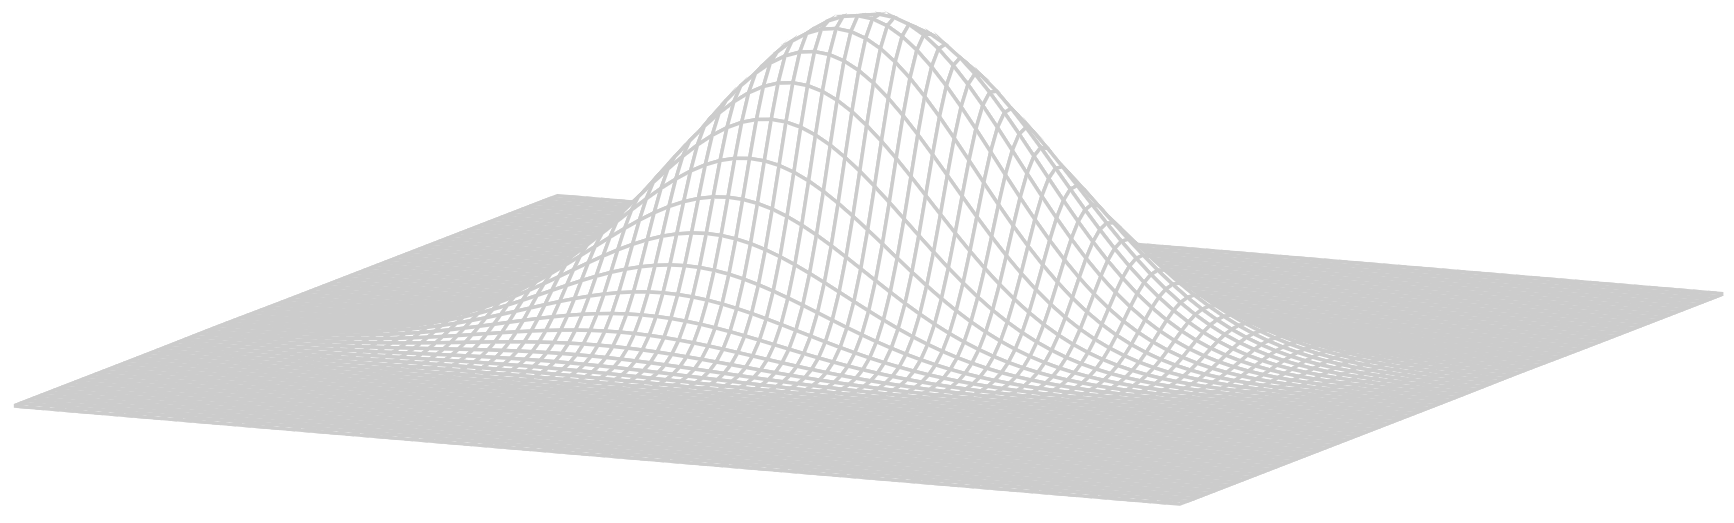
\includegraphics[scale=0.45]{bivar}
}\hfil}
Лінії рівня цієї поверхні задають \emph{еліпси розсіювання}:
$$f_{\vec{\xi}}(x,y) = C \Leftrightarrow \frac{(x-a_1)^2}{\sigma_1^2} -
2\rho\frac{x-a_1}{\sigma_1}\frac{y-a_2}{\sigma_2} +
\frac{(y-a_2)^2}{\sigma_2^2} = \lambda^2$$

\begin{tabular}{c p{7.8cm}}
\begin{tikzpicture}[baseline={(current bounding box.north)}]
    \draw [->] (-0.5, 0) -- (5, 0);
    \draw [->] (0, -0.5) -- (0, 3);
    \draw (2, 1.5) circle [x radius=1, y radius=0.5, rotate=40];
    \draw (2, 1.5) circle [x radius=1.3, y radius=0.7, rotate=40];
    \draw (2, 1.5) circle [x radius=1.5, y radius=0.9, rotate=40];
    \draw [fill] (2, 1.5) circle [radius = 0.05];
    \draw [<-] (3.5, 2.824) -- (0.3, 0);
    \draw [<-] (1, 2.64) -- (3, 0.38);
    \draw [dashed] (2, 1.5) -- (0, 1.5);
    \draw [dashed] (2, 1.5) -- (2, 0);
    \node [below] at (5, 0) {$x$};
    \node [left] at (0, 2.8) {$y$};
    \node [below] at (2, 0) {$a_1$};
    \node [left] at (0, 1.5) {$a_2$};
    \draw (0.6, 0) arc (0:40:0.3);
    \node [above right] at (0.55, 0) {$\alpha$};
\end{tikzpicture}&
$\mathrm{tg}2\alpha = \frac{2\rho\sigma_1\sigma_2}{\sigma_1^2 - \sigma_2^2}$\newline
Осі еліпсів називаються \emph{головними осями розсіювання}.\newline
Якщо $\rho = 0$, то головні осі розсіювання паралельні осям координат.
\end{tabular}

Позначимо $E_\lambda = \left\{(x;y) \in \mathbb{R}^2: \frac{(x-a_1)^2}{\sigma_1^2} -
2\rho\frac{x-a_1}{\sigma_1}\frac{y-a_2}{\sigma_2} +
\frac{(y-a_2)^2}{\sigma_2^2} \leq \lambda^2\right\}$.
Знайдемо ймовірність потрапляння в цю область у випадку $\rho = 0$:

\begin{gather*}
    P\left\{\vec{\xi} \in E_\lambda\right\} = \iint\limits_{E_\lambda} f_{\vec{\xi}}(x,y) dx dy = 
    \frac{1}{2\pi\sigma_1\sigma_2} \iint\limits_{E_\lambda} \exp\left\{-\frac{1}{2}\left( 
        \frac{(x-a_1)^2}{\sigma_1^2} + 
        \frac{(y-a_2)^2}{\sigma_2^2}
    \right)\right\} dx dy = \\
    \left[ \begin{gathered}
        x-a_1 = \lambda\sigma_1 r \cos\varphi \\ 
        y-a_2 = \lambda\sigma_2 r \sin\varphi \\
        |\mathcal{J}| = \lambda^2 \sigma_1 \sigma_2 r
    \end{gathered}\right] = 
    \frac{\lambda^2}{2\pi} \int\limits_0^{2\pi}  d\varphi
    \int\limits_0^1 r e^{-\frac{\lambda^2r^2}{2}} dr = 
    \int\limits_0^1 e^{-\frac{\lambda^2r^2}{2}} d\left(\frac{\lambda^2r^2}{2} \right) = 
    1 - e^{-\frac{\lambda^2}{2}}
\end{gather*}

\begin{exercise}
    Довести, що у випадку $\rho > 0$ $P\left\{\vec{\xi} \in E_\lambda\right\} = 
    1 - e^{-\frac{\lambda^2}{2(1-\rho^2)}}$.
\end{exercise}

\begin{example}
    $\vec{\xi} \sim \mathrm{N}\left( \begin{pmatrix}
        -1 \\ 1
    \end{pmatrix}, \begin{pmatrix}
        1 & 2 \\
        2 & 16
    \end{pmatrix}\right)$. Знайти рівняння еліпса розсіювання, для якого \\
    $P\left\{\vec{\xi} \in E_\lambda\right\} = 0.93$. З кореляційної матриці $\rho = 0.5$.
    Розв'яжемо відносно $\lambda^2$ рівняння $1 - e^{-\frac{\lambda^2}{2(1-0.5^2)}} = 0.93
    \Leftrightarrow e^{-\frac{\lambda^2}{1.5}} = 0.07 \Rightarrow \lambda^2 \approx 4$. Тому рівняння еліпса
    $\frac{(x+1)^2}{1} - \frac{x+1}{1} \frac{y-1}{4} + \frac{(y-1)^2}{16} = 4$ або 
    $\frac{(x+1)^2}{4} - \frac{(x+1)(y-1)}{16} + \frac{(y-1)^2}{64} = 1$.
\end{example}

Розглянемо гауссівський вектор $\vec{\xi} = (\xi_1, \xi_2)$ з незалежними координатами.
Для нього $F_{\vec{\xi}}(x,y) = F_{\xi_1}(x) F_{\xi_2}(y) = 
\left(\frac{1}{2} + \Phi\left( \frac{x-a_1}{\sigma_1}\right) \right)
\left(\frac{1}{2} + \Phi\left( \frac{y-a_2}{\sigma_2}\right) \right)$.
Тоді ймовірність потрапляння в прямокутник $\Pi = \left\{(x;y)\in\mathbb{R}^2 : \alpha \leq x < \beta, \gamma \leq y < \delta\right\}$
дорівнює $$\left( \Phi\left( \frac{\beta-a_1}{\sigma_1}\right) - \Phi\left( \frac{\alpha-a_1}{\sigma_1}\right)\right) \cdot
\left( \Phi\left( \frac{\delta-a_2}{\sigma_2}\right) - \Phi\left( \frac{\gamma-a_2}{\sigma_2}\right)\right)$$
\begin{exercise}
    Довести формулу для $P\left\{\vec{\xi}\in\Pi\right\}$.
\end{exercise}
Для гауссівського вектору з незалежними координатами також має місце <<правило $3\sigma$>>:
\begin{gather*}
    P\left\{\vec{\xi} \in (a_1-3\sigma_1; a_1+3\sigma_1)\times(a_2-3\sigma_2; a_2+3\sigma_2)\right\} = \\
    = P\left\{\xi_1 \in(a_1-3\sigma_1; a_1+3\sigma_1)\right\}\cdot P\left\{\xi_2 \in(a_2-3\sigma_2; a_2+3\sigma_2)\right\}
    \approx 0.9973^2 \approx 0.9946
\end{gather*}

\subsection{Колове розсіювання}
\begin{definition}
    Двовимірний гауссівський вектор має \emph{колове розсіювання}, якщо
    $\vec{a} = \vec{0}, \; K = \begin{pmatrix}
        \sigma^2 & 0 \\
        0 & \sigma^2
    \end{pmatrix}$. В цьому випадку $f_{\vec{\xi}} = \frac{1}{2\pi\sigma^2} \exp\left\{-\frac{x^2+y^2}{2\sigma^2}\right\}$, 
    а еліпси розсіювання стають колами.
\end{definition}
Знайдемо ймовірність потрапляння такого $\vec{\xi}$ в коло $K_R = \left\{(x; y) \in \mathbb{R}^2 : x^2 + y^2 \leq R^2\right\}$:
\begin{gather*}
    P\left\{\vec{\xi} \in K_R\right\} = \frac{1}{2\pi\sigma^2} \iint\limits_{K_R} e^{-\frac{x^2+y^2}{2\sigma^2}} dx dy = 
    \left[ \begin{gathered}
        x = \sigma r\cos\varphi \\
        y = \sigma r\sin\varphi \\
        |\mathcal{J}| = \sigma^2 r
    \end{gathered}\right] =
    \frac{1}{2\pi} \int\limits_0^{2\pi} d\varphi \int\limits_0^{R/\sigma} r e^{-\frac{r^2}{2}} dr = \\
    = \int\limits_0^{R/\sigma} e^{-\frac{r^2}{2}} d \left( \frac{r^2}{2}\right) = 
    1 - e^{-\frac{R^2}{2\sigma^2}}
\end{gather*}
Таким чином, тепер відомий розподіл норми $\vec{\xi}$. $\eta = \Vert \vec{\xi} \Vert = \sqrt{\xi_1^2 + \xi_2^2}$ --- випадкова величина,
для якої $F_{\eta}(R) = P\left\{\Vert \vec{\xi} \Vert < R\right\} = \begin{cases}
    1 - e^{-\frac{R^2}{2\sigma^2}}, & R > 0 \\
    0, & R \leq 0
\end{cases}$ --- це \emph{розподіл Релея}. Ця властивість переноситься й на довільну скінченну розмірність.

\begin{exercise}
    Знайти основні числові характеристики розподілу Релея.
\end{exercise}

\subsection{Умовний гауссівський розподіл на площині}
Знайдемо одну з умовних щільностей розподілу:
\begin{gather*}
    f_{\xi_1}(x/\xi_2 = y) = \frac{f_{\vec{\xi}}(x,y)}{f_{\xi_2}(y)} = 
    \frac{\frac{1}{2\pi\sigma_1\sigma_2\sqrt{1-\rho^2}} \exp\left\{
        -\frac{1}{2(1-\rho^2)}\cdot
        \left(\frac{(x-a_1)^2}{\sigma_1^2} -
        2\rho\frac{x-a_1}{\sigma_1}\frac{y-a_2}{\sigma_2} +
        \frac{(y-a_2)^2}{\sigma_2^2}
        \right)\right\} }{
            \frac{1}{\sqrt{2\pi}\sigma_2} \exp\left\{-\frac{1}{2\sigma_2^2}(y-a_2)^2\right\}
        } = \\
        \frac{1}{\sqrt{2\pi}\sigma_1\sqrt{1-\rho^2}} \exp\left\{
            -\frac{1}{2(1-\rho^2)}
        \left(\frac{(x-a_1)^2}{\sigma_1^2} -
        2\rho\frac{(x-a_1)(y-a_2)}{\sigma_1\sigma_2} +
        \frac{(y-a_2)^2}{\sigma_2^2}
        \right) +
        \frac{(y-a_2)^2}{2\sigma_2^2}
        \right\} = \\
        = \left [ \frac{(y-a_2)^2}{\sigma_2^2} - \frac{(1-\rho^2)(y-a_2)^2}{\sigma_2^2} = \rho^2 \frac{(y-a_2)^2}{\sigma_2^2}\right]=\\
        = \frac{1}{\sqrt{2\pi}\sigma_1\sqrt{1-\rho^2}} \exp\left\{-\frac{1}{2(1-\rho^2)}\left( \frac{x-a_1}{\sigma_1} - \rho\cdot\frac{y-a_2}{\sigma_2}\right)^2\right\} = \\
        = \frac{1}{\sqrt{2\pi}\sigma_1\sqrt{1-\rho^2}} \exp\left\{-\frac{1}{2\sigma_1^2(1-\rho^2)}\left( x- \left( a_1 + \frac{\rho\sigma_1(y-a_2)}{\sigma_2}\right)\right)^2\right\}
\end{gather*}
Аналогічно $f_{\xi_2}(y/\xi_1 = x) = \frac{1}{\sqrt{2\pi}\sigma_2\sqrt{1-\rho^2}} \exp\left\{-\frac{1}{2\sigma_2^2(1-\rho^2)}\left( y- \left( a_2 + \frac{\rho\sigma_2(x-a_1)}{\sigma_1}\right)\right)^2\right\}$.

\noindentОтже, обидві умовні щільності є щільностями нормального розподілу.

$E\left( \xi_1 / \xi_2 = y\right) = a_1 + \frac{\rho\sigma_1(y-a_2)}{\sigma_2}$, 
$E\left( \xi_2 / \xi_1 = x\right) = a_2 + \frac{\rho\sigma_2(x-a_1)}{\sigma_1}$. Лінії регресії --- прямі,

\noindent
$\rho\frac{\sigma_1}{\sigma_2} = \frac{K\xi_1\xi_2}{D\xi_2}$ та $\rho\frac{\sigma_2}{\sigma_1}  = \frac{K\xi_1\xi_2}{D\xi_1}$ --- відповідні кутові коефіцієнти прямих регресії.

$D\left( \xi_1 / \xi_2 = y\right) = \sigma_1^2(1-\rho^2)$, 
$D\left( \xi_2 / \xi_1 = x\right) = \sigma_2^2(1-\rho^2)$. Умовні дисперсії є сталими, ця властивість називається \emph{гомоскедастичністю}.
    % \chapter{Функції випадкових аргументів}
        % % !TEX root = ../main.tex

\section{Функції одного випадкового аргументу}
При розв'язанні задач іноді виникає необхідність визначити закон розподілу невипадкової функції від випадкового аргумента,
розподіл якого є відомим.
\subsection{Функції від дискретного випадкового аргументу}
Нехай $\xi$ --- дискретна випадкова величина з рядом розподілу 
\begin{center}
    \begin{tabular}{|c|c|c|c|c|c|}
        \hline
        $\xi$ & $x_1$ & $x_2$ & $...$ & $x_n$ & $...$ \\
        \hline
        $p$ & $p_1$ & $p_2$ & $...$ & $p_n$ & $...$ \\
        \hline
    \end{tabular}    
\end{center}
а $\varphi$ --- деяка вимірна числова функція, 
область визначення якої містить можливі значення $\xi$.
Можна розглядати випадкову величину $\eta = \varphi(\xi)$.

Очевидно, що $\eta$ --- теж ДВВ, що приймає значення $y_k = \varphi(x_k)$, 
$k = 1, 2, ...$ з ймовірностями $\P\{\eta = y_k\} = \P\{\xi = x_k : \varphi(x_k) = y_k\}$.
Якщо існує лише одне $\varphi^{-1} (y_k) = x_k$, то $\P\{\eta = y_k\} = \P\{\xi = x_k\} = p_k$.
Однак, можливо, що $y_k = \varphi(x_{k_1}) = \varphi(x_{k_2}) = ... = \varphi(x_{k_m})$.
Тоді $\P\{\eta = y_k\} = p_{k_1} + p_{k_2} + ... + p_{k_m}$.

\begin{example}
    Нехай $\xi$ має ряд розподілу
    \begin{center}
        \begin{tabular}{|c|c|c|c|c|c|}
            \hline
            $\xi$ & $-2$ & $-1$ & $0$ & $1$ & $2$ \\
            \hline
            $p$ & $1/9$ & $2/9$ & $1/9$ & $2/9$ & $3/9$ \\
            \hline
        \end{tabular}
    \end{center}
    Знайти закон розподілу $\eta = \xi^2$.
    
    З ряду розподілу $\xi$ видно, що $\xi^2$ приймає значення $0, 1, 4$ з
    ймовірностями $1/9$, $2/9 + 2/9$ та $1/9 + 3/9$.
    Отже, маємо ряд розподілу $\eta$: 
    \begin{center}
        \begin{tabular}{|c|c|c|c|}
            \hline
            $\eta$ & $0$ & $1$ & $4$ \\
            \hline
            $p$ & $1/9$ & $4/9$ & $4/9$ \\
            \hline
        \end{tabular}
    \end{center}
\end{example}

З побудови ряду розподілу функції від дискретного
випадкового аргументу випливає, що $\E(\varphi(\xi))^k = \sum\limits_{i=1}^{n(\infty)} \varphi^k(x_i) \P\{\xi = x_i\}$.

\subsection{Функції від неперервного випадкового аргументу}
Нехай $\xi$ --- неперервна випадкова величина, $f_\xi(x)$ --- її щільність розподілу, а $\varphi$ --- монотонна неперервна числова функція,
для якої обернена функція $\varphi^{-1}$ є диференційовною майже скрізь.
Розглянемо два випадки.

\begin{enumerate}
    \item $\eta = \varphi(\xi)$, де $\varphi$ --- монотонно зростаюча.

    \begin{tabular}{c p{8.8cm}}
        \begin{tikzpicture}[xscale = 0.7, yscale = 0.3, baseline={(current bounding box.north)}]
            \draw [->] (-3, 0) -- (3, 0);
            \draw [->] (0, -0.5) -- (0, 5.5);
            \draw [domain=-3:3, smooth, variable = \x, ultra thick] plot ({\x}, {e^(\x/2});
            \node [below] at (3, 0) {$x$};
            \node [left] at (0, 5.5) {$y$};
        \end{tikzpicture} &
        $F_\eta (y) = \P\left\{ \eta < y\right\} = \P\left\{ \varphi(\xi) < y\right\}$.

        Нехай $y = \varphi(x)$, тоді з монотонності $\varphi$ маємо рівність подій $\left\{ \varphi(\xi) < y\right\} = \left\{ \xi < x\right\}$.
        Тому $F_\eta (y) = F_\xi (x) = \int\limits_{-\infty}^x f_\xi(t) dt$. $\varphi$ має обернену, $x = \varphi^{-1} (y)$.
    \end{tabular}

    Отже, $F_\eta (y) = \int\limits_{-\infty}^{\varphi^{-1} (y)} f_\xi(t) dt$,
    $f_\eta(y) = F^\prime_\eta (y) = f_\xi\left(\varphi^{-1} (y)\right) \cdot \left(\varphi^{-1} (y) \right)^{\prime}$.
    \item $\eta = \varphi(\xi)$, де $\varphi$ --- монотонно спадна.
    
    \begin{tabular}{c p{8.8cm}}
        \begin{tikzpicture}[xscale = 0.7, yscale = 0.3, baseline={(current bounding box.north)}]
            \draw [->] (-3, 0) -- (3, 0);
            \draw [->] (0, -0.5) -- (0, 5.5);
            \draw [domain=-3:3, smooth, variable = \x, ultra thick] plot ({\x}, {e^(-\x/2});
            \node [below] at (3, 0) {$x$};
            \node [left] at (0, 5.5) {$y$};
        \end{tikzpicture} &
        $F_\eta (y) = \P\left\{ \eta < y\right\} = \P\left\{ \varphi(\xi) < y\right\}$.

        Нехай $y = \varphi(x)$, тоді з монотонності $\varphi$ маємо рівність подій $\left\{ \varphi(\xi) < y\right\} = \left\{ \xi > x\right\}$.
        Тому $F_\eta (y) = 1 - F_\xi (x) = 1 - \int\limits_{-\infty}^x f_\xi(t) dt$. $\varphi$ має обернену, $x = \varphi^{-1} (y)$.
    \end{tabular}

    Отже, $F_\eta (y) = 1 - \int\limits_{-\infty}^{\varphi^{-1} (y)} f_\xi(t) dt$,
    $f_\eta(y) = F^\prime_\eta (y) = - f_\xi\left(\varphi^{-1} (y)\right) \cdot \left(\varphi^{-1} (y) \right)^{\prime}$.
\end{enumerate}

\noindent Остаточно, для монотонної неперервної $\varphi$,
для якої обернена функція $\varphi^{-1}$ є диференційовною майже скрізь, має місце формула:
\begin{equation}\label{eq:phi_xi}
    \eta = \varphi(\xi), f_\eta(y) = f_\xi\left(\varphi^{-1} (y)\right) \cdot \left|\left(\varphi^{-1} (y) \right)^{\prime}\right|
\end{equation}
При цьому обов'язково треба зазначити допустимі значення $y$.

\begin{example}
    Нехай $\xi \sim \mathrm{U}(-\frac{\pi}{2}; \frac{\pi}{2})$. Знайти розподіл $\eta = \sin \xi$.

    \noindent $f_\xi(x) = \begin{cases}
        \frac{1}{\pi}, & |x| < \frac{\pi}{2} \\
        0, & |x| \geq \frac{\pi}{2}
    \end{cases}$, $\varphi(x) = \sin x$, $\varphi^{-1} (y) = \arcsin(y)$, $\left(\varphi^{-1} (y)\right)^{\prime} = \frac{1}{\sqrt{1-y^2}}$.
    $\eta$ може приймати значення від $-1$ до $1$. 
    Отже, $f_\eta(y) = \begin{cases}
        \frac{1}{\pi\sqrt{1-y^2}}, & |y| < 1 \\
        0, & |y| \geq 1
    \end{cases}$ --- це <<закон арксинуса>>.
\end{example}

\begin{example}
    Нехай $\xi \sim \mathrm{N}(a, \sigma^2)$. Знайти розподіл $\eta = e^\xi$.

    В цьому випадку $\varphi(x) = e^x$, $\varphi^{-1}(y) = \ln y$, $\left(\varphi^{-1} (y)\right)^{\prime} = \frac{1}{y}$.
    $\eta$ може приймати лише додатні значення, тому отримуємо щільність
    \begin{gather*}
        f_\eta(y) = \begin{cases}
            \frac{1}{\sqrt{2\pi}\sigma y} e^{-\frac{(\ln y-a)^2}{2\sigma^2}}, & y > 0 \\
            0, & y \leq 0
        \end{cases}
    \end{gather*}
    Розподіл $\eta$ називається \emph{логнормальним} (оскільки $\ln \eta$ має нормальний розподіл)
    та позначається $\eta \sim \mathrm{LogN}(a, \sigma^2)$.
\end{example}
\begin{exercise}
    Перевірити, що $\E\eta = e^{a + \frac{\sigma^2}{2}}$ і
    $\D\eta = \left(e^{\sigma^2} - 1\right) e^{2a + \sigma^2}$.
\end{exercise}

\begin{example}
    Нехай $\xi$ --- довільна НВВ, $F_\xi (x)$ --- її функція розподілу. 
    Знайти закон розподілу $\eta = F_\xi (\xi)$.

    \noindent $F_\eta (y) = \P\{\eta < y\} = \P\{F_\xi(\xi) < y\} = \P\{\xi < F_\xi^{-1}(y)\} = F_\xi(F_\xi^{-1}(y)) = \begin{cases}
        0, & y \leq 0 \\
        y, & 0 < y \leq 1 \\
        1, & y > 1
    \end{cases}$.

    \noindent Отже, $F_\xi (\xi) \sim U\left<0;1\right>$. Ще раз зауважимо, що результат має місце для довільної НВВ $\xi$.
\end{example}

\begin{remark}
    Якщо $\varphi$ не є неперервною, то $\eta = \varphi(\xi)$ може не бути НВВ. Наведемо декілька прикладів.
    \begin{enumerate}
        \item Нехай $\xi \sim \mathrm{Exp}(1)$. Знайдемо розподіл $\eta = \left[ \xi\right]$, де $\left[ \cdot\right]$ --- ціла частина.
        Оскільки ціла частина приймає значення $0, 1, 2, ...$, знайдемо відповідні ймовірності. 
        
        $\P\left\{ \left[ \xi\right] = n\right\} = \P\left\{ \xi \in [n; n+1)\right\} = \int\limits_n^{n+1} e^{-x} dx = e^{-n} - e^{-(n+1)} = e^{-n}(1 - e^{-1})$, $n = 0, 1, 2, ...$

        Отже, $\eta = \left[ \xi\right] \sim \mathrm{Geom}(1-e^{-1})$.

        За цим прикладом можна зробити висновок: якщо $\varphi$ --- кусково стала, а $\xi$ --- НВВ, то $\varphi(\xi)$ --- ДВВ.
        \item Нехай $\xi \sim \mathrm{Exp}(1)$. Знайдемо розподіл $\eta = \left\{ \xi\right\} = \xi - \left[ \xi\right]$. 
        В цьому випадку $\varphi$ є кусково неперервною функцією та приймає значення з інтервалу $[0; 1)$.
        
        Для $0< y < 1$ $F_\eta (y) = \P\left\{\eta < y\right\} = \P\left\{\eta \in [0; y)\right\} = \P\left\{\xi \in [n; n+y), n = 0, 1, 2, ...\right\}$.

        Для кожного $n$ $\P\left\{\xi \in [n; n+y)\right\} = \int\limits_n^{n+y} e^{-x} dx = e^{-n}(1 - e^{-y})$. 
        Отже, $\P\left\{\eta \in [0; y)\right\} = \sum\limits_{n=0}^{\infty} \P\left\{\xi \in [n; n+y)\right\} = (1 - e^{-y}) \sum\limits_{n=0}^{\infty} e^{-n} = \frac{1 - e^{-y}}{1 - e^{-1}}$. Отримали функцію розподілу $\eta$:

        $F_\eta (y) = \begin{cases}
            0, & y \leq 0 \\
            \frac{1 - e^{-y}}{1 - e^{-1}}, & 0 < y \leq 1 \\
            1, & y > 1
        \end{cases}$. Таким чином, $\eta$ --- НВВ.
    \end{enumerate}
\end{remark}

Узагальнимо формулу \eqref{eq:phi_xi} на випадок немонотонної функції $\varphi$.
Нехай $\xi$ --- НВВ, $f_\xi(x)$ --- її щільність розподілу, а $\varphi$ --- неперервна немонотонна числова функція.
Тоді область можливих значень $\xi$ можна розбити на проміжки, на яких $\varphi$ буде монотонною. 
Тоді, скориставшись результатом для монотонної функції, отримаємо формулу для щільності $\eta = \varphi(\xi)$:
\begin{equation}
    f_\eta (y) = \sum\limits_{k=1}^m f_\xi\left(\varphi_k^{-1} (y)\right) \cdot \left|\left(\varphi_k^{-1} (y) \right)^{\prime}\right|
\end{equation}
де $m$ --- кількість проміжків монотонності, а $\varphi_k^{-1}$ --- відповідні обернені функції, які мають бути диференційовними майже скрізь.

\begin{example}
    \begin{enumerate}
        \item $\xi \sim \mathrm{U}(-\frac{\pi}{2}, \frac{\pi}{2})$, знайти розподіл $\eta = \cos\xi$.

        На проміжках $(-\frac{\pi}{2}; 0]$ та $[0; \frac{\pi}{2})$ $\cos x$ є монотонною функцією, 
        відповідні обернені --- $\varphi_1^{-1} (y) = -\arccos y$, $\varphi_2^{-1} (y) = \arccos y$.

        Тоді $f_\eta (y) = \frac{1}{\pi} \cdot \left| - \frac{1}{\sqrt{1-y^2}}\right| + \frac{1}{\pi} \cdot \left|\frac{1}{\sqrt{1-y^2}}\right| = \begin{cases}
            \frac{2}{\pi} \frac{1}{\sqrt{1-y^2}}, & y \in [0; 1) \\
            0, & y \notin [0; 1)
        \end{cases}$.
        \item\label{ex:squared_norm_distr} $\xi \sim \mathrm{N}(a, \sigma)$, знайти розподіл $\eta = \xi^2$.

        На проміжках $(-\infty; 0]$ та $[0; +\infty)$ $x^2$ є монотонною функцією, 
        відповідні обернені --- $\varphi_1^{-1} (y) = -\sqrt{y}$, $\varphi_2^{-1} (y) = \sqrt{y}$.
        Щільність розподілу $\xi$ --- $f_\xi (x) = \frac{1}{\sqrt{2\pi}\sigma} e^{-\frac{(x-a)^2}{2\sigma^2}}$.

        Тоді $f_\eta (y) = \begin{cases}
            \frac{1}{\sqrt{2\pi}\sigma} e^{-\frac{(-\sqrt{y}-a)^2}{2\sigma^2}} \cdot \frac{1}{2\sqrt{y}} + 
        \frac{1}{\sqrt{2\pi}\sigma} e^{-\frac{(\sqrt{y}-a)^2}{2\sigma^2}} \cdot \frac{1}{2\sqrt{y}}, & y > 0 \\
        0, & y \leq 0
        \end{cases}$.

        При $\xi \sim \mathrm{N}(0, 1)$ $f_\eta(y) = \begin{cases}
            \frac{1}{\sqrt{2\pi y}} e^{-y/2}, y > 0 \\
            0, y \leq 0
        \end{cases}$, що означає $\xi^2 \sim \Gamma(\frac{1}{2}, \frac{1}{2})$.
    \end{enumerate}
\end{example}

\subsection{Числові характеристики функції неперервного випадкового аргументу}
Для функцій від ДВВ вже було отримано, що
$\E(\varphi(\xi))^k = \sum\limits_{i=1}^{n(\infty)} \varphi^k(x_i) \P\{\xi = x_i\}$.
Доведемо аналогічне твердження для функцій від НВВ.

\begin{proposition*}
    $\E (\varphi(\xi))^k = \int\limits_{-\infty}^{+\infty} \varphi^k(x) f_\xi(x) dx$ для всіх $k \in \mathbb{N}$.
\end{proposition*}
\begin{proof}
    Достатньо довести для монотонно зростаючої $\varphi$.

    \noindent$\eta = \varphi(\xi)$, $\E\eta^k = \int\limits_{-\infty}^{+\infty} y^k f_\eta(y) dy = \int\limits_{-\infty}^{+\infty} y^k f_\xi (\varphi^{-1} (y)) (\varphi^{-1} (y))^\prime dy =
    \int\limits_{-\infty}^{+\infty} y^k f_\xi(\varphi^{-1} (y)) d \varphi^{-1} (y) = \left[ \varphi^{-1} (y) = x, y = \varphi(x)\right] = \int\limits_{-\infty}^{+\infty} \varphi^k(x) f_\xi(x) dx$.
    У випадку монотонно спадної $\varphi$ під інтегралом отримаємо $-(\varphi^{-1} (y))^\prime$, а інтеграл після заміни змінної буде від $+\infty$ до $-\infty$.
    У випадку немонотонної $\varphi$ треба буде скористатися адитивністю інтеграла.
\end{proof}

\begin{remark}
    Для знаходження числових характеристик функції неперервного випадкового аргументу розподіл самої функції знаходити не потрібно.
\end{remark}

\begin{exercise}
    Дослідити, за яких умов на $\varphi$ ця формула має місце.
\end{exercise}

У випадках, коли $\varphi(x) = \cos (s x)$ або $\sin (s x)$ ($s\in \mathbb{R}$),
для знаходження числових характеристик можна скористатися характеристичною функцією $\xi$,
оскільки $\chi_{\xi}(s) = \E e^{i s \xi} = \E \cos(s\xi) + i \cdot\E\sin(s\xi)$,
тому $\E\cos(s\xi) = \mathrm{Re} \chi_{\xi}(s)$ і
$\E\sin(s\xi) = \mathrm{Im} \chi_{\xi}(s)$.
Для знаходження моментів вищих порядків можна скористатися формулами пониження степеня.
        % % !TEX root = ../main.tex

\section{Функції кількох випадкових аргументів}
\subsection{Випадок довільної функції}
Нехай $\varphi : \mathbb{R}^n \to \mathbb{R}$ --- задана вимірна числова функція.

Якщо $\vec{\xi} = \left(\xi_1, ..., \xi_n\right)^T$ --- дискретний випадковий вектор, тоді $\eta = \varphi(\vec{\xi})$ --- ДВВ.
Побудову закону розподілу $\eta$ доцільно розглянути на прикладі.
\begin{example}
    $\vec{\xi} = \left( \xi_1, \xi_2\right)$ задано таблицею розподілу:
    \begin{center}
        \begin{tabular}{|c|c|c|c|}
            \hline
            \diagbox{$\xi_2$}{$\xi_1$} & $0$ & $1$ & $2$ \\
            \hline
            $-1$ & $0.1$ & $0.2$ & $0.3$ \\
            \hline
            $1$ & $0.2$ & $0.1$ & $0.1$ \\
            \hline
        \end{tabular}    
    \end{center}

    \noindentЗнайдемо закони розподілу $\eta_1 = \xi_1 \xi_2$ та $\eta_2 = \xi_1 + \xi_2$.
    Для цього треба визначити значення, які приймають ці величини, та обчислити відповідні ймовірності.
    
    $\eta_1$ приймає значення $-2$ (коли $\xi_1 = 2$, $\xi_2 = -1$), 
    $-1$ (коли $\xi_1 = 1$, $\xi_2 = -1$), 
    $0$ (коли $\xi_1 = 0$, $\xi_2 = -1$ або $\xi_2 = 1$), 
    $1$ (коли $\xi_1 = 1$, $\xi_2 = 1$), 
    $2$ (коли $\xi_1 = 2$, $\xi_2 = 1$).

    $\eta_2$ приймає значення $-1$ (коли $\xi_1 = 0$, $\xi_2 = -1$), 
    $0$ (коли $\xi_1 = 1$, $\xi_2 = -1$), 
    $1$ (коли $\xi_1 = 0$, $\xi_2 = 1$ або $\xi_1 = 2$, $\xi_2 = -1$), 
    $2$ (коли $\xi_1 = 1$, $\xi_2 = 1$), 
    $3$ (коли $\xi_1 = 2$, $\xi_2 = 1$).
    Відповідні сумісні ймовірності отримуємо з таблиці розподілу $\vec{\xi}$. Отже,
    $\eta_1$ та $\eta_2$ мають наступні ряди розподілу:
    \begin{center}
        \begin{tabular}{|c|c|c|c|c|c|}
            \hline
            $\eta_1$ & $-2$ & $-1$ & $0$ & $1$ & $2$ \\
            \hline
            $p$ & $0.3$ & $0.2$ & $0.3$ & $0.1$ & $0.1$ \\
            \hline
        \end{tabular}
        \begin{tabular}{|c|c|c|c|c|c|}
            \hline
            $\eta_2$ & $-1$ & $0$ & $1$ & $2$ & $3$ \\
            \hline
            $p$ & $0.1$ & $0.2$ & $0.5$ & $0.1$ & $0.1$ \\
            \hline
        \end{tabular}
    \end{center}
\end{example}

Якщо $\vec{\xi} = \left(\xi_1, ..., \xi_n\right)^T$ --- неперервний випадковий вектор
із щільністю $f_{\vec{\xi}} (\vec{x})$, то можна знайти функцію розподілу $\eta = \varphi(\vec{\xi})$:
$$F_\eta (y) = \P \left\{ \eta < y\right\} = \P \left\{ \vec{\xi} \in D_y\right\} = \underset{D_y}{\int ... \int} f_{\vec{\xi}} (\vec{x}) d \vec{x}, \text{ де }D_y = \left\{\vec{x} \in \mathbb{R}^n : \varphi(\vec{x}) < y\right\}$$

Розглянемо тепер взаємно однозначне гладке перетворення $\vec{\psi} : \mathbb{R}^n \to \mathbb{R}^n$ та
знайдемо щільність розподілу $\vec{\eta} = \vec{\psi} (\vec{\xi})$. Для множини $D \subset \mathbb{R}^n$
$\P\left\{ \vec{\psi} (\vec{\xi}) \in D\right\} = \P\left\{ \vec{\xi} \in \vec{\psi}^{-1}(D)\right\} = \int_{\vec{\psi}^{-1}(D)} f_{\vec{\xi}} (\vec{x}) d\vec{x} = 
\left[ \text{заміна }\vec{y} = \vec{\psi}(\vec{x})\right] = \int_D f_{\vec{\xi}} (\vec{\psi}^{-1}(\vec{y})) \left| \mathcal{J}^{-1} (\vec{\psi}^{-1}(\vec{y})\right| d\vec{y}$,
де $\mathcal{J} (\vec{x})$ --- якобіан $\vec{\psi}$. Отже,
\begin{equation}
    f_{\vec{\eta}} (\vec{y}) = f_{\vec{\xi}} (\vec{\psi}^{-1}(\vec{y})) \left| \mathcal{J}^{-1} (\vec{\psi}^{-1}(\vec{y})\right|
\end{equation}
Як в одновимірному випадку, треба вказувати, які значення може приймати $\vec{\eta}$.

\begin{example}
    Нехай $A$ --- невироджена матриця розміру $n \times n$, $\vec{b} \in \mathbb{R}^n$ --- деякий вектор, $\vec{\xi}$ --- неперервний випадковий вектор.
    Знайти щільність розподілу $\vec{\eta} = A \vec{\xi} + \vec{b}$.

    В цьому випадку $\vec{y} = \vec{\psi}(\vec{x}) = A \vec{x} + \vec{b}$, тому $\vec{\psi}^{-1} (\vec{y}) = A^{-1} (\vec{y} - \vec{b})$. Якобіан $\vec{\psi}$ рівний $\left| \det A\right|$. 
    Отже,
    $f_{\vec{\eta}}(\vec{y}) = \frac{1}{\left| \det A\right|} f_{\vec{\xi}}\left(A^{-1} (\vec{y} - \vec{b})\right)$
\end{example}

Далі розглянемо конкретні приклади числових функцій від випадкових векторів.

\subsection{Закон розподілу мінімуму та максимуму}

Нехай випадкові величини $\xi_1, ..., \xi_n$ незалежні та однаково розподілені, як деяка випадкова величина $\xi$.
Знайдемо розподіл їх мінімуму та максимуму.
\begin{enumerate}
    \item Нехай $\mu_1 = \min\left\{\xi_1, \xi_2, ..., \xi_n\right\}$.
    \begin{gather*}
        F_{\mu_1} (x) = \P \left\{ \min\{\xi_1, \xi_2, ..., \xi_n\} < x \right\} =
        1 - \P \left\{ \min\{\xi_1, \xi_2, ..., \xi_n\} \geq x \right\} = \\ =
        1 - \P \left\{ \xi_1 \geq x, \xi_2 \geq x, ..., \xi_n \geq x \right\} = 
        1 - \P\left\{ \xi_1 \geq x\right\} \cdot \P\left\{ \xi_2 \geq x\right\} \cdot ... \cdot \P\left\{ \xi_n \geq x\right\} = \\
        = 1 - (\P\left\{ \xi \geq x\right\})^n = 1 - (1- F_\xi (x))^n
    \end{gather*}

    Якщо $\xi_1, ..., \xi_n$ --- неперервні, то $f_{\mu_1} (x) = \left( F_{\mu_1} (x)\right)^\prime = n (1- F_\xi (x))^{n-1} f_\xi(x)$.
    \item Нехай $\mu_2 = \max\left\{\xi_1, \xi_2, ..., \xi_n\right\}$.
    \begin{gather*}
        F_{\mu_2} (x) = \P \left\{ \max\{\xi_1, \xi_2, ..., \xi_n\} < x \right\} =
        \P \left\{ \xi_1 < x, \xi_2 < x, ..., \xi_n < x \right\} = \\ =
        \P\left\{ \xi_1 < x\right\} \cdot \P\left\{ \xi_2 < x\right\} \cdot ... \cdot \P\left\{ \xi_n < x\right\} =
        (\P\left\{ \xi < x\right\})^n = (F_\xi (x))^n
    \end{gather*}

    Якщо $\xi_1, ..., \xi_n$ --- неперервні, то $f_{\mu_2} (x) = \left( F_{\mu_2} (x)\right)^\prime = n (F_\xi (x))^{n-1} f_\xi(x)$.
\end{enumerate}

\begin{example}
    Нехай $\xi_1, ..., \xi_n$ незалежні та мають розподіл $\mathrm{Exp}(\lambda)$. Знайти розподіл їх мінімуму.
    За отриманими формулами запишемо щільність:

    $f_{\min}(x) = n (1-(1-e^{-\lambda x}))^{n-1} \lambda e^{-\lambda x} = n \lambda e^{-n\lambda x}$ при $x \geq 0$ та $0$ при $x < 0$.
    
    \noindentОтже, $\min\{\xi_1, ..., \xi_n\} \sim \mathrm{Exp} (n \lambda)$.
\end{example}

\subsection{Закон розподілу добутку двох НВВ}
Нехай $\vec{\xi} = (\xi_1, \xi_2)^T$ --- неперервний випадковий вектор, щільність
$f_{\vec{\xi}}(x, y)$ відома.

\noindent\textbf{Задача}: знайти розподіл $\eta = \xi_1\xi_2$.

Знайдемо функцію розподілу за вже відомою схемою:

$$F_\eta(z) = \iint\limits_{D_z}f_{\vec{\xi}}(x, y)dx dy, D_z = \left\{(x, y) \in 
\mathbb{R}^2 : xy < z\right\}$$

Розглянемо два варіанти:
\begin{enumerate}
    \item 
\begin{tabular}{c p{8.8cm}}
    \begin{tikzpicture}[baseline={(current bounding box.north)} ,scale = 0.4]
        \draw [domain=0.2:5, smooth, variable = \x, ultra thick] plot ({\x}, 
        {
            1/\x
        });
        \fill [lightgray, domain=0.2:5, smooth, variable = \x] plot ({\x}, 
        {
            1/\x
        }) -- (5, -5) -- (0, -5) -- (0, 5) -- (0.2, 5);
        \draw [domain=-5:-0.2, smooth, variable = \x, ultra thick] plot ({\x}, 
        {
            1/\x
        });
        \fill [lightgray, domain=-5:-0.2, smooth, variable = \x] plot ({\x}, 
        {
            1/\x
        }) -- (0, -5) -- (0, 5) -- (-5, 5) -- (-5, -0.2);
        \draw [->] (-5, 0) -- (5, 0);
        \draw [->] (0, -5) -- (0, 5);
        \node [below left] at (5, 0) {$x$};
        \node [below left] at (0, 5) {$y$};
        \node [above left] at (5, -5) {$D_z$};
        \node [above right] at (1, 1) {$y = \frac{z}{x}$};
    \end{tikzpicture} &
    $z > 0$, тоді $D_z = 
    \left\{x<0, y>\frac{z}{x}\right\} \cup 
    \left\{x>0, y<\frac{z}{x}\right\}$.

    $F_\eta (z) = \int\limits^{0}_{-\infty}dx\int\limits_{\frac{z}{x}}^{+\infty}
    f_{\vec{\xi}}(x, y) dy + \int\limits_0^{+\infty}dx\int\limits_{-\infty}^{\frac{z}{x}} 
    f_{\vec{\xi}}(x, y) dy$.

    Продиференціюємо обидві частини по $z$:

    $f_\eta(z) = -\int\limits_{-\infty}^0 \frac{1}{x}f_{\vec{\xi}}\left(x, \frac{z}{x}\right)dx + 
    \int\limits_0^{+\infty}\frac{1}{x}f_{\vec{\xi}}\left(x, \frac{z}{x}\right)dx$.
\end{tabular}

\item
\begin{tabular}{c p{8.8cm}}
    \begin{tikzpicture}[baseline={(current bounding box.north)} ,scale = 0.4]
        \draw [domain=0.2:5, smooth, variable = \x, ultra thick] plot ({\x}, 
        {
            -1/\x
        });
        \fill [lightgray, domain=0.2:5, smooth, variable = \x] plot ({\x}, 
        {
            -1/\x
        }) -- (5, -5) -- (0.2, -5);
        \draw [domain=-5:-0.2, smooth, variable = \x, ultra thick] plot ({\x}, 
        {
            -1/\x
        });
        \fill [lightgray, domain=-5:-0.2, smooth, variable = \x] plot ({\x}, 
        {
            -1/\x
        }) -- (-5, 5) -- (-5, 0.2);
        \draw [->] (-5, 0) -- (5, 0);
        \draw [->] (0, -5) -- (0, 5);
        \node [above left] at (5, 0) {$x$};
        \node [below right] at (0, 5) {$y$};
        \node [above left] at (5, -5) {$D_z$};
        \node [above right] at (1, 1) {$y = \frac{z}{x}$};
    \end{tikzpicture}
    &
    $z < 0$, тоді $D_z = 
    \left\{x<0, y>\frac{z}{x}\right\} \cup 
    \left\{x>0, y<\frac{z}{x}\right\}$.

    $F_\eta(z) = \int\limits_{-\infty}^0 dx \int\limits_{\frac{z}{x}}^{+\infty} 
    f_{\vec{\xi}}(x, y)dy + \int\limits_0^{+\infty}dx\int\limits_{-\infty}^{\frac{z}{x}} 
    f_{\vec{\xi}}(x, y) dy$
    
    Продиференціюємо обидві частини по $z$:

    $f_\eta(z) = - \int\limits_{-\infty}^0 \frac{1}{x} f_{\vec{\xi}}\left(x, \frac{z}{x}\right)dx 
    + \int\limits_0^{+\infty}\frac{1}{x}f_{\vec{\xi}}\left(x, \frac{z}{x}\right)dx$

\end{tabular}
\end{enumerate}

\vspace{0.5em}
\noindentОтже, отримали щільність добутку $\xi_1 \xi_2$:
\begin{equation}\label{eq:distr_product}
    f_{\xi_1 \xi_2}(z) = -\int\limits_{-\infty}^0 \frac{1}{x}f_{\vec{\xi}}\left(x, \frac{z}{x}\right)dx + 
    \int\limits_0^{+\infty}\frac{1}{x}f_{\vec{\xi}}\left(x, \frac{z}{x}\right)dx
\end{equation}

\begin{remark}
    Якщо $\xi_1$ та $\xi_2$ незалежні, то $f_{\vec{\xi}}\left(x, \frac{z}{x}\right) = 
    f_{\xi_1}(x)f_{\xi_2}\left(\frac{z}{x}\right)$.
\end{remark}

\begin{example}
    Нехай $\vec{\xi} = (\xi_1, \xi_2)^T$ рівномірно розподілений в квадраті $K = [0; 2]\times[0; 2]$.
    Знайти закон розподілу $\eta = \xi_1 \xi_2$.

    \begin{center}
        \begin{tabular}{c p{4.5cm}}
            \begin{tikzpicture}[baseline={(current bounding box.center)} ,scale = 1]
                \draw [black, ultra thick] 
                (0, 0) -- (2, 0) -- (2, 2) -- (0, 2) -- (0, 0);
                \fill [lightgray] 
                (0, 0) -- (2, 0) -- (2, 2) -- (0, 2) -- (0, 0);
                \draw [->] (-0.5, 0) -- (3, 0);
                \draw [->] (0, -0.5) -- (0, 3);
                \node [below left] at (3, 0) {$x$};
                \node [below left] at (0, 3) {$y$};
                \node [above right] at (0, 0) {$K$};
                \node [left] at (0, 2) {$2$};
                \node [below] at (2, 0) {$2$};
                \node [below left] at (0, 0) {$0$};
            \end{tikzpicture} 
            &
            $f_{\vec{\xi}}(x, y) = 
            \begin{cases}
                \frac{1}{4}, & (x, y) \in K \\
                0, & (x, y) \notin K
            \end{cases}
            $
        \end{tabular}
    \end{center}
    
    В цьому випадку простіше знайти функцію розподілу з геометричних міркувань, а не застосовувати формулу \eqref{eq:distr_product}:
    $F_{\eta}(z) = \P\{\xi_1\xi_2 < z\} = \iint\limits_{\{xy < z\}} f_{\vec{\xi}}(x, y)dxdy$. При $z<0$ $F_{\eta}(z) = 0$,
    а при $z \geq 4$ $F_{\eta}(z) = 1$.

        \begin{tabular}{c p{8.5 cm}}
            \begin{tikzpicture}[baseline={(current bounding box.north)}, scale = 0.9]
                \fill [lightgray, domain=0.5:2, smooth, variable = \x] plot ({\x}, 
                {
                    1/\x
                }) -- (2, 0) -- (0, 0) -- (0, 2) -- (0.5, 2);
                \draw [domain=0.333:3, smooth, variable = \x, thick] plot ({\x}, 
                {
                    1/\x
                });
                \draw [black, thick] 
                (0, 0) -- (2, 0) -- (2, 2) -- (0, 2) -- (0, 0);
                
                \draw [black, dashed] (0.5, 0) -- (0.5, 2);
                \draw [->] (-0.5, 0) -- (3, 0);
                \draw [->] (0, -0.5) -- (0, 3);
                \node [below left] at (3, 0) {$x$};
                \node [below left] at (0, 3) {$y$};
                \node [below] at (0.5, 0) {$\frac{z}{2}$};
                \node [left] at (0, 2) {$2$};
                \node [below] at (2, 0) {$2$};
                \node [below left] at (0, 0) {$0$};
                \node [above right] at (0.5, 2) {$y = \frac{z}{x}$};
                \node [above left] at (2, 0) {$D_z \cap K$};
            \end{tikzpicture} 
            &
            $F_{\eta}(z) = \frac{1}{4}S_{D_z \cap K} = \frac{1}{4} 
            \left(4 - \int\limits_{\frac{z}{2}}^2dx
            \int\limits_{\frac{z}{x}}^2dy\right) = $

            $=\frac{1}{4}\left(4 - \int\limits_{\frac{z}{2}}^2 
            \left(2 -\frac{z}{x}\right)dx\right) $

            \vspace{0.2em}
            $= 1 - \frac{1}{4}\left.(2x - z \ln x)\right|_{\frac{z}{2}}^2 = $
            
            \vspace{0.2em}
            $= 1 - \frac{1}{4}(4 - z\ln2 - z + z\ln\frac{z}{2}) =$
            
            \vspace{0.2em}
            $= \frac{1}{4}(z + z\ln2 - z\ln z + z\ln2) = $
            
            \vspace{0.2em}
            $= \frac{1}{4}(z + 2z\ln2 - z\ln z)$ 
            при $z\in [0; 4)$. \\
            Отже, $f_{\eta}(z) = 
            \begin{cases}
                0, & z \notin (0, 4] \\
                \frac{1}{4}(2\ln2 - \ln z), & z \in (0, 4]
            \end{cases}$.
        \end{tabular}
\end{example}

\subsection{Закон розподілу частки двох НВВ}

Нехай $\vec{\xi} = (\xi_1, \xi_2)^T$ --- неперервний випадковий вектор, щільність
$f_{\vec{\xi}}(x, y)$ відома.

\noindent\textbf{Задача}: знайти розподіл $\eta = \frac{\xi_2}{\xi_1}$.

Знайдемо функцію розподілу за вже відомою схемою:

$$F_\eta(z) = \iint\limits_{D_z}f_{\vec{\xi}}(x, y)dx dy, D_z = \left\{(x, y) \in 
\mathbb{R}^2 : \frac{y}{x} < z\right\}$$

\begin{enumerate}
    \item 
\begin{tabular}{c p{8.8cm}}
    \begin{tikzpicture}[baseline={(current bounding box.north)}, scale = 0.4]
        \fill [lightgray] (0, 5) -- (-5, 5) -- (-5, -5) -- (0, 0);
        \fill [lightgray] (5, -5) -- (0, -5) -- (0, 0) -- (5, 5);
        \draw [domain=-5:5, smooth, variable = \x, thick] plot ({\x}, 
        {
            \x
        });
        \draw [->] (-5, 0) -- (5, 0);
        \draw [->] (0, -5) -- (0, 5);
        \node [below left] at (5, 0) {$x$};
        \node [below left] at (0, 5) {$y$};
        \node [above left] at (5, -5) {$D_z$};
        \node [above left] at (3.7, 3) {$y = zx$};
    \end{tikzpicture} &
    $z > 0$, тоді $D_z = 
    \left\{x<0, y>z x\right\} \cup 
    \left\{x>0, y<z x\right\}$

    $F_\eta(z) = \int\limits_{-\infty}^0 dx \int\limits_{zx}^{+\infty}f_{\vec{\xi}}(x, y)dy 
    + \int\limits_0^{+\infty}dx\int\limits_{-\infty}^{zx}f_{\vec{\xi}}(x, y)dy$

    Продиференціюємо обидві частини по $z$:

    $f_\eta(z) = -\int\limits_{-\infty}^0 x f_{\vec{\xi}}(x, zx) dx + \int\limits_0^{+\infty}
    xf_{\vec{\xi}}(x, zx)dx$
\end{tabular}

\item 
\begin{tabular}{c p{8.8cm}}
    \begin{tikzpicture}[baseline={(current bounding box.north)} ,scale = 0.4]
        \fill [lightgray] (0, 0) -- (0, 5) -- (-5, 5);
        \fill [lightgray] (0, 0) -- (0, -5) -- (5, -5);
        \draw [domain=-5:5, smooth, variable = \x, thick] plot ({\x}, 
        {
            -\x
        });
        \draw [->] (-5, 0) -- (5, 0);
        \draw [->] (0, -5) -- (0, 5);
        \node [below left] at (5, 0) {$x$};
        \node [below left] at (0, 5) {$y$};
        \node [above left] at (4, -5) {$D_z$};
        \node [above right] at (2.6, -3) {$y = zx$};
    \end{tikzpicture} &
    $z < 0$, тоді $D_z = 
    \left\{x<0, y>z x\right\} \cup 
    \left\{x>0, y<z x\right\}$

    $F_\eta(z) = \int\limits_{-\infty}^0 dx \int\limits_{zx}^{+\infty}f_{\vec{\xi}}(x, y) dy +
    \int\limits_0^{+\infty}dx\int\limits_{-\infty}^{zx}f_{\vec{\xi}}(x, y)dy $

    Продиференціюємо обидві частини по $z$:

    $f_\eta(z) = -\int\limits_{-\infty}^0 x f_{\vec{\xi}}(x, zx)dx + \int\limits_0^{+\infty}
    xf_{\vec{\xi}}(x, zx)dx$
\end{tabular}
\end{enumerate}

\noindentОтже, отримали щільність частки $\frac{\xi_2}{\xi_1}$ 
\begin{equation}\label{eq:distr_frac}
    f_{\frac{\xi_2}{\xi_1}} (z)= -\int\limits_{-\infty}^0 xf_{\vec{\xi}}(x, zx)dx + 
    \int\limits_0^{+\infty}xf_{\vec{\xi}}(x, zx)dx    
\end{equation}

\begin{remark}
    Якщо $\xi_1$ та $\xi_2$ незалежні, то $f_{\vec{\xi}}(x, zx) = 
    f_{\xi_1}(x)f_{\xi_2}(zx)$.
\end{remark}

\begin{exercise}
    Перевірити, що щільність розподілу $\frac{\xi_1}{\xi_2}$ має вигляд
    \begin{equation}
        f_{\frac{\xi_1}{\xi_2}}(z) = -\int\limits_{-\infty}^0 y f_{\vec {\xi}}(zy, y) dy + \int\limits_0^{+\infty}
        yf_{\vec{\xi}}(zy, y)dy
    \end{equation}
\end{exercise}

\begin{example}
    Нехай $\xi_1$ та $\xi_2$ --- незалежні випадкові величини, що мають розподіл $\mathrm{N}(0, \sigma^2)$. Знайти закон розподілу $\eta = \frac{\xi_2}{\xi_1}$.

    \noindentСкористаємося знайденою формулою \eqref{eq:distr_frac}, враховуючи незалежність:
    \begin{gather*}
        f_\eta(z) = - \int\limits_{-\infty}^0 x f_{\xi_1}(x) f_{\xi_2}(zx) dx + 
        \int\limits_{0}^{+\infty} x f_{\xi_1}(x) f_{\xi_2}(zx) dx = 
        \\
        =
        -\frac{1}{2\pi\sigma^2}\int\limits_{-\infty}^0 x e^{-\frac{x^2}{2\sigma^2}\left(1+z^2\right)} dx
        +
        \frac{1}{2\pi\sigma^2}\int\limits_0^{+\infty} x e^{-\frac{x^2}{2\sigma^2}\left(1+z^2\right)}dx = 
        \\
        = \left[
        \begin{array}{c}
            \frac{x^2}{2\sigma^2}\left(1+z^2\right) = t \\
            \frac{x}{\sigma^2}\left(1+z^2\right)dx = dt 
        \end{array}
        \right]
        =
        \frac{-\sigma^2}{2\pi\sigma^2\left(1+z^2\right)}\int\limits_{+\infty}^0 e^{-t} dt
        +
        \frac{\sigma^2}{2\pi\sigma^2\left(1+z^2\right)}\int\limits^{+\infty}_0 e^{-t} dt = 
        \\
        = \frac{1}{\pi(1+z^2)}\int\limits_0^{+\infty}e^{-t}dt = \frac{1}{\pi(1+z^2)}, z \in \mathbb{R}
        \text{ --- це щільність розподілу Коші.} 
    \end{gather*}\index{розподіл!Коші}
\end{example}

\subsection{Закон розподілу суми двох НВВ}

Нехай $\vec{\xi} = (\xi_1, \xi_2)^T$ --- неперервний випадковий вектор, щільність
$f_{\vec{\xi}}(x, y)$ відома.

\noindent\textbf{Задача}: знайти розподіл $\eta = \xi_1 + \xi_2$.

Знайдемо функцію розподілу за вже відомою схемою:

$$F_\eta(z) = \iint\limits_{D_z}f_{\vec{\xi}}(x, y)dx dy, D_z = \left\{(x, y) \in 
\mathbb{R}^2 : x + y < z\right\}$$

\begin{tabular}{c p{8.8cm}}
    \begin{tikzpicture}[baseline={(current bounding box.north)} ,scale = 0.4]
        \fill [lightgray, domain=-5:5, smooth, variable = \x] 
        (-4, 5) -- (5, -4) -- (5, -5) -- (-5, -5) -- (-5, 5) -- (-4, 5);
        \draw [domain=-4:5, smooth, variable = \x, thick] plot ({\x}, 
        {
            1 - \x
        });
        \draw [->] (-5, 0) -- (5, 0);
        \draw [->] (0, -5) -- (0, 5);
        \node [below left] at (5, 0) {$x$};
        \node [below left] at (0, 5) {$y$};
        \node [above left] at (-1, 0) {$D_z$};
        \node [above right] at (0.5, 0) {$y = z - x$};
    \end{tikzpicture} &

    $F_\eta(z) = \int\limits_{-\infty}^{+\infty} dx \int\limits_{-\infty}^{z-x} 
    f_{\vec{\xi}}(x, y) dy$

    Продиференціюємо обидві частини по $z$:

    $f_\eta(z) = \int\limits_{-\infty}^{+\infty} f_{\vec{\xi}}(x, z-x) dx$
\end{tabular}

\vspace{0.5em}
\noindentОтже, отримали щільність суми $\xi_1 + \xi_2$:
\begin{equation}\label{eq:distr_sum}
    f_{\xi_1 + \xi_2}(z) = \int\limits_{-\infty}^{+\infty} f_{\vec{\xi}}(x, z-x) dx
\end{equation}

\begin{remark}
    Якщо $\xi_1$ та $\xi_2$ незалежні, то $f_{\xi_1 + \xi_2} (z) = 
    \int\limits_{-\infty}^{+\infty}f_{\xi_1}(x) f_{\xi_2}(z-x) dx = 
    (f_{\xi_1} \ast f_{\xi_2})(z)$. Тут $\ast$ позначає операцію 
    \href{https://uk.wikipedia.org/wiki/%D0%97%D0%B3%D0%BE%D1%80%D1%82%D0%BA%D0%B0_(%D0%BC%D0%B0%D1%82%D0%B5%D0%BC%D0%B0%D1%82%D0%B8%D1%87%D0%BD%D0%B8%D0%B9_%D0%B0%D0%BD%D0%B0%D0%BB%D1%96%D0%B7)}{згортки},
    що вводиться в курсі гармонічного аналізу.
\end{remark}

\begin{exercise}
    Перевірити, що щільність розподілу $\eta_1 = \xi_1 - \xi_2$ має вигляд
    $f_{\eta_1}(z) = \int\limits_{-\infty}^{+\infty} f_{\vec{\xi}}(x, x-z) dx$, а 
    $\eta_2 = \xi_2 - \xi_1$ --- $f_{\eta_2}(z) = \int\limits_{-\infty}^{+\infty} f_{\vec{\xi}}(x, x+z) dx$.
\end{exercise}

\begin{example}
    $\xi_1$ та $\xi_2$ --- незалежні випадкові величини, $\xi_i \sim \mathrm{Exp}(\lambda_i)$, 
    $i = 1,2$, $\lambda_1 \neq \lambda_2$.

    \noindentЗнайти закон розподілу $\eta = \xi_1 + \xi_2$.

    \noindentСкористаємося знайденою формулою \eqref{eq:distr_sum}, враховуючи незалежність:
    \begin{equation*}
        f_\eta(z) = \left[z - x > 0 \Rightarrow x < z\right] = 
        \int\limits_0^z \lambda_1 e^{-\lambda_1 x}\lambda_2e^{-\lambda_2(z-x)}dx
        =
        \lambda_1\lambda_2e^{-\lambda_2z}\int\limits_0^z e^{-x(\lambda_1 - \lambda_2)} dx=
    \end{equation*}
    \begin{equation*}
        =\lambda_1\lambda_2e^{-\lambda_2z}
        \left.
        \left(\frac{1}{-(\lambda_1 - \lambda_2)} e^{-x(\lambda_1 - \lambda_2)}\right)
        \right|_0^z = 
        \frac{\lambda_1\lambda_2}{\lambda_2 - \lambda_1}e^{-\lambda_2z}
        (e^{-z(\lambda_1 - \lambda_2)} - 1) =
    \end{equation*}
    \begin{equation*}
        = \frac{\lambda_1\lambda_2}{\lambda_2 - \lambda_1}(e^{-\lambda_1 z} - e^{-\lambda_2 z})
        ,\; z \geq 0 \text{ та } 0 \text{ інакше.}
    \end{equation*}
Це щільність так званого \emph{закону Ерланга 2-го порядку} \index{розподіл!Ерланга}.
\noindentПри $\lambda_1 = \lambda_2 = \lambda$ отримаємо
$f_{\eta}(z) = \lambda^2 z e^{-\lambda z}$ при $z \geq 0$ та $0$ інакше.
Це вже буде щільність гамма-розподілу $\Gamma(2, \lambda)$.
\end{example}

\subsection{Числові характеристики функції багатьох випадкових аргументів}
Розглядаємо неперервний випадковий вектор $\vec{\xi} = (\xi_1, \xi_2, ..., \xi_n)$ та
випадкову величину $\eta = \varphi(\vec{\xi})$.
\begin{exercise}
    Довести, що для НВВ $\eta$, що приймає невід'ємні значення, $\E\eta = \int\limits_0^{+\infty} (1 - F_{\eta}(x)) dx$.
\end{exercise}

\begin{proposition*} 
    $\E\eta^k = \int_{\mathbb{R}^n} \varphi^k(\vec{x}) f_{\vec{\xi}} (\vec{x}) d\vec{x}$ для всіх $k \in \mathbb{N}$.
\end{proposition*}
\begin{proof}
    Доведемо у випадку $n=2$, та $\varphi(x, y) \geq 0$.
    \begin{gather*}
        \E\eta^k = \int\limits_0^{+\infty} \left(1 - F_{\eta^k}(z)\right) dz = 
    \int\limits_0^{+\infty} \left({\iint_{\varphi^k(x,y) \geq z}} f_{\vec{\xi}}(x,y) dx dy\right) dz = \\
    =\iint\limits_{\mathbb{R}^2} \left( \int\limits_0^{\varphi^k(x,y)} dz\right) f_{\vec{\xi}}(x,y) dx dy = 
     \iint\limits_{\mathbb{R}^2} \varphi^k(x,y) f_{\vec{\xi}}(x,y) dx dy
    \end{gather*}
\end{proof}

\begin{exercise}
    Довести твердження в більш загальному вигляді.
\end{exercise}

\begin{example}\label{proof:expectation}
    $\xi_1, \xi_2$ --- НВВ, знайдемо $\E(\xi_1 + \xi_2)$ та $\E\xi_1\xi_2$
    у випадку незалежності цих НВВ.
    $$E(\xi_1 + \xi_2) = \iint\limits_{\mathbb{R}^2} (x+y) f_{\vec{\xi}}(x,y) dx dy = 
    \iint\limits_{\mathbb{R}^2} x f_{\vec{\xi}}(x,y) dx dy + 
    \iint\limits_{\mathbb{R}^2} y f_{\vec{\xi}}(x,y) dx dy = \E\xi_1 + \E\xi_2$$
    Якщо $\xi_1, \xi_2$ незалежні, то $f_{\vec{\xi}}(x,y) = f_{\xi_1}(x) f_{\xi_2}(y)$.
    $$\E\xi_1 \xi_2 =
    \iint\limits_{\mathbb{R}^2} xy f_{\xi_1}(x) f_{\xi_2}(y) dx dy =
    \left( \int\limits_{\mathbb{R}} x f_{\xi_1}(x) dx \right)
    \left( \int\limits_{\mathbb{R}} y f_{\xi_2}(y) dy \right) = \E\xi_1 E\xi_2$$
\end{example}
        % % !TEX root = ../main.tex
\section{Деякі нерівності}
\subsection{Нерівність Єнсена}

\noindent\textbf{Твердження.} Нехай $\xi$ --- деяка випадкова величина
з $E|\xi| < \infty$, а $\varphi(x)$ --- опукла функція. Тоді $\varphi(E\xi) \leq E\varphi(\xi)$.
\begin{proof}
    Оскільки $\varphi(x)$ --- опукла, то $\forall \; y \in \mathbb{R} \;\exists \; C(y): \forall \; x \in \mathbb{R}: \varphi(x) - \varphi(y) \geq c(y)(x-y)$.
    Покладемо $y = E\xi$, $x = \xi$ (оскільки $\xi$ приймає дійсні значення), і, взявши з обох сторін нерівності математичне сподівання,
    отримаємо $E\varphi(\xi) \geq \varphi(E\xi)$. 
\end{proof}
\begin{remark}
    Для увігнутої $\varphi(x)$ нерівність виконується в іншу сторону: $E\varphi(\xi) \leq \varphi(E\xi)$.
\end{remark}
\begin{example}
    Нехай $0 < s < t$. Розглянемо $\varphi(x) = |x|^{\frac{t}{s}}$, яка є опуклою. Скористаємося нерівністю
    Єнсена для $\eta = \left| \xi\right|^s$:
    $\varphi(E\eta) \leq E\varphi(\eta) \Leftrightarrow \left( E \left| \xi\right|^s\right)^{\frac{t}{s}} \leq E \left| \xi\right|^t 
    \Leftrightarrow ( E \left| \xi\right|^s)^{\frac{1}{s}} \leq ( E \left| \xi\right|^t)^{\frac{1}{t}}$.

    Маємо важливий \textbf{наслідок}: якщо у випадкової величини $\xi$ існує скінченний абсолютний момент $E\left|\xi\right|^m$ ($m\in \mathbb{N}$), то
    $$E \left| \xi\right| \leq (E \left| \xi\right|^2)^{\frac{1}{2}} \leq (E \left| \xi\right|^3)^{\frac{1}{3}} \leq ... \leq ( E \left| \xi\right|^m)^{\frac{1}{m}}$$

    Тобто, існування скінченного моменту $E\left|\xi\right|^m$ гарантує існування як початкових, так і центральних моментів нижчих порядків
    (оскільки $\left| E\xi \right|^k \leq E\left|\xi\right|^k$).
\end{example}

\subsection{Нерівність Гельдера}
\noindent\textbf{Твердження.} Нехай $1 < p < \infty$, $\frac{1}{p} + \frac{1}{q} = 1$. Якщо для випадкових величин $\xi$ та $\eta$ 
$E\left| \xi\right|^p$ та $E\left| \eta\right|^q$ скінченні, то $E\left| \xi \eta\right|$ теж скінченне, причому
$E\left| \xi \eta\right| \leq \left( E\left| \xi\right|^p\right)^{\frac{1}{p}} \cdot \left( E\left| \eta\right|^q\right)^{\frac{1}{q}}$.
\begin{proof}
    Якщо $E\left| \xi\right|^p = 0$ або $E\left| \eta\right|^q = 0$, то нерівність, очевидно, виконується.
    Нехай $E\left| \xi\right|^p >0$ та $E\left| \eta\right|^q > 0$. Позначимо $\xi_0 = \frac{\left| \xi \right|}{\left( E\left| \xi\right|^p\right)^{\frac{1}{p}}}$,
    $\eta_0 = \frac{\left| \eta \right|}{\left( E\left| \eta\right|^q\right)^{\frac{1}{q}}}$, причому $E\xi_0^p = E\eta_0^q = 1$.
    З опуклості функції $f(x) = -\ln x$ маємо $xy = \exp\{\ln xy\}= \exp\{\frac{\ln x^p}{p} + \frac{\ln y^q}{q}\} \leq
    \exp\{ \ln \left( \frac{x^p}{p} + \frac{y^q}{q}\right)\} = \frac{x^p}{p} + \frac{y^q}{q}$, тому
    $E\left( \xi_0 \eta_0 \right) \leq \frac{1}{p}E\xi_0^p + \frac{1}{q}E\eta_0^q = \frac{1}{p} + \frac{1}{q} = 1$,
    звідки $E\left| \xi \eta\right| \leq \left( E\left| \xi\right|^p\right)^{\frac{1}{p}} \cdot \left( E\left| \eta\right|^q\right)^{\frac{1}{q}}$.
\end{proof}
\begin{remark}
    При $p = q = 2$ отримуємо вже знайому нерівність Коші-Буняковського:
    
    \noindent$\left| E \xi \eta \right| \leq E\left| \xi \eta \right| \leq \sqrt{E\xi^2}\cdot\sqrt{E\eta^2}$.
\end{remark}

\subsection{Нерівність Мінковського}
\noindent\textbf{Твердження.} Нехай для випадкових величин $\xi$ та $\eta$ і $1\leq p < \infty$ маємо скінченні
$E\left| \xi\right|^p$ та $E\left| \eta\right|^p$. Тоді
$\left(E\left| \xi + \eta\right|^p\right)^{\frac{1}{p}} \leq \left(E\left| \xi \right|^p\right)^{\frac{1}{p}}
+\left(E\left| \eta \right|^p\right)^{\frac{1}{p}}$.
\begin{proof}
    Для $p=1$ нерівність є наслідком нерівності $\left| x+y\right| \leq |x| + |y|$ для дійсних чисел.
    Нехай $p > 1$, тоді $\left| \xi + \eta\right|^p = |\xi + \eta| \cdot |\xi + \eta|^{p-1} \leq |\xi| \cdot |\xi + \eta|^{p-1} +
    |\eta| \cdot |\xi + \eta|^{p-1}$.
    Покладемо $q = \frac{p}{p-1}$. Тоді $\frac{1}{p} + \frac{1}{q} = 1$, $E\left(|\xi + \eta|^{p-1} \right)^{q} = E|\xi+ \eta|^p$ скінченне, бо 
    для дійсних чисел виконується нерівність $|x+y|^p \leq C(p) \cdot (|x|^p + |y|^p)$.
    Тоді з нерівності Гельдера: $E\left( |\xi|\cdot |\xi + \eta|^{p-1}\right) \leq
    \left( E|\xi|^p\right)^{\frac{1}{p}} \cdot \left( E |\xi + \eta|^{(p-1)q}\right)^{\frac{1}{q}} = 
    \left( E|\xi|^p\right)^{\frac{1}{p}} \cdot \left( E |\xi + \eta|^{p}\right)^{\frac{1}{q}}$ і,
    аналогічно, 
    $E\left( |\eta|\cdot |\xi + \eta|^{p-1}\right) \leq 
    \left( E|\eta|^p\right)^{\frac{1}{p}} \cdot \left( E |\xi + \eta|^{p}\right)^{\frac{1}{q}}$.
    Отримуємо $E\left| \xi + \eta\right|^p \leq \left( E |\xi + \eta|^{p}\right)^{\frac{1}{q}} \cdot 
    \left(\left(E|\xi|^p\right)^{\frac{1}{p}} + \left(E|\eta|^p\right)^{\frac{1}{p}}\right)$.
    
    \noindentУ випадку $E\left| \xi + \eta\right|^p = 0$ виконання нерівності очевидне, а якщо $E\left| \xi + \eta\right|^p > 0$, то, поділивши на нього, отримаємо
    $\left(E\left| \xi + \eta\right|^p\right)^{1 - \frac{1}{q}} \leq \left( E |\xi + \eta|^{p}\right)^{\frac{1}{q}} \cdot 
    \left(\left(E|\xi|^p\right)^{\frac{1}{p}} + \left(E|\eta|^p\right)^{\frac{1}{p}}\right)$.
    Залишилося зауважити, що $1 - \frac{1}{q} = \frac{1}{p}$.
\end{proof}
    % \chapter{Основні розподіли математичної статистики}
        % % !TEX root = ../main.tex

У цьому розділі буде наведено виведення законів розподілу, що застосовуються
в задачах математичної статистики, та їх числових характеристик.

\section{Розподіл \texorpdfstring{$\chi^2$}{x2} (Пірсона)}
\noindent\textbf{Означення:}
    нехай $\xi_k \sim \mathrm{N}(a_k, \sigma_k)$, $k= 1,..., n$ --- незалежні у сукупності.
    Тоді $\xi = \sum\limits_{k=1}^n \left( \frac{\xi_k - a_k}{\sigma_k}\right)^2$ має
    розподіл \emph{$\chi^2$ (хі-квадрат, Пірсона) з $n$ ступенями вільності}.

    \noindent$\mathring{\xi}_{k} = \frac{\xi_k - a_k}{\sigma_k} \sim \mathrm{N}(0, 1)$, тому можна ще записати
    $\xi = \sum\limits_{k=1}^n (\mathring{\xi}_{k})^2$.

\noindent\textbf{Коротке позначення:} $\xi \sim \chi_n^2$, $n\in\mathbb{N}$ --- кількість ступенів вільності.

\noindent\textbf{Щільність розподілу:}
відомо, що якщо $\eta \sim \mathrm{N}(0, 1)$, то $\eta^2 \sim \Gamma\left(\frac{1}{2}, \frac{1}{2}\right)$.
Гамма-розподіл стійкий при $\beta_1 = \beta_2 = ... = \beta_n$, $\mathring{\xi}_{k}$ незалежні у сукупності,
тому $\xi = \sum\limits_{k=1}^n (\mathring{\xi}_{k})^2 \sim \Gamma\left(\frac{n}{2}, \frac{1}{2}\right) = \chi_n^2$.
\begin{equation*}
    f_{\chi_n^2}(x) = \begin{cases}
        \frac{1}{2^{\frac{n}{2}} \Gamma\left(\frac{n}{2}\right)} x^{\frac{n}{2}-1} e^{-\frac{x}{2}}, & x \geq 0 \\
        0, & x < 0
    \end{cases}
\end{equation*}

\noindent \textbf{Крива розподілу:} графіки для різних значень $n$.
\begin{center}
    \begin{tikzpicture}[yscale = 12, xscale = 0.5, baseline={(current bounding box.center)}]
        \pgfmathsetmacro{\a}{2};
        \pgfmathsetmacro{\b}{0.5};
        \pgfmathsetmacro{\c}{3};
        \pgfmathsetmacro{\d}{4};
    
        \draw [->] (-2, 0) -- (18.3, 0);
        \draw [->] (0, -0.05) -- (0, 0.2);
        \draw [thick] (-2, 0) -- (0, 0);
        \draw [domain=0:18, smooth, variable = \x, thick] plot ({\x}, {\b^(\a)*\x^(\a-1)/factorial(\a-1) * e^(-\x*\b)});
        \draw [domain=0:18, smooth, variable = \x, thick] plot ({\x}, {\b^(\c)*\x^(\c-1)/factorial(\c-1) * e^(-\x*\b)});
        \draw [domain=0:18, smooth, variable = \x, thick] plot ({\x}, {\b^(\d)*\x^(\d-1)/factorial(\d-1) * e^(-\x*\b)});
        \node [below] at (18.2, 0) {$x$};
        \node [left] at (0, 0.2) {$f_{\chi_n^2}(x)$};
        \node [below left] at (0, 0) {$0$};
    \end{tikzpicture}
\end{center}

\noindent\textbf{Числові характеристики:}
\begin{enumerate}
    \item $\E\chi_n^2 = \frac{n/2}{1/2} = n$.
    \item $\D\chi_n^2 = \frac{n/2}{1/4} = 2n$.
\end{enumerate}

\section{Розподіл \texorpdfstring{$\chi$}{x}}
\noindent\textbf{Означення:} нехай випадкова величина $\xi$ має розподіл $\chi_n^2$.
Тоді $\eta = \sqrt{\xi}$ має розподіл
\emph{$\chi$ (хі) з $n$ ступенями вільності}.

\noindent\textbf{Коротке позначення:} $\eta \sim \chi_n$, $n\in\mathbb{N}$ --- кількість ступенів вільності.

\noindent\textbf{Щільність розподілу:} скористаємося формулою для визначення щільності розподілу функції від
випадкової величини. $\eta = \sqrt{\xi}$, тому позначимо $\varphi(x) = \sqrt{x}$, $\varphi^{-1}(y) = y^2$,
$\left( \varphi^{-1}(y) \right)^{\prime} = 2y$.
\begin{equation*}
    f_{\chi_n}(y) = f_{\chi_n^2}\left(\varphi^{-1} (y)\right) \cdot \left|\left(\varphi^{-1} (y) \right)^{\prime}\right| =
f_{\chi_n^2}(y^2) \cdot 2y = 
\begin{cases}
    \frac{1}{2^{\frac{n}{2} - 1} \Gamma\left(\frac{n}{2}\right)} y^{n-1} e^{-\frac{y^2}{2}}, & y \geq 0 \\
    0, & y < 0
\end{cases}
\end{equation*}
\noindent\textbf{Числові характеристики:}
\begin{enumerate}
    \item $\E\chi_n = \sqrt{2} \cdot \frac{\Gamma\left(\frac{n+1}{2}\right)}{\Gamma\left(\frac{n}{2}\right)}$.
    \item $\D\chi_n = n - \left( \E\chi_n \right)^2$.
\end{enumerate}

\begin{remark}
    Нескладно помітити, що $\chi_2$ --- це розподіл Релея.
\end{remark} 

\noindent Знайдемо ще розподіл $\zeta = \frac{\chi_n}{\sqrt{n}}$. $\varphi(y) = \frac{y}{\sqrt{n}}$,
$\varphi^{-1}(z) = z \sqrt{n}$, 
$\left( \varphi^{-1}(z) \right)^{\prime} = \sqrt{n}$.

\begin{equation*}
    f_{\frac{\chi_n}{\sqrt{n}}}(z) = f_{\chi_n}\left(\varphi^{-1} (z)\right) \cdot \left|\left(\varphi^{-1} (y) \right)^{\prime}\right| =
f_{\chi_n}(z \sqrt{n}) \cdot \sqrt{n} = 
\begin{cases}
    \frac{n^{\frac{n}{2}}}{2^{\frac{n}{2} - 1} \Gamma\left(\frac{n}{2}\right)} z^{n-1} e^{-\frac{nz^2}{2}}, & z \geq 0 \\
    0, & z < 0
\end{cases}
\end{equation*}
\begin{exercise}
    Записати числові характеристики випадкової величини, що має розподіл $\frac{\chi_n}{\sqrt{n}}$.
\end{exercise}

\section{Розподіл Стьюдента (\texorpdfstring{$t$}{t}-розподіл)}
\noindent\textbf{Означення:} якщо $\xi \sim \mathrm{N}(0, 1)$ та $\eta \sim \frac{\chi_n}{\sqrt{n}}$ незалежні,
то $\zeta = \frac{\xi}{\eta} = \frac{\xi}{\chi_n /\sqrt{n}}$ має \emph{розподіл Стьюдента з $n$ ступенями вільності}.

\noindent\textbf{Коротке позначення:} $\zeta \sim \mathrm{St}_n$, $n\in\mathbb{N}$ --- кількість ступенів вільності.

\noindent\textbf{Щільність розподілу:} скористаємося формулою для визначення щільності розподілу частки
двох незалежних НВВ.
\begin{gather*}
    f_{\mathrm{St}_n} (z) = \int\limits_0^{+\infty} x f_{\xi}(z x) f_{\frac{\chi_n}{\sqrt{n}}} (x) dx =
    \frac{1}{\sqrt{2\pi}} \cdot \frac{n^{\frac{n}{2}}}{2^{\frac{n}{2} - 1} \Gamma\left(\frac{n}{2}\right)}
    \int\limits_0^{+\infty} x e^{-\frac{z^2 x^2}{2}} x^{n-1} e^{-\frac{nx^2}{2}} dx = \\
    = \frac{n^{\frac{n}{2}}}{\sqrt{\pi} 2^{\frac{n-1}{2}} \Gamma\left(\frac{n}{2}\right)}
    \int\limits_0^{+\infty} x^n e^{-\frac{x^2}{2}(z^2+n)} dx = 
    \left[ \frac{x^2}{2} (z^2 + n) = t, x = \frac{\sqrt{2} \sqrt{t}}{\sqrt{z^2 + n}},
    dx = \frac{1}{\sqrt{2}\sqrt{z^2 + n}} \frac{dt}{\sqrt{t}}\right] = \\
    = \frac{n^{\frac{n}{2}}}{\sqrt{\pi} 2^{\frac{n-1}{2}} \Gamma\left(\frac{n}{2}\right)} \cdot
    \frac{2^{\frac{n}{2}}}{(z^2 + n)^{\frac{n}{2}}} \frac{1}{2^{\frac{1}{2}}(z^2 + n)^{\frac{1}{2}}}
    \int\limits_0^{+\infty} t^{\frac{n-1}{2}} e^{-t} dt = 
    \frac{n^{\frac{n}{2}} \Gamma\left(\frac{n+1}{2}\right)}{\sqrt{\pi} \Gamma\left(\frac{n}{2}\right)} \cdot
    \frac{1}{(z^2 + n)^{\frac{n+1}{2}}}, \; z \in \mathbb{R}
\end{gather*}
\noindent \textbf{Крива розподілу:} графіки для різних значень $n$, називаються \emph{кривими Стьюдента}.
Вони схожі на криву гауссівського розподілу, але повільніше прямують до 0 на нескінченності.
\begin{center}
    \begin{tikzpicture}[yscale = 6, xscale = 1.3, baseline={(current bounding box.center)}]
        \pgfmathsetmacro{\a}{1}; % n = 2
        \pgfmathsetmacro{\b}{12}; % n = 4
        \pgfmathsetmacro{\c}{0.318309886184}; % n = 1
    
        \draw [->] (-5, 0) -- (5, 0);
        \draw [->] (0, -0.05) -- (0, 0.4);
        \draw [domain=-5:5, smooth, variable = \x, thick] plot ({\x}, {\a/((2+(\x)^2)^((2+1)/2))});
        \draw [domain=-5:5, smooth, variable = \x, thick] plot ({\x}, {\b/((4+(\x)^2)^((4+1)/2))});
        \draw [domain=-5:5, smooth, variable = \x, thick] plot ({\x}, {\c/((1+(\x)^2)^((1+1)/2))});
        \node [below] at (5.2, 0) {$x$};
        \node [left] at (0, 0.4) {$f_{\mathrm{St}_n}(x)$};
        \node [below left] at (0, 0) {$0$};
    \end{tikzpicture}
\end{center}

\noindent\textbf{Числові характеристики:}
\begin{enumerate}
    \item $\E\mathrm{St}_n = 0$.
    \item $\D\mathrm{St}_n = \frac{n}{n-2}$, $n>2$.
\end{enumerate}

\begin{remark}
    Нескладно помітити, що $\mathrm{St}_1$ --- це розподіл Коші.
\end{remark}

\section{Розподіл Фішера-Снедекора (\texorpdfstring{$F$}{F}-розподіл)}
\noindent\textbf{Означення:} випадкова величина $\eta = \frac{\chi_{n_1}^2/n_1}{\chi_{n_2}^2/n_2}$, чисельник
та знаменник якої незалежні, має \emph{розподіл Фішера-Снедекора з $n_1$, $n_2$ ступенями вільності}.

\noindent\textbf{Коротке позначення:} $\eta \sim \mathrm{F}(n_1, n_2)$, $n_1, n_2\in\mathbb{N}$ --- кількість ступенів вільності.

\noindent\textbf{Щільність розподілу:} скористаємося формулою для визначення щільності розподілу частки
двох незалежних НВВ. Нагадаємо, що 
$f_{\chi_n^2}(x) = \begin{cases}
    \frac{1}{2^{\frac{n}{2}} \Gamma\left(\frac{n}{2}\right)} x^{\frac{n}{2}-1} e^{-\frac{x}{2}}, & x \geq 0 \\
    0, & x < 0
\end{cases}$.

\noindentТоді $f_{\chi_n^2/n}(y) = f_{\chi_n^2}(n y) \cdot n = 
\begin{cases}
    \frac{n^{\frac{n}{2}}}{2^{\frac{n}{2}} \Gamma\left(\frac{n}{2}\right)} y^{\frac{n}{2}-1} e^{-\frac{ny}{2}}, & y \geq 0 \\
    0, & y < 0
\end{cases}$.

\begin{gather*}
    f_{\mathrm{F}(n_1, n_2)} (z) = \int\limits_0^{+\infty} x f_{\chi_{n_1}^2/n_1}(zx) f_{\chi_{n_2}^2/n_2}(x) dx = \\
    = \frac{n_1^{\frac{n_1}{2}} n_2^{\frac{n_2}{2}}}{2^{\frac{n_1+n_2}{2}} \Gamma\left(\frac{n_1}{2}\right) \Gamma\left(\frac{n_2}{2}\right)}
    \int\limits_0^{+\infty} x z^{\frac{n_1}{2} - 1} x^{\frac{n_1}{2} - 1} e^{-\frac{n_1 zx}{2}} x^{\frac{n_2}{2} - 1} e^{-\frac{n_2 x}{2}} dx = \\
    = \frac{n_1^{\frac{n_1}{2}} n_2^{\frac{n_2}{2}}}{2^{\frac{n_1+n_2}{2}} \Gamma\left(\frac{n_1}{2}\right) \Gamma\left(\frac{n_2}{2}\right)} \cdot
    z^{\frac{n_1}{2} - 1} \int\limits_0^{+\infty} x^{\frac{n_1 + n_2}{2} - 1} e^{-\frac{x}{2}(n_1 z + n_2)} dx =
    \left[ \frac{x}{2}(n_1 z + n_2) = t, x = \frac{2t}{n_1 z + n_2}\right] = \\
    = \frac{n_1^{\frac{n_1}{2}} n_2^{\frac{n_2}{2}}}{2^{\frac{n_1+n_2}{2}} \Gamma\left(\frac{n_1}{2}\right) \Gamma\left(\frac{n_2}{2}\right)} \cdot
    z^{\frac{n_1}{2} - 1} \cdot 2^{\frac{n_1+n_2}{2}} \cdot \frac{1}{(n_1 z + n_2)^{\frac{n_1+n_2}{2}}}
    \int\limits_0^{+\infty} t^{\frac{n_1+n_2}{2} - 1} e^{-t} dt = \\
    = n_1^{\frac{n_1}{2}} n_2^{\frac{n_2}{2}} \frac{\Gamma\left(\frac{n_1+n_2}{2}\right)}{\Gamma\left(\frac{n_1}{2}\right) \Gamma\left(\frac{n_2}{2}\right)} \cdot
    \frac{z^{\frac{n_1}{2} - 1}}{(n_1 z + n_2)^{\frac{n_1+n_2}{2}}}, \; z \geq 0 \text{ та } 0 \text{ інакше}.
\end{gather*}

\noindent \textbf{Крива розподілу:} графіки для різних значень $n_1$, $n_2$, називаються \emph{кривими Фішера}.

\begin{center}
    \begin{tikzpicture}[yscale = 6, xscale = 3, baseline={(current bounding box.center)}]
        \pgfmathsetmacro{\a}{3.30797337253}; % n1 = 3, n2 = 1
        \pgfmathsetmacro{\b}{64}; % n1 = 4, n2 = 2
        \pgfmathsetmacro{\c}{68.7549354157}; % n = 1
    
        \draw [->] (-0.5, 0) -- (4, 0);
        \draw [->] (0, -0.05) -- (0, 0.7);
        \draw [domain=0:4, smooth, variable = \x, thick, samples = 200] plot ({\x}, {\a*((\x)^(3/2 - 1))/(3*\x + 1)^((3+1)/2)});
        \draw [domain=0:4, smooth, variable = \x, thick, samples = 400] plot ({\x}, {\b*((\x)^(4/2 - 1))/(4*\x + 2)^((4+2)/2)});
        \draw [domain=0:4, smooth, variable = \x, thick, samples = 200] plot ({\x}, {\c*((\x)^(3/2 - 1))/(3*\x + 3)^((3+3)/2)});
        \node [below] at (4, 0) {$x$};
        \draw [thick] (-0.5, 0) -- (0, 0);
        \node [left] at (0, 0.7) {$f_{\mathrm{F}(n_1, n_2)}(x)$};
        \node [below left] at (0, 0) {$0$};
    \end{tikzpicture} 
\end{center}

\noindent\textbf{Числові характеристики:}
\begin{enumerate}
    \item $\E\mathrm{F}(n_1, n_2) = \frac{n_2}{n_2 - 2}$, $n_2 > 2$.
    \item $\D\mathrm{F}(n_1, n_2) = \frac{2 n_2^2 (n_1 + n_2 - 2)}{n_1 (n_2 - 2)^2 (n_2 -4)}$, $n_2>4$.
\end{enumerate}

\begin{remark}
    Якщо $\eta \sim \mathrm{F}(n_1, n_2)$, то $\frac{1}{\eta} \sim \mathrm{F}(n_2, n_1)$.
\end{remark}
    % \chapter{Граничні теореми теорії ймовірностей}\label{ch:limit_theorems}
    %     % !TEX root = ../main.tex
\section{Послідовності випадкових величин}
\subsection{Нерівності Маркова та Чебишова}
\begin{theorem*}[нерівність Маркова]
    Нехай модуль випадкової величини $\xi$ має скінченне математичне сподівання: $E|\xi| < +\infty$.
    Тоді 
    \begin{gather}\label{Markov_ineq}
        \forall \; \varepsilon >0 : P\left\{ |\xi| \geq \varepsilon\right\} \leq \frac{E|\xi|}{\varepsilon}
    \end{gather}
\end{theorem*}
\begin{proof}
    Запишемо випадкову величину $|\xi|$ через події-індикатори: 
    $|\xi| = |\xi|\cdot I\left\{|\xi| \geq \varepsilon\right\} + |\xi|\cdot I\left\{|\xi| < \varepsilon\right\} \geq
    \varepsilon\cdot I\left\{|\xi| \geq \varepsilon\right\}$. Звідси $E|\xi| \geq E \left( \varepsilon\cdot I\left\{|\xi| \geq \varepsilon\right\}\right) =
    \varepsilon \cdot P\left\{ |\xi| \geq \varepsilon\right\}$.
\end{proof}
\begin{remark}
    Еквівалентною нерівністю є $P\left\{ |\xi| < \varepsilon\right\} \geq 1 - \frac{E|\xi|}{\varepsilon}$.
\end{remark}

\begin{example}
    Багатьма спостереженнями з'ясовано, що середня кількість
    сонячних дні у Києві складає 220. Оцінити ймовірність того, що
    сонячних днів за рік буде не менше 300.

    \noindentПозначимо $\xi$ кількість сонячних днів. За умовою $\xi$ невід'ємна та $E\xi = 220$,
    тому за нерівністю Маркова $P\left\{ \xi \geq 300\right\} \leq \frac{220}{300} = \frac{11}{15}$.
\end{example}

\begin{theorem*}[нерівність Чебишова]
    Нехай випадкова величина $\xi$ має скінченні математичне сподівання та дисперсію.
Тоді
\begin{gather}\label{Cheb_ineq}
    \forall \; \varepsilon >0 : P\left\{ \left|\xi - E\xi\right| \geq \varepsilon\right\} \leq \frac{D\xi}{\varepsilon^2}
\end{gather}
\end{theorem*} 
\begin{proof}
    $P\left\{ |\xi - E\xi| \geq \varepsilon\right\} = P\left\{ (\xi - E\xi)^2 \geq \varepsilon^2\right\}$.
    Застосуємо нерівність Маркова:
    
    \noindent $P\left\{ (\xi - E\xi)^2 \geq \varepsilon^2\right\} \leq \frac{E(\xi - E\xi)^2}{\varepsilon^2} = \frac{D\xi}{\varepsilon^2}$.
\end{proof}
\begin{remark}
    Еквівалентною нерівністю є $P\left\{ \left|\xi - E\xi\right| < \varepsilon\right\} \geq 1 - \frac{D\xi}{\varepsilon^2}$.
\end{remark}
\begin{example}
    Отримаємо <<правило $3 \sigma$>> для довільної випадкової величини зі скінченними математичним сподівання та дисперсією.
    $P\left\{ |\xi - E\xi| < 3 \sigma\right\} \geq 1 - \frac{D\xi}{9 \sigma^2} = 1 - \frac{\sigma^2}{9 \sigma^2} = \frac{8}{9}$.
\end{example}
Розглянемо застосування \emph{нерівності Чебишова в схемі Бернуллі}. Нехай $\xi \sim \mathrm{Bin}(n, p)$, $E\xi = np$, $D\xi = npq$.
Відношення $\frac{\xi}{n}$ називається відносною частотою появи успіху або частістю. $E\left( \frac{\xi}{n}\right) = p$, 
$D\left( \frac{\xi}{n}\right) = \frac{pq}{n}$. З нерівності Чебишова 
$P\left\{ \left|\frac{\xi}{n} - p\right| \geq \varepsilon\right\} \leq \frac{pq}{n \epsilon^2}$.

\subsection{Послідовності випадкових величин}
Розглядаємо фіксований ймовірнісний простір $\left\{ \Omega, \mathcal{F}, P\right\}$ та
послідовність випадкових величин $\left\{ \xi_n (\omega)\right\}_{n=1}^{\infty}$.
Якщо для кожного $n \in \mathbb{N}$ події $\xi_1, \xi_2, ..., \xi_n$ \emph{незалежні у сукупності},
то послідовність $\left\{ \xi_n (\omega)\right\}_{n=1}^{\infty}$ називається \emph{послідовністю незалежних випадкових величин}.

Послідовності випадкових величин можна задавати різними способами:
\begin{enumerate}
    \item Нехай $\xi$ --- деяка випадкова величина, можна задати $\xi_n = f_n(\xi)$, де $f_n$ --- деяка числова функція. 
    Наприклад: $\xi_n = \xi^n$, $\xi_n = \cos (n\xi)$.
    \item $n$ може входити як параметр закону розподілу $\xi_n$. Наприклад, $\xi_n \sim \mathrm{Exp}(n)$, $\xi_n \sim \mathrm{N}(0, \frac{1}{n})$.
    \item Для послідовностей ДВВ $n$ може входити як в значення, що приймає $\xi_n$, так і у відповідні ймовірності. Наприклад:
    \begin{tabular}{|c|c|c|c|}
        \hline
        $\xi_n$ & $-\sqrt{n}$ & $0$ & $\sqrt{n}$ \\
        \hline
        $p$ & $1/n$ & $1 - 2/n$ & $1/n$ \\
        \hline
    \end{tabular}
\end{enumerate}
В курсі функціонального аналізу вводяться різні види збіжності послідовності вимірних функцій та
зв'язок між цими видами збіжності.

\subsection{Види збіжності послідовності випадкових величин}
Нагадаємо класичне означення границі числової послідовності. Число $a$ називають границею послідовності 
$\left\{ a_n\right\}_{n=1}^{\infty}$, якщо
$$ \forall \; \varepsilon > 0 \; \exists \; N(\varepsilon) \in \mathbb{N}: \forall \; n \geq N(\varepsilon) \; \left| a_n - a\right| < \varepsilon$$
Оскільки послідовність випадкових величин $\left\{ \xi_n\right\}_{n=1}^{\infty}$ є послідовністю функцій з $\Omega$ в $\mathbb{R}$, то це означення
не є застосовним, бо $\left| \xi_n - \xi\right| < \varepsilon$ є випадковою подією, що виконується, взагалі кажучи, не для всіх елементарних подій
$\omega \in \Omega$. ших. Тому ми маємо ввести інше означення границі (та збіжності) послідовності
випадкових величин. Виявляється, що таких означень можна запропонувати декілька, причому вони
не є еквівалентними одне одному.
\vspace{1em}
\begin{enumerate}
    \item \textbf{Збіжність майже напевно (сильна збіжність, збіжність з ймовірністю 1).}
    \noindent$\left\{ \xi_n\right\}_{n=1}^{\infty}$ збігається до $\xi$ \emph{майже напевно}, якщо
    $P\left\{ \omega: \underset{n\to\infty}{\lim} \xi_n(\omega) = \xi(\omega)\right\} = 1$. 
    Це еквівалентно умові $P\left\{ \omega: \underset{n\to\infty}{\lim} \xi_n(\omega) \neq \xi(\omega)\right\} = 0$.

    Позначення: $\xi_n \overset{P1}{\longrightarrow} \xi, n \to \infty$ або $\xi_n \overset{\text{м.н.}}{\longrightarrow} \xi, n \to \infty$.
    \begin{exercise}
        Довести ще одне еквівалентне визначення збіжності майже напевно: $\xi_n \overset{P1}{\longrightarrow} \xi, n \to \infty$, якщо
        $\forall \; \varepsilon > 0: P\left( \bigcap\limits_{n=1}^{\infty} \bigcup\limits_{k = n}^{\infty}
        \left\{ \omega : \left| \xi_k(\omega) - \xi(\omega)\right| > \varepsilon\right\}\right) = 0$.
    \end{exercise}

    Це найбільш природний з інтуїтивної точки зору вид збіжності. Зауважимо, однак, що він має доволі дивні властивості. Наприклад, можна навести приклад
    послідовності $\xi_n$, що не збігається до деякої $\xi$, але будь-яка її підпослідовність $\xi_{n_k}$ містить свою підпослідовність
    $\xi_{n_{k_l}}$, яка все ж таки збігається до $\xi$.
    
    \textbf{Лема Бореля-Кантеллі.} Якщо для послідовності подій $\left\{A_n \right\}_{n=1}^{\infty}$ ряд
    $\sum\limits_{n=1}^{\infty} P(A_n)$ збігається, то $P\left( \bigcap\limits_{n=1}^{\infty} \bigcup\limits_{k = n}^{\infty} A_k\right) = 0$.
    Це означає, що ймовірність того, що відбудеться нескінченна кількість цих подій, є нульовою.
    \begin{proof}
        Послідовність подій $B_n = \bigcup\limits_{k = n}^{\infty} A_k$ монотонно спадна, тому за теоремою неперервності \ref{th:2}
        $P\left( \bigcap\limits_{n=1}^{\infty} B_n\right) = \underset{n\to\infty}{\lim} P(B_n)$.
        $P(B_n) = P\left( \bigcup\limits_{k = n}^{\infty} A_k\right) \leq \sum\limits_{k=n}^{\infty}P(A_n) \to 0$ при $n\to \infty$ 
        зі збіжності ряду. Тому $\underset{n\to\infty}{\lim} P(B_n) = P\left( \bigcap\limits_{n=1}^{\infty} \bigcup\limits_{k = n}^{\infty} A_k\right) = 0$.
    \end{proof}
    Застосуванням цієї леми до послідовності подій $A_n = \left\{ \omega : \left| \xi_n(\omega) - \xi(\omega)\right| > \varepsilon\right\}$ отримаємо зручну для використання
    ознаку збіжності майже напевно: якщо для будь-якого $\varepsilon >0$ ряд
    $\sum\limits_{n=1}^{\infty} P\left\{\left| \xi_n - \xi\right| > \varepsilon\right\}$ збігається, то 
    $\xi_n \overset{P1}{\longrightarrow} \xi, n \to \infty$.
    \begin{example}
        Довести, що послідовність $\xi_n \sim \mathrm{U}(-\frac{1}{n}, \frac{1}{n})$ при $n\to\infty$ збігається до 0 майже напевно.
        
        Візьмемо довільне $\varepsilon > 0$ та знайдемо $P\left\{ |\xi_n| > \varepsilon\right\}$. Для $\varepsilon \geq 1$
        ця ймовірність, очевидно, рівна 0. В іншому випадку, для кожного $\varepsilon \in (0; 1)$ можна знайти такий номер $N$,
        для якого $\varepsilon$ буде більше за $\frac{1}{n}$ при $n \geq N$. Тому для будь-якого $\varepsilon >0$ ймовірності
        $P\left\{ |\xi_n| > \varepsilon\right\}$ рівні 0, починаючи з якогось $n$. Отже, для будь-якого $\varepsilon >0$ ряд 
        $\sum\limits_{n=1}^{\infty} P\left\{\left| \xi_n \right| > \varepsilon\right\}$ збігається і 
        $\xi_n \overset{P1}{\longrightarrow} 0, n \to \infty$.
    \end{example}
    \item \textbf{Збіжність за ймовірністю.}
    \noindent$\left\{ \xi_n\right\}_{n=1}^{\infty}$ збігається до $\xi$ \emph{за ймовірністю}, якщо 
    $\forall \; \varepsilon > 0: \underset{n \to \infty}{\lim} P\left\{|\xi_n - \xi| \geq \varepsilon\right\}= 0$.
    Це еквівалентно умові $\forall \; \varepsilon > 0: \underset{n \to \infty}{\lim} P\left\{|\xi_n - \xi| \leq \varepsilon\right\}= 1$.
    Позначення: $\xi_n \overset{P}{\longrightarrow} \xi, n \to \infty$.
    \begin{example}
        Нехай $\xi_n$ --- послідовність ДВВ: 
        \begin{tabular}{|c|c|c|}
            \hline
            $\xi_n$ & $0$ & $n^7$ \\
            \hline
            $p$ & $1-1/n$ & $1/n$ \\
            \hline
        \end{tabular}.
        Перевірити збіжність $\xi_n \overset{P}{\longrightarrow} 0, n \to \infty$.
        
        \noindentДля $\varepsilon >0$ $P\left\{|\xi_n -0| \geq \varepsilon\right\} = P\left\{ \xi_n \geq \varepsilon\right\}$.
        $\forall \; \varepsilon >0 \; \exists \; N: \forall n\geq N:n^7 > \varepsilon$, тому з якогось номера
        $P\left\{ \xi_n \geq \varepsilon\right\} = P\left\{ \xi_n = n^7 \right\} = \frac{1}{n} \to 0, n\to\infty$, тому $\xi_n \overset{P}{\longrightarrow} 0, n \to \infty$.
    \end{example}
    \item \textbf{Збіжність в середньому.}
    \noindent$\left\{ \xi_n\right\}_{n=1}^{\infty}$ збігається до $\xi$ \emph{в середньому},
    якщо $\underset{n \to \infty}{\lim} E|\xi_n - \xi| = 0$.
    Позначення: $\xi_n \overset{\text{С}}{\longrightarrow} \xi, n \to \infty$.
    \item \textbf{Збіжність в середньому квадратичному.}
    \noindent$\left\{ \xi_n\right\}_{n=1}^{\infty}$ збігається до $\xi$ \emph{в середньому квадратичному},
    якщо $\underset{n \to \infty}{\lim} E(\xi_n - \xi)^2 = 0$.
    
    \noindentПозначення: $\xi_n \overset{\text{СК}}{\longrightarrow} \xi, n \to \infty$.
    \item \textbf{Збіжність за розподілом (слабка збіжність, збіжність в основному).}

    \noindent$\left\{ \xi_n\right\}_{n=1}^{\infty}$ збігається до $\xi$ \emph{за розподілом}, якщо функціональна послідовність
    $\left\{ F_{\xi_n} (x)\right\}_{n=1}^{\infty}$ збігається до $F_{\xi}(x)$ в точках її неперервності.

    Позначення: $\xi_n \overset{F}{\longrightarrow} \xi, n \to \infty$.

    Ця збіжність за характером відрізняється від інших тим, що не враховує залежність або незалежність $\xi_n$.
    Є також \emph{еквівалентне означення збіжності} за розподілом: якщо для будь-якої обмеженої неперервної функції $\varphi : \mathbb{R} \to \mathbb{R}$
    $\underset{n \to \infty}{\lim} E \varphi(\xi_n) = E\varphi(\xi)$.
    Доведення еквівалентності цих двох означень виходить за рамки курсу: його ідея полягає в тому, що $F_{\xi}(x) = P\left\{ \xi < x\right\} = E 1_{(-\infty, x)}(\xi)$,
    де $1_{(-\infty, x)}$ --- індикатор множини $(-\infty, x)$, і такі функції-індикатори можна наблизити з будь-якою заданою точністю неперервними функціями та навпаки.
    \begin{example}
        Нехай $\xi_n \sim \mathrm{Exp}(\frac{1}{n})$. Перевірити $\xi_n \overset{F}{\to} 0, n \to \infty$.
        Тут під 0 розуміється ДВВ, що приймає значення 0 з ймовірністю 1.

        $F_{\xi_n}(x) = \begin{cases}
            1 - e^{\frac{x}{n}}, & x > 0 \\
            0, & x \leq 0
        \end{cases}$. Видно, що при $n \to \infty$ $F_{\xi_n}(x) \to F_0(x) = \begin{cases}
            1, & x > 0 \\
            0, & x \leq 0
        \end{cases}
        $ --- функція розподілу 0.
    \end{example}
\end{enumerate}

\begin{remark}
    Збіжності в середньому та середньому квадратичному є частковими випадками \emph{збіжності порядку $k$}, для якої
$\underset{n \to \infty}{\lim} E|\xi_n - \xi|^k = 0$. Оскільки 
для $0 < s < t$ має місце
$( E \left| \xi\right|^s)^{\frac{1}{s}} \leq ( E \left| \xi\right|^t)^{\frac{1}{t}}$
то збіжність порядку $k$ гарантує збіжність порядків менше $k$.
\end{remark}
\begin{proposition*}
     Нехай послідовність $\left\{ \xi_n\right\}_{n=1}^{\infty}$ збігається за ймовірністю до двох випадкових
    величин $\xi$ та $\eta$. Тоді $P\left\{ \xi = \eta\right\} = 1$.
\end{proposition*}
\begin{proof}
    Для будь-якого $\varepsilon > 0$ : $\left\{ |\xi - \eta| > \varepsilon\right\} \subset 
    \left\{ |\xi - \xi_n| > \frac{\varepsilon}{2}\right\} \cup \left\{ |\eta - \xi_n| > \frac{\varepsilon}{2}\right\}$, тому \\
    $P\left\{ |\xi - \eta| > \varepsilon\right\} \leq P\left\{ |\xi - \xi_n| > \frac{\varepsilon}{2}\right\} + 
    P\left\{ |\eta - \xi_n| > \frac{\varepsilon}{2}\right\} \to 0, n\to\infty$.
    Отже, $P\left\{ |\xi - \eta| > \varepsilon\right\} = 0$, і за довільністю $\varepsilon > 0$ маємо $P\left\{ \xi \neq \eta\right\} = 0$,
    або ж $P\left\{ \xi = \eta\right\} = 1$.
\end{proof}
\begin{exercise}
    Довести, що це твердження виконується для збіжностей з ймовірністю 1, в середньому та середньому квадратичному, але не виконується
    для збіжності за розподілом.
\end{exercise}
Можна довести, що усім збіжностям, крім збіжності за розподілом, притаманні відомі арифметичні властивості: збіжність суми $\xi_n + \eta_n$ та добутку
$\xi_n \eta_n$ до $\xi + \eta$ та $\xi \eta$ відповідно за умови збіжностей $\xi_n$ до $\xi$ та $\eta_n$ до $\eta$. Також, $\varphi(\xi_n)$ збігається
до $\varphi(\xi)$ за умови неперервності $\varphi$.

В курсі функціонального аналізу встановлюється зв'язок між розглянутими видами збіжності:
\vspace{5 pt}
\begin{center}
\begin{tikzpicture}
\label{scheme}
\node[block] (a) {Збіжність з ймовірністю 1 \\ ($P1$)};
\node[block, above right = 0cm and 2cm of a] (b) {Збіжність в середньому\\ квадратичному ($\text{СК}$)};
\node[block, below right = 0cm and 2cm of a]   (c) {Збіжність в середньому \\ ($\text{С}$)};
\node[block, below right = 2cm and -1.5cm of a]   (d) {Збіжність за ймовірністю \\ ($P$)};
\node[block, below = 1cm of d]   (e){Збіжність за розподілом \\ ($F$)};
\node[below left = 1cm and -2.5 cm of a]   (1){\circled 1};
\node[below right = 0.25cm and -1.6 cm of d]   (2){\circled 2};

\draw[line] (a.south) -- ([xshift=-0.5cm]d.north);
\draw[line] (b.south) -- (c.north);
\draw[line] (c.south) -- ([xshift=0.5cm]d.north);
\draw[line] ([xshift=-0.5cm]d.south) -- ([xshift=-0.5cm]e.north);
\draw[line,dashed] ([xshift=-1.5cm]d.north) -- ([xshift=-1cm]a.south);
\draw[line,dashdotted] ([xshift=0.5cm]e.north) -- ([xshift=0.5cm]d.south);
\end{tikzpicture}
\end{center}

Штрихова лінія \circled 1 означає, що у кожній послідовності $\left\{ \xi_n\right\}_{n=1}^{\infty}$, що збігається за ймовірністю, 
міститься підпослідовність $\left\{ \xi_{n_k}\right\}_{k=1}^{\infty}$, що збігається з імовірністю 1. 
Штрих-пунктирна лінія \circled 2 показує, що відповідний перехід справедливий, коли гранична випадкова величина $\xi$ є константою.
Доведемо деякі з цих тверджень.

\begin{proposition*} 
    Зі збіжності в середньому квадратичному випливає збіжність в середньому ($\text{СК} \Rightarrow \text{С}$).
\end{proposition*}
\begin{proof}
    $E|\xi_n -\xi| \leq \sqrt{E(\xi_n - \xi)^2}$, як було сказано вище, тому з $E(\xi_n - \xi)^2 \to 0$
    випливає $E|\xi_n - \xi| \to 0, n\to\infty$.
\end{proof}
\begin{proposition*}
    Зі збіжності в середньому випливає збіжність за ймовірністю.
\end{proposition*}
\begin{proof}
    З нерівності Маркова (\ref{Markov_ineq})
    $\forall \; \varepsilon > 0: P\left\{|\xi_n - \xi| \geq \varepsilon\right\} \leq \frac{E|\xi_n - \xi|}{\varepsilon}$, 
    тому з $E|\xi_n - \xi| \to 0$ маємо $P\left\{|\xi_n - \xi| \geq \varepsilon\right\} \to 0, n\to\infty$.
\end{proof}
\begin{proposition*}
     Зі збіжності за розподілом \emph{до константи} випливає збіжність за ймовірністю.
\end{proposition*}
\begin{proof}
    Нехай $\xi_n \overset{F}{\longrightarrow} c$, $c \in \mathbb{R}$. Візьмемо $\varepsilon > 0$.
    $P\left\{ |\xi_n - c| \leq \varepsilon\right\} = P\left\{ c - \varepsilon \leq \xi_n \leq c + \varepsilon \right\} \geq
    P\left\{ c - \varepsilon \leq \xi_n < c + \varepsilon \right\} = F_{\xi_n}(c+\varepsilon) - F_{\xi_n}(c-\varepsilon)$, тому
    $\underset{n \to \infty}{\lim} P\left\{ |\xi_n - c| \leq \varepsilon\right\} \geq \underset{n \to \infty}{\lim}  F_{\xi_n}(c+\varepsilon) -
    \underset{n \to \infty}{\lim}  F_{\xi_n}(c-\varepsilon) = F_c(c+\varepsilon) - F_c(c-\varepsilon) = 1$, звідки $\xi_n \overset{P}{\longrightarrow} c$.
\end{proof}
\begin{example}
    Нехай $\xi_n$ --- послідовність ДВВ: 
        \begin{tabular}{|c|c|c|c|}
            \hline
            $\xi_n$ & $-n$ & $0$ & $2n$ \\
            \hline
            $p$ & $1/{2n}$ & $1 - 1/n$ & $1/{2n}$ \\
            \hline
        \end{tabular}.

    Зі збільшенням $n$ $\xi_n$ все з більшою ймовірністю набувають значення 1. 
    Водночас, інші два можливі значення ($-n$ та $2n$) розбігаються до нескінченності. 
    Ці два процеси спричиняють протилежні ефекти --- перший наближає $\xi_n$ до 1, а другий --- віддаляє. 
    Тому з точки зору одних видів збіжності, більш чутливих до <<аномальних викидів>>, послідовність $\xi_n$ не буде мати границі, 
    а з точки зору інших, менш чутливих, границя дорівнюватиме 1.
    Дійсно: 
    \begin{gather*}
        E\left|\xi_n -1 \right| = \frac{1}{2n} |-n-1|  + \left( 1 - \frac{1}{n}\right)|1-1| + \frac{1}{2n}|2n-1| \to \frac{3}{2} \\
        E\left(\xi_n -1 \right)^2 = \frac{1}{2n} (-n-1)^2  + \left( 1 - \frac{1}{n}\right)(1-1)^2 + \frac{1}{2n}(2n-1)^2 \to \infty
    \end{gather*}
    Отже, збіжності до 1 ні в середньому, ні в середньому квадратичному немає. Зауважимо, що якби <<викиди>> прямували до нескінченності повільніше або відповідні
    ймовірності прямували до нуля швидше, то ці збіжності могли б бути: наприклад, якщо замість $n$ та $-2n$ $\xi_n$ набували значення $\sqrt{n}$ та $2\sqrt{n}$
    з ймовірностями $\frac{1}{2n^2}$, то послідовність збігалася б до 1 і в середньому, і в середньому квадратичному.
    З іншого боку, для будь-якого $\varepsilon>0$ значення $-n$ та $2n$ рано чи пізно вийдуть за межі відрізку $[1-\varepsilon;1+\varepsilon]$, і тому
    $\xi_n \overset{P}{\longrightarrow} 1$. Тепер стає зрозуміло, чому перевіряли збіжність в середньому та середньому квадратичному лише до 1: якби
    якась з цих границь існувала, то вона була б і границею за ймовірністю.
\end{example}
\begin{remark}Для збіжності $\xi_n \overset{\text{СК}}{\longrightarrow} C$ ($C$ --- стала) необхідно і достатньо, щоб
$\underset{n \to \infty}{\lim} E\xi_n = C$ та $\underset{n \to \infty}{\lim} D\xi_n = 0$.
$\underset{n \to \infty}{\lim} E\xi_n = C \Leftrightarrow \underset{n \to \infty}{\lim} (E\xi_n - EC) = 0$,
$E(\xi_n - C)^2 = D\xi_n + (E(\xi_n -C))^2$,
звідки отримуємо твердження при $n \to \infty$, оскільки $D\xi_n \geq 0$ та $(E(\xi_n -C))^2 \geq 0$.
Зауважимо, що ці дві умови є достатніми для збіжності $\xi_n \overset{P}{\longrightarrow} C$.
\end{remark}
\begin{example}
    Нехай $\xi_n \sim \mathrm{N}\left(5 + \frac{1}{n}, \sigma = \frac{1}{n}\right)$. Перевірити $\xi_n \overset{P}{\longrightarrow} 5$.
    
    \noindent Оскільки $E\xi_n = 5+\frac{1}{n} \to 5$, $D\xi_n = \frac{1}{n^2} \to 0$ при $n \to \infty$,
    то $\xi_n \overset{\text{СК}}{\longrightarrow} 5 \Rightarrow \xi_n \overset{P}{\longrightarrow} 5$.
\end{example}

Наведемо без доведення важливу теорему, що стосується збіжності за розподілом.

\begin{theorem*}[теорема неперевності Леві]
    Збіжність за розподілом послідовності випадкових величин $\left\{ \xi_n\right\}_{n=1}^{\infty}$ еквівалентна поточковій збіжності їх
    характеристичних функцій:
    $$ \xi_n \overset{F}{\longrightarrow} \xi \Longleftrightarrow \chi_{\xi_n}(t) \to \chi_\xi (t) \; \forall \; t\in \mathbb{R}$$
\end{theorem*}
    %     % !TEX root = ../main.tex
\section{Закон великих чисел}
\emph{Закон великих чисел (ЗВЧ)} --- загальна назва низки теорем та фактів, які встановлюють умови, 
за яким середнє арифметичне випадкових величин зі зростанням кількості доданків втрачає 
свою <<випадковість>> і може бути передбачено з наперед заданою точністю.

\subsection{Теорема Чебишова (ЗВЧ у формі Чебишова).}

\begin{theorem*}
    Нехай $\left\{ \xi_n\right\}_{n=1}^{\infty}$ --- послідовність незалежних випадкових величин, 
    таких, що існують скінченні $E\xi_k = a_k$ та $D\xi_k = \sigma_k^2$ для кожного $k \in \mathbb{N}$,
    причому дисперсії рівномірно 
    обмежені: тобто $\exists\; C < +\infty : D\xi_k \leq C \;\forall\; k \in \mathbb{N}$. 
    Тоді:
    \begin{gather}
        \forall \; \varepsilon > 0 \lim_{n \rightarrow \infty} P\left\{\left|
            \frac{1}{n}\sum\limits_{k=1}^n \xi_k - \frac{1}{n}\sum\limits_{k=1}^n E\xi_k 
        \right| \geq \varepsilon\right\} = 0 \text{ (у випадку} < \varepsilon\text{ --- рівна 1)}
    \end{gather}
    Це означає
    \begin{gather}
        \frac{1}{n}\sum\limits_{k=1}^n \xi_k - \frac{1}{n}\sum\limits_{k=1}^n E\xi_k \overset{\mathrm{P}}{\longrightarrow} 0, \; n \to \infty
    \end{gather}
\end{theorem*}
\begin{proof}
    Позначимо $\eta_n = \frac{1}{n}\sum\limits_{k=1}^n \xi_k$, тоді $E\eta_n = E\left(\frac{1}{n}\sum\limits_{k=1}^n \xi_k \right) = \frac{1}{n}\sum\limits_{k=1}^n E\xi_k$,

    \noindent$D\eta_n = D\left( \frac{1}{n}\sum\limits_{k=1}^n \xi_k\right) = \left[\xi_k \text{ --- незалежні} \right] = \frac{1}{n^2}\sum\limits_{k=1}^n D\xi_k \leq \frac{C}{n}$.
    Тепер скористаємося нерівністю Чебишова (\ref{Cheb_ineq}): 
    $\forall \; \varepsilon >0 : P\left\{ \left|\eta_n - E\eta_n \right| \geq \varepsilon\right\} \leq \frac{D\eta_n}{\varepsilon^2} \leq \frac{C}{n \varepsilon^2} \to 0, n\to\infty$
    --- що і треба було довести.
\end{proof}
\noindent\textbf{Наслідок.}
    Припустимо, що всі ВВ $\xi_n$ розподілені однаково і виконуються всі умови теореми. Тоді 
    $\frac{1}{n}\sum\limits_{k=1}^n E\xi_k = a$ і $\frac{1}{n}\sum\limits_{k=1}^n \xi_k 
    \overset{\mathrm{P}}{\longrightarrow} a, n\to\infty$. Розглянемо природну інтерпретацію цього факту.
    Нехай \emph{невипадкову} величину $a$ може бути виміряно за допомогою деякого пристрою. 
    Внаслідок наявності похибок вимірювання цей пристрій вимірює не точне значення $a$, 
    а лише деяку \emph{випадкову} величину $\xi$, в якомусь сенсі близьку до $a$. 
    Будемо, однак, вважати, що в середньому пристрій повертає правильний результат: 
    $E\xi=a$ (іноді в прикладних науках це називають відсутністю систематичних похибок). 
    Як в цій ситуації отримати якомога більш точне значення $a$? Отриманий наслідок теореми Чебишова обґрунтовує
    інтуїтивну відповідь на це питання: провести декілька вимірювань і обчислити їх середнє арифметичне.

\begin{remark}
    Для однаково розподілених $\xi_n$ припущення щодо дисперсії, виявляється, є зайвим. Для спрощення розглянемо випадок $E\xi_n = 0$.
    Нехай $\chi(t)$ --- характеристична функція розподілу всіх $\xi_n$, тоді для $\eta_n = \frac{1}{n}\sum\limits_{k=1}^n \xi_k$ 
    маємо характеристичну функцію $\chi_{\eta_n} (t) = \chi^n \left(\frac{t}{n}\right)$. 
    Тепер $\left| \chi_{\eta_n} (t) - 1\right| = \left| \chi^n \left(\frac{t}{n}\right) - 1\right| \leq n \left| \chi \left(\frac{t}{n}\right) - 1\right|$.
    Нерівність отримано з простого факту: для $z, w \in \mathbb{C}$ з $|z| \leq 1$ та $|w|\leq 1$
    $\left|z^n - w^n\right| = \left|z - w\right| \cdot \left|z^{n-1} + z^{n-2}w + ... + z w^{n-2} + w^{n-1}\right| \leq n \cdot \left|z - w\right|$.
    Оскільки $1$ --- це характеристична функція нульової випадкової величини, а \\
    \noindent$ \underset{n \to \infty}{\lim} n \left(\chi(\frac{t}{n}) - 1\right) = t \cdot \chi'(0) = \left[ E\xi_n = 0\right]=0$,
    то за теоремою Леві $\xi_n \overset{\mathrm{F}}{\longrightarrow} 0$, а тому й $\xi_n \overset{\mathrm{P}}{\longrightarrow} 0$. Залишилося зауважити, що у випадку
    $E\xi_n = a \neq 0$ можемо розглядати послідовність $\xi_n - a$, і $\xi_n - a \overset{\mathrm{P}}{\longrightarrow} 0 \Leftrightarrow \xi_n \overset{\mathrm{P}}{\longrightarrow} a$. 
\end{remark}
Наведемо ще один варіант формулювання закону великих чисел.
\begin{theorem*}[теорема Маркова]
    Нехай $\left\{ \xi_n\right\}_{n=1}^{\infty}$ --- послідовність випадкових величин (можливо, залежних), 
    таких, що існують скінченні $E\xi_k = a_k$ та $D\xi_k = \sigma_k^2$ для кожного $k \in \mathbb{N}$,
    причому $D \left( \sum\limits_{k=1}^n \xi_k\right) = o(n^2)$ при $n\to\infty$.
    Тоді
    $
        \frac{1}{n}\sum\limits_{k=1}^n \xi_k - \frac{1}{n}\sum\limits_{k=1}^n E\xi_k \overset{\mathrm{P}}{\longrightarrow} 0, \; n \to \infty
    $.
\end{theorem*}
\begin{exercise}
    Довести теорему Бернуллі.
\end{exercise}
\begin{example}
    \begin{enumerate}
        \item Скільки вимірювань величини $a$ треба провести, щоб з ймовірністю $0.998$ стверджувати, що похибка середнього арифметичного результатів
        вимірювань не перевищує $\frac{1}{100}$, якщо середньоквадратичне відхилення кожного вимірювання $\sigma = 0.03$?
        Позначимо $\eta_n = \frac{1}{n}\sum\limits_{k=1}^n \xi_k$, де $\xi_k$ --- результат $k$-того випробування.
        $D\eta_n = \frac{1}{n^2} \sum\limits_{k=1}^n D\xi_k = \frac{1}{n^2} \cdot n\sigma^2 = \frac{\sigma^2}{n}$.
        $P\{\left|\eta_n - a \right| \leq \underbrace{0.01}_{\varepsilon}\} \geq 1 - \frac{1}{0.01^2}\cdot D\eta_n =
        1 - \frac{0.03^2}{n\cdot 0.01^2} = 0.998 \Rightarrow \frac{9}{n} = 0.002$, тому $n = 4500$.
        \item Нехай $\xi_n$ --- послідовність випадкових величин, що мають розподіл $\mathrm{U}[-1; 1]$. Знайти границю за
        ймовірністю послідовності $\eta_n = \frac{1}{n}\sum\limits_{k=1}^n e^{\xi_k}$.

        За ЗВЧ $\eta_n \overset{\mathrm{P}}{\longrightarrow} E e^\xi$, де $\xi \sim \mathrm{U}[-1; 1]$. 
        $E e^\xi = \frac{1}{2}\int\limits_{-1}^1 e^x dx = \sinh{1}$, тому $\eta_n \overset{\mathrm{P}}{\longrightarrow} \sinh{1}$.
    \end{enumerate}
\end{example}
\begin{exercise}
    Знайти границю за ймовірністю послідовності $\eta_n = \sqrt[^n]{\xi_1 \cdot ... \cdot \xi_n}$, де $\xi_n$ незалежні та мають розподіл $\mathrm{U}[0;1]$.
\end{exercise}


\subsection{Посилений закон великих чисел}
\emph{Посилений закон великих чисел} --- це загальна назва ЗВЧ, що стосуються збіжності з ймовірністю 1. Наведемо без доведення приклад такого закону.
\begin{theorem*}[теорема Колмогорова]
    Нехай $\left\{ \xi_n\right\}_{n=1}^{\infty}$ --- послідовність незалежних однаково розподілених випадкових величин, що мають скінченне
    математичне сподівання $a$. Тоді без припущень щодо дисперсії
    \begin{gather}\label{Kolm_theor}
        \frac{1}{n}\sum\limits_{k=1}^n \xi_k \overset{\mathrm{P1}}{\longrightarrow} a, \; n \to \infty
    \end{gather}
\end{theorem*}

\subsection{Закон великих чисел у схемі Бернуллі}
Розглянемо частковий випадок ЗВЧ Чебишова для схеми Бернуллі.
\begin{theorem*}[теорема Бернуллі]
    Нехай $\xi_n$ задає кількість успіхів в схемі Бернуллі з $n$ випробуваннями зі сталою ймовірністю успіху $p$, $\xi_n \sim \mathrm{Bin}(n, p)$. Тоді 
    $\frac{\xi_n}{n}  \overset{\mathrm{P}}{\longrightarrow} p, n\to\infty$, тобто
    \begin{gather}
        \forall \; \varepsilon >0 : \lim_{n \rightarrow \infty} P\left\{ \left| \frac{\xi_n}{n} - p\right| \geq \varepsilon\right\} = 0
    \end{gather}
\end{theorem*}
\begin{proof}
    Зведемо до теореми Чебишова. $\xi_n = \sum\limits_{k=1}^n \eta_k$, де $\eta_k$ --- індикатор появи успіху в $k$-тому випробуванні,
    $\eta_k \sim \mathrm{Bin}(1, p)$. $\eta_k$ --- незалежні та однаково розподілені, $E\eta_k = p$ тому за наслідком ЗВЧ Чебишова для однаково
    розподілених ВВ
    $\frac{\xi_n}{n} = \frac{1}{n} \sum\limits_{k=1}^n \eta_k \overset{\mathrm{P}}{\longrightarrow} p, n\to\infty$.
\end{proof}
\begin{remark}
    Для практичного використання цієї теореми важливою є оцінка збіжності $\frac{\xi_n}{n}$ до $p$:
    $$P\left\{ \left| \frac{\xi_n}{n} - p\right| \geq \varepsilon\right\} \leq \frac{D\eta_k}{n \varepsilon^2} = \frac{p(1-p)}{n \varepsilon^2} \leq \frac{1}{4n \varepsilon^2}$$
    Остання нерівність пояснюється тим, що максимальне значення функції $f(t) = t(1-t) = -\left(t - \frac{1}{2}\right)^2 + \frac{1}{4}$ на відрізку $[0;1]$ дорівнює $\frac{1}{4}$.
\end{remark}
\begin{example}
    Оцінити ймовірність того, що при $10^4$ підкиданнях симетричної монети частість випадіння герба відхилиться від $\frac{1}{2}$ на $0.01$ і більше.

    Нехай $\xi_n$ задає кількість гербів, що випали за $n$ підкидань. Тоді
    $P\left\{ \left| \frac{\xi_{10000}}{10000} - \frac{1}{2}\right| \geq 0.01\right\} \leq \frac{1}{4\cdot 10^4 \cdot 0.01^2} = \frac{1}{4}$.
\end{example}
Наведемо узагальнення теореми Маркова.
\begin{theorem*}
    Нехай $\xi_n$ задає кількість успіхів в схемі Бернуллі з $n$ випробуваннями та ймовірністю успіху $p_n$, $\xi_n \sim \mathrm{Bin}(n, p_n)$.
    Тоді 
    $\frac{\xi_n}{n} - \frac{1}{n}\sum\limits_{k=1}^n p_k \overset{\mathrm{P}}{\longrightarrow} 0, \; n \to \infty$.
\end{theorem*}
\begin{exercise}
    Довести це узагальнення.
\end{exercise}

\subsection{Методи Монте-Карло}
\emph{Методом (або методами) Монте-Карло} називають широкий клас підходів, що дозволяють наближено розв'язувати детерміновані (<<невипадкові>>) задачі ймовірнісними методами. 
Історично одним з перших застосувань такого підходу було наближене обчислення числа $\pi$ за допомогою голки --- задача Бюффона. Проілюструємо метод Монте-Карло задачі наближеного інтегрування.

Нехай $g\:[a,b]\to[0,+\infty)$ --- деяка неперервна невід'ємна функція, для якої потрібно наближено обчислити значення $\int\limits_a^b g(x) dx$. Запропуємо два способи такого обчислення.

Спочатку розглянемо послідовність випадкових величин $\xi_n$, що мають спільний розподіл $\mathrm{U}[a; b]$.
$Eg(\xi_1) = \frac{1}{b-a} \int\limits_a^b g(x) dx$, тому $\int\limits_a^b g(x) dx = (b-a)\cdot E g(\xi_1)$. З теореми Колмогорова (\ref{Kolm_theor})
$\frac{1}{n}\sum\limits_{k=1}^n g(\xi_k) \overset{\mathrm{P1}}{\longrightarrow} Eg(\xi_1), n\to\infty$, тому при достатньо великих $n$ виконується наближена рівність:
$$\int\limits_a^b g(x) dx\approx\frac{b-a}{n}\sum\limits_{k=1}^ng(\xi_k)$$

Другий спосіб розв'язання цієї задачі заснований на інтерпретації інтеграла як площі під графіком функції. 
Оскільки $g$ є неперервною функцією на відрізку, вона також є обмеженою: існує таке $M>0$, що $g(x)\leq M$ для будь-якого $x\in[a,b]$.
Тому, кидаючи випадкові точки в прямокутник $\Pi=[a;b]\times[0;M]$, ми будемо потрапляти у підграфік $G$ функції $g$ якраз з ймовірністю
$$p=\frac{\text{площа $G$}}{\text{площа $\Pi$}}=
\frac{\int\limits_a^b g(x) dx}{M(b-a)}$$
\begin{center}
    \begin{tikzpicture}
    [thick,dot/.style = {
        draw,
        fill = black,
        circle,
        inner sep = 0pt,
        minimum size = 3 pt}]
    \draw[->] (-0.3,0) -- (7,0) coordinate[label = {below:$x$}];
    \draw[->] (0,-0.3) -- (0,5) coordinate[label = {right:$y$}];
    \draw plot[smooth] coordinates {(1,2) (2.5,4) (3.5,4) (5,1)}
    node[above left = 2.5 cm and 2.7 cm] {$g(x)$};
    \fill[gray!20] (1,0.01) -- plot[smooth] coordinates {(1,2) (2.5,4) (3.5,4) (5,1)} -- (5,0.01);
    \draw[dashed] (1,0) node[below] {$a$} -- (1,4.5) -- (5,4.5) node[below left] {$\Pi$} -- (5,0) node[below] {$b$};
    \draw[loosely dotted] (1,4.5) -- (0,4.5) node[left] {$M$};
    \node at (4,2) {$G$};
    \node[dot] at (2,2) (p) {};
    \node[below of = p, node distance = 0.3 cm]
    {\scriptsize $(\xi_1,\eta_1)$};
    \node[dot] at (4.5,3.5) (p) {};
    \node[below of = p, node distance = 0.3 cm]
    {\scriptsize $(\xi_2,\eta_2)$};
    \node[dot] at (3.5,1) (p) {};
    \node[below of = p, node distance = 0.3 cm]
    {\scriptsize $(\xi_3,\eta_3)$};
    \end{tikzpicture}
\end{center}
Для формалізації введемо дві незалежні послідовності незалежних випадкових величин $\xi_n$ та $\eta_n$, де 
$\xi_n \sim \mathrm{U}[a;b]$, $\eta_n \sim \mathrm{U}[0; M]$ для всіх $n\in\mathbb{N}$. Розглянемо схему Бернуллі, де 
<<успіхом>> в $n$-тому випробуванні будемо вважати потрапляння точки $(\xi_n, \eta_n)$ в область $G$, причому його ймовірність рівна
заданому вище $p$. Знову за теоремою Колмогорова відношення кількості успіхів до загальної кількості проведених випробувань з ймовірністю 1
прямує до $p$.
Тому при достатньо великих $n$ виконується наближена рівність
$$\int\limits_a^b g(x) dx\approx M \cdot(b-a)\cdot \nu_n$$
де $\nu_n$ --- відношення кількості успіхів до загальної кількості проведених випробувань.
Зрозуміло, що такий підхід узагальнюється на кратні інтеграли.
    %     % !TEX root = ../main.tex
\section{Центральна гранична теорема}
\index{центральна гранична теорема}
Як було показано вище, для послідовності незалежних ВВ 
$\left\{ \xi_n\right\}_{n=1}^\infty$ зі скінченними математичними сподіваннями та обмеженими в сукупності
дисперсіями $\frac{1}{n}\sum\limits_{k=1}^n (\xi_k - \E\xi_k) \overset{\mathrm{P}}{\longrightarrow} 0$.
Виявляється, що якщо знаменник цих сум буде прямувати до $0$ повільніше, то границя (хоча й в слабшому сенсі) вже не буде нульовою.
\subsection{Теорема Ляпунова}
\begin{theorem*}[теорема Ляпунова]\label{CLT}\index{теорема!Ляпунова}
    Нехай $\left\{ \xi_n\right\}_{n=1}^\infty$ --- послідовність незалежних випадкових величин таких, 
    що існують скінченні $\E\xi_k = a_k$, $\D\xi_k = \sigma_k^2$ та
    $m_k = \E\left|\xi_k - a_k\right|^3$ і виконується умова Ляпунова: \index{умова!Ляпунова}
    \begin{gather*}
        \lim_{n \rightarrow \infty} \frac{\sum\limits_{k=1}^n m_k}{\left(
            \sum\limits_{k=1}^n \sigma_k^2
        \right)^{3/2}} = 0
    \end{gather*}
    Тоді рівномірно відносно $x$:
    \begin{gather}
        \lim_{n \rightarrow \infty} \P \left\{
            \frac{\sum\limits_{k=1}^n (\xi_k - a_k)}
            {\sqrt{\sum\limits_{k=1}^n \sigma_k^2}}
            < x
        \right\} = F_{\mathrm{N}(0, 1)}(x) = \Phi(x) + \frac{1}{2} = 
        \frac{1}{\sqrt{2\pi}} \int\limits_0^x e^{-\frac{t^2}{2}} dt + \frac{1}{2}
    \end{gather}
    або:
    \begin{gather*}
        \frac{\sum\limits_{k=1}^n (\xi_k - a_k)}
        {\sqrt{\sum\limits_{k=1}^n \sigma_k^2}}
        \overset{\mathrm{F}}{\longrightarrow} \xi \sim \mathrm{N}(0, 1),  \; n\to \infty
    \end{gather*}
\end{theorem*}
\begin{proof}
    Позначимо $\eta_n = \frac{\sum\limits_{k=1}^n (\xi_k - a_k)}
    {\sqrt{\sum\limits_{k=1}^n \sigma_k^2}}$, $\xi_k - a_k = \mathring{\xi_k}$ ($\E\mathring{\xi_k} = 0)$, 
    $B_n = \sqrt{\sum\limits_{k=1}^n \sigma_k^2}$. 
    Тоді $\eta_n = \frac{1}{B_n}\sum\limits_{k=1}^n \mathring{\xi_k}$.
    $\E\eta_n = 0$, $\D\eta_n = \frac{1}{B_n^2}\sum\limits_{k=1}^n \D\mathring{\xi_k} = 
    \left[\D\xi_k = \D\mathring{\xi_k}\right] = 1$.

    Доведення ґрунтується на теоремі Леві (\ref{levi_theor}): збіжність за розподілом послідовності 
    випадкових величин $\left\{ \xi_n\right\}_{n=1}^{\infty}$ еквівалентна поточковій збіжності їх
    характеристичних функцій.

    Нехай $\chi_k(t)$ --- характеристична функція $\mathring{\xi_k}$, а $F_k(x)$ --- 
    функція розподілу $\mathring{\xi_k}$.
    За властивостями характеристичних функцій $\chi_{\eta_n}(t) = 
    \prod\limits_{k=1}^n \chi_k(\frac{t}{B_n})$. 
    Доведемо, що $\chi_{\eta_n}(t)\to e^{-t^2/2} = 
    \chi_{\mathrm{N}(0, 1)}(t)$ при $ n \to \infty$.
    \begin{gather*}\chi_k\left(\frac{t}{B_n}\right) = \int\limits_{-\infty}^{+\infty} e^{i\frac{t}{B_n}x} dF_k(x) = 
    \int\limits_{-\infty}^{+\infty} \left(1 + i\frac{t}{B_n}x - \frac{t^2}{2B_n^2}x^2 - 
    i\frac{t^3}{6B_n^3}x^3 + ...\right) dF_k(x) = \\ = \left[\theta_k \in (0; 1)\right]
    = 1 + \frac{it}{B_n}\E\mathring{\xi_k} - \frac{t^2}{2B_n^2}
    \E\mathring{\xi_k}^2 + \theta_k\frac{|t|^3}{6B_n^3}\E|\mathring{\xi_k}|^3 = 
    1 - \frac{t^2}{2B_n^2}\sigma_k^2 + \theta_k\frac{|t|^3}{6B_n^3}m_k \\
    \ln\chi_{\eta_n}(t) = \sum\limits_{k=1}^n \ln \chi_k \left(\frac{t}{B_n}\right) = 
    \sum\limits_{k=1}^n \ln\left(1 - \frac{t^2}{2B_n^2}\sigma_k^2 + 
    \theta_k\frac{|t|^3}{6B_n^3}m_k\right)
    \end{gather*}

    З умови Ляпунова $\underset{n \rightarrow \infty}{\lim} \frac{\sum\limits_{k=1}^n m_k}{B_n^3} = 0$, 
    тому з відомої властивості $\ln(1 + \alpha_n) \sim \alpha_n$, де $\alpha_n$ --- нескінченно мала при 
    $n \rightarrow \infty$, маємо $\ln\chi_{\eta_n}(t) \sim \sum\limits_{k=1}^n\left(
        -\frac{t^2\sigma^2_k}{2B_n^2} + \theta_k\frac{|t|^3}{6B_n^3}m_k
    \right) 
    = -\frac{t^2}{2}\frac{\sum\limits_{k=1}^n\sigma_k^2}{B_n^2} + \sum\limits_{k=1}^n \theta_k\frac{|t|^3}{6B_n^3}m_k= -\frac{t^2}{2} 
    + \sum\limits_{k=1}^n \theta_k\frac{|t|^3}{6B_n^3}m_k \to -\frac{t^2}{2} 
    $ при $n \rightarrow \infty$.
    
    Таким чином, $\chi_{\eta_n}(t) \to e^{-\frac{t^2}{2}}$ при $n \rightarrow \infty$ і 
    з теореми Леві маємо, що $\eta_n \overset{\mathrm{F}}{\longrightarrow} \xi \sim \mathrm{N}(0, 1)$.
\end{proof}
\begin{remark}
    Можна довести, що для послідовності неперервних випадкових величин також має місце збіжність щільностей розподілу $\eta_n$ до $\frac{1}{\sqrt{2\pi}} e^{-\frac{x^2}{2}}$
    --- щільності розподілу $\mathrm{N}(0, 1)$.
\end{remark}
\noindent\textbf{Наслідок.} Нехай всі $\xi_n$ \emph{однаково розподілені}, $\E\xi_k = a$, $\D\xi_k = \sigma^2$,
$m_k = \E\left| \xi_k - a\right|^3 = m$. Тоді умова Ляпунова виконується автоматично:
$$\underset{n \rightarrow \infty}{\lim} \frac{\sum\limits_{k=1}^n m_k}{\left(
    \sum\limits_{k=1}^n \sigma_k^2
\right)^{3/2}} = \underset{n \rightarrow \infty}{\lim} \frac{n \cdot m}{(n\cdot \sigma^2)^{3/2}} = 0$$
В цьому випадку
$$\frac{\sum\limits_{k=1}^n (\xi_k - a_k)}
{\sqrt{\sum\limits_{k=1}^n \sigma_k^2}}
= \frac{1}{\sqrt{n}} \sum\limits_{k=1}^n \left( \frac{\xi_k - a}{\sigma}\right) \overset{\mathrm{F}}{\longrightarrow}\xi \sim \mathrm{N}(0, 1),
\;n \to \infty$$
Це твердження означає, що яким би не був розподіл $\xi_n$, $\xi_1 + ... + \xi_n$ матиме <<приблизно нормальний>> розподіл $\mathrm{N}(n a, n\sigma^2)$.
Проілюструємо це на прикладі рівномірного розподілу. На рисунку нижче зображено графіки щільностей розподілів
$\mathrm{U}[-1; 1]$ та $\mathrm{N}\left(0, \frac{1}{3}\right)$. Зауважимо, що $\frac{1}{3}$ --- це дисперсія $\mathrm{U}[-1; 1]$.
\begin{center}
    \begin{tikzpicture}[yscale = 5, xscale = 0.6]
        \pgfmathsetmacro{\a}{0};
        \pgfmathsetmacro{\s}{0.57735}
        \draw [->] (-5, 0) -- (5, 0);
        \draw [->] (0, -0.2) -- (0, 0.75);
        \draw [domain=-4.9:4.9, smooth, variable = \x, thick, gray] plot ({\x}, {0.398942280401/\s * e^(-(\x-\a)^2/(2*\s^2))});
        \node [below] at (5, 0) {$x$};
        \node [below right] at (0, 0) {$_0$};
        \node [below right] at (2, 0) {$_2$};
        \node [below left] at (-2, 0) {$_{-2}$};
        \node [below right] at (4, 0) {$_4$};
        \node [below left] at (-4, 0) {$_{-4}$};
        
        \draw [thick] (-1, 0.5) -- (1, 0.5);
        \draw [dashed] (-1, 0) -- (-1, 0.5);
        \draw [dashed] (1, 0) -- (1, 0.5);
        \draw [thick] (-5, 0) -- (-1, 0);
        \draw [thick] (1, 0) -- (4.9, 0);
    \end{tikzpicture}
\end{center}
Розглянемо тепер щільності розподілу сум двох (зліва) та трьох (справа) незалежних ВВ, кожна з яких має розподіл $\mathrm{U}[-1; 1]$, і щільності
нормальних розподілів $\mathrm{N}\left(0, \frac{2}{3}\right)$ та $\mathrm{N}\left(0, 1\right)$ відповідно.

\begin{center}
    \begin{tabular}{c c}
        \begin{tikzpicture}[yscale = 5, xscale = 0.6]
            \pgfmathsetmacro{\a}{0};
            \pgfmathsetmacro{\s}{0.8165}
            \draw [->] (-5, 0) -- (5, 0);
            \draw [->] (0, -0.2) -- (0, 0.55);
            \draw [domain=-4.9:4.9, smooth, variable = \x, thick, gray] plot ({\x}, {0.398942280401/\s * e^(-(\x-\a)^2/(2*\s^2))});
            \node [below] at (5, 0) {$x$};
            \node [below right] at (0, 0) {$_0$};
            \node [below right] at (2, 0) {$_2$};
            \node [below left] at (-2, 0) {$_{-2}$};
            \node [below right] at (4, 0) {$_4$};
            \node [below left] at (-4, 0) {$_{-4}$};
            
            \draw [domain=-2:0, smooth, variable = \x, thick] plot ({\x}, {0.5 + \x/4});
            \draw [domain=0:2, smooth, variable = \x, thick] plot ({\x}, {0.5 - \x/4});
            \draw [thick] (-5, 0) -- (-2, 0);
            \draw [thick] (2, 0) -- (4.9, 0);
        \end{tikzpicture} &
        \begin{tikzpicture}[yscale = 6, xscale = 0.6]
            \pgfmathsetmacro{\a}{0};
            \pgfmathsetmacro{\s}{1}
            \draw [->] (-5, 0) -- (5, 0);
            \draw [->] (0, -0.17) -- (0, 0.45);
            \draw [domain=-4.9:4.9, smooth, variable = \x, thick, gray] plot ({\x}, {0.398942280401/\s * e^(-(\x-\a)^2/(2*\s^2))});
            \node [below] at (5, 0) {$x$};
            \node [below right] at (0, 0) {$_0$};
            \node [below right] at (2, 0) {$_2$};
            \node [below left] at (-2, 0) {$_{-2}$};
            \node [below right] at (4, 0) {$_4$};
            \node [below left] at (-4, 0) {$_{-4}$};
            
            \draw [domain=-3:-1, smooth, variable = \x, thick] plot ({\x}, {(3+\x)^2/16});
            \draw [domain=-1:0, smooth, variable = \x, thick] plot ({\x}, {3/8 - (\x)^2/8});
            \draw [domain=0:1, smooth, variable = \x, thick] plot ({\x}, {3/8 - \x^2/8});
            \draw [domain=1:3, smooth, variable = \x, thick] plot ({\x}, {(-3+\x)^2/16});
            \draw [thick] (-5, 0) -- (-3, 0);
            \draw [thick] (3, 0) -- (4.9, 0);
        \end{tikzpicture}
    \end{tabular}
\end{center}

Видно, що графік щільності суми трьох ВВ дуже схожий на графік щільності нормального розподілу $\mathrm{N}\left(0, 1\right)$.
\begin{exercise}
    Записати в явному вигляді щільності розподілу $\zeta_2 = \xi_1 + \xi_2$ та $\zeta_3 = \xi_1 + \xi_2 + \xi_3$, де
    $\xi_k \sim \mathrm{U}[-1; 1], k = 1,2,3$.
\end{exercise}
Варто пояснити практичне значення умови Ляпунова $\underset{n \rightarrow \infty}{\lim} \frac{\sum\limits_{k=1}^n \E\left| \xi_k - \E\xi_k\right|^3}{\left(
    \sum\limits_{k=1}^n \D\xi_k
\right)^{3/2}} = 0$ в доведенні теореми. Вона означає, що дисперсії величин у послідовності мають бути приблизно однакового порядку. 
Можна навести приклад з життя: якщо в багатоквартирному будинку не буде квартири, що використовує значно більше електроенергії, ніж інші,
то сумарний розподіл кількості використаної електроенергії буде приблизно нормальним.

\subsection{Умова Ліндеберга}\index{умова!Ліндеберга}
    Замість умови Ляпунова в доведенні однойменної теореми \ref{CLT} можна вимагати виконання умови Ліндеберга:
    $$\forall \; \varepsilon > 0 : \underset{n\to\infty}{\lim} 
    \frac{1}{B_n^2}\sum\limits_{k=1}^n \E \left( \left( \xi_k - a_k\right)^2 \cdot \mathds{1}{\left\{|\xi_k - a_k| > \varepsilon \cdot B_n\right\}}\right) = 0$$
    Тут $a_k = \E\xi_k$, $B_n = \sqrt{\sum\limits_{k=1}^n \D\xi_k}$, $\mathds{1} A$ --- індикатор події $A$.
    Ймовірнісний зміст цієї умови такий: нехай $A_k = \left\{ \left|\xi_k - a_k \right| > \varepsilon \cdot B_n \right\}$, тоді
    \begin{gather*}
        \P \left( \bigcup\limits_{k=1}^n A_k\right) \leq \sum\limits_{k=1}^n \P(A_k) = \sum\limits_{k=1}^n \int_{|x-a_k| > \varepsilon \cdot B_n} dF_k(x) \leq
    \sum\limits_{k=1}^n \int_{|x-a_k| > \varepsilon \cdot B_n} \frac{(x-a_k)^2}{\varepsilon^2 B_n^2} dF_k(x) = \\
    = \frac{1}{\varepsilon^2} \cdot \frac{1}{B_n^2}\sum\limits_{k=1}^n \E \left( \left( \xi_k - a_k\right)^2 \cdot \mathds{1}{\left\{|\xi_k - a_k| > \varepsilon \cdot B_n\right\}}\right) 
    \to 0, \; n\to\infty
    \end{gather*}
    Це означає, що кожний доданок $\frac{\xi_k - a_k}{B_n}$ має рівномірно малий внесок в суму $\frac{1}{B_n}\sum\limits_{k=1}^n (\xi_k - a_k)$.
Повне доведення ЦГТ з умовою Ліндеберга виходить за рамки курсу.
    %     % !TEX root = ../main.tex
\section{Застосування ЦГТ до схеми Бернуллі}
\subsection{Інтегральна теорема Муавра-Лапласа}
\begin{theorem*}
    Нехай $\xi_n$ задає кількість успіхів в схемі Бернуллі з ймовірністю успіху $p$, тобто $\xi_n \sim \mathrm{Bin}(n, p)$,
    $q = 1-p$.
    Тоді рівномірно відносно $x$:
    \begin{gather}
        \lim_{n \rightarrow \infty} P \left\{
            \frac{\xi_n - np}{\sqrt{npq}}
            < x
        \right\} = F_{\mathrm{N}(0, 1)}(x) = \Phi(x) + \frac{1}{2} = 
        \frac{1}{\sqrt{2\pi}} \int\limits_0^x e^{-\frac{t^2}{2}} dt + \frac{1}{2}
    \end{gather}
\end{theorem*}
\begin{proof}
    $\xi_n = \sum\limits_{k=1}^n \eta_k$, де $\eta_k$ --- індикатор появи успіху в $k$-тому випробуванні,
    $\eta_k \sim \mathrm{Bin}(1, p)$. $\eta_k$ --- незалежні та однаково розподілені, $E\eta_k = p$, $D\eta_k = pq$,
    тому до них можна застосувати ЦГТ:
    \begin{gather*}
        \sum\limits_{k=1}^n \left( \eta_k - E\eta_k\right) = \xi_n - np, \; \sum\limits_{k=1}^n D\eta_k = n p q \\
        \frac{\sum\limits_{k=1}^n \left( \eta_k - E\eta_k\right)}{\sqrt{\sum\limits_{k=1}^n D\eta_k}} =
         \frac{\xi_n - np}{\sqrt{n p q}} \overset{\mathrm{F}}{\longrightarrow} \xi \sim \mathrm{N}(0, 1), \; n\to \infty
    \end{gather*}
\end{proof}
\noindent\textbf{Робочі формули.} При великих $n$:
\begin{enumerate}
    \item $P\left\{ \frac{\xi_n - np}{\sqrt{n p q}} < x\right\} \approx \Phi(x) + \frac{1}{2}$.
    \item $\forall \; a, b \in \mathbb{R}, \; a<b : P\left\{a < \frac{\xi_n - np}{\sqrt{n p q}} < b\right\} \approx \Phi(b) - \Phi(a)$.
    \item $\forall \; m_1, m_2 \in \mathbb{R}, m_1<m_2 : P\left\{ m_1 < \xi_n < m_2\right\} = 
    P\left\{\frac{m_1 - np}{\sqrt{n p q}} < \frac{\xi_n - np}{\sqrt{n p q}} < \frac{m_2 - np}{\sqrt{n p q}}\right\} \approx$

    $\approx \Phi\left(\frac{m_2 - np}{\sqrt{n p q}}\right) - \Phi\left(\frac{m_1 - np}{\sqrt{n p q}}\right)$.
    \item $\forall \; \varepsilon > 0 : P\left\{ \left|\frac{\xi_n}{n} - p\right| < \varepsilon\right\} = 
    P\left\{-\varepsilon < \frac{\xi_n - np}{n} < \varepsilon\right\} =
    P\left\{-\varepsilon \sqrt{\frac{n}{pq}} < \frac{\xi_n - np}{\sqrt{n p q}} < \varepsilon \sqrt{\frac{n}{pq}}\right\} \approx$
    $\approx \Phi\left( \varepsilon \sqrt{\frac{n}{pq}}\right) - \Phi\left( -\varepsilon \sqrt{\frac{n}{pq}}\right) = 2\Phi\left( \varepsilon \sqrt{\frac{n}{pq}}\right)$.
\end{enumerate}
\begin{remark}
    В усіх наведених наближених рівностях будь-яку строгу нерівність можна замінити на нестрогу. На практиці формулі 3 іноді застосовують \emph{<<поправку на неперервність>>},
    використовуючи $m_2 + \frac{1}{2}$ та $m_1 - \frac{1}{2}$ замість $m_2$ та $m_1$ відповідно. Емпірично з'ясовано, що це дозволяє підвищити точність наближення.
    Також важливо зауважити, що на практиці ці формули застосовують при $n \geq 50$ та $npq \geq 10$ (як і для наступних формул, 
    різні джерела можуть давати інші межі, наприклад $npq \geq 20$).
\end{remark}
\begin{example}
    Стрілець робить 100 пострілів по мішені з ймовірністю влучення $0.7$, $\xi$ --- кількість влучень. Знайти наближено 
    $P\left\{ 67 \leq \xi \leq 72\right\}$ та порівняти з точним значенням.
    
    \noindent Маємо $np = 70$, $npq = 100 \cdot 0.7 \cdot 0.3 = 21 \geq 10$, $P\left\{ 67 \leq \xi \leq 72\right\} \approx 
    \Phi\left( \frac{2}{\sqrt{21}}\right) - \Phi\left(-\frac{3}{\sqrt{21}}\right) \approx 0.4124$.
    З поправкою на неперервність отримаємо 
    $P\left\{ 67 \leq \xi \leq 72\right\} \approx 
    \Phi\left( \frac{2.5}{\sqrt{21}}\right) - \Phi\left(-\frac{3.5}{\sqrt{21}}\right) \approx 0.4848$.
    Підрахунок за точною формулою $\sum\limits_{k=67}^{72} C_{100}^{k} 0.7^k 0.3^{100-k}$ дає значення $0.4829$.
\end{example}

\subsection{Локальна теорема Муавра-Лапласа}
\begin{theorem*}
    Нехай проводиться $n$ незалежних випробувань з ймовірністю успіху $p$, $q = 1-p$, причому $n$ досить велике.
    Тоді ймовірність отримання $m$ успіхів 
    \begin{gather}
        P_n(m) \approx \frac{1}{\sqrt{2\pi n p q}} \exp \left\{ - \frac{(m - np)^2}{2npq}\right\}
    \end{gather}
\end{theorem*}
\begin{proof}
    Нехай $\xi$ задає кількість успіхів у заданій схемі Бернуллі, тоді за інтегральною теоремою Муавра-Лапласа
    $P_n(m) = P\left\{ m-\frac{1}{2} < \xi < m+\frac{1}{2}\right\} \approx 
    \Phi\left(\frac{m+\frac{1}{2}- np}{\sqrt{n p q}}\right) - \Phi\left(\frac{m-\frac{1}{2} - np}{\sqrt{n p q}}\right)$.
    За означенням похідної $\Phi(x + \varepsilon) - \Phi(x - \varepsilon) \approx 2 \varepsilon \Phi'(x)$ при малих $\varepsilon$,
    причому $\Phi'(x) = \frac{1}{\sqrt{2\pi}} \exp \left\{ - \frac{x^2}{2}\right\}$.
    Звідси 
    $\Phi\left(\frac{m+\frac{1}{2}- np}{\sqrt{n p q}}\right) - \Phi\left(\frac{m-\frac{1}{2} - np}{\sqrt{n p q}}\right) \approx
    \frac{1}{\sqrt{2\pi n p q}} \exp \left\{ - \frac{(m - np)^2}{2npq}\right\}$.
\end{proof}
\begin{remark}
    Так само, як інтегральна теорема, локальна теорема Муавра-Лапласа на практиці застосовується при $n \geq 50$ та $npq \geq 10$ (або $npq \geq 20$).
\end{remark}
\begin{example}
    Стрілець робить $100$ пострілів по мішені з ймовірністю влучення $0.7$, $\xi$ --- кількість влучень. Знайти наближено
    $P\left\{ \xi = 69\right\}$ та порівняти з точним значенням.

    \noindent Маємо $npq = 21$, $P\left\{ \xi = 69\right\} \approx \frac{1}{\sqrt{42\pi}} \exp\left\{ -\frac{1}{42}\right\} \approx 0.085$.
    Підрахунок за точною формулою $C_{100}^{69} 0.7^{69} 0.3^{31}$ дає значення $0.084$.
\end{example}

\subsection{Гранична теорема Пуассона}
Розглянемо граничу теорему для схеми Бернуллі, яка застосовується для наближених обчислень, коли умова $npq \geq 10$ 
для застосування локальної теореми Муавра-Лапласа не виконується.
\begin{theorem*}
    Задано нескінченну серію схем Бернуллі: перша складається з одного випробування $B_1$ з імовірністю успіху $p_1$, 
    друга --- з двох випробувань $B_2^1$ та $B_2^2$ з імовірністю успіху $p_2$, 
    третя --- з трьох випробувань $B_3^1$, $B_3^2$ та $B_3^3$ з імовірністю успіху $p_3$ і так далі.
    Випадкова величина $\xi_n \sim \mathrm{Bin}(n, p_n)$ --- кількість успіхів в $n$-тій схемі Бернуллі.
    Існує таке $a > 0$, що $\underset{n\to\infty}{\lim} n p_n = a$.
    Тоді для будь-якого цілого $m \geq 0$:
    \begin{gather}
        P\left\{\xi_n = m\right\} \to \frac{a^m}{m!} e^{-a}, \; n\to \infty
    \end{gather}
\end{theorem*}
\begin{proof}
    Нехай $\xi \sim \mathrm{Poiss}(a)$. Покажемо $\xi_n \overset{\mathrm{F}}{\longrightarrow} \xi, n\to\infty$, скориставшись твердженням теореми Леві (\ref{levi_theor}).
    Характеристичні функції $\xi_n$ та $\xi$ рівні, відповідно, $\chi_{\xi_n}(t) = \left(p_n e^{it} + 1 - p_n \right)^n$ та $\chi_{\xi}(t) = e^{a\left( e^{it} - 1\right)}$.
    З умови $\underset{n\to\infty}{\lim} n p_n = a$ та нерівності $\left| z^n - w^n\right| \leq n\cdot\left| z - w\right|$ для $z, w \in \mathbb{C}$, $|z|\leq1$, $|w|\leq1$:
    $$
    \left| \left(p_n e^{it} + 1 - p_n \right)^n - \left(\frac{a}{n} e^{it} + 1 - \frac{a}{n} \right)^n\right| \leq
    n \cdot \left| p_n - \frac{a}{n}\right| \left| e^{it} - 1\right| \to 0, \; n\to\infty
    $$
    Тому маємо
    $$
    \underset{n\to\infty}{\lim} \chi_{\xi_n}(t) = \underset{n\to\infty}{\lim} \left(\frac{a}{n} e^{it} + 1 - \frac{a}{n} \right)^n = 
    \underset{n\to\infty}{\lim} \left(1 + \frac{a}{n} \left(e^{it} - 1\right) \right)^n = e^{a\left( e^{it} - 1\right)} = \chi_{\xi}(t)
    $$
    Отже, $\xi_n \overset{\mathrm{F}}{\longrightarrow} \xi, n\to\infty$. Функція розподілу $\xi$ неперервна в будь-якій нецілій точці, тому для цілих $m \geq 0$:
    \begin{gather*}
        P\left\{ m - \frac{1}{2} \leq \xi_n < m + \frac{1}{2}\right\} = F_{\xi_n}\left( m + \frac{1}{2}\right) -
        F_{\xi_n}\left( m - \frac{1}{2}\right) \to \\ \to F_{\xi}\left( m + \frac{1}{2}\right) -
        F_{\xi}\left( m - \frac{1}{2}\right) = P\left\{ m - \frac{1}{2} \leq \xi < m + \frac{1}{2}\right\}
        P\left\{ \xi = m\right\} = \frac{a^m}{m!} e^{-a}, \; n\to \infty
    \end{gather*}
    що і треба було довести.
\end{proof}
\begin{exercise}
    Довести цю теорему без використання характеристичних функцій, показавши
    $$C_n^m p_n^m (1-p_n)^{n-m} \to \frac{a^m}{m!}e^{-a}, n\to\infty$$
\end{exercise}
На практиці цією теоремою користуються, якщо $n \geq 50$ та $np \leq 10$ 
(або $n$ --- достатньо велике, $p$ --- достатньо мале, причому $1 < np < 20$):
ймовірність отримати $m$ успіхів у схемі Бернуллі з $n$ випробуваннями та ймовірністю успіху $p$
$P_n(m) \approx \frac{(np)^m}{m!} e^{-np}, \; m = 0, ..., n$.
\begin{example}
    Стрілець робить $100$ пострілів по мішені. 
    Ймовірність влучення при одному пострілі становить $0.98$. 
    Знайти наближено ймовірність того, що вдалих пострілів буде не більше $97$, та порівняти з точним значенням.
    
    \noindentЩоб звести задачу до використання теореми Пуассона, шукатимемо ймовірність, що промахів буде щонайменше $3$ (ймовірність
    промаху --- $0.02$). $\xi$ --- кількість промахів,
    $P\left\{ \xi \geq 3\right\} = 1 - P\left\{ \xi \leq 2\right\} = 
    1 - p_{100}(0) - p_{100}(1) - p_{100}(2)
    \approx 1 - \left( \frac{2^0}{0!} + \frac{2^1}{1!} + \frac{2^2}{2!}\right)e^{-2} = 1 - 5e^{-2} \approx 0.32332$.
    Підрахунок за точною формулою $1 - \sum\limits_{k=0}^2 C_{100}^k 0.02^k 0.98^{100-k}$ дасть значення $0.32331$. Нескладно
    перевірити, що застосування локальної теореми Муавра-Лапласа дало б менш точну відповідь $0.36049$.
\end{example}
    %     % !TEX root = ../main.tex
\section{Збіжність та граничні теореми для послідовностей випадкових векторів}
В цьому розділі наведемо без доведення деякі означення та факти, що стосуються збіжності
послідовностей, закону великих чисел та центральної граничної теореми для випадкових векторів.
Розглядаємо послідовності випадкових векторів $\left\{ \vec{\xi}_n (\omega)\right\}_{n=1}^{\infty}$ на фіксованому
ймовірносному просторі.
\subsection{Збіжність випадкових векторів}
На послідовності випадкових векторів цілком природно переносяться означення збіжності за ймовірністю, за розподілом та з ймовірністю 1.
\begin{enumerate}
    \item Збіжність з ймовірністю 1: $\left(\vec{\xi}_n \overset{\mathrm{P1}}{\longrightarrow} \vec{\xi}, n \to \infty\right) \Leftrightarrow 
    \left(\P\left\{ \omega: \underset{n\to\infty}{\lim} \vec{\xi}_n(\omega) = \vec{\xi}(\omega)\right\} = 1\right)$.
    \item Збіжність за ймовірністю: $\left(\vec{\xi}_n \overset{\mathrm{P}}{\longrightarrow} \vec{\xi}, n \to\infty\right) \Leftrightarrow
    \left(\forall \; \varepsilon > 0: \underset{n \to \infty}{\lim} \P\left\{\left\Vert\vec{\xi}_n - \vec{\xi}\right\Vert \geq \varepsilon\right\}= 0\right)$.
    \item Збіжність за розподілом: 
    
    $\left(\vec{\xi}_n \overset{\mathrm{F}}{\longrightarrow} \vec{\xi}, n \to\infty\right) \Leftrightarrow
    \left(\underset{n\to\infty}{\lim}F_{\vec{\xi}_n}(\vec{x}) = F_{\vec{\xi}}(\vec{x}) \text{ для точок неперервності } F_{\vec{\xi}}\right)$.
\end{enumerate}
Зв'язки між цими видами збіжності такі ж, як у випадку випадкових величин.

\subsection{Граничні теореми}
Для простоти розглядаємо лише випадок \emph{незалежних однаково розподілених} $\vec{\xi}_n$.
\begin{theorem*}[посилений закон великих чисел]\label{multivar_lln}
    Нехай $\left\{ \vec{\xi}_n\right\}_{n=1}^{\infty}$ --- послідовність незалежних однаково розподілених випадкових векторів, що мають скінченне
    математичне сподівання $\vec{a}$ (тобто $\Vert \vec{a} \Vert < \infty$). Тоді 
    $$
    \frac{1}{n} \sum\limits_{k=1}^n \vec{\xi}_k \overset{\mathrm{P1}}{\longrightarrow} \vec{a}, \; n \to \infty
    $$
\end{theorem*}
\begin{theorem*}[центральна гранична теорема]
    Нехай $\left\{ \vec{\xi}_n\right\}_{n=1}^{\infty}$ --- послідовність незалежних однаково розподілених випадкових векторів, що мають скінченні
    математичне сподівання $\vec{a}$ та кореляційну матрицю $K$. Тоді
    $$
    \sqrt{n}\left( \frac{1}{n} \sum\limits_{k=1}^n \vec{\xi}_k - \vec{a}\right) = 
    \frac{1}{\sqrt{n}} \sum\limits_{k=1}^n \left( \vec{\xi_k} - \vec{a}\right) \overset{\mathrm{F}}{\longrightarrow} \vec{\eta} \sim \mathrm{N}\left(\vec{0}, K\right), \; n\to\infty
    $$
\end{theorem*}
    % \part{Математична статистика}
    % \chapter{Вибірка, точкове та інтервальне оцінювання}
        % % !TEX root = ../../main.tex
\section{Вибірка та її первинний аналіз}
\subsection{Поняття вибірки}
Математична статистика вивчає випадкові величини за певними дослідними даними, які отримано в ході експерименту.
Коротко кажучи, методами математичної статистики можна оцінювати (але не визначати точно) числові характеристики 
та розподіл деякої випадкової величини,
якщо відомо деякий набір значень, яких ця величина набула в ході досліду. При цьому, зазвичай, апріорних відомостей про
цю випадкову величину майже немає.
\begin{definition}
    \emph{Генеральною сукупністю (ГС)} називають як випадкову величину $\xi$, що досліджується, так і множину всіх її можливих значень.
\end{definition}
\begin{definition}
    \emph{Випадковою вибіркою обсягу $n$} називається випадковий вектор $\left( \xi_1, ..., \xi_n\right)$, координати якого є однаково
    розподіленими, як ГС, і незалежними в сукупності. Підмножина $G\subseteq \mathbb{R}^n$, що складається з усіх можливих значень визначеної вище
    випадкової вибірки, називається $\emph{вибірковим простором}$, а вектори $\vec{x} \in G$ --- \emph{реалізаціями вибірки}.
    \emph{Конкретною реалізацією вибірки} інколи називають саме ту реалізацію, з якою працюють після проведення експерименту.
\end{definition}
\begin{example}
    Нехай $\xi \sim \mathrm{Bin}(N, p)$, $N = 3$. В цьому випадку $G = \left\{0, 1, 2, 3\right\}^{\times n}$ --- множина
    $n$-вимірних векторів, всі координати яких набувають лише значень $0$, $1$, $2$ та $3$.
\end{example}
\begin{remark}
    В прикладній статистиці зазвичай не користуються таким різноманітним набором означень. Там під вибіркою розуміють як і будь-які 
    отримані внаслідок експерименту спостереження, так і процес їх отримання. Варто навести два означення, які, хоч і не будуть застосовуватися далі
    в курсі, але зустрічаються в прикладній статистиці. \emph{Репрезентативна вибірка} --- така, яка має всі властивості генеральної сукупності. Інакше кажучи, всі можливі значення 
    (або проміжки значень) ГС мають однакову ймовірність потрапити до конкретної реалізації вибірки.
    \emph{Стратифікована вибірка} --- така, що гарантує збереження пропорцій, наявних у ГС.
    Наприклад, якщо мова йде про результати якогось опитування, то репрезентативна вибірка має містити результати всіх категорій населення, а 
    стратифікована ще й має містити їх в тих пропорціях, які ці категорії складають в усьому населенні країни.
    На практиці поняття репрезентативної та стратифікованої вибірки залежать від ГС, структуру та природу якої дослідник попередньо вивчає,
    та від мети самого дослідження: наприклад, населення всієї країни може грати роль ГС у багатьох статистичних дослідженнях, 
    але його поділ на категорії може відрізнятися.
\end{remark}
\subsection{Розподіл випадкової вибірки}
Нехай $\vec{\xi} = \left( \xi_1, ..., \xi_n\right)$ --- випадкова вибірка, а $F_{\xi}(x)$ --- функція розподілу ГС. Тоді для 
$\vec{x} \in \mathbb{R}^n$ визначено функцію розподілу 
$F_{\vec{\xi}}(\vec{x}) = \P\left\{\xi_1 < x_1, ..., \xi_n < x_n \right\} = \prod\limits_{k=1}^n F_{\xi}(x_k)$. Для досліджень вибірок, однак,
зручно користуватися іншою функцією.
\begin{definition}
    \emph{Функцією правдоподібності} випадкової вибірки обсягу $n$ з ГС $\xi$ називається 
    \begin{gather}
        \mathcal{L}(\vec{x}) = \prod\limits_{k=1}^n \P\left\{ \xi = x_k\right\}, \text{ якщо } \xi \text{ --- ДВВ} \\
        \mathcal{L}(\vec{x}) = \prod\limits_{k=1}^n f_{\xi}(x_k) \text{ якщо } \xi \text{ --- НВВ}
    \end{gather}
\end{definition}
Часто аргументами функції правдоподібності вважають параметри закону розподілу ГС. В такому випадку при фіксованому значенні
$\vec{x}$ ця функція фактично показує, як в залежності від параметрів розподілу змінюється ймовірність отримати саме таку реалізацію
вибірки --- $\left(x_1, ..., x_n \right)$.
Отримаємо функції правдоподібності для основних законів розподілу. В подальшому будуть більш корисними не самі функції правдоподібності,
а їх логарифми.
\begin{enumerate}
    \item $\xi \sim \mathrm{Bin}(N,p)$ --- біноміальний розподіл, $\forall \; k \in \mathbb{N} \; x_k \in \left\{0, 1, ..., N \right\}$:
    \begin{gather*}
        \mathcal{L}_{\mathrm{Bin}}(\vec{x}, N, p) = \prod\limits_{k=1}^n C_N^{x_k} p^{x_k} (1-p)^{N - x_k} = 
        \prod\limits_{k=1}^n C_N^{x_k} \cdot p^{\sum_{k=1}^n x_k} \cdot (1-p)^{N\cdot n - \sum_{k=1}^n x_k} \\
        \ln \mathcal{L}_{\mathrm{Bin}}(\vec{x}, N, p) = \sum\limits_{k=1}^n \ln C_N^{x_k} + \ln p \cdot \sum\limits_{k=1}^n x_k + 
        \ln{(1-p)} \cdot\left( N\cdot n - \sum\limits_{k=1}^n x_k\right)
    \end{gather*}
    \item $\xi \sim \mathrm{Geom}(p)$ --- геометричний розподіл, $\forall \; k \in \mathbb{N} \; x_k \in \left\{1, 2, 3, ...\right\}$. 
    \begin{gather*}
        \mathcal{L}_{\mathrm{Geom}}(\vec{x}, p) = \prod\limits_{k=1}^n p (1-p)^{x_k - 1} = p^n \cdot (1-p)^{\sum_{k=1}^n x_k - n} \\
        \ln \mathcal{L}_{\mathrm{Geom}}(\vec{x}, p) = n \ln p + \ln{(1-p)} \cdot\left(\sum\limits_{k=1}^n x_k - n\right)
    \end{gather*}
    \item $\xi \sim \mathrm{Pas}(a)$ --- розподіл Паскаля, $\forall \; k \in \mathbb{N} \; x_k \in \left\{0, 1, 2, 3, ...\right\}$. 
    \begin{gather*}
        \mathcal{L}_{\mathrm{Pas}}(\vec{x}, a) = \prod\limits_{k=1}^n \frac{a^{x_k}}{(1+a)^{x_k + 1}} = 
        \frac{a^{\sum_{k=1}^n x_k}}{(1+a)^{n + \sum_{k=1}^n x_k}} \\
        \ln \mathcal{L}_{\mathrm{Pas}}(\vec{x}, a) = \ln a \cdot \sum\limits_{k=1}^n x_k - \ln{(1+a)} \cdot \left(n+ \sum\limits_{k=1}^n x_k\right) 
    \end{gather*}
    \item $\xi \sim \mathrm{Poiss}(a)$ --- розподіл Пуассона, $\forall \; k \in \mathbb{N} \; x_k \in \left\{0, 1, 2, 3, ...\right\}$. 
    \begin{gather*}
        \mathcal{L}_{\mathrm{Poiss}}(\vec{x}, a) = \prod\limits_{k=1}^n \frac{a^{x_k}}{(x_k)!} e^{-a} = e^{-na} \cdot \frac{a^{\sum\limits_{k=1}^n x_k}}{\prod\limits_{k=1}^n x_k !} \\
        \ln \mathcal{L}_{\mathrm{Poiss}}(\vec{x}, a) = -n a + \ln a \cdot \sum\limits_{k=1}^n x_k - \sum\limits_{k=1}^n \ln{x_k!}
    \end{gather*}
    \item $\xi \sim \mathrm{U}\left< a; b\right>$ --- рівномірний розподіл, $\forall \; k \in \mathbb{N} \; x_k \in \left< a; b\right>$:
    \begin{gather*}
        \mathcal{L}_{\mathrm{U}}(\vec{x}, a, b) = \prod\limits_{k=1}^n \frac{1}{b-a} = \frac{1}{(b-a)^n} \\
        \ln\mathcal{L}_{\mathrm{U}}(\vec{x}, a, b) = -n \ln{(b-a)}
    \end{gather*} 
    \item $\xi \sim \mathrm{Exp}(\lambda, b)$ --- експоненційний розподіл зі зсувом, $\forall \; k \in \mathbb{N} \; x_k \geq b$:
    \begin{gather*}
        \mathcal{L}_{\mathrm{Exp}}(\vec{x}, \lambda, b) = \prod\limits_{k=1}^n \lambda e^{-\lambda (x_k-b)} = \lambda^n e^{-\lambda\left(\sum\limits_{k=1}^n x_k - n b\right)} \\
        \ln \mathcal{L}_{\mathrm{Exp}}(\vec{x}, \lambda, b) = n \ln \lambda - \lambda\left(\sum\limits_{k=1}^n x_k - n b\right)
    \end{gather*}
    \item $\xi \sim \mathrm{N}(a, \sigma^2)$ --- нормальний розподіл, $\forall \; k \in \mathbb{N} \; x_k \in \mathbb{R}$:
    \begin{gather*}
        \mathcal{L}_{\mathrm{N}}(\vec{x}, a, \sigma) = \prod\limits_{k=1}^n \frac{1}{\sqrt{2\pi}\sigma} \exp\left\{-\frac{(x_k - a)^2}{2\sigma^2}\right\} =
        \frac{1}{(2\pi)^{\frac{n}{2}} \sigma^n} \cdot \exp\left\{-\frac{1}{2\sigma^2}\sum\limits_{k=1}^n (x_k - a)^2\right\}\\
        \ln \mathcal{L}_{\mathrm{N}}(\vec{x}, a, \sigma) = -\frac{n}{2}\ln{2\pi} - n \ln{\sigma} - \frac{1}{2\sigma^2}\sum\limits_{k=1}^n (x_k - a)^2
    \end{gather*}
\end{enumerate}

\subsection{Дискретний варіаційний ряд}
Нехай $\left(x_1, ... ,x_n\right)$ --- конкретна реалізація вибірки, що містить небагато (порівняно з обсягом вибірки) унікальних значень,
які називаються \emph{варіантами} та позначаються $x_i^*$.
\begin{definition}
    \emph{Дискретним варіаційним рядом (ДВР)} називається таблиця вигляду
    \begin{center}
    \begin{tabular}{|c|c|c|c|c|}
        \hline
        варіанти & $x_1^*$ & $x_2^*$ & $...$ & $x_r^*$ \\
        \hline
        частоти $n_i$ & $n_1$ & $n_2$ & $...$ & $n_r$ \\
        \hline
        частості $\omega_i $& $\frac{n_1}{n}$ & $\frac{n_2}{n}$ & $...$ & $\frac{n_r}{n}$ \\
        \hline
    \end{tabular}
    \end{center}
    Тут $x_1^* < x_2^* < ... < x_r^*$, частоти --- кількість входжень відповідної варіанти до реалізації вибірки, $\sum\limits_{i=1}^r n_i = n$, $\sum\limits_{i=1}^r \omega_i = 1$.
    Іноді до ДВР вносять накопичені частості (які ще називають відносними частотами) $\omega_i^{\text{нак}}$: $\omega_1^{\text{нак}} = \frac{n_1}{n} = \omega_1$, $\omega_2^{\text{нак}} = \frac{n_1+n_2}{n}$ і т.д., $w_r^{\text{нак}} = 1$.
\end{definition}
Геометричною інтерпретацію ДВР є \emph{полігон відносних частот} з вершинами $\left( x_i^*, \omega_i\right)$:
\begin{center}
    \begin{tikzpicture}
        \pgfmathsetmacro{\s}{0.6};
        \pgfmathsetmacro{\t}{1.5};
        \draw [->] (0,0) -- (5*\t,0);
        \draw [->] (0,0) -- (0,6*\s);
        \draw [fill] (1*\t, 0) circle [radius = 0.05];
        \node [below] at (1*\t, 0) {$x_1^*$};
        \node [below] at (2*\t, 0) {$x_2^*$};
        \node [below] at (3*\t, 0) {$x_3^*$};
        \node [below] at (3.75*\t, 0) {$...$};
        \node [below] at (4.5*\t, 0) {$x_r^*$};
        \node [left] at (0, 1*\s) {$\omega_1$};
        \node [left] at (0, 2*\s) {$\omega_3$};
        \node [left] at (0, 3*\s) {$\omega_2$};
        \node [left] at (0, 3.75*\s) {$...$};
        \node [left] at (0, 4.5*\s) {$\omega_r$};
        \draw [fill] (2*\t, 0) circle [radius = 0.05];
        \draw [fill] (3*\t, 0) circle [radius = 0.05];
        \draw [fill] (4.5*\t, 0) circle [radius = 0.05];
        \draw [fill] (0, 1*\s) circle [radius = 0.05];
        \draw [fill] (0, 2*\s) circle [radius = 0.05];
        \draw [fill] (0, 3*\s) circle [radius = 0.05];
        \draw [fill] (0, 4.5*\s) circle [radius = 0.05];
        \draw [fill] (0, 5.5*\s) circle [radius = 0.05];
        \node [left] at (0, 5.5*\s) {$1$};
        \node [right] at (5*\t, 0) {$x$};
        \node [above] at (0, 6*\s) {$\omega$};
        \draw [dashed] (0, 5.5*\s) -- (5*\t, 5.5*\s);
        \draw [fill] (1*\t, 1*\s) circle [radius = 0.05];
        \draw [fill] (2*\t, 3*\s) circle [radius = 0.05];
        \draw [fill] (3*\t, 2*\s) circle [radius = 0.05];
        \draw [fill] (4.5*\t, 4.5*\s) circle [radius = 0.05];
        \draw (1*\t, 1*\s) -- (2*\t, 3*\s) -- (3*\t, 2*\s);
        \draw [dashed] (3*\t, 2*\s) -- (4.5*\t, 4.5*\s);
    \end{tikzpicture}
\end{center}
Якщо в конкретній реалізації вибірки унікальних значень досить мало, то можна висунути припущення, що ГС має дискретний розподіл.
В такому випадку вигляд полігону частостей може допомогти висунути припущення про закон розподілу. 
Перевірку таких припущень буде розглянуто пізніше.

\subsection{Інтервальний варіаційний ряд}
Нехай $\left(x_1, ... ,x_n\right)$ --- конкретна реалізація вибірки, що майже всі значення якої є унікальними. В такому випадку
дискретний варіаційний ряд будувати недоцільно.
\begin{definition}
    \emph{Інтервальний варіаційним рядом (ІВР)} називається таблиця вигляду
    \begin{center}
        \begin{tabular}{|c|c|c|c|c|}
            \hline
            інтервал $\Delta_i$ & $[x_{\min}; t_1)$ & $[t_1; t_2)$ & $...$ & $[t_r, x_{\max}]$ \\
            \hline
            частоти $n_i$ & $n_1$ & $n_2$ & $...$ & $n_{r+1}$ \\
            \hline
            частості $\omega_i$ & $\frac{n_1}{n}$ & $\frac{n_2}{n}$ & $...$ & $\frac{n_{r+1}}{n}$ \\
            \hline
        \end{tabular}
        \end{center}
        Тут $x_{\min}$ та $x_{\max}$ --- мінімальне та максимальне значення цієї реалізації вибірки ($R = x_{\max} - x_{\min}$ називається розмахом вибірки), а $t_i$ --- деякі точки всередині відрізка 
        $[x_{\min}; x_{\max}]$. Немає універсальної рекомендації для вибору значень та кількості $t_i$. На практиці часто користуються \emph{правилом Стерджеса}:
        відрізок $[x_{\min}; x_{\max}]$ ділиться на $k = 1 + \left[ 3.322 \lg n\right]$ інтервалів рівної довжини. Іноді можна зустріти формулу
        $k = 1 + \left[\log_2 n\right]$, яка еквівалента попередній, оскільки $\log_2 n = \log_2 10 \cdot \lg n \approx 3.322 \lg n$.
\end{definition}
Геометричною інтерпретацію ІВР є \emph{гістограма}, що складається з прямокутників, що побудовані на $\Delta_i$ та мають висоти $h_i = \frac{\omega_i}{d_i}$, де $d_i$ --- довжина $\Delta_i$:
\begin{center}
    \begin{tikzpicture}
        \draw [->] (-3,0) -- (6,0);
        \draw [->] (0,-0.2) -- (0,2.5);
        \draw [very thick] (-2, 0) -- (-2, 0.6) -- (-0.5, 0.6);
        \draw [very thick] (-0.5, 0) -- (-0.5, 1.2) -- (1, 1.2);
        \draw [very thick] (1, 0) -- (1, 1.5) -- (2.5, 1.5);
        \draw [very thick] (2.5, 0) -- (2.5, 1.5);
        \node at (3.25, 0.5) {$...$};
        \draw [very thick] (4, 0) -- (4, 0.7) -- (5.5, 0.7) -- (5.5, 0);
        \node [below] at (-2, 0) {$x_{\min}$};
        \node [below] at (-0.5, 0) {$t_1$};
        \node [below] at (1, 0) {$t_2$};
        \node [below] at (2.5, 0) {$t_3$};
        \node [below] at (4, 0) {$t_r$};
        \node [below] at (5.5, 0) {$x_{\max}$};
    \end{tikzpicture}
\end{center}

Якщо в конкретній реалізації вибірки багато унікальних унікальних значень, то можна висунути припущення, що ГС має неперервний розподіл.
В такому випадку вигляд гістограми може допомогти висунути припущення про закон розподілу. Нескладно помітити, що сумарна площа прямокутників у гістограмі
$\sum\limits_{k=1}^{r+1} d_i \cdot \frac{\omega_i}{d_i} = 1$, тому в деякому сенсі гістограма є аналогом графіка щільності розподілу. Зауважимо, що в разі
невдало вибраної кількості інтервалів (забагато чи замало) гістограма буде погано відображати характер отриманої реалізацію вибірки.

\subsection{Емпірична функція розподілу}
Користуючись варіаційними рядами, для конкретної реалізації вибірки можна побудувати \emph{емпіричну функцію розподілу} $F_n^*(x)$, яка визначається наступним чином:
\begin{center}
    \begin{tabular}{c c}
        $F_n^*(x) = \begin{cases}
            0, & x \leq x_1* \\
            \omega_1^{\text{нак}} = \frac{n_1}{n}, & x_1^* < x \leq x_2^* \\
            \omega_2^{\text{нак}} = \frac{n_1+n_2}{n}, & x_2^* < x \leq x_3^* \\
            ... \\
            1, & x > x_r^*
        \end{cases}$ &
        $F_n^*(x) = \begin{cases}
            0, & x \leq x_{\min} \\
            \omega_1^{\text{нак}} = \frac{n_1}{n}, & x_{\min} < x \leq t_1 \\
            \omega_2^{\text{нак}} = \frac{n_1+n_2}{n}, & t_1 < x \leq t_2 \\
            ... \\
            1, & x > t_r
        \end{cases}$ \\
        для ДВР & для ІВР 
    \end{tabular}
\end{center}

Існує й інше означення, більш коректне з теоретичної точки зору та універсальне.
\begin{definition}
    \emph{Емпіричною функцією розподілу (ЕФР)}, побудованою за випадковою вибіркою $\vec{\xi} = \left( \xi_1, ..., \xi_n\right)$, називається випадкова функція 
    $F_n : \mathbb{R}\times \Omega \to [0; 1]$, що задана як
    \begin{gather}
        F_n(x) = \frac{1}{n} \sum\limits_{k=1}^n 1{\left\{ \xi_k < x\right\}}
    \end{gather}
    Тут $1{\left\{ \xi_k < x\right\}}$ --- індикатор події $\left\{ \xi_k < x\right\}$, що дорівнює $1$ з ймовірністю $p = \P\left\{ \xi_k < x\right\} = F_{\xi}(x)$ та
    $0$ з ймовірністю $1-p$.       
\end{definition}
\begin{remark}
    Поняття випадкової функції тут, по суті, не є новим --- це випадкова величина, що залежить від дійсного параметру (в цьому випадку $x$).
\end{remark}
Таким чином, означення ЕФР, наведені спочатку, є значеннями цієї випадкової функції при фіксованих значеннях $\vec{\xi}$.
Наступна теорема ілюструє важливість означення ЕФР саме як випадкової функції.
\begin{theorem*}[теорема Глівенко-Кантеллі]
    $$
    \forall \; x\in\mathbb{R}: F_n (x) \overset{\mathrm{P1}}{\longrightarrow} F_{\xi}(x), \; n\to\infty
    $$
\end{theorem*}
\begin{proof}
    Для всіх $k \in \mathbb{N} \text{ та } x \in\mathbb{R} :  \E1{\left\{ \xi_k < x\right\}} = F_{\xi}(x)$, причому при будь-якому $x \in \mathbb{R}$ ці індикатори
    є незалежними випадковими величинами. Тому згідно посиленого закону великих чисел отримуємо бажану збіжність з ймовірністю 1 до $F_{\xi}(x)$.
\end{proof}
\begin{exercise}
    Довести теорему Глівенко-Кантеллі безпосередньо, скориставшись достатньою ознакою збіжності з ймовірністю 1:
    якщо для будь-якого $\varepsilon >0$ ряд
    $\sum\limits_{n=1}^{\infty} \P\left\{\left| \xi_n - \xi\right| > \varepsilon\right\}$ збігається, то 
    $\xi_n \overset{\mathrm{P1}}{\longrightarrow} \xi, n \to \infty$. Підказка: треба оцінити 
    $\P\left\{\left|F_n (x) - F_{\xi}(x)\right| > \varepsilon\right\}$ членами збіжного ряду.
\end{exercise}

\subsection{Вибіркові характеристики ГС}
\begin{definition}
    \emph{Статистикою} називається випадкова величина, що є функцією від випадкової вибірки $h = h( \vec{\xi})$.
\end{definition}
Розглянемо деякі статистики, які в деякому сенсі є аналогами числових характеристик для ГС.
Пізніше буде розглянуто застосування цих статистик для висування та перевірки припущень про розподіл ГС.
\begin{enumerate}
    \item \emph{Емпіричні початкові моменти $k$-того порядку}
    $\E^* \xi^k = \frac{1}{n}\sum\limits_{i=1}^n \xi_i^k$. Значення на конкретній реалізації вибірки позначається як
    $(\E^* \xi^k)_{\text{зн}} = \frac{1}{n}\sum\limits_{i=1}^n x_i^k$. Окремим випадком емпіричних початкових моментів
    є \emph{вибіркове середнє} $\overline{\xi} = \frac{1}{n}\sum\limits_{i=1}^n \xi_i$, значення якого позначається як
    $\overline{x} = \frac{1}{n}\sum\limits_{i=1}^n x_i$. Після складання варіаційного ряду можна записати значення
    вибіркового середнього як $$\overline{x} = \begin{cases}
        \frac{1}{n} \sum\limits_{i=1}^r x_i^* n_i & \text{ для ДВР} \\
        \frac{1}{n} \sum\limits_{i=1}^{r+1} x_i^* n_i & \text{ для ІВР}
    \end{cases}$$
    У випадку ІВР за $x_i^*$ береться довільний представник $i$-того інтервалу.
    \item \emph{Емпіричні центральні моменти $k$-того порядку} можуть вводитися двома способами: як 
    $\frac{1}{n}\sum\limits_{i=1}^n \left(\xi_i - \E\xi \right)^k$, якщо $\E\xi$ відоме, або як 
    $\frac{1}{n}\sum\limits_{i=1}^n \left(\xi_i - \overline{\xi} \right)^k$, якщо якщо $\E\xi$ невідоме.
    Окремим випадком є \emph{вибіркова дисперсія} $\D^* \xi$ при $k=2$. Її значення позначається як 
    $(\D^* \xi)_{\text{зн}} = \frac{1}{n}\sum\limits_{i=1}^n \left(x_i - \E\xi \right)^2$ або 
    $\frac{1}{n}\sum\limits_{i=1}^n \left(x_i - \overline{x} \right)^2$.
    \item \emph{Вибіркова мода} ${Mo}^* \xi$ у випадку побудови ДВР визначається як варіанта з найбільшою частістю, а у випадку
    ІВР --- за формулою $({Mo}^* \xi)_{\text{зн}} = y_i + h_i \cdot \frac{n_i - n{i-1}}{(n_i - n_{i-1}) + (n_i - n_{i+1})}$, де $y_i$ --- початок інтервалу,
    якому відповідає найбільша частість (модальний інтервал), а $h_i$ --- довжина цього інтервалу, а $n_i$ --- частоти.
    \item \emph{Вибіркова медіана} ${Me}^* \xi$ у випадку побудови ДВР визначається як середня за розташуванням варіанта (або середнє арифметичне 
    таких варіант, якщо їх парна кількість), а у випадку ІВР --- за формулою 
    $({Me}^* \xi)_{\text{зн}} = y_i + \frac{h_i}{n_i} \cdot \left(\frac{n}{2} - \sum\limits_{k=1}^{i-1} n_k \right)$, де 
    $y_i$ --- початок інтервалу, на якому накопичена частість перевищила $0.5$ (медіанний інтервал), $h_i$ --- його довжина,
    $n_i$ --- частоти.
    \item \emph{Вибіркова асиметрія та вибірковий ексцес} визначаються як 
    ${As}^* \xi = \frac{\frac{1}{n}\sum\limits_{i=1}^n \left(\xi_i - \overline{\xi} \right)^3}{(\D^*\xi)^{3/2}}$ та
    ${Ex}^* \xi = \frac{\frac{1}{n}\sum\limits_{i=1}^n \left(\xi_i - \overline{\xi} \right)^4}{(\D^*\xi)^{2}} - 3$ з заміною
    $\overline{\xi}$ на $\E\xi$, якщо воно відоме.
\end{enumerate}

\subsection{Діаграми розмаху}
Розглянемо спосіб візуалізації реалізацій вибірки, який часто застосовується на практиці через свою інформативність.
\begin{center}
    \begin{tikzpicture}
        \draw [thick, dashed] (-6, 0) -- (-2, 0);
        \draw [thick, dashed] (3, 0) -- (6, 0);
        \draw [thick] (-6, -0.5) -- (-6, 0.5);
        \draw [thick] (6, -0.5) -- (6, 0.5);
        \draw [fill] (-6.2, 0) circle [radius = 0.07];
        \draw [fill] (-6.6, 0) circle [radius = 0.07];
        \draw [fill] (6.3, 0) circle [radius = 0.07];
        \draw [fill] (7.5, 0) circle [radius = 0.07];
        \draw [thick] (-2, -1) -- (-2, 1) -- (3, 1) -- (3, -1) -- (-2, -1);
        \draw [ultra thick] (1, -1) -- (1, 1);
    \end{tikzpicture}
\end{center}
Для спрощення опису в межах цього пункту називатимемо конкретну реалізацію вибірки просто вибіркою.
Горизонтальна вісь такої діаграми відповідає діапазону значень вибірки. Межами прямокутника (через який цю діаграму ще називають
\emph{коробковою}) є \emph{1 та 3 квартилі вибірки}, що позначаються $Q_1$ та $Q_3$ --- це значення (або середнє арифметичне у випадку парного обсягу), які більше, ніж 25\% та 75\% значень вибірки відповідно.
Різниця ${IQR} = Q_3 - Q_1$ (довжина прямокутника) називається \emph{міжквартильним розмахом}. Відрізок всередині прямокутника позначає положення \emph{медіани}.
Вертикальні відрізки за межами прямокутника (які ще називають \emph{вусами}) позначають <<майже мінімум і максимум>>: зазвичай вони знаходяться
в положеннях $Q_1 - 1.5\cdot{IQR}$ та $Q_3 + 1.5\cdot{IQR}$. Усі значення, що менше <<мінімуму>> та більше <<максимуму>>, називаються \emph{викидами} та 
позначаються окремими точками. На практиці для подальшої обробки викиди прибирають з вибірки, оскільки такі значення можуть з'являтися через помилки вимірювань.

\begin{example}
    Побудувати діаграму розмаху для вибірки ($n = 20$):
    \begin{center}
        \begin{tabular}{c c c c c c c c c c}
            $-0.005$ & $-0.111$ & $0.384$ & $0.413$ & $-0.152$ & $-0.453$ & $-0.273$ & $0.366$ & $0.331$ & $1.147$ \\
            $0.425$ & $0.166$ & $0.512$ & $0.789$ & $0.686$ & $-0.205$ & $0.175$ & $0.092$ & $1.72$ & $1.43$
            \end{tabular}
    \end{center}
    Після сортування за зростанням отримаємо 
    \begin{center}
        \begin{tabular}{c c c c c c c c c c}
            $-0.453$ & $-0.273$ & $-0.205$ & $-0.152$ & $-0.111$ & $-0.005$ & $0.092$ & $0.166$ & $0.175$ & $0.331$ \\
            $0.366$ & $0.384$ & $0.413$ & $0.425$ & $0.512$ & $0.686$ & $0.789$ & $1.147$ & $1.43$ & $1.72$
            \end{tabular}
    \end{center}
    Медіана дорівнює $\frac{0.331+0.366}{2} = 0.3385$, а квартилі --- $Q_1 = \frac{-0.111 - 0.005}{2} = -0.058$,
    $Q_3 = \frac{0.512 + 0.686}{2} = 0.599$. Міжквартильний розмах ${IQR} = Q_3 - Q_1 = 0.657$, далі обчислимо
    $Q_1 - 1.5\cdot{IQR} = -1.0435$ та $Q_3 + 1.5\cdot{IQR} = 1.5845$. Отже, значення 1.72 є викидом.
    Нарешті, побудуємо діаграму розмаху:
    \begin{center}
        \begin{tikzpicture}
            \pgfmathsetmacro{\xs}{2.5};
            \pgfmathsetmacro{\qo}{-0.058};
            \pgfmathsetmacro{\qt}{0.599};
            \pgfmathsetmacro{\me}{0.3385};
            \pgfmathsetmacro{\min}{-1.0435};
            \pgfmathsetmacro{\max}{1.5845};
            \pgfmathsetmacro{\out}{1.72};
            \draw [->] (-1.5*\xs, -1.5) -- (2*\xs, -1.5);
            \draw [thick, dashed] (\min*\xs, 0) -- (\qo*\xs, 0);
            \draw [thick, dashed] (\qt*\xs, 0) -- (\max*\xs, 0);
            \draw [thick] (\min*\xs, -0.5) -- (\min*\xs, 0.5);
            \draw [thick] (\max*\xs, -0.5) -- (\max*\xs, 0.5);
            \draw [fill] (\out*\xs, 0) circle [radius = 0.07];
            \draw [thick] (\qo*\xs, -1) -- (\qo*\xs, 1) -- (\qt*\xs, 1) -- (\qt*\xs, -1) -- (\qo*\xs, -1);
            \draw [ultra thick] (\me*\xs, -1) -- (\me*\xs, 1);
            \draw [dashed] (\me*\xs, -1) -- (\me*\xs, -1.5);
            \draw [dashed] (\qo*\xs, -1) -- (\qo*\xs, -1.5);
            \draw [dashed] (\qt*\xs, -1) -- (\qt*\xs, -1.5);
            \draw [dashed] (\min*\xs, -0.5) -- (\min*\xs, -1.5);
            \draw [dashed] (\max*\xs, -0.5) -- (\max*\xs, -1.5);
            \draw [dashed] (\out*\xs, 0) -- (\out*\xs, -1.5);
            \node [below] at (\me*\xs, -1.5) {$_{\me}$};
            \node [below left] at (\qo*\xs*1.03, -1.5) {$_{\qo}$};
            \node [below right] at (\qt*\xs*0.97, -1.5) {$_{\qt}$};
            \node [below] at (\min*\xs, -1.5) {$_{\min}$};
            \node [below left] at (\max*\xs*1.03, -1.5) {$_{\max}$};
            \node [below right] at (\out*\xs*0.97, -1.5) {$_{\out}$};
        \end{tikzpicture}
    \end{center}
\end{example}
        % % !TEX root = ../../main.tex
\section{Точкові оцінки}
Нехай $\xi$ --- ГС, а $F_{\xi}(x, \theta_1, \theta_2, ..., \theta_k)$ --- її функція розподілу, де
$\theta_1, \theta_2, ..., \theta_k$ --- набір параметрів. Тип самої функцію розподілу у випадку точкового оцінювання
вважається відомим, невідомими є параметри. Наприклад, $\lambda$ в експоненційному законі чи $a$ та $\sigma$ в нормальному.
\begin{definition}
    \emph{Точковою оцінкою} $\theta^*$ невідомого параметру $\theta$ називається деяка статистика
    $\theta^*(\xi_1, ..., \xi_n)$, значення якої на конкретній
    реалізації вибірки приймається за наближене значення $\theta$.
\end{definition}
Зрозуміло, що точкова оцінка $\theta^*$, на відміну від параметру $\theta$, є випадковою величиною, 
яка залежить від закону розподілу $\xi$ та обсягу вибірки. Безумовно, можна ввести багато функцій від результатів спостережень, 
які можна брати в якості $\theta^*$. Наприклад, якщо параметр $\theta$ є математичним сподіванням $\xi$, 
то за оцінку математичного сподівання за результатами спостережень можна взяти середнє арифметичне, моду, медіану, 
півсуму найбільшого та найменшого значень вибірки тощо. 
Отже, яку статистику краще обрати? Назвати <<найкращою>> оцінку ту, яка найбільш близька до істинного значення оцінюваного параметру, 
неможливо, оскільки точкова оцінка --- випадкова величина. Таким чином, робити висновки про якість оцінки варто не по її конкретним значенням, 
а по її розподілу. В зв'язку з цим розглянемо вимоги, що висувають до точкових оцінок.

\subsection{Незміщені точкові оцінки}
 \begin{definition}
    Точкова оцінка $\theta^*$ параметру $\theta$ називається \emph{незміщеною}, якщо
    \begin{gather}\label{estim_unbiased}
        E\theta^*(\xi_1, ..., \xi_n) = \theta \text{ для всіх } n\in\mathbb{N}
    \end{gather} 
    і \emph{асимптотично незміщеною}, якщо $\underset{n\to\infty}{\lim} E\theta^*(\xi_1, ..., \xi_n) = \theta$.
 \end{definition}
 \begin{example} 
    Розглянемо деякі важливі незміщені оцінки.
    \begin{enumerate}
        \item Вибіркове середнє --- незміщена оцінка математичного сподівання:
        $\overline{\xi} = \frac{1}{n}\sum\limits_{k=1}^n \xi_k$, $E\overline{\xi} = \frac{1}{n}\sum\limits_{k=1}^n E\xi_k = \frac{1}{n} \cdot{n} \cdot{E\xi} = E\xi$,
        оскільки всі $\xi_k$ однаково розподілені.
        \item Вибіркова дисперсія --- незміщена оцінка дисперсії у випадку відомого математичного сподівання $E\xi$:
        $D^*\xi = \frac{1}{n}\sum\limits_{k=1}^n \left(\xi_k - E\xi \right)^2$, 
        $E\left( D^* \xi\right) = \frac{1}{n}\sum\limits_{k=1}^n E\left(\xi_k - E\xi \right)^2 = D\xi$ знову через однаковий розподіл $\xi_k$.
        \item Дослідимо вибіркову дисперсію, але у випадку невідомого математичного сподівання. 
        \begin{gather*}
            D^*\xi = \frac{1}{n}\sum\limits_{k=1}^n \left(\xi_k - \overline{\xi} \right)^2 = 
            \frac{1}{n}\sum\limits_{k=1}^n \left((\xi_k - E\xi) + (\overline{\xi} - E\xi) \right)^2 =  \\
            = \frac{1}{n}\sum\limits_{k=1}^n \left(\xi_k - E\xi \right)^2 - 2\left(\overline{\xi} - E\xi\right)\cdot 
            \underbrace{\frac{1}{n}\sum\limits_{k=1}^n \left(\xi_k - E\xi\right)}_{\overline{\xi} - E\xi} + \left(\overline{\xi} - E\xi\right)^2 = \\
            = \frac{1}{n}\sum\limits_{k=1}^n \left(\xi_k - E\xi \right)^2 - \left(\overline{\xi} - E\xi\right)^2
        \end{gather*}
        Перший доданок --- це формула для вибіркової дисперсії при відомому математичному сподіванні, а 
        $E\xi = E\overline{\xi}$, тому
        \begin{gather*}
            E\left( D^* \xi\right) = D\xi - E\left(\overline{\xi} - E\xi\right)^2= D\xi - D\overline{\xi} \\
            D\overline{\xi} = D\left(\frac{1}{n}\sum\limits_{k=1}^n \xi_k \right) = \frac{1}{n^2} \sum\limits_{k=1}^n D\xi_k = \frac{1}{n} D\xi
        \end{gather*}
        Дві останні рівності одержані через незалежність та однаковий розподіл $\xi_k$. Отже, маємо $E\left( D^* \xi\right) = \left( 1- \frac{1}{n}\right) D\xi$,
        тому ця оцінка є лише асимптотично незміщеною. Проте, оцінка $D^{**}\xi = \frac{n}{n-1} D^*\xi$ буде незміщеною.
        Таким чином, якщо $E\xi$ невідоме, то \emph{виправлена вибіркова дисперсія} 
        $D^{**}\xi = \frac{1}{n-1} \sum\limits_{k=1}^n \left(\xi_k - \overline{\xi} \right)^2$ є незміщеною оцінкою дисперсії.
        \item Нехай $\xi \sim \mathrm{U}\left< a; b\right>$, перевіримо незміщеність $a^* = \underset{1\leq k \leq n}{\min}\xi_k$.
        Знайдемо $Ea^*$. Як відомо, 
        $f_{\min}(x) = n \left(1-F_{\xi}(x)\right)^{n-1} f_{\xi}(x) = n\left( 1- \frac{x-a}{b-a}\right)^{n-1}\frac{1}{b-a} = n\cdot\frac{(b-x)^{n-1}}{(b-a)^n}$, якщо
        $x \in \left< a; b\right>$, та $0$ інакше.
        \begin{gather*}
            Ea^* = \frac{n}{(b-a)^n} \int_a^b x(b-x)^{n-1} dx = \left[ b-x = t \right] = 
            \frac{n}{(b-a)^n} \int_0^{b-a} (b-t)t^{n-1} dt = \\
            = \frac{n}{(b-a)^n} \left.\left( \frac{bt^n}{n} - \frac{t^{n+1}}{n+1}\right)\right|_0^{b-a} = 
            \frac{n}{(b-a)^n} \left(\frac{b(b-a)^n}{n} - \frac{(b-a)^{n+1}}{n+1}\right) = \\
            = b - \frac{n(b-a)}{n+1} = \frac{bn + b - nb + na}{n+1} = a \cdot \frac{n}{n+1} + \frac{b}{n+1} \neq a
         \end{gather*}
         Але $\underset{n\to\infty}{\lim} Ea^* = a$, тому $a^*$ є асимптотично незміщеною оцінкою.
    \end{enumerate}
 \end{example}
 \begin{exercise}
     Перевірити, що $b^* = \underset{1\leq k \leq n}{\max}\xi_k$ є асимптотично незміщеною оцінкою для параметра $b$ у випадку $\xi \sim \mathrm{U}\left< a; b\right>$.
     Користуючись вже дослідженими оцінками $a^*$ та $b^*$, знайти незміщені оцінки для параметрів $a$ і $b$ (підказка: це будуть деякі лінійні комбінації $a^*$ та $b^*$).
 \end{exercise}
        % % !TEX root = ../../main.tex
\section{Інтервальне оцінювання}
Нехай $\xi$ --- ГС, $\theta$ --- якийсь параметр її
розподілу.
Задача \emph{інтервального оцінювання} $\theta$ --- це пошук за заданим \emph{рівнем надійності} 
$\gamma$ статистик
$\theta^*_1(\vec{\xi})$, $\theta^*_2(\vec{\xi})$ таких, що:
\begin{gather*}
    \P\left\{\theta \in (\theta^*_1, \theta^*_2)\right\} = \gamma \Leftrightarrow
    \P\left\{ \theta^*_1 < \theta < \theta^*_2\right\} = \gamma
\end{gather*}
Іноді в цих співвідношеннях пишуть $\geq \gamma$, оскільки у випадку дискретного розподілу цих статистик рівності можуть не мати сенсу.

\begin{definition}
    $(\theta^*_1, \theta^*_2)$ називається \emph{довірчим інтервалом з рівнем надійності $\gamma$}.
    Більш точно --- маємо справу з послідовністю таких інтервалів, що залежать від обсягу вибірки.
\end{definition}
\begin{remark}
    Оскільки межі інтервалу є випадковими, то запис $\theta \in (\theta^*_1, \theta^*_2)$ правильно читати не як
    <<$\theta$ потрапляє в інтервал $(\theta^*_1, \theta^*_2)$>>, а як
    <<інтервал $(\theta^*_1, \theta^*_2)$ накриває $\theta$>>.
\end{remark}
Зручно шукати довірчі інтервали конкретного вигляду, наприклад,
\emph{симетричні} відносно $\theta$ з умови $\P\left\{|\theta - \theta^*| < \varepsilon\right\} = \gamma$, де $\varepsilon$ --- \emph{точність} 
довірчого інтервалу, або \emph{однобічні} з умов $\P\{\theta > \theta^*\} = \gamma$ чи $\P\{\theta < \theta^*\} = \gamma$.
У випадку симетричного довірчого інтервалу зазвичай одразу обирається сама статистика $\theta^*$ (наприклад, якась <<хороша>> точкова оцінка).
В такому разі пошук $\varepsilon$ --- це пошук ширини довірчого інтервалу, що забезпечує заданий рівень надійності.

Якщо розглядається конкретна реалізація вибірки, то можна обчислити межі знайденого інтервалу як значення відповідних статистик.

\subsection{Побудова довірчих інтервалів для гаусcівської ГС}
Нехай ГС $\xi \sim \mathrm{N}(a, \sigma^2)$. Розглянемо чотири випадки побудови довірчих інтервалів
для параметрів $a$ та $\sigma^2$ (нагадаємо, що це математичне сподівання та дисперсія).

\noindent\textbf{Довірчий інтервал для математичного сподівання при відомій дисперсії.}

Шукатимемо симетричний довірчий інтервал $\P\left\{|a - a^*| < \varepsilon\right\} = \gamma$, де в якості
оцінки $a^*$ буде вибіркове середнє $\overline{\xi}$. З властивостей незалежних гаусcівських ВВ
маємо $\sum\limits_{k=1}^n \xi_k \sim \mathrm{N}(na, n\sigma^2)$, тому $\overline{\xi} \sim \mathrm{N}\left(a, \frac{\sigma^2}{n}\right)$.
Отже,
$
    \P\{|a - a^*| < \varepsilon\} = \P \{a - \varepsilon < \overline{\xi} < a + \varepsilon\} = 
    2\Phi\left(\frac{\varepsilon\sqrt{n}}{\sigma}\right) = \gamma
$, де $\Phi(x)$ --- функція Лапласа. З таблиці її значень знайдемо відповідне значення $\varepsilon$ і отримаємо шуканий
довірчий інтервал $\left(\overline{\xi}-\varepsilon, \overline{\xi}+\varepsilon \right)$.

\noindent\textbf{Довірчий інтервал для математичного сподівання при невідомій дисперсії.}

Шукатимемо симетричний довірчий інтервал $\P\left\{|a - a^*| < \varepsilon\right\} = \gamma$. В умовах попереднього прикладу
$\sqrt{n} \cdot \frac{\overline{\xi} - a}{\sigma} \sim \mathrm{N}(0, 1)$, але $\sigma$ тепер невідоме. Розглянемо статистику
$\D^* \xi = \frac{1}{n}\sum\limits_{k=1}^n (\xi_k - \overline{\xi})^2 = \frac{1}{n} \sum\limits_{k=1}^n (\xi_k - a)^2 - (\overline{\xi} - a)^2$.
$\frac{n \D^* \xi}{\sigma^2} = \sum\limits_{k=1}^n \left(\frac{\xi_k - a}{\sigma} \right)^2 - 
\left(\sqrt{n} \cdot \frac{\overline{\xi} - a}{\sigma} \right)^2$. В теоремі нижче буде доведено незалежність доданків,
що дасть право сказати, що $\frac{n \D^* \xi}{\sigma^2} \sim \chi_{n-1}^2$. Як наслідок,
$$ 
\frac{\sqrt{n}\cdot\frac{\overline{\xi} - a}{\sigma}}{\sqrt{\frac{1}{n-1} \cdot \frac{n \D^* \xi}{\sigma^2} }} = 
\frac{\sqrt{n}\cdot(\overline{\xi} - a)}{\sqrt{\D^{**}\xi}} \sim \mathrm{St}_{n-1}
$$

Тепер з рівності $\P\left\{ \frac{\sqrt{n}\cdot|\overline{\xi} - a|}{\sqrt{\D^{**}\xi}} < t_{\gamma}\right\} = \gamma$ знайдемо
значення $t_{\gamma}$. Шуканим значенням $\varepsilon$ буде $\varepsilon = \frac{t_{\gamma}}{\sqrt{n}} \cdot \sqrt{(\D^{**}\xi)_{\text{зн}}}$.
\begin{theorem*}[теорема Фішера]
    Статистики стандартної гаусcівської ГС $\overline{\xi}$ та $\D^*\xi$ --- незалежні випадкові величини.
\end{theorem*}
\begin{proof}
    $\vec{\xi}$ --- випадкова вибірка, $\vec{\xi} \sim \mathrm{N}(\vec{0}, I)$. Нехай $C$ --- деяка ортогональна матриця,
    тоді $\vec{\eta} = C \vec{\xi}$ теж має розподіл $\mathrm{N}(\vec{0}, I)$, причому 
    $\Vert \vec{\eta} \Vert = \Vert \vec{\xi} \Vert$. Розглянемо матрицю 
    $$
    C = \begin{pmatrix}
        c_{1,1} & c_{1,2} & \ldots & c_{1,n} \\
        c_{2,1} & c_{2,2} & \ldots & c_{2,n} \\
        \vdots & \vdots & \ddots & \vdots \\
        c_{n-1,1} & c_{n-1,2} & \ldots & c_{n-1,n} \\
        1/\sqrt{n} & 1/\sqrt{n} & \ldots & 1/\sqrt{n}
    \end{pmatrix}
    $$
    перші $n-1$ рядків якої --- це елементи ортонормованого базису $\text{л.о.}\left\{
    \begin{pmatrix}
        \frac{1}{\sqrt{n}} & ... & \frac{1}{\sqrt{n}}
    \end{pmatrix}^{T}\right\}^{\perp}$.
    $\vec{\eta} = C\vec{\xi}$, $\eta_n = \frac{1}{\sqrt{n}} \left(\xi_1 + \xi_2 + ... + \xi_n \right) = \sqrt{n} \cdot \overline{\xi}$.
    Вище у прикладі побудови довірчого інтервалу було показано, що
    $\D^* \xi = \frac{1}{n} \sum\limits_{k=1}^n (\xi_k - a)^2 - (\overline{\xi} - a)^2$. В умовах теореми ця рівність спрощується до
    $\D^* \xi = \frac{1}{n} \sum\limits_{k=1}^n \xi_k^2 - \overline{\xi}^2 = \frac{1}{n} \Vert \vec{\xi} \Vert - \frac{1}{n}\eta_n^2 = 
    \frac{1}{n} \Vert \vec{\eta} \Vert - \frac{1}{n}\eta_n^2 = \frac{1}{n} \sum\limits_{k=1}^n \eta_k^2 - \frac{1}{n}\eta_n^2 = 
    \frac{1}{n} \sum\limits_{k=1}^{n-1} \eta_k^2$. Таким чином, $\D^* \xi$ залежить від перших $n-1$ координат $\vec{\eta}$, а отже ---
    не залежить від $\overline{\xi} = \frac{1}{\sqrt{n}} \eta_n$.
\end{proof}
\begin{example}
    Побудувати 95\% довірчий інтервал для математичного сподівання гаусcівської ГС, якщо $\overline{x} = 2$, $n=25$,
    а дисперсія відома і рівна $6$, а потім --- якщо невідома і $(\D^{**}\xi)_{\text{зн}} = 5.78$.
    \begin{enumerate}
        \item $\D\xi = 6$. За умовою $\gamma = 0.95$, тому $\varepsilon$ шукаємо з 
        $2\Phi\left(\frac{\varepsilon\sqrt{n}}{\sigma}\right) = \gamma$. $\Phi\left(\varepsilon\cdot\frac{5}{\sqrt{6}}\right) = 0.475$, звідки
        $\varepsilon = \frac{\sqrt{6}}{5} \cdot 1.96 \approx 0.96$. Отже, шуканий довірчий інтервал --- $(1.04, 2.96)$.
        \item $(\D^{**}\xi)_{\text{зн}} = 5.78$. Спочатку знайдемо $t_{\gamma} = 2.064$, звідки $\varepsilon = \frac{2.064}{\sqrt{25}}\cdot \sqrt{5.78} \approx 2.386$.
        Отже, шуканий довірчий інтервал --- $(-0.064, 4.064)$.
    \end{enumerate}
\end{example}

\label{normal_variance_conf_interv}
\noindent\textbf{Довірчий інтервал для дисперсії при відомому математичному сподіванні.}

В якості точкової оцінки дисперсії візьмемо $\D^* \xi = \frac{1}{n} \sum\limits_{k=1}^n (\xi_k - a)^2$, тоді
$\frac{n \D^* \xi}{\sigma^2} = \sum\limits_{k=1}^n \left(\frac{\xi_k - a}{\sigma} \right)^2 \sim \chi^2_n$.
Шукатимемо довірчий інтервал з умови $\P\left\{ t_1 < \frac{n \D^* \xi}{\sigma^2} < t_2\right\} = \gamma$, де $t_1$ та 
$t_2$ задовольняють $\P\left\{\frac{n \D^* \xi}{\sigma^2} > t_1 \right\} = \frac{1 + \gamma}{2}$ та
$\P\left\{\frac{n \D^* \xi}{\sigma^2}\geq t_2 \right\} = \frac{1 - \gamma}{2}$. Шуканим довірчим інтервалом буде
$\left( \frac{n}{t_2}(\D^{*}\xi)_{\text{зн}}, \frac{n}{t_1}(\D^{*}\xi)_{\text{зн}} \right)$.

\noindent\textbf{Довірчий інтервал для дисперсії при невідомому математичному сподіванні.}

Як було показано раніше, для $\D^* \xi = \frac{1}{n} \sum\limits_{k=1}^n (\xi_k - \overline{\xi})^2$ статистика 
$\frac{n \D^* \xi}{\sigma^2}$ має розподіл $\chi^2_{n-1}$, тому $\frac{(n-1) \D^{**} \xi}{\sigma^2} \sim \chi^2_{n-1}$.
Як і в попередньому випадку, шукаємо $t_1$ та $t_2$ з умов 
$\P\left\{\frac{(n-1) \D^{**} \xi}{\sigma^2} > t_1 \right\} = \frac{1 + \gamma}{2}$ та
$\P\left\{\frac{(n-1) \D^{**} \xi}{\sigma^2}\geq t_2 \right\} = \frac{1 - \gamma}{2}$.
Шуканий довірчий інтервал ---
$\left( \frac{n-1}{t_2}(\D^{**}\xi)_{\text{зн}}, \frac{n-1}{t_1}(\D^{**}\xi)_{\text{зн}} \right)$.

\subsection{Наближені довірчі інтервали}
Якщо статистика $\theta^*$, що оцінює невідомий параметр, є асимптотично нормальною, то розподіл 
$\frac{\theta^* - \theta}{\sqrt{\D\theta^*}}$ можна вважати приблизно рівним $\mathrm{N}(0, 1)$ (звісно, при достатньо великих $n$).
В такому випадку довірчий інтервал можна будувати з рівності
$\P\left\{\frac{|\theta^* - \theta|}{\sqrt{\D\theta^*}} < t_{\gamma}\right\} = \gamma$, де $t_{\gamma}$
знаходимо з таблиці значень функції Лапласа. Щоб тепер отримати довірчий інтервал, треба розв'язати відносно
$\theta$ нерівність $\frac{|\theta^* - \theta|}{\sqrt{\D\theta^*}} < t_{\gamma}$.
\begin{example}
    Побудуємо наближений довірчий інтервал для $a$ у випадку $\xi \sim \mathrm{Poiss}(a)$. Вважатимемо, що значення $t_\gamma$
    вже знайдемо з рівності 
    $\P\left\{\frac{|a^* - a|}{\sqrt{\D a^*}} < t_{\gamma}\right\} = \gamma$, де $a^* = \overline{\xi}$. Розв'яжемо нерівність:
    \begin{gather*}
        \frac{|a^* - a|}{\sqrt{\D a^*}} < t_{\gamma} \Leftrightarrow
        \frac{(a^* - a)^2}{\D a^*} < t_{\gamma}^2, \; \D a^* = \D \overline{\xi} = \frac{1}{n}\D\xi = \frac{1}{n}{a} \\
        (a^* - a)^2 < a \cdot \frac{t_{\gamma}}{n} \Leftrightarrow (a^*)^2 - 2a^* a + a^2 < a \cdot \frac{t_{\gamma}}{n}
        \Leftrightarrow a^2 - 2a \left( a^* + \frac{t_{\gamma}^2}{2n}\right) + (a^*)^2 < 0
    \end{gather*}
    Позначимо $a^* + \frac{t_{\gamma}^2}{2n} = b$:
    \begin{gather*}
        a^2 - 2ab + (a^*)^2 < 0, \; D/4 = b^2 - a^2 (a^*)^2 \Rightarrow
        a \in \left(b - \sqrt{D/4}, b + \sqrt{D/4} \right) \\
        b \pm \sqrt{D/4} =  a^* + \frac{t_{\gamma}^2}{2n} \pm 
        \sqrt{\left( a^* + \frac{t_{\gamma}^2}{2n}\right)^2  - (a^*)^2} = 
        a^* + \frac{t_{\gamma}^2}{2n} \pm 
        \sqrt{a^* \cdot\frac{t_{\gamma}^2}{n} + \frac{t_{\gamma}^4}{4n^2}}
    \end{gather*}
    Отже, шуканий довірчий інтервал:
    $$ 
    \left(\overline{\xi} + \frac{t_{\gamma}^2}{2n} -
    \sqrt{\overline{\xi} \cdot\frac{t_{\gamma}^2}{n} + \frac{t_{\gamma}^4}{4n^2}},
    \overline{\xi} + \frac{t_{\gamma}^2}{2n} +
    \sqrt{\overline{\xi} \cdot\frac{t_{\gamma}^2}{n} + \frac{t_{\gamma}^4}{4n^2}}
    \right)
    $$
\end{example}

\subsection{Довірчий інтервал для ймовірності появи події}
За точкову оцінку ймовірності $p$ появи події $A$
в схемі Бернуллі беруть частість $p^* = \frac{m}{n}$, де $n$ ---
загальна кількість незалежних випробувань,
$m$ --- кількість появ події $A$ в цих випробуваннях
Задамо рівень надійності $\gamma$
і знайдемо такі величини $p_1$ та $p_2$, щоб
виконувалось співвідношення $\P\left\{ p_1 < p < p_2\right\} = \gamma$.
Інтервал $(p_1, p_2)$ буде шуканим довірчим інтервалом. Розглянемо два випадки.

\noindent\textbf{Кількість випробувань досить велика.} 

В цьому випадку розподіл величини $m$ в силу граничної теореми Муавра-Лапласа 
можна наближено замінити $\mathrm{N}(np, \sqrt{npq})$, тому
розподіл $p^* = \frac{m}{n}$ приблизно рівний $\mathrm{N}\left(n, \sqrt{\frac{pq}{n}} \right)$.
Таким чином, статистика $\frac{(p^* - p)\sqrt{n}}{\sqrt{pq}}$ має наближено розподіл $\mathrm{N}(0, 1)$.
Користуючись таблицею значень функції Лапласа, для заданої довірчої ймовірності $\gamma$ знайдемо таке $t_{\gamma}$,
при якому 
$\P\left\{\frac{|p^* - p|\sqrt{n}}{\sqrt{pq}} < t_{\gamma}\right\} = \gamma$. Розв'яжемо відносно $p$ нерівність під знаком ймовірності:
\begin{gather*}
    \frac{|p^* - p|\sqrt{n}}{\sqrt{pq}} < t_{\gamma} \Leftrightarrow
    \frac{(p^* - p)^2 n}{p(1-p)} < t^2_{\gamma} \Leftrightarrow
    (p^*)^2 - 2p^* p + p^2 < \left(p - p^2\right)\cdot \frac{t^2_{\gamma}}{n} \Leftrightarrow \\
    \Leftrightarrow
    \left(1 + \frac{t^2_{\gamma}}{n}\right)p^2 - \left(2p^* + \frac{t^2_{\gamma}}{n}\right)p + (p^*)^2 < 0 \Leftrightarrow \\
    \Leftrightarrow
    p \in (p_1, p_2), \; p_{1, 2} = \frac{\left(p^* + \frac{t^2_{\gamma}}{2n}\right) \pm t_{\gamma} \cdot \sqrt{\frac{p^*(1-p^*)}{n} + \frac{t^2_{\gamma}}{4n^2}}}{1 + \frac{t^2_{\gamma}}{n}}
\end{gather*}

Цей результат має геометричну інтерпретацію. Розглянемо систему координат, по осі абсцис якої відкладаємо частість $p^*$, а по осі ординат ---
ймовірність $p$. Повернемося до нерівності, яку вже розв'язали:
\begin{gather*}
    \left(1 + \frac{t^2_{\gamma}}{n}\right)p^2 - 2p^* p + (p^*)^2 - \frac{t^2_{\gamma}}{n}p < 0
\end{gather*}
\begin{tabular}{c p{10.4cm}}
    \begin{tikzpicture}[xscale=2.5, yscale=2.5, baseline={(current bounding box.north)}]
        \fill [gray!20] (0.47, 0.475) circle [x radius=0.7, y radius=0.2, rotate=40];
        \draw [thick] (0.47, 0.475) circle [x radius=0.7, y radius=0.2, rotate=40];
        \draw [->] (0, 0) -- (1.2, 0);
        \draw [->] (0, 0) -- (0, 1.2);
        \draw [dashed] (0, 0.95) -- (0.95, 0.95);
        \draw [dashed] (0.95, 0) -- (0.95, 0.95);
        \node [below] at (1, 0) {$1$};
        \node [left] at (0, 1) {$1$};
        \node [below] at (1.2, 0) {$p^*$};
        \node [left] at (0, 1.2) {$p$};
        \node [below left] at (0, 0) {$0$};
        \draw [dashed] (0.6, 0) -- (0.6, 0.82);
        \draw [dashed] (0.6, 0.82) -- (0, 0.82);
        \draw [dashed] (0.6, 0.325) -- (0, 0.325);
        \node [left] at (0, 0.325) {$p_1$};
        \node [left] at (0, 0.82) {$p_2$};
        \node [below] at (0.6, 0) {$p^*_{\text{зн.}}$};
    \end{tikzpicture} &
    Ця нерівність задає внутрішню частину деякого еліпса.
    Таким чином, довірчим інтервалом для $p$ при відомому значенні частості $p^*_{\text{зн.}}$ буде множина точок всередині цього еліпса з абсцисою,
    що дорівнює $p^*_{\text{зн.}}$. Важливо зауважити, що навіть якщо $p^*_{\text{зн.}} = 1$, то немає підстав казати, що справжнє значення $p$ дорівнює 1.
    В цьому випадку отримаємо довірчий інтервал
    $\left(\frac{1}{1+t_{\gamma}^2/n}, 1\right)$. Аналогічно, при $p^*_{\text{зн.}} = 0$ отримаємо довірчий інтервал
    $\left(0, \frac{t_{\gamma}^2/n}{1+t_{\gamma}^2/n}\right)$.
\end{tabular}
Якщо обсяг вибірки $n$ доволі великий, то величиною $\frac{t_{\gamma}^2}{n}$ можна знехтувати. 
Тоді межі довірчого інтервалу набувають наближених значень 
$$p_{1, 2} \approx p^* \pm t_{\gamma} \sqrt{\frac{p^*(1-p^*)}{n}}$$
\begin{example}
    Деяка подія в серії з $n=100$ незалежних випробувань відбулась $m=78$ разів. Побудувати довірчий інтервал для
    ймовірності $p$ появи цієї події з надійністю $\gamma = 0.9$.
    
    За умовою $p^*_{\text{зн.}} = 0.78$, а відповідне значення $t_{\gamma}$ з таблиці функції Лапласа дорівнює $1.65$.
    Отже,
    \begin{gather*}
        p_{1, 2} = \frac{0.78 + \frac{1.65^2}{200} \pm 1.65 \sqrt{\frac{0.78\cdot 0.22}{100} + \frac{1.65^2}{4\cdot 100^2}}}{1+\frac{1.65^2}{100}} \Rightarrow
        p_1 \approx 0.7047, \; p_2 \approx 0.8404
    \end{gather*}
    Якщо обчислити межі довірчого інтервалу за наближеними формулами для великих $n$, отримаємо
    \begin{gather*}
        p_{1, 2} \approx 0.78 \pm 1.65\sqrt{\frac{0.78\cdot 0.22}{100}} \Rightarrow p_1 \approx 0.7116, \; p_2 \approx 0.8483
    \end{gather*}
\end{example}

\noindent\textbf{Кількість випробувань мала.} 
В цьому випадку граничними теоремами скористатися не вийде. Згадаємо формулу для ймовірності появи події $A$ в схемі Бернуллі
з $n$ іспитами $k$ разів: 
$\P\left\{ \xi = k\right\} = C_n^k p^k (1-p)^{n-k}$, де $\xi\sim \mathrm{Bin}(n, p)$. 
Задамо рівень надійності $\gamma$ та знайдемо такі $p_1$ та $p_2$, що $\P\left\{p_1 < p < p_2 \right\} = \gamma$.
Приймемо без доведення, що $p_1$ --- розв'язок рівняння 
$\sum\limits_{k=0}^{m-1} C_n^k p_1^k (1-p_1)^{n-k} = \frac{1+\gamma}{2}$, а $p_2$ --- розв'язок рівняння
$\sum\limits_{k=0}^{m} C_n^k p_2^k (1-p_2)^{n-k} = \frac{1-\gamma}{2}$.
В цих формулах $m$ є конкретним числом (а не випадковою величиною), кількістю випробувань, в яких сталася подія $A$.
Існують спеціальні таблиці для знаходження значень $p_1$ та $p_2$, що задовольняють цим рівнянням.

\subsection{Довірчі інтервали для параметрів рівномірної ГС}
Як відомо,  асимптотично незміщеними та конзистентними оцінками параметрів $a$ та $b$ рівномірної ГС є, відповідно,
$a^* = \underset{1\leq k \leq n}{\min}\xi_k$ та $b^* = \underset{1\leq k \leq n}{\max}\xi_k$. З огляду на характер цих параметрів,
шукатимемо довірчі інтервали з рівностей
$\P\left\{a\leq a^* \leq a+\varepsilon_1 \right\} \geq \gamma$ та $\P\left\{b-\varepsilon_2\leq b^* \leq b\right\} \geq \gamma$,
де $\gamma$ --- заданий рівень надійності.
Користуючись щільностями розподілу $a^*$ та $b^*$, обчислимо ці ймовірності:
\begin{gather*}
    \P\left\{a\leq a^* \leq a+\varepsilon_1 \right\} = \int_{a}^{a+\varepsilon_1} \frac{n}{(b-a)^n} (b-x)^{n-1} dx = 1 - \left(1 - \frac{\varepsilon_1}{b-a}\right)^n \\
    \P\left\{b-\varepsilon_2\leq b^* \leq b\right\} = \int_{b-\varepsilon_2}^b \frac{n}{(b-a)^n} (x-a)^{n-1} dx = 1 - \left(1 - \frac{\varepsilon_2}{b-a}\right)^n
\end{gather*}
Для різниці $b-a$ з умов $a^* \leq a+\varepsilon_1$ та $b^* \geq b-\varepsilon_2$ маємо оцінку
$b-a \leq \underset{1\leq k \leq n}{\max}\xi_k + \varepsilon_2 - \underset{1\leq k \leq n}{\min}\xi_k + \varepsilon_1$.
Далі для зручності позначатимемо $\underset{1\leq k \leq n}{\max}\xi_k = M$, $\underset{1\leq k \leq n}{\min}\xi_k = m$.
Отримуємо систему:
\begin{gather*}
    \begin{cases}
        1 - \left(1 - \frac{\varepsilon_1}{b-a}\right)^n \geq 1 - \left(1 - \frac{\varepsilon_1}{M - m + \varepsilon_2 + \varepsilon_1}\right)^n = \gamma \\
        1 - \left(1 - \frac{\varepsilon_2}{b-a}\right)^n \geq 1 - \left(1 - \frac{\varepsilon_2}{M - m + \varepsilon_2 + \varepsilon_1}\right)^n = \gamma
    \end{cases}
\end{gather*}
Розв'яжемо її відносно $\varepsilon_1$ та $\varepsilon_2$.
\begin{gather*}
    \begin{cases}
        \left(1 - \frac{\varepsilon_1}{M - m + \varepsilon_2 + \varepsilon_1}\right)^n = 1 - \gamma \\
        \left(1 - \frac{\varepsilon_2}{M - m + \varepsilon_2 + \varepsilon_1}\right)^n = 1 - \gamma
    \end{cases} \Leftrightarrow
    \begin{cases}
        1 - \frac{\varepsilon_1}{M - m + \varepsilon_2 + \varepsilon_1} = \sqrt[\leftroot{-3}\uproot{3}n]{1-\gamma} \\
        1 - \frac{\varepsilon_2}{M - m + \varepsilon_2 + \varepsilon_1} = \sqrt[\leftroot{-3}\uproot{3}n]{1-\gamma}
    \end{cases} \Leftrightarrow \\
    \Leftrightarrow
    \begin{cases}
        \varepsilon_1 = \left(M - m + \varepsilon_2 + \varepsilon_1\right)\left(1 - \sqrt[\leftroot{-3}\uproot{3}n]{1-\gamma}\right) \\
        \varepsilon_2 = \left(M - m + \varepsilon_2 + \varepsilon_1\right)\left(1 - \sqrt[\leftroot{-3}\uproot{3}n]{1-\gamma}\right)
    \end{cases}
\end{gather*}
Отже, $\varepsilon_1 = \varepsilon_2$, тому далі розв'язуємо лише одне рівняння:
\begin{gather*}
    \varepsilon_1 = \left(M - m + 2\varepsilon_1\right) \left(1 - \sqrt[\leftroot{-3}\uproot{3}n]{1-\gamma}\right) \Leftrightarrow
    \left( 2\sqrt[\leftroot{-3}\uproot{3}n]{1-\gamma} - 2 + 1\right)\varepsilon_1 = \left(M - m\right)\left(1 - \sqrt[\leftroot{-3}\uproot{3}n]{1-\gamma}\right)
\end{gather*}
Таким чином, $\varepsilon_1 = \varepsilon_2 = \frac{\left(M - m\right)\left(1 - \sqrt[\leftroot{-3}\uproot{3}n]{1-\gamma}\right)}{2\sqrt[\leftroot{-3}\uproot{3}n]{1-\gamma} - 1}$.
Оскільки $\varepsilon_1, \varepsilon_2 > 0$, то на $\gamma$ треба накладати вимогу $\gamma < 1 - 2^{-n}$.
Шукані довірчі інтервали матимуть вигляд $\left(a^* - \varepsilon_1, a^*\right)$ та $\left(b^*, b^* + \varepsilon_2\right)$.
    % \chapter{Перевірка статистичних гіпотез}
        % % !TEX root = ../../main.tex
\section{Поняття статистичних гіпотез та їх перевірки}
\subsection{Статистичні гіпотези. Помилки першого та другого роду}
Інформація, що отримана при обробці вибірки з деякої генеральної 
сукупності, може бути використана для отримання висновків про всю 
генеральну сукупність. Подібні висновки називають \emph{статистичними}. 
Завдяки їх ймовірнісному характеру завжди можна знайти ймовірність того, 
що прийняте рішення буде помилковим, тобто оцінити ризик того чи 
іншого прийнятого рішення.
\begin{definition}
    \emph{Статистичною непараметричною гіпотезою} $H$
    називається припущення про вигляд розподілу генеральної сукупності, яке 
    перевіряється за вибіркою. Часто розподіл генеральної сукупності відомий і за вибіркою треба 
    перевірити припущення щодо значень параметрів цього розподілу. Такі 
    статистичні гіпотези називають \emph{параметричними}. 
\end{definition}
Гіпотези бувають прості та складні. Гіпотеза називається \emph{простою}, 
якщо вона однозначно визначає розподіл генеральної сукупності, в 
іншому випадку гіпотеза називається \emph{складною}. Наприклад, простою 
гіпотезою є припущення, що ГС має нормальний розподіл з параметрами $0$ та $1$. 
Якщо висувається гіпотеза про те, що ГС має нормальний розподіл з параметрами $1$ та 
$\sigma$, де $\sigma \in (1, 2)$, то ця гіпотеза є складною. Теж саме стосується гіпотез про значення невідомого параметру розподілу ГС:
гіпотеза виду $H: \theta = 1$ є простою, а $H: \theta \in (1, 2)$ --- складною.
\begin{definition}
    Гіпотеза, що перевіряється, називається \emph{нульовою (основною) гіпотезою} й позначається $H_0$.
    Решта гіпотез називається \emph{альтернативними (конкуруючими)} відносно нульової гіпотези й позначаються
    $H_1$, $H_2$ тощо.
\end{definition}
Наприклад, якщо перевіряється проста гіпотеза про рівність параметра $\theta$ деякому значенню $\theta_0$,
тобто, $H_0 : \theta = \theta_0$, то в якості альтернативної гіпотези 
можна розглядати одну з таких: $H_1: \theta \neq \theta_0$, $H_2: \theta > \theta_0$,
$H_3: \theta < \theta_0$, $H_4: \theta = \theta_1$ (де $\theta_1 \neq \theta_0$).

Зазначимо, що математична статистика не дає ніяких рекомендацій
щодо вибору нульової та альтернативної гіпотези. Цей вибір повністю 
визначається дослідником і залежить від поставленої задачі.
\begin{definition}
    Правило, за яким приймається чи відхиляється гіпотеза на 
    основі вибірки, називається \emph{статистичним критерієм} для перевірки 
    гіпотези $H$. Якщо перевіряється гіпотеза про належність розподілу 
    генеральної сукупності до якогось класу розподілів (нормального, 
    рівномірного, Пуассона тощо), то зазначене правило називається \emph{критерієм згоди}.
\end{definition}
Оскільки висновок щодо прийняття або відхилення гіпотези 
приймається за реалізацією вибірки, то вибране рішення може бути 
помилковим. Розрізняють типи таких помилок.

\begin{definition}
    Помилка, яка полягає в тому, що правильна гіпотеза $H_0$, 
    згідно з вибраним критерієм, відхиляється, називається \emph{помилкою першого роду} --- це так званий <<хибно позитивний висновок>>. 
    \emph{Помилка другого роду} відбувається тоді, коли справджується 
    деяка альтернативна гіпотеза, але приймається основна гіпотеза $H_0$ --- це так званий <<хибно негативний висновок>>.
\end{definition}
% https://cdn-images-1.medium.com/max/1600/0*icEkiqBkLk38GPwM.jpg
Ці помилки істотно різні за своєю суттю. Проілюструємо відмінність 
між названими помилками на прикладі перевірки медичного препарату на дієвість.
В ролі ГС тут $\xi$ --- кількість випадків, коли препарат не подіяв. Висунемо дві гіпотези:
$H_0$ --- <<препарат недієвий>> та $H_1$ --- <<препарат дієвий>>. Помилка першого роду тут полягає в тому, що препарат дійсно не є дієвим,
але ця гіпотеза відхиляється (і це є тим самим хибно позитивним висновком, що препарат дієвий), 
а помилка другого роду --- в тому, що насправді дієвий препарат таким не вважають (це хибно негативний висновок про те, що препарат недієвий).
Наслідком помилки першого роду є випуск у виробництво недієвого (а може, й шкідливого) препарату, а помилки другого роду --- <<непомічання>> 
його дієвості та проведення наступних спроб вдосконалити препарат. Отже, помилка першого роду --- це помилка, якої важливіше 
уникнути.

Слід зазначити, що статистичний критерій, за яким перевіряється певна 
гіпотеза, не відповідає на питання, правильна гіпотеза чи ні. За критерієм ми 
лише вирішуємо, чи суперечать вибіркові дані висунутій гіпотезі, чи ні. Висновок <<дані 
суперечать гіпотезі>> вважаються більш вагомим, ніж <<дані не суперечать гіпотезі>>.

\subsection{Методика перевірки статистичних гіпотез}
Нехай $\vec{\xi} = \left(\xi_1, \xi_2 ,..., \xi_n\right)$ --- випадкова вибірка, $\xi$ --- ГС, а $G\subseteq \mathbb{R}^n$ --- вибірковий простір.
В залежності від задачі формулюємо основну гіпотезу $H_0$ та альтернативну $H_1$. Сформулюємо загальний принцип побудови 
критеріїв перевірки гіпотез за певною реалізацією вибірки $\vec{x} = \left(x_1, x_2, ..., x_n\right)$.
Критерій задають за допомогою \emph{критичної множини} $W$, що є підмножиною вибіркового простору.
Множину $\overline{W} = G\setminus W$ назвемо \emph{областю прийняття гіпотези}. Рішення приймають так:
\begin{enumerate}
    \item Якщо вибірка $\vec{x} = \left(x_1, x_2, ..., x_n\right)$ належить критичній множині $W$, то вважають, що \emph{дані суперечать основній гіпотезі}, тобто $H_0$ відхиляють.
    \item Якщо вибірка $\vec{x} = \left(x_1, x_2, ..., x_n\right)$ належить області прийняття гіпотези $G\setminus W$, то відхиляють альтернативну гіпотезу й приймають основну $H_0$. В цьому
    випадку вважають, що \emph{дані не суперечать основній гіпотезі}.
\end{enumerate}

Знайдемо ймовірності помилок першого та другого роду. Нехай гіпотези $H_i, i = 0, 1$ полягають в тому, що щільність розподілу $\xi$ дорівнює $f_i(x)$,
якщо $\xi$ --- неперервна, або $\P\left\{ \xi = x_k\right\} = p_i(x_k)$, якщо $\xi$ --- дискретна.

\textbf{Ймовірність помилки першого роду} відносно нульової гіпотези $H_0$ дорівнює ймовірності того, що $\vec{\xi}$ потрапить в критичну множину $W$, тобто,
$\P\left\{ \vec{\xi} \in W / H_0\right\} = \alpha$. Величина $\alpha$ називається \emph{рівнем значущості критерію}. Якщо 
$\mathcal{L}_{H_0}(\vec{x})$ --- функція правдоподібності, побудована згідно висунутій гіпотезі $H_0$, то ймовірність помилки першого роду дорівнює
$\int_W \mathcal{L}_{H_0}(\vec{x}) d\vec{x}$. Рівень значущості, як правило, задається.

\textbf{Ймовірність помилки другого роду} відносно нульової гіпотези $H_0$ дорівнює ймовірності того, що $\vec{\xi}$ потрапить в $\overline{W}$,
якщо насправді вірна гіпотеза $H_1$, тобто, $\P\left\{ \vec{\xi} \in \overline{W} / H_1\right\} = \beta$. Якщо 
$\mathcal{L}_{H_1}(\vec{x})$ --- функція правдоподібності, побудована згідно альтернативній гіпотезі $H_1$, то ймовірність помилки другого роду дорівнює
$\int_{\overline{W}} \mathcal{L}_{H_1}(\vec{x}) d\vec{x}$.

Одночасно взяти якомога малими $\alpha$ та $\beta$ неможливо, тому критерій будують таким, щоб величина $1-\beta$, яка називається
\emph{потужністю критерію}, була найбільшою при заданому рівні значущості $\alpha$. Потужність критерію --- це ймовірність відхилити 
основну гіпотезу, якщо вона є хибною.

\section{Критерій Пірсона (\texorpdfstring{$\chi^2$}{x2}) та критерій Колмогорова}
Перейдемо до найважливішої задачі математичної статистики: перевірки гіпотези про закон розподілу генеральної сукупності за певною 
реалізацію вибірки. Припущення про вид закону генеральної сукупності варто висувати тільки після первинної обробки статистичних даних. 
Параметри розподілу, як правило, невідомі, тому їх замінюємо на найкращі точкові оцінки. Очевидно, що між теоретичними та емпіричними 
розподілами існують розходження. Важливо зрозуміти, чи пояснюються ці розходження тільки випадковими обставинами (наприклад, обмеженість 
кількості спостережень), чи суттєвими (наприклад, гіпотетичний закон підібрано невдало).

\subsection{Критерій Пірсона та алгоритм його використання}
Висунемо гіпотезу $H_0: \xi \text{ \emph{має функцію розподілу} } F(x, \theta_1, \theta_2, ..., \theta_m)$.
Згідно з цією гіпотезою $\xi$ може приймати значення з множини $X$, яку розіб'ємо на $r$ підмножин $X_i$, що попарно не перетинаються:
$X = \bigcup\limits_{i=1}^r X_i$ (рекомендації щодо вибору цих множин та їх кількості розглянемо пізніше). 
В припущенні, що гіпотеза $H_0$ справджується, можемо обчислити ймовірності
$p_i = \P\left\{\xi \in X_i / H_0 \right\}$, причому $\sum\limits_{i=1}^r p_i = 1$. Якщо $H_0$ справджується, то частості
$\frac{n_i}{n}$, де $n_i = \sum\limits_{k=1}^n 1{\left\{\xi_k \in X_i \right\}}$ (кількість значень, що потрапили в $X_i$),
мають прямувати за ймовірністю до $p_i$. Критерій Пірсона з'ясовує, чи можна вважати розходження між теоретичними ймовірностями $p_i$
та практичними значеннями $\frac{n_i}{n}$ випадковими, а не систематичними. 

Розглядається статистика 
\begin{gather}
    \eta = \sum_{i=1}^r \frac{n}{p_i}\left(\frac{n_i}{n} - p_i \right)^2 = \sum_{i=1}^r \frac{\left(n_i - np_i\right)^2}{np_i}
\end{gather}

За \emph{теоремою Пірсона}, доведення якої буде наведено далі, якщо складна гіпотеза $H_0$ про закон розподілу генеральної сукупності 
справджується, то статистика $\eta$ прямує за розподілом до розподілу $\chi^2_{r-s-1}$, де $s$ --- кількість невідомих параметрів гіпотетичного закону розподілу,
які оцінюємо, а $r$ --- кількість множин, за якими рахувалися теоретичні ймовірності $p_i$.

\textbf{Алгоритм використання критерію Пірсона.}
\begin{enumerate}
    \item Після висування гіпотези про закон розподілу $\xi$ розбиваємо множину $X$ можливих значень $\xi$ на $r$ підмножин, що попарно не перетинаються.
    \item Згідно висунутій гіпотезі обчислюємо $p_i = \P\left\{\xi \in X_i / H_0 \right\}$, перевіряємо $\sum\limits_{i=1}^r p_i = 1$.
    Якщо $r\geq 20$, то потрібно, щоб виконувалося $n p_i \geq 5, i = 1, ..., r$, а якщо $r<20$ --- $n p_i \geq 10, i = 1, ... r$. Це пов'язано з тим, що
    заміна розподілу $\eta$ на $\chi^2_{r-s-1}$ є наближеною. Якщо ці умови не виконуються, то сусідні підмножини об'єднують, зменшуючи $r$ та збільшуючи відповідні $p_i$.
    \item Обчислюємо $\eta_{\text{зн}}$ (з, можливо, новим значенням $r$) та порівнюємо з \emph{критичним значенням} $t_{\text{кр}}$, яке для заданого рівня значущості $\alpha$
    шукається як значення $t_{\alpha, r-s-1}$ з таблиці на ст. \pageref{tabel:chi_2}. Формально, $t_{\text{кр}}$ --- це квантиль рівня $1-\alpha$ для розподілу $\chi^2_{r-s-1}$.
    \item Критична область в критерії Пірсона є \emph{правосторонньою}: якщо $\eta_{\text{зн}} < t_{\text{кр}}$, то дані не суперечать висунутій гіпотезі $H_0$, а якщо
    $\eta_{\text{зн}} \geq t_{\text{кр}}$, то суперечать на рівні значущості $\alpha$. Це означає, що відхилення частостей від теоретичних ймовірностей $p_i$ не можна вважати випадковими.
\end{enumerate}

Наведемо декілька прикладів застосування критерію Пірсона.
\begin{example}
    \begin{enumerate}
        \item Спостереження ГС наведені в інтервальному варіаційному ряді. Перевірити гіпотезу про нормальний розподіл ГС
        на рівні значущості $\alpha = 0.05$.
        \begin{center}
            \begin{tabular}{|c|c|c|c|c|}
                \hline
                інтервал & $[-4; 0)$ & $[0; 2)$ & $[2; 4)$ & $[4; 6]$ \\
                \hline
                $n_i$ & $20$ & $40$ & $30$ & $10$ \\
                \hline
            \end{tabular}
        \end{center}
            За реалізацією вибірки знайдемо значення найкращих 
            оцінок параметрів гауссівського розподілу: вибіркового середнього $\overline{x} = 1.4$ та виправленої вибіркової
            дисперсії $D^{**}_{\text{зн}} = 4.48$. Висунемо гіпотезу $H_0:\xi \sim \mathrm{N}(1.4, 4.48)$. Оскільки $\xi$ за цим припущенням може приймати довільні дійсні значення, то розіб'ємо
            дійсну вісь на інтервали $(-\infty; -4)$, $[-4; 0)$, $[0; 2)$, $[2; 4)$, $[4; 6)$ та $(6; +\infty)$, для яких обчислимо теоретичні ймовірності $p_i$:
            \begin{center}
                \begin{tabular}{|c|c|c|c|c|c|c|}
                    \hline
                    $X_i$ & $(-\infty; -4)$ & $[-4; 0)$ & $[0; 2)$ & $[2; 4)$ & $[4; 6]$ & $(6; +\infty)$\\
                    \hline
                    $p_i$ & $0.005$ & $0.249$ & $0.3575$ & $0.2787$ & $0.0948$ & $0.015$ \\
                    \hline
                    $n p_i$ & $0.5$ & $24.9$ & $35.75$ & $27.87$ & $9.48$ & $1.5$ \\
                    \hline
                \end{tabular}
            \end{center}
            Умова $np_i \geq 10$ не виконується для $(-\infty; -4)$ та $(6; +\infty)$, тому об'єднаємо їх з сусідніми інтервалами:
            \begin{center}
                \begin{tabular}{|c|c|c|c|c|}
                    \hline
                    $X_i$ & $(-\infty; 0)$ & $[0; 2)$ & $[2; 4)$ & $[4; +\infty)$ \\
                    \hline
                    $p_i$ & $0.254$ & $0.3575$ & $0.2787$ & $0.1098$ \\
                    \hline
                    $n p_i$ & $25.4$ & $35.75$ & $27.87$ & $10.98$ \\
                    \hline
                    $n_i$ & $20$ & $40$ & $30$ & $10$ \\
                    \hline
                    $n_i - np_i$ & $-5.4$ & $4.25$ & $2.13$ & $-0.98$ \\
                    \hline
                \end{tabular}
            \end{center}
            Тепер можемо обчислити $\eta_{\text{зн}} \approx 1.904$. За таблицею розподілу $\chi^2$ знаходимо $t_{\text{кр}}$ для $4-2-1 = 1$ степені свободи,
            воно рівне $3.84$. Отже, $\eta_{\text{зн}} < t_{\text{кр}}$, тому на рівні значущості $0.05$ дані не суперечать гіпотезі про розподіл ГС $\mathrm{N}(1.4, 4.48)$.
            \item Серед 2020 дводітних сімей 527 мають двох хлопчиків, 476 --- двох дівчаток, а у решти 1017 сімей діти різної статі.
            Чи можна на рівні значущості $0.05$ вважати кількість хлопчиків у сім'ї, яка має двох дітей,
            біноміально розподіленою випадковою величиною?
            
            Розглянемо випадкову величину $\xi$, яка для кожної дводітної сім'ї набуває значення $i = 0, 1, 2$, якщо в сім'ї $i$ хлопчиків,
            та висунемо гіпотезу $H_0: \xi \sim \mathrm{Bin}(2, p)$. Параметр $p$ розподілу невідомий, але його точковою оцінкою є
            $p^* = \frac{1}{2} \overline{\xi}$, $p^*_{\text{зн}} = \frac{0\cdot 476 + 1\cdot 1017 + 2\cdot 527}{2\cdot 2020} \approx 0.513$.
            Вибірковий простір складається з трьох елементів, $X = \left\{0, 1, 2 \right\}$, тому розділимо його на три множини:
            \begin{center}
                \begin{tabular}{|c|c|c|c|}
                    \hline
                    $X_i$ & $\{0\}$ & $\{1\}$ & $\{2\}$ \\
                    \hline
                    $p_i$ & $0.2371$ & $0.4997$ & $0.2632$ \\
                    \hline
                    $n p_i$ & $478.942$ & $1009.394$ & $531.664$ \\
                    \hline
                    $n_i$ & $476$ & $1017$ & $527$ \\
                    \hline
                    $n_i - np_i$ & $-2.942$ & $7.606$ & $-4.664$ \\
                    \hline
                \end{tabular}
            \end{center}
            Обчислимо $\eta_{\text{зн}} = \frac{(-2.942)^2}{478.942} + \frac{7.606^2}{1009.394} + \frac{(-4.664)^2}{531.664} \approx 0.116$.
            $r = 3$, $s=1$, за таблицею знаходимо $t_{\text{кр}} = 3.84$.
            Отже, $\eta_{\text{зн}} < t_{\text{кр}}$, тому на рівні значущості $0.05$ дані не суперечать гіпотезі про розподіл $\xi \sim \mathrm{Bin}(2, 0.513)$.
    \end{enumerate}
\end{example}

Окремим, більш простішим, випадком застосування критерію $\chi^2$ є його \emph{застосування до схеми Бернуллі}, тобто при перевірці гіпотези про 
ймовірність появи деякої події в послідовності незалежних випробувань. Нехай у послідовності $n$ незалежних випробувань подія $A$ відбулася $m$
разів. Потрібно на рівні значущості $\alpha$ перевірити гіпотезу, що $\P(A) = p$. Дані 
можна розглядати як вибірку з $n$ значень випадкової величини $\xi$, що є індикатором події $A$ у випробуванні.
В цьому випадку статистика $\eta$ запишеться як 
$\eta = \frac{(m-np)^2}{np} + \frac{(n-m-nq)^2}{nq}$, де $q = 1-p$, $m$ --- кількість появ події $A$ у $n$ випробуваннях.
Можна дещо перетворити цю статистику:
$$
\eta = \frac{(m-np)^2}{np} + \frac{(n(1-q) - m)^2}{nq} = \frac{(m - np)^2}{n}\left(\frac{1}{p} + \frac{1}{q}\right) = 
\frac{(m - np)^2}{n p q} = \left( \frac{m - np}{\sqrt{npq}}\right)^2
$$
Згідно ЦГТ $\frac{m - np}{\sqrt{npq}}$ прямує за розподілом до $\mathrm{N}(0, 1)$, тому $\eta$ прямує в такому ж сенсі до $\chi^2_1$.
Далі перевірка основної гіпотези проводиться аналогічно загальному випадку.
\begin{example}
    При $n=4040$ підкиданнях монети <<герб>> випав $m=2048$ разів. Чи узгоджується на рівні значущості $0.1$ з цими даними гіпотеза, що монета симетрична?

    $\eta_{\text{зн}} = \frac{\left(2048 - 4040/2\right)^2}{4040/2} + \frac{\left(1992 - 4040/2\right)^2}{4040/2} \approx 0.776$.
    За таблицею знайдемо $t_{\text{кр}} = 2.71$, тому на рівні значущості $0.1$ дані не суперечать гіпотезі про ймовірність випадання <<герба>> $\frac{1}{2}$.
\end{example}

\subsection{Доведення теореми Пірсона}
Нагадаємо <<підготовчу роботу>> для застосування критерію Пірсона.
Висуваємо гіпотезу $H_0: \xi \text{ \emph{має функцію розподілу} } F(x, \theta_1, \theta_2, ..., \theta_m)$.
Згідно з цією гіпотезою $\xi$ може приймати значення з множини $X$, яку розіб'ємо на $r$ підмножин $X_i$, що попарно не перетинаються:
$X = \bigcup\limits_{i=1}^r X_i$, та обчислимо ймовірності $p_i = \P\left\{\xi \in X_i / H_0 \right\}, i = 1, ..., r$.

\begin{gather*}
    \eta = \sum_{i=1}^r \frac{n}{p_i}\left(\frac{n_i}{n} - p_i \right)^2 = \sum_{i=1}^r \frac{\left(n_i - np_i\right)^2}{np_i}
\end{gather*}
\begin{theorem*}[теорема Пірсона]
    В позначеннях, введених вище:
    \begin{enumerate}
        \item Якщо \textbf{проста} гіпотеза $H_0$ щодо закону розподілу ГС справджується,
        то статистика $\eta$ прямує за розподілом до розподілу $\chi^2_{r-1}$ (розподіл $\chi^2$ з $r-1$ ступенями вільності) при $n\to\infty$.
        \item Якщо \textbf{складна} гіпотеза $H_0$ щодо закону розподілу ГС справджується,
        то статистика $\eta$ прямує за розподілом до розподілу $\chi^2_{r-s-1}$ (розподіл $\chi^2$ з $r-s-1$ ступенями вільності) при $n\to\infty$. Тут $s$ --- кількість
        невідомих параметрів розподілу, які оцінюються.
    \end{enumerate}    
\end{theorem*}
Перед доведенням цієї теореми нагадаємо \emph{ЦГТ для випадкових векторів}: нехай $\left\{ \vec{\xi}_n\right\}_{n=1}^{\infty}$ --- послідовність незалежних однаково розподілених випадкових векторів, що мають скінченні
математичне сподівання $\vec{a}$ та кореляційну матрицю $K$. Тоді
\begin{gather}\label{th:clt_vect}
    \sqrt{n}\left( \frac{1}{n} \sum\limits_{k=1}^n \vec{\xi}_k - \vec{a}\right) = 
    \frac{1}{\sqrt{n}} \sum\limits_{k=1}^n \left( \vec{\xi_k} - \vec{a}\right) \overset{\mathrm{F}}{\longrightarrow} \vec{\eta} \sim \mathrm{N}\left(\vec{0}, K\right), \; n\to\infty
\end{gather}
Наслідком ЦГТ є ${\Vert \vec{\eta}_n \Vert}^2 \overset{\mathrm{F}}{\longrightarrow} {\Vert \vec{\eta} \Vert}^2, n\to\infty$, де
$\vec{\eta}_n = \frac{1}{\sqrt{n}} \sum\limits_{k=1}^n \left( \vec{\xi_k} - \vec{a}\right)$, $\vec{\eta} \sim \mathrm{N}\left(\vec{0}, K\right)$.

Також зауважимо, що у випадку $r=2$ теорему вже фактично було доведено, коли розглядалося застосування критерію Пірсона до схеми Бернуллі.
\begin{proof}
    З огляду на технічну складність, проведемо доведення лише для випадку простої гіпотези. 
    План доведення: покажемо, що статистика $\eta$ є квадратом норми деякого вектора, що за ЦГТ збігається за розподілом до $r-1$-вимірного
    стандартного гауссівського вектора, квадрат норми якого, в свою чергу, має розподіл $\chi^2_{r-1}$, звідки отримаємо твердження теореми за наслідком ЦГТ.
    
    Нехай $H_0$ справджується, гіпотетичну область значень $\xi$ розбиваємо на $r>2$
    підмножин, що попарно не перетинаються: $X = \bigcup\limits_{i=1}^r X_i$, $p_i = \P\left\{\xi \in X_i / H_0 \right\}, i=1,...,r$.
    $\vec{\xi} = \left(\xi_1, \xi_2, ..., \xi_n\right)$ --- випадкова вибірка, введемо індикатори 
    $I_{X_i}(\xi_j) = \begin{cases}
        1, & \xi_j \in X_i \\
        0, & \xi_j \notin X_i
    \end{cases}$.
    Оскільки розподіл усіх $\xi_j$ такий самий, як у $\xi$, то $\E\left(I_{X_i}(\xi_j)\right) = p_i$,
    $\D\left(I_{X_i}(\xi_j)\right) = p_i (1-p_i) = p_i q_i$.
    
    Введемо $r$-вимірні вектори:
    \begin{gather*}
        \overrightarrow{\mu^{(1)}} = \begin{pmatrix}
            \frac{I_{X_1}(\xi_1) - p_1}{\sqrt{p_1}} \\
            \frac{I_{X_2}(\xi_1) - p_2}{\sqrt{p_2}} \\
            \cdots \\
            \frac{I_{X_r}(\xi_1) - p_r}{\sqrt{p_r}}
        \end{pmatrix}, \;
        \overrightarrow{\mu^{(2)}} = \begin{pmatrix}
            \frac{I_{X_1}(\xi_2) - p_1}{\sqrt{p_1}} \\
            \frac{I_{X_2}(\xi_2) - p_2}{\sqrt{p_2}} \\
            \cdots \\
            \frac{I_{X_r}(\xi_2) - p_r}{\sqrt{p_r}}
        \end{pmatrix}, \;
        ..., \;
        \overrightarrow{\mu^{(n)}} = \begin{pmatrix}
            \frac{I_{X_1}(\xi_n) - p_1}{\sqrt{p_1}} \\
            \frac{I_{X_2}(\xi_n) - p_2}{\sqrt{p_2}} \\
            \cdots \\
            \frac{I_{X_r}(\xi_n) - p_r}{\sqrt{p_r}}
        \end{pmatrix}
    \end{gather*}
    Внаслідок однакового розподілу та незалежності усіх $\xi_j$ всі $\overrightarrow{\mu^{(j)}}$ теж мають однаковий розподіл та незалежні.
    Оскільки $\E\left(I_{X_i}(\xi_j)\right) = p_i$, то $\E \overrightarrow{\mu^{(1)}} = \E \overrightarrow{\mu^{(2)}} = ... = \E \overrightarrow{\mu^{(n)}} = \vec{0}$.
    Знайдемо кореляційну матрицю $\K$ вектора $\overrightarrow{\mu^{(1)}}$:
    \begin{gather*}
        {cov}\left(\frac{I_{X_i}(\xi_1) - p_i}{\sqrt{p_i}}, \frac{I_{X_j}(\xi_1) - p_j}{\sqrt{p_j}}\right) = 
        \frac{1}{\sqrt{p_i p_j}} \E\left(\left(I_{X_i}(\xi_1) - p_i\right)\left(I_{X_j}(\xi_1) - p_j\right)\right) = \\
        = \frac{1}{\sqrt{p_i p_j}} \left(\E\left(I_{X_i}(\xi_1) I_{X_j}(\xi_1)\right) - p_i p_j\right) = 
        \begin{cases}
            \frac{1}{p_i} \D\left(I_{X_i}(\xi_1)\right) = 1 - p_i, & i = j \\
            -\sqrt{p_i p_j}, & i\neq j
        \end{cases}
    \end{gather*}
    Випадок $i\neq j$ тут пояснюється тим, що множини $X_i$ та $X_j$ не перетинаються.
    \begin{gather*}
        \K = \begin{pmatrix}
            1 - p_1 & -\sqrt{p_1 p_2} & \cdots & -\sqrt{p_1 p_r} \\
            -\sqrt{p_2 p_1} & 1 - p_2 & \cdots & -\sqrt{p_2 p_r} \\
            \vdots & \vdots & \ddots & \vdots \\
            -\sqrt{p_r p_1} & -\sqrt{p_r p_2} & \cdots & 1 - p_r
        \end{pmatrix} = \mathbb{I}_r - 
        \begin{pmatrix}
            -\sqrt{p_1} \\
            -\sqrt{p_2} \\
            \vdots \\
            -\sqrt{p_r}
        \end{pmatrix} 
        \begin{pmatrix}
            -\sqrt{p_1} & -\sqrt{p_2} & \cdots & -\sqrt{p_r}
        \end{pmatrix}
    \end{gather*}
    Тут $\mathbb{I}_r$ --- одична матриця розмірності $r\times r$.
    Виявляється, що координати $\overrightarrow{\mu^{(1)}}$ лінійно залежні:
    \begin{gather*}
        \sum_{i=1}^r \sqrt{p_i} \mu^{(1)}_i = 
        \sum_{i=1}^r \left(I_{X_i}(\xi_1) - p_i\right) = 
        \sum_{i=1}^r I_{X_i}(\xi_1) - 1 = 0 \text{ з ймовірністю } 1
    \end{gather*}
    Це означає, що матриця $\K$ вироджена і має ранг $n-1$: одночасно більше ніж одну координату виразити через інші неможливо,
    оскільки $X_1, X_2, ..., X_r$ попарно не перетинаються. 
    
    Отже, можна знайти таку ортогональну матрицю $U$, що
    вектор $\widehat{\mu^{(1)}} = U \overrightarrow{\mu^{(1)}}$ матиме нульову останню координату. З міркувань про лінійну залежність координат вихідного вектора
    бачимо, що такою матрицею може бути та, останній рядок якої дорівнює 
    $\begin{pmatrix}
        \sqrt{p_1} & \sqrt{p_2} & \cdots & \sqrt{p_r}
    \end{pmatrix}$ (його норма, очевидно, рівна $1$), а інші складаються з ортонормованого базису ортогонального доповнення до лінійної оболонки цього рядка.
    Покажемо, що якими б не були перші $r-1$ рядків матриці $U$, кореляційна матриця $\widehat{\K} = U \K U^{T}$ вектора $\widehat{\mu^{(1)}}$ матиме
    вигляд $\begin{pmatrix}
        \mathbb{I}_{r-1} & 0 \\
        0 & 0 
    \end{pmatrix}$.

    $U = \left(u_{ij}\right)_{i,j = 1, ... n}$, її ортогональність означає, що для всіх $m \neq r$, $l \neq m$
    \begin{gather*}
        \sum\limits_{j=1}^r u_{mj} u_{rj} = \sum\limits_{j=1}^r u_{mj} \sqrt{p_j} = 0, \;
        \sum\limits_{j=1}^r u_{mj}^2 = 1, \;  \sum\limits_{j=1}^r u_{mj} u_{lj} = 0
    \end{gather*}
    Позначимо $i,j$-тий елементи матриць $\K$ та $\widehat{\K}$ через $\sigma_{ij}$ та $\widehat{\sigma}_{ij}$, тоді
    \begin{gather*}
        \widehat{\sigma}_{ml} = \sum\limits_{i=1}^r \left(\sum\limits_{j=1}^r u_{mj}\sigma_{ji}\right)u_{li} = 
        \sum\limits_{i=1}^r \left(\left(\sum\limits_{i\neq j}
            -u_{mj} \sqrt{p_i p_j}\right) + u_{mi}(1-p_i)
        \right) u_{li} = \\
        = \sum\limits_{i=1}^r \left(
            \sqrt{p_i}\left(
                -\sum\limits_{j\neq i} u_{mj}\sqrt{p_j} - u_{mi}\sqrt{p_i}
            \right) + u_{mi}
        \right) u_{li} = \\
        = \sum\limits_{i=1}^r u_{li} \cdot
        \begin{cases}
            u_{mi}, & m\neq r \\
            0, & m = r
        \end{cases} = 
        \begin{cases}
            1, & m \neq r \text{ та } m = l \\
            0, & m = r \text{ або } m \neq l
        \end{cases} \Longrightarrow \widehat{\K} = \begin{pmatrix}
            \mathbb{I}_{r-1} & 0 \\
            0 & 0 
        \end{pmatrix}
    \end{gather*}
    Розглянемо $r$-вимірний випадковий вектор 
    $\overrightarrow{\eta^{(n)}} = \frac{1}{\sqrt{n}} \sum\limits_{i=1}^n \overrightarrow{\mu^{(i)}}$. Його перша координата дорівнює
    \begin{gather*}
        {\eta^{(n)}_1} = \frac{1}{\sqrt{n}}\left(
            \frac{I_{X_1}(\xi_1) - p_1}{\sqrt{p_1}} +
            \frac{I_{X_1}(\xi_2) - p_1}{\sqrt{p_1}} + ...
            + \frac{I_{X_1}(\xi_n) - p_1}{\sqrt{p_1}}
        \right) = \frac{n_1 - n p_1}{\sqrt{n p_1}}
    \end{gather*}
    Аналогічно
    \begin{gather*}
        {\eta^{(n)}_2} = \frac{n_2 - n p_2}{\sqrt{n p_2}},
        {\eta^{(n)}_3} = \frac{n_3 - n p_3}{\sqrt{n p_3}}, ..., 
        {\eta^{(n)}_r} = \frac{n_r - n p_r}{\sqrt{n p_r}}
    \end{gather*}
    Застосуємо до цього вектора матрицю $U$:
    \begin{gather*}
        \widehat{\eta^{(n)}} = U \overrightarrow{\eta^{(n)}} = \frac{1}{\sqrt{n}}
        \sum\limits_{i=1}^n U \overrightarrow{\mu^{(i)}} = 
        \frac{1}{\sqrt{n}} \sum\limits_{i=1}^n \widehat{\mu^{(i)}}
    \end{gather*}
    Оскільки усі $\overrightarrow{\mu^{(i)}}$ незалежні та однаково розподілені, то усі $\widehat{\mu^{(i)}}$ --- теж, причому
    математичні сподівання $\E \widehat{\mu^{(i)}} = U \E \overrightarrow{\mu^{(i)}} = \vec{0}$,
    а кореляційні матриці дорівнюють $\widehat{K} = \begin{pmatrix}
        \mathbb{I}_{r-1} & 0 \\
        0 & 0 
    \end{pmatrix}$.

    Отже, за ЦГТ для випадкових векторів (\ref{th:clt_vect})
    $\widehat{\eta^{(n)}} \overset{\mathrm{F}}{\longrightarrow} \vec{\eta} \sim \mathrm{N}\left(\vec{0}, \widehat{\K}\right), \; n\to\infty$, 
    а за наслідком з неї
    ${\Big\Vert \widehat{\eta^{(n)}}\Big\Vert}^2 \overset{\mathrm{F}}{\longrightarrow} {\Vert \vec{\eta} \Vert}^2 \sim \chi^2_{r-1}$.
    Залишилося зауважити, що ортогональне перетворення зберігає норму, тому
    $
        {\Big\Vert \widehat{\eta^{(n)}}\Big\Vert}^2 = {\Big\Vert \overrightarrow{\eta^{(n)}}\Big\Vert}^2 = 
        \sum\limits_{i=1}^r \frac{\left(n_i - n p_i\right)^2}{n p_i}
    $ збігається за розподілом до $\chi^2_{r-1}$, що і треба було довести.
\end{proof}

\begin{remark}
    Можна навести нестроге пояснення того, що у випадку складної гіпотези граничним розподілом статистики $\eta$
    є $\chi^2_{r-s-1}$, а не $\chi^2_{r-1}$. Кількість ступенів свободи у випадку простої гіпотези дорівнює $r-1$
    через те, що одну з координат кожного вектора $\overrightarrow{\mu^{(j)}}$ можна було лінійно виразити через інші, але дві чи більше
    координат одночасно так виразити вже неможливо --- це, власне, пояснює термін <<степені свободи>> в цьому випадку: значення однієї фіксованої координати
    цих векторів <<автоматично>> визначається, коли відомі значення інших $r-1$. У випадку складної гіпотези, коли $s$ невідомих параметрів розподілу оцінюються,
    додається ще $s$ подібних обмежень, що зменшує кількість ступенів свободи у граничного розподілу. Дещо подібне відбувалося при побудові довірчих інтервалів
    для дисперсії гауссівської ГС (ст. \pageref{normal_variance_conf_interv}): там використання вибіркового середнього замість точного значення математичного сподівання
    теж зменшувало на $1$ кількість ступенів свободи у розподілі вибіркової дисперсії.
\end{remark}

\subsection{Критерій незалежності \texorpdfstring{$\chi^2$}{x2}}
Наведемо без доведення ще один напрям застосування розподілу $\chi^2$ для перевірки статистичних гіпотез.
Нехай є $n$ спостережень двох випадкових величин $\xi$ та $\eta$, що позначимо відповідно
$\left(x_1, x_2, ..., x_n\right)$ та $\left(y_1, y_2 ,... ,y_n\right)$. Перевірятимемо гіпотезу
$H_0 : \xi \text{\emph{ та }} \eta \text{\emph{ незалежні}}$. 
Як побачимо далі, розподіли $\xi$ та $\eta$ знати непотрібно, тому будемо вважати, що вони приймають скінченну кількість значень
$\left\{X_1, X_2, ... , X_l\right\}$ та $\left\{Y_1, Y_2, ... , Y_k\right\}$ --- інакше спостереження можна згрупувати в деякі інтервали.

Якщо гіпотеза $H_0$ справджується, то $\P\left\{\xi = X_i, \eta = Y_j \right\} = \P\left\{\xi = X_i\right\} \cdot \P\left\{\eta = Y_j\right\}$.
Позначимо $\nu_{ij}$ кількість таких спостережень обох величин, що одночасно спостереження $\xi$ дорівнює $X_i$ і
спостереження $\eta$ дорівнює $Y_j$, $\nu_i^{\xi}$ --- кількість спостережень $\xi$, рівних $X_i$, $\nu_j^{\eta}$ -- кількість спостережень $\eta$, рівних $Y_j$.
Оскільки за ЗВЧ $\frac{\nu_i^\xi}{n} \overset{\mathrm{P}}{\longrightarrow} \P\left\{\xi = X_i\right\}$, 
$\frac{\nu_j^\eta}{n} \overset{\mathrm{P}}{\longrightarrow} \P\left\{\eta = Y_j\right\}$ та 
$\frac{\nu_{ij}}{n} \overset{\mathrm{P}}{\longrightarrow} \P\left\{\xi = X_i, \eta = Y_j \right\}$ при $n\to\infty$,
то вже можна здогадатися, що критерій незалежності базуватиметься на різниці між
$\frac{\nu_{ij}}{n}$ та $\frac{\nu_i^\xi}{n} \cdot \frac{\nu_j^\eta}{n}$. Має місце теорема:
\begin{theorem*}
    Якщо наведена гіпотеза $H_0$ справджується, то статистика
    \begin{gather}
        \zeta = \sum\limits_{i=1}^{l} \sum\limits_{j=1}^{k} \frac{\left(\nu_{ij} - \nu_i^\xi\cdot \nu_j^\eta / n\right)^2}{\nu_i^\xi\cdot \nu_j^\eta / n}
    \end{gather}
    прямує за розподілом до розподілу $\chi^2_{(l-1)(k-1)}$ при $n\to\infty$.
\end{theorem*}

Усі спостереження вносять до так званої \emph{таблиці спряженості}, застосування якої розглянемо на прикладі. Прийняття чи відхилення основної гіпотези
відбувається на основі порівняння значення статистики критерію з критичним значенням, як і у випадку звичайного критерію $\chi^2$.

\begin{example}
    Проведено 300 спостережень одночасно над випадковими величинами $\xi$ та $\eta$, які набувають значень $1, 2$ та $1, 2, 3$ відповідно.
    \begin{center}
        \begin{tabular}{|c|c|c|c|c|}
            \hline
            \diagbox{$\xi$}{$\eta$} & 1 & 2 & 3 & $\nu_i^{\xi}$ \\
            \hline
            1 & 32 & 68 & 50 & 150 \\
            \hline
            2 & 40 & 70 & 40 & 150\\
            \hline
            $\nu_j^{\eta}$ & 72 & 138 & 90 & 300\\
            \hline
        \end{tabular}
    \end{center}
    Перевірити за критерієм $\chi^2$ гіпотезу про незалежність $\xi$ та $\eta$ на рівні значущості $0.01$.

    Спочатку знайдемо величини $m_{ij} = \nu_i^\xi\cdot \nu_j^\eta / n$:
    \begin{gather*}
        m_{1 1} = m_{2 1} = \frac{150 \cdot 72}{300} = 36, \; m_{1 2} = m_{2 2} = \frac{150 \cdot 138}{300} = 69, \;
        m_{1 3} = m_{2 3} = \frac{150 \cdot 90}{300} = 45
    \end{gather*}
    Обчислимо квадрати відхилень $\left(\nu_{ij} - m_{ij}\right)^2$:
    \begin{gather*}
        m_{1 1} = (32 - 36)^2 = 16, \; m_{1 2} = (68 - 69)^2 = 1, \; m_{1 3} = (50 - 45)^2 = 25 \\
        m_{2 1} = (40 - 36)^2 = 16, \; m_{2 2} = (70 - 69)^2 = 1, \; m_{2 3} = (40 - 45)^2 = 25
    \end{gather*}
    Значення статистики критерію:
    \begin{gather*}
        \zeta_{\text{зн}} = 2\cdot \left(\frac{16}{36} + \frac{1}{69} + \frac{25}{45}\right) \approx 2.029
    \end{gather*}
    Кількість ступенів вільності дорівнює $2$, тому за таблицею знаходимо $t_{\text{кр}} = 9.21$. Отже,
    $\zeta_{\text{зн}} < t_{\text{кр}}$ і на рівні значущості $0.01$ дані не суперечать гіпотезі про незалежність $\xi$ та $\eta$.
\end{example}

\subsection{Критерій згоди Колмогорова}
Розглянемо критерій згоди, що використовується для перевірки \emph{простих} гіпотез щодо \emph{неперервного} розподілу ГС: наприклад,
$H_0 : \xi \sim \mathrm{N}(0, 1)$ чи $H_0 : \xi \sim \mathrm{U}\left<-1, 1\right>$.
Вводиться статистика $D_n = \underset{x \in \mathbb{R}}{\sup} \left| F_n^*(x) - F_\xi(x)\right|$, де $F_n^*(x)$ --- емпірична функція розподілу.
На тому, що $F_n^*(x)$ з ймовірністю 1 прямує до $F_\xi(x)$ при $n\to\infty$, базується наступна теорема:

\begin{theorem*}[теорема Колмогорова]
    Нехай $\vec{\xi} = \left(\xi_1, \xi_2, ..., \xi_n\right)$ --- вибірка з неперервної ГС $\xi$ з функцією розподілу $F_{\xi}(x)$, 
    $F_n^*(x)$ --- побудована за вибіркою емпірична функція розподілу. Тоді
    \begin{gather*}
        \underset{n\to\infty}{\lim} \P\left\{ \sqrt{n} \cdot \underset{x \in \mathbb{R}}{\sup} \left| F_n^*(x) - F_\xi(x)\right| < \lambda\right\} = 
        K(\lambda), \;\lambda > 0, 
        \text{ де } K(\lambda) = \sum_{j=-\infty}^{+\infty} (-1)^j e^{-2 j^2 \lambda^2}
    \end{gather*}
\end{theorem*}
Доводити цю теорему не будемо. Зауважимо, що особливістю статистики $D_n$ є те, що її закон розподілу однаковий для всіх неперервних ГС і
залежить лише від обсягу вибірки: якщо зробити у ній заміну $x = F_{\xi}^{-1}(y)$, отримаємо
$D_n = \underset{y \in [0; 1]}{\sup} \left| F_n^*(F_{\xi}^{-1}(y)) - y\right|$. Оскільки випадкові величини $\eta_k = F_{\xi}(\xi_k)$ утворюють
вибірку з розподілу $\mathrm{U}\left<0, 1\right>$, то
\begin{gather*}
    F_n^*(F_{\xi}^{-1}(y)) = \frac{1}{n} \sum_{k=1}^n 1{\left\{ \xi_k < F_{\xi}^{-1}(y)\right\}} = 
    \frac{1}{n} \sum_{k=1}^n 1{\left\{ \eta_k < y\right\}}, \;
    1{\left\{ \eta_k < y\right\}} \sim \mathrm{Bin}(1, y) \text{ при } y \in [0; 1]
\end{gather*}
$\eta_k$ незалежні, тому $\sum\limits_{k=1}^n 1{\left\{ \eta_k < y\right\}} \sim \mathrm{Bin}(n, y)$. Подальші перетворення цієї випадкової величини
мають невипадковий характер, тому, дійсно, розподіл $D_n$ не залежить від розподілу $\xi$.
Таким чином, якщо $H_0$ справджується, то значення $D_n$ буде досить малим. Значення $K(\lambda)$ знаходять з відповідної таблиці.

\textbf{Алгоритм використання критерію Колмогорова.}
\begin{enumerate}
    \item Висуваємо просту гіпотезу $H_0$ про неперервний закон розподілу ГС $\xi$.
    \item За реалізацією вибірки будуємо емпіричну функцію розподілу $F_n^*(x)$.
    \item Знаходимо значення статистики $D_n$ та $\lambda = \sqrt{n} \cdot D_n$.
    \item За заданим рівнем значущості $\alpha$ знаходимо таке $\lambda_\alpha$, що
    $\P\left\{\sqrt{n}\cdot D_n \leq \lambda_\alpha / H_0\right\} = 1 - K(\lambda_\alpha) = \alpha$. 
    \item Якщо $\lambda_{\text{зн}}$ буде більшим за критичне значення $\lambda_\alpha$, то на рівні значущості $\alpha$
    дослідні дані суперечать гіпотезі $H_0$. Інакше вважають, що гіпотезу $H_0$ можна прийняти.
\end{enumerate}

Наведемо таблицю значень $\lambda_\alpha$ для деяких $\alpha$:
\begin{center}
    \begin{tabular}{|c|c|c|c|c|}
 \hline 
$\alpha$ & 0.1 & 0.05 & 0.025 & 0.01 \\
 \hline 
$\lambda_{\alpha}$ & 1.224 & 1.358 & 1.480 & 1.628 \\
 \hline 
\end{tabular}
\end{center}

\begin{example}
    Нехай реалізацію вибірки подано у вигляді інтервального 
    варіаційного ряду:
    \begin{center}
        \begin{tabular}{*{11}{|c}|}
            \hline
            інтервал & $[0,1)$ & $[1,2)$ & $[2,3)$ & $[3,4)$ & $[4,5)$ & $[5,6)$ & $[6,7)$ & $[7,8)$ & $[8,9)$ & $[9,10]$ \\
            \hline
            $n_i$ & 35 & 16 & 15 & 17 & 17 & 19 & 11 & 16 & 30 & 24 \\
            \hline
        \end{tabular}
    \end{center}
    На рівні значущості $\alpha = 0.05$ перевірити гіпотезу $H_0: \xi \sim \mathrm{U}\left<0, 10\right>$.

    За інтервальним варіаційним рядом можемо обчислити значення емпіричної та теоретичної функції розподілу в правих кінцях інтервалів,
    а також різниці між ними:
    \begin{center}
        \begin{tabular}{*{11}{|c}|}
            \hline
            $x$ & 1 & 2 & 3 & 4 & 5 & 6 & 7 & 8 & 9 & 10 \\
            \hline
            $F_n^*(x)$ & $0.175$ & $0.255$ & $0.33$ & $0.415$ & $0.5$ & $0.595$ & $0.65$ & $0.73$ & $0.88$ & $1$ \\
            \hline
            $F_\xi(x)$ & $0.1$ & $0.2$ & $0.3$ & $0.4$ & $0.5$ & $0.6$ & $0.7$ & $0.8$ & $0.9$ & $1$ \\
            \hline
            $F_n^*(x) - F_\xi(x)$ & $0.07$5 & $0.055$ & $0.03$ & $0.015$ & $0$ & $-0.004$ & $-0.05$ & $-0.07$ & $-0.02$ & $0$ \\
            \hline
        \end{tabular}
    \end{center}
    $\left(D_n\right)_{\text{зн}} = 0.075$, тому $\lambda_{\text{зн}} = \sqrt{200} \cdot 0.075 \approx 1.06$.
    За таблицею $\lambda_{0.05} = 1.358$. Отже, на рівні значущості $0.05$ дані не суперечать гіпотезі про рівномірний
    розподіл $\xi$ на інтервалі $\left<0, 10\right>$. 
\end{example}
        % % !TEX root = ../../main.tex
\section{Перевірка простих параметричних гіпотез}
\subsection{Оптимальний критерій Неймана-Пірсона}

Часто розподіл генеральної сукупності відомий і за вибіркою треба перевірити 
припущення щодо значень параметрів цього розподілу. Такі гіпотези називають 
\emph{параметричними}. Методика перевірки простої параметричної гіпотези $H_0$
проти простої альтернативної гіпотези $H_1$ ґрунтується на тому, що критичну область $W$
слід вибирати таким чином, щоб ймовірність попадання в неї статистики критерію була мінімальною і 
дорівнювала рівню значущості $\alpha$, якщо дослідні дані не суперечать нульовій гіпотезі $H_0$ та 
максимальною у протилежному випадку. 
Тобто критична область повинна бути такою, щоб при заданому рівні значущості $\alpha$ потужність критерію
$1-\beta$ була максимальною. Назвемо \emph{найкращою критичною областю (НКО)} таку множину, що забезпечує максимальну 
потужність критерію. Побудова такої області ґрунтується на \emph{лемі Неймана-Пірсона}.
\begin{theorem*}[лема Неймана-Пірсона]
    Серед усіх критеріїв заданого рівня значущості $\alpha$, які 
    перевіряють просту параметричну гіпотезу $H_0 : \theta = \theta_0$ проти простої альтернативної гіпотези 
    $H_1: \theta = \theta_1$ \textbf{критерій відношення правдоподібності} є найбільш потужним, тобто, найкраща критична область
    має вигляд
    \begin{gather}
        W_{C_\alpha} = \left\{
            \vec{x} \in \mathbb{R}^n : \frac{\mathcal{L}_{H_1}(\vec{x})}{\mathcal{L}_{H_0}(\vec{x})} \geq C_{\alpha}
         \right\}
    \end{gather}
    де у чисельнику стоїть функція правдоподібності в припущенні, що справджується 
    гіпотеза $H_1$, а у знаменнику --- якщо справджується $H_1$. Стала $C_{\alpha}$ вибирається з умови
    \begin{gather}
        \P \left\{ \frac{\mathcal{L}_{H_1}(\vec{x})}{\mathcal{L}_{H_0}(\vec{x})} \geq C_{\alpha}\right\} = 
        \P \left\{ \ln\frac{\mathcal{L}_{H_1}(\vec{x})}{\mathcal{L}_{H_0}(\vec{x})} \geq \ln C_{\alpha}\right\} = \alpha
    \end{gather}
\end{theorem*}
\begin{remark}
    Функція $\frac{\mathcal{L}_{H_1}(\vec{x})}{\mathcal{L}_{H_0}(\vec{x})}$ називається
    \emph{відношенням правдоподібності}, а $\ln \frac{\mathcal{L}_{H_1}(\vec{x})}{\mathcal{L}_{H_0}(\vec{x})}$ ---
    \emph{логарифмічним відношенням правдоподібності}.
\end{remark}
\begin{proof}
    Як було зазначено на початку розділу, ймовірність помилки першого роду при заданій критичній множині $W_{C_\alpha}$ можна знайти як
    $\alpha = \P\left\{ \vec{\xi} \in W_{C_\alpha} / H_0\right\} = \int_{W_{C_\alpha}} \mathcal{L}_{H_0}(\vec{x}) d\vec{x}$.
    Нехай $W$ --- деяка інша критична множина рівня значущості $\alpha$, 
    $\P\left\{ \vec{\xi} \in W / H_0\right\} \leq \alpha$. Позначимо $I_W(\vec{x})$ та $I_{W_{C_\alpha}}(\vec{x})$ індикатори цих множин і
    розглянемо функцію 
    $$f(\vec{x}) = \left(I_{W_{C_\alpha}}(\vec{x}) - I_W(\vec{x})\right)\cdot \left(\mathcal{L}_{H_1}(\vec{x}) - C_{\alpha} \cdot \mathcal{L}_{H_0}(\vec{x})\right)$$
    Якщо $\vec{x} \in W_{C_\alpha}$, то $I_{W_{C_\alpha}}(\vec{x}) - I_W(\vec{x}) = 1$ і 
    $\mathcal{L}_{H_1}(\vec{x}) - C_{\alpha} \cdot \mathcal{L}_{H_0}(\vec{x}) \geq 0$ за побудовою.
    Якщо $\vec{x} \in W$, то $I_{W_{C_\alpha}}(\vec{x}) - I_W(\vec{x}) = -1$ і 
    $\mathcal{L}_{H_1}(\vec{x}) - C_{\alpha} \cdot \mathcal{L}_{H_0}(\vec{x}) \leq 0$ за побудовою.
    В інших випадках ($\vec{x}$ належить обом множинам одночасно або не належить жодній) перший множник дорівнює $0$.
    Отже, $f(\vec{x}) \geq 0$ для всіх $\vec{x} \in \mathbb{R}^n$.
    \begin{gather*}
        0 \leq \int_{\mathbb{R}^n} f(\vec{x}) d\vec{x} = 
        \int_{\mathbb{R}^n} \left(I_{W_{C_\alpha}}(\vec{x}) - I_W(\vec{x})\right)\cdot \left(\mathcal{L}_{H_1}(\vec{x}) - C_{\alpha} \cdot \mathcal{L}_{H_0}(\vec{x})\right) d\vec{x} =\\
        = \int_{W_{C_\alpha}} \mathcal{L}_{H_1}(\vec{x}) d\vec{x} - \int_{W} \mathcal{L}_{H_1}(\vec{x}) d\vec{x}
        - C_{\alpha} \cdot \int_{W_{C_\alpha}} \mathcal{L}_{H_0}(\vec{x}) d\vec{x} +
        C_{\alpha} \cdot \int_{W} \mathcal{L}_{H_0}(\vec{x}) d\vec{x} = \\
        = \P\left\{ \vec{\xi} \in W_{C_\alpha} / H_1\right\} - \P\left\{ \vec{\xi} \in W / H_1\right\} -
        C_{\alpha}\cdot\left(\P\left\{ \vec{\xi} \in W_{C_\alpha} / H_0\right\} - \P\left\{ \vec{\xi} \in W / H_0\right\}\right)
    \end{gather*}
    $\P\left\{ \vec{\xi} \in W_{C_\alpha} / H_0\right\} - \P\left\{ \vec{\xi} \in W / H_0\right\} \geq 0$, тому
    $\P\left\{ \vec{\xi} \in W_{C_\alpha} / H_1\right\} - \P\left\{ \vec{\xi} \in W / H_1\right\} \geq 0$. 
    Це й означає, що вибір критичної множини $W_{C_\alpha}$ дає більшу потужність критерію, ніж $W$.
\end{proof}

\subsection{Приклади побудови найкращої критичної області}
\noindent\textbf{Приклад 1.}\label{nko:ex1} Побудувати найкращу критичну область за лемою Неймана-Пірсона
для параметра $a$ нормально розподіленої ГС з відомою дисперсією $\sigma^2$. Розглянемо дві прості гіпотези:
$H_0 : \E\xi = a_0$ та $H_1 : \E\xi = a_1$, де $a_0 < a_1$. Функція правдоподібності має вигляд
$$ \mathcal{L}(x_1, ..., x_n, a) = 
\frac{1}{(2\pi)^{\frac{n}{2}} \sigma^n} \cdot \exp\left\{-\frac{1}{2\sigma^2}\sum\limits_{k=1}^n (x_k - a)^2\right\}$$
Тому звичайне та логарифмічне відношення правдоподібності матимуть вигляд
\begin{gather*}
    \frac{\mathcal{L}_{H_1}(\vec{x})}{\mathcal{L}_{H_0}(\vec{x})} = 
    \exp\left\{ -\frac{1}{2\sigma^2}\sum\limits_{k=1}^n (x_k - a_1)^2 + \frac{1}{2\sigma^2}\sum\limits_{k=1}^n (x_k - a_0)^2\right\} = \\
    = \exp\left\{ -\frac{1}{2\sigma^2}\sum\limits_{k=1}^n \left(x_k^2 - 2x_k a_1 + a_1^2 - x_k^2 + 2x_k a_0 - a_0^2\right)\right\} = \\
    = \exp\left\{ -\frac{1}{2\sigma^2} \left( 2(a_1 - a_0) \sum\limits_{k=1}^n x_k + n(a_1^2 - a_0^2)\right)\right\} = 
    \exp\left\{\frac{a_1 - a_0}{\sigma^2}\sum\limits_{k=1}^n x_k \right\}
    \exp\left\{-\frac{n(a_1^2 - a_0^2)}{2\sigma^2}\right\}
\end{gather*}
\begin{gather*}
    \ln \frac{\mathcal{L}_{H_1}(\vec{x})}{\mathcal{L}_{H_0}(\vec{x})} = 
    \frac{a_1 - a_0}{\sigma^2}\sum\limits_{k=1}^n x_k - \frac{n(a_1^2 - a_0^2)}{2\sigma^2} = 
    \frac{n(a_1 - a_0)}{\sigma^2}\cdot\left(\underbrace{\frac{1}{n}\sum\limits_{k=1}^n x_k}_{\overline{x}} - \frac{a_0 + a_1}{2} \right)
\end{gather*}
Розв'яжемо відносно $\overline{x}$ нерівність $\ln \frac{\mathcal{L}_{H_1}(\vec{x})}{\mathcal{L}_{H_0}(\vec{x})} \geq \ln C_{\alpha}$:
\begin{gather*}
    \frac{n(a_1 - a_0)}{\sigma^2}\cdot \left(\overline{x} - \frac{a_0 + a_1}{2}\right) \geq \ln C_{\alpha} \Leftrightarrow
    \overline{x} \geq \frac{\sigma^2 \ln C_{\alpha}}{n(a_1 - a_0)} + \frac{a_0 + a_1}{2} = t_{\text{кр.}}
\end{gather*}
Зауважимо, що знак нерівності тут не змінюється, оскільки $a_1 > a_0$. Знайдемо $t$ з рівності
$\P \left\{\overline{\xi} \geq t / H_0 \right\} = \alpha$, користуючись тим, що $\overline{\xi} \sim \mathrm{N}\left(a_0, \frac{\sigma^2}{n}\right)$, 
якщо $H_0$ справджується:
\begin{gather*}
    \P \left\{\overline{\xi} \geq t / H_0 \right\} =  \P \left\{\frac{(\overline{\xi} - a_0)\sqrt{n}}{\sigma} \geq \frac{(t - a_0)\sqrt{n}}{\sigma} \middle/ \overline{\xi} \sim \mathrm{N}\left(a_0, \frac{\sigma^2}{n}\right) \right\} =
     0.5 - \Phi\left(\frac{(t - a_0)\sqrt{n}}{\sigma}\right) = \alpha
\end{gather*}
Знайдене значення $t$ буде межею критичної області, яка в цьому випадку буде \emph{правосторонньою}.
Якщо значення вибіркового середнього, обчисленого за конкретною 
реалізацією, буде більше за $t$, то гіпотезу $H_0 : a = a_0$ треба відхиляти, бо дослідні дані суперечать цій 
гіпотезі на рівні значущості $\alpha$. В іншому випадку гіпотезу $H_0$ приймаємо.

У випадку $a_1 < a_0$ при розв'язанні нерівності відносно $\overline{x}$ зміниться її знак, тому критична область буде \emph{лівосторонньою}.

\begin{remark}
    Якщо дисперсія ГС є невідомою, то треба користуватися статистикою $\eta = \frac{\left(\overline{\xi} - a_0\right)\sqrt{n}}{\sqrt{\D^{**}\xi}}$, 
    що має розподіл $\mathrm{St}_{n-1}$, якщо
    гіпотеза $H_0$ справджується. В цьому випадку
    критична область також буде \emph{правосторонньою} при $a_1 > a_0$, а при $a_1 < a_0$ --- \emph{лівосторонньою}.
\end{remark}

Продемонструємо застосування знайденої НКО на конкретній задачі.

\noindent\textbf{Задача 1.} Стверджується, що кульки, вироблені верстатом, мають 
середній діаметр $10$ мм. Перевірити цю гіпотезу на рівні значущості $\alpha=0.05$, якщо після 
перевірки 16 кульок середнє значення діаметра дорівнювало $10.3$ мм. Вважати, що результати вимірювання $\xi$ нормально розподілені з $\sigma = 1$.
Що зміниться, якщо дисперсія є невідомою, але $\left(\D^{**}\xi\right)_{\text{зн.}} = 1$?

З умови задачі висуваємо гіпотези $H_0 : \E \xi = 10$ та $H_1 : \E \xi = a > 10$, бо $\overline{x} > 10$. Обчислимо межу критичної області з рівності
$0.05 = 0.5 - \Phi\left(\frac{(t-10)\sqrt{16}}{1}\right) \Leftrightarrow \Phi\left(4(t-10)\right) = 0.45$. З таблиці значень функції Лапласа
$4(t-10) = 1.65 \Leftrightarrow t = 10.4125$. Отже, $\overline{x} = 10.3 < t$ і на рівні значущості $0.05$ основна гіпотеза приймається.
Якщо дисперсія є невідомою, то межу критичної області знайдемо з $\P\left\{\eta > t_{\text{кр.}}\right\} = \alpha$ для $\eta \sim \mathrm{St}_{15}$,
вона дорівнює $1.753$. $\eta_{\text{зн.}} = \frac{(10.3 - 10)\cdot 4}{1} = 1.2 < t_{\text{кр.}}$. Отже, і в цьому випадку дані не суперечать основній 
гіпотезі на рівні значущості $0.05$. 

\vspace{3mm}
\noindent\textbf{Приклад 2.} Побудувати найкращу критичну область за лемою Неймана-Пірсона 
для параметра $\sigma^2$ нормального закону розподілу з відомим математичним сподіванням $a$.
Введемо дві прості гіпотези (основну та альтернативну): $H_0 : \D\xi = \sigma_0^2$ та $H_1 : \D\xi = \sigma_1^2$, де $\sigma_0^2 < \sigma_1^2$.
Як і у прикладі \hyperref[nko:ex1]{1}, запишемо логарифмічне відношення правдоподібності:
\begin{gather*}
    \ln \frac{\mathcal{L}_{H_1}(\vec{x})}{\mathcal{L}_{H_0}(\vec{x})} = \ln\left(\frac{\sigma_0}{\sigma_1}\right)^2
    -\frac{1}{2\sigma_1^2}\sum\limits_{k=1}^n (x_k - a)^2 + \frac{1}{2\sigma_0^2}\sum\limits_{k=1}^n (x_k - a)^2 = \\
    = n\cdot \ln \frac{\sigma_0}{\sigma_1} + \frac{n}{2}\cdot\frac{1}{n}\cdot \sum\limits_{k=1}^n (x_k - a)^2
    \cdot \frac{\sigma_1^2 - \sigma_0^2}{\sigma_1^2 \cdot\sigma_0^2} = 
    n\cdot \ln \frac{\sigma_0}{\sigma_1} + \frac{n}{2}\cdot \left(\D^*\xi\right)_{\text{зн.}}
    \cdot \frac{\sigma_1^2 - \sigma_0^2}{\sigma_1^2 \cdot\sigma_0^2}
\end{gather*}
Розв'яжемо відносно $\left(\D^*\xi\right)_{\text{зн.}}$ нерівність $\ln \frac{\mathcal{L}_{H_1}(\vec{x})}{\mathcal{L}_{H_0}(\vec{x})} \geq \ln C_{\alpha}$:
\begin{gather*}
    \frac{n}{2}\cdot \left(\D^*\xi\right)_{\text{зн.}}
    \cdot \frac{\sigma_1^2 - \sigma_0^2}{\sigma_1^2 \cdot\sigma_0^2} \leq C_{\alpha} - n\cdot \ln \frac{\sigma_0}{\sigma_1} \Leftrightarrow
    \left(\D^*\xi\right)_{\text{зн.}} \leq
    \frac{C_{\alpha} - n\cdot \ln \frac{\sigma_0}{\sigma_1}}{\frac{n}{2}\cdot\frac{\sigma_1^2 - \sigma_0^2}{\sigma_1^2 \cdot\sigma_0^2} }
\end{gather*}
Зауважимо, що знак нерівності тут не змінюється, оскільки $\sigma_1^2 > \sigma_0^2$.
Знайдемо $t$ з рівності
$\P \left\{\frac{n\D^*\xi}{\sigma_0^2} \geq t / H_0 \right\} = \alpha$, користуючись тим, що $\eta = \frac{n\D^*\xi}{\sigma_0^2} \sim \chi^2_n$,
якщо $H_0$ справджується. Знайдене значення $t$ буде межею критичної області, яка в цьому випадку буде \emph{правосторонньою}.
Якщо значення статистики $\eta$, обчисленої за конкретною 
реалізацією, буде більше за $t$, то гіпотезу $H_0 : \D\xi = \sigma_0^2$ треба відхиляти, бо дослідні дані суперечать цій 
гіпотезі на рівні значущості $\alpha$. В іншому випадку гіпотезу $H_0$ приймаємо.

У випадку $\sigma_1^2 < \sigma_0^2$ при розв'язанні нерівності відносно $\left(\D^*\xi\right)_{\text{зн.}}$ зміниться її знак, тому критична область буде \emph{лівосторонньою}.

\begin{remark}
    Якщо математичне сподівання ГС є невідомим, то треба користуватися статистикою $\eta = \frac{(n-1)\D^{**}\xi}{\sigma_0^2}$, 
    що має розподіл $\chi^2_{n-1}$, якщо гіпотеза $H_0$ справджується. В цьому випадку
    критична область також буде \emph{правосторонньою} при $\sigma_1^2 > \sigma_0^2$, а при $\sigma_1^2 < \sigma_0^2$ --- \emph{лівосторонньою}.
\end{remark}

Продемонструємо застосування знайденої НКО на конкретній задачі.

\noindent\textbf{Задача 2.} Точність деякого верстата характеризується дисперсією довжини виготовлених деталей: якщо вона більша за 400 мкм$^2$, то
верстат треба переналаштувати. Після перевірки $n=15$ деталей виявилося, що $\left(\D^{**}\xi\right)_{\text{зн.}} = 680$ мкм$^2$. Чи потрібно переналаштувати верстат?

З умови задачі висуваємо основну гіпотезу $H_0 : \sigma^2 = \sigma_0^2 = 400$ і альтернативну $H_1 : \sigma^2 = \sigma_1^2$, де $\sigma_1^2 > 400$.
Оберемо рівень значущості $\alpha = 0.01$. Оскільки математичне сподівання невідоме, скористаємося статистикою $\eta = \frac{(n-1)\D^{**}\xi}{\sigma_0^2}$,
що має розподіл $\chi^2_{n-1}$, якщо гіпотеза $H_0$ справджується. Критична область буде правосторонньою, за таблицею знайдемо її межу $t_{\text{кр.}} = 29.14$.
Оскільки $\eta_{\text{зн.}} = \frac{14 \cdot 680}{400} = 23.8 < t_{\text{кр.}}$, гіпотеза $H_0$ приймається --- верстат не треба переналаштувати.

\vspace{3mm}
\noindent\textbf{Приклад 3.} Побудувати найкращу критичну область для перевірки простої гіпотези про значення параметра $a$
пуассонівської ГС при великому обсягу вибірки.
Маємо основну гіпотезу $H_0 : a = a_0$ та альтернативну $H_1 : a = a_1$, нехай $a_1 > a_0$. Логарифмічна функція правдоподібності має вигляд
\begin{gather*}
    \ln \mathcal{L}(x_1, ..., x_n, a) = -n a + \ln a \cdot \sum\limits_{k=1}^n x_k - \sum\limits_{k=1}^n \ln{x_k!}
\end{gather*}
Запишемо логарифмічне відношення правдоподібності
\begin{gather*}
    \ln \frac{\mathcal{L}_{H_1}(\vec{x})}{\mathcal{L}_{H_0}(\vec{x})} = \ln \mathcal{L}_{H_1}(\vec{x}) - \ln \mathcal{L}_{H_0}(\vec{x}) =
    -n \cdot \left(a_1 - a_0\right) + \ln\left(\frac{a_1}{a_0}\right)\cdot \sum\limits_{k=1}^n x_k = \\
    = -n \cdot \left(a_1 - a_0\right) + n \ln\left(\frac{a_1}{a_0}\right) \cdot \frac{1}{n}\sum\limits_{k=1}^n x_k 
    = -n \cdot \left(a_1 - a_0\right) + n \ln\left(\frac{a_1}{a_0}\right) \cdot \overline{x}
\end{gather*}
Розв'яжемо відносно $\overline{x}$ нерівність $\ln \frac{\mathcal{L}_{H_1}(\vec{x})}{\mathcal{L}_{H_0}(\vec{x})} \geq \ln C_{\alpha}$:
\begin{gather*}
    -n \cdot \left(a_1 - a_0\right) + n \ln\left(\frac{a_1}{a_0}\right) \cdot \overline{x} \geq \ln C_{\alpha} \Leftrightarrow
    \overline{x} \geq \frac{\ln C_{\alpha} + n \cdot \left(a_1 - a_0\right)}{n \ln\left(\frac{a_1}{a_0}\right)}
\end{gather*}
Зауважимо, що знак нерівності тут не змінюється, оскільки $a_1 > a_0$ і тому $\ln\left(\frac{a_1}{a_0}\right) > 0$.
Якщо обсяг вибірки великий, то $\overline{\xi}$ наближено має розподіл $\mathrm{N}\left(a_0, \frac{a_0}{n}\right)$, якщо $H_0$ справджується:
\begin{gather*}
    \P \left\{\overline{\xi} \geq t / H_0 \right\} = \alpha \Rightarrow \alpha \approx 0.5 - \Phi\left(\frac{(t - a_0)\sqrt{n}}{a_0}\right)
\end{gather*}
Знайдене значення $t$ буде межею критичної області, яка в цьому випадку буде \emph{правосторонньою}.
Якщо значення вибіркового середнього, обчисленого за конкретною 
реалізацією, буде більше за $t$, то гіпотезу $H_0 : a = a_0$ треба відхиляти, бо дослідні дані суперечать цій 
гіпотезі на рівні значущості $\alpha$. В іншому випадку гіпотезу $H_0$ приймаємо.

У випадку $a_1 < a_0$ при розв'язанні нерівності відносно $\overline{x}$ зміниться її знак, тому критична область буде \emph{лівосторонньою}.

Зрозуміло, шо аналогічні міркування можна застосовувати і для інших розподілів ГС, якщо у логарифмічному відношенні правдоподібності вдається
виділити вибіркове середнє чи іншу статистику, для якої справджується ЦГТ.

\begin{exercise}
    Побудувати за лемою Неймана-Пірсона найкращу критичну область для параметра $p$ ГС $\xi \sim \mathrm{Bin}(N, p)$, вважаючи $N$ відомим, а обсяг вибірки великим.
    Розглянути випадки, коли альтернативне значення $p_1$ більше та менше основного $p_0$.
\end{exercise}
        % % !TEX root = ../../main.tex
\subsection{Перевірка складних параметричних гіпотез}
Розглянемо задачу перевірки \emph{простої} основної параметричної гіпотези 
$H_0 : \theta = \theta_0$ проти \emph{складної} альтернативної гіпотези, яка записується у вигляді 
$H_1 : \theta > \theta_0$ або $H_1: \theta < \theta_0$.
В першому випадку задачу називають \emph{перевіркою простої 
основної гіпотези проти правосторонньої альтернативи}, а в другому випадку --- 
\emph{перевіркою простої основної гіпотези проти лівосторонньої альтернативи}.
Має місце теорема, яку іноді називають теоремою Неймана-Пірсона.
\begin{theorem*}
    Побудований на основі відношення правдоподібності критерій перевірки простої параметричної
    гіпотези (за лемою Неймана-Пірсона) буде оптимальним критерієм і для перевірки
    простої параметричної гіпотези проти наведених вище складних 
    альтернативних параметричних гіпотез.
\end{theorem*}

Зробимо пояснення щодо справедливості цієї теореми. Розглянемо просту 
основну параметричну гіпотезу $H_0: \theta = \theta_0$ проти складної альтернативної гіпотези
$H_1: \theta > \theta_0$. Візьмемо довільне $\theta_1 > \theta_0$ та розглянемо альтернативну гіпотезу
$\widetilde{H}_1 : \theta = \theta_1$, яка вже є простою. Для неї за лемою Неймана-Пірсона можна побудувати
найкращу критичну область $W_{C_\alpha}$ для заданого рівня значущості $\alpha$. Оскільки $\theta_1 > \theta_0$,
критична область є правосторонньою. Як було показано в прикладах, межа критичної області від $\theta_1$ не залежить,
тому логічно припустити, що знайдена критична область буде найкращою і для інших значень $\theta_1$ ---
це і є твердженням теореми.
\begin{remark}
    На практиці іноді користуються альтернативною гіпотезою у вигляді $H_1: \theta \neq \theta_0$ ---
    так звану двосторонню альтернативу. Оптимального критерію в такому випадку не існує, а для пошуку лівої та правої
    межі критичної області за заданим рівнем значущості $\alpha$ беруть рівні $\alpha_1 = \alpha_2 = \frac{\alpha}{2}$.
\end{remark}

\subsection{Перевірка гіпотез про рівність параметрів двох ГС}
На практиці часто виникає потреба порівняти результат однієї серії 
випробувань із результатом іншої серії. Виникає питання: чи можна 
розбіжність, що виникла пояснити випадковою помилкою експерименту, чи ця 
розбіжність невипадкова?

\subsubsection*{Перевірка гіпотези про рівність математичних сподівань двох гауссівських 
ГС при відомих дисперсіях}
Дано дві реалізації обсягами $n_1$ та $n_2$ відповідно двох гауссівських ГС
$\xi \sim \mathrm{N}\left(\E \xi, \sigma_1^2\right)$ та $\eta \sim \mathrm{N}\left(\E \eta, \sigma_2^2\right)$.
Дисперсії цих ГС відомі, а самі ГС --- незалежні. На рівні значущості $\alpha$ треба перевірити
просту основну гіпотезу $H_0: \E \xi = \E\eta$ проти однієї з альтернативних:
$H_1 : \E\xi > \E\eta$ або $H_2 : \E\xi < \E\eta$. Статистикою критерію є
$\zeta = \frac{\overline{\xi} - \overline{\eta}}{\sqrt{\frac{\sigma_1^2}{n_1} + \frac{\sigma_2^2}{n_2}}}$. Вона має
гауссівський розподіл з $\D\zeta = 1$, причому, якщо $H_0$ справджується, то $\E\zeta = 0$.
Критична область є правосторонньою у випадку $H_1: \E\xi > \E\eta$ та лівосторонньою у випадку $H_2: \E\xi < \E\eta$,
її межа знаходиться з \hyperref[table:laplace]{таблиці} значень функції Лапласа як квантиль $\mathrm{N}(0, 1)$ рівня $\alpha$ для лівосторонньої
критичної області та $1-\alpha$ для правосторонньої.
\begin{example}
    За вибіркою обсягом $n_1 = 14$ знайдемо середній розмір $\overline{x} = 182$ мм діаметра деталей,
    які виготовлено першим верстатом, а за вибіркою $n_2 = 9$ --- середній розмір
    $\overline{y} = 185$ мм деталей, які виготовлено другим верстатом. Розмір діаметра деталі
    має гауссівський розподіл з дисперсією $\sigma_1^2 = 5$ мм$^2$ для першого верстату
    та $\sigma_2^2 = 7$ мм$^2$ для другого. Чи можна на рівні значущості $0.05$ пояснити різницю вибіркових середніх
    випадковою помилкою?

    Висуваємо основну гіпотезу $H_0 : \E \xi = \E\eta$ проти альтернативної
    $H_1 : \E\xi < \E\eta$, оскільки $\overline{x} < \overline{y}$. Критична область буде лівосторонньою.
    Знайдемо значення статистики критерію:
    $$
    \eta_{\text{зн}} = \frac{182 - 185}{\sqrt{\frac{5}{14} + \frac{7}{9}}} \approx -2.81
    $$
    Оскільки $t_{\text{кр}} = -1.64 > \eta_{\text{зн}}$, то на рівні значущості $0.05$ дані суперечать гіпотезі
    про рівність математичних сподівань двох ГС: тобто, різницю між вибірковими середніми не можна вважати випадковою.
\end{example}

\subsubsection*{Перевірка гіпотези про рівність дисперсій двох гауссівських 
ГС при відомих або невідомих математичних сподіваннях}
Дано дві реалізації обсягами $n_1$ та $n_2$ відповідно двох гауссівських ГС
$\xi \sim \mathrm{N}\left(\E \xi, \sigma_1^2\right)$ та $\eta \sim \mathrm{N}\left(\E \eta, \sigma_2^2\right)$.
Дисперсії цих ГС невідомі, а самі ГС --- незалежні. На рівні значущості $\alpha$ треба перевірити
просту основну гіпотезу $H_0: \D \xi = \D \eta$ проти однієї з альтернативних:
$H_1 : \D\xi > \D\eta$ або $H_2 : \D\xi < \D\eta$. 

Припустимо, що математичні сподівання $\E\xi$ та $\E\eta$ відомі. Розглянемо дві статистики:
\begin{gather*}
    h_1 = \frac{n_1 \D^* \xi}{\sigma_1^2} \sim \chi^2_{n_1}, \;
    h_2 = \frac{n_2 \D^* \eta}{\sigma_2^2} \sim \chi^2_{n_2}
\end{gather*}
Оскільки $\xi$ та $\eta$ незалежні, то $h_1$ та $h_2$ --- також. Якщо $H_0$ справджується, то
$\gamma = \frac{h_1/n_1}{h_2/n_2} = \frac{\D^*\xi}{\D^*\eta} \sim \mathrm{F}(n_1, n_2)$.

Якщо ж математичні сподівання $\E\xi$ та $\E\eta$ невідомі, то
\begin{gather*}
    h_1 = \frac{(n_1-1) \D^{**} \xi}{\sigma_1^2} \sim \chi^2_{n_1-1}, \;
    h_2 = \frac{(n_2-1) \D^{**} \eta}{\sigma_2^2} \sim \chi^2_{n_2-1}
\end{gather*}
Якщо $H_0$ справджується, то
$\gamma = \frac{h_1/(n_1-1)}{h_2/(n_2-1)} = \frac{\D^{**}\xi}{\D^{**}\eta} \sim \mathrm{F}(n_1-1, n_2-1)$.

В обох випадках критична область є правосторонньою чи лівосторонньою в залежності від альтернативної гіпотези,
як і у попередніх прикладах. Межа критичної області береться з \hyperref[table:fisher]{таблиці} 
квантилів розподілу Фішера-Снедекора. Нагадаємо, що за властивістю цього розподілу
$\frac{1}{\gamma} \sim \mathrm{F}(n_2, n_1)$ (або, відповідно, $\mathrm{F}(n_2-1, n_1-1)$).

\begin{example}
    На двох токарних верстатах обробляються деталі. Відібрані дві проби: з деталей, 
    що зроблені на першому верстаті, $n_1 = 15$, на другому верстаті --- 
    $n_2 = 18$. За обома вибірками обчислені значення виправлених вибіркових 
    дисперсій розміру деталей: $(\D^{**} \xi)_\text{зн} = 8.5$ мм$^2$ для першого верстата 
    та $(\D^{**} \eta)_\text{зн} = 6.3$ мм$^2$ для другого. Розмір деталі, 
    що виготовляється верстатами, має гауссівський розподіл. На рівні значущості 
    $0.05$ з'ясувати, чи можна вважати, що верстати мають різну точність.

    Маємо нульову гіпотезу $H_0: \D \xi = \D \eta$ --- дисперсії 
    розміру деталі на різних верстатах є рівними. 
    В якості альтернативної гіпотези варто брати $H_1: \D \xi > \D \eta$, бо значення 
    виправленої вибіркової дисперсії для першого верстата більше. 
    Статистика критерію $\gamma$, якщо $H_0$ справджується, має розподіл $\mathrm{F}(n_1-1, n_2-1) = \mathrm{F}(14, 17)$. 
    Значення статистики $\gamma_\text{зн} = \frac{(\D^{**} \xi)_\text{зн}}{(\D^{**} \eta)_\text{зн}} \approx 1.37$. 
    За таблицею квантилів розподілу Фішера-Снедекора на рівні значущості $0.05$ при кількості 
    ступенів вільності $n_1 - 1 = 14$ та $n_2 - 1 = 17$ знаходимо $t_\text{кр} = 2.33$. 
    Згідно з
    альтернативною гіпотезою, критична область знаходиться справа від $t_\text{кр}$
    (тобто, є правосторонньою),тому робимо висновок, що дослідні 
    дані на рівні значущості $0.05$ не суперечать основній гіпотезі,
    оскільки $\gamma_\text{зн} < t_\text{кр}$. Це означає, що дослідні дані 
    не дозволяють вважати, що верстати мають різну точність.
\end{example}

\subsubsection*{Перевірка гіпотези про рівність математичних сподівань двох 
гауссівських ГС при невідомих, але рівних дисперсіях}

Дано дві реалізації обсягами $n_1$ та $n_2$ відповідно двох гауссівських ГС
$\xi \sim \mathrm{N}\left(\E \xi, \sigma_1^2\right)$ та $\eta \sim \mathrm{N}\left(\E \eta, \sigma_2^2\right)$.
Дисперсії цих ГС невідомі, але рівні ($\sigma_1 = \sigma_2 = \sigma$), а самі ГС --- незалежні. На рівні значущості $\alpha$ потрібно перевірити 
просту основну гіпотезу $H_0 : \E \xi = \E \eta$ проти однієї з альтернативних 
гіпотез $H_1 : \E \xi > \E \eta$ або $H_2 : \E \xi < \E \eta$.

Оскільки дисперсії невідомі, то ми можемо побудувати тільки їх точкові оцінки $\D^{**}\xi$ та
$\D^{**}\eta$, тоді
$$h_1 = \frac{(n_1 - 1)\D^{**}\xi}{\sigma^2} \sim \chi^2_{n_1 - 1}, \; h_2 = \frac{(n_2 - 1)\D^{**}\eta}{\sigma^2} \sim \chi^2_{n_2 - 1}$$

Тоді $h = h_1 + h_2 = \frac{1}{\sigma^2}\left((n_1-1)\D^{**}\xi + (n_2-1)\D^{**}\eta\right) \sim \chi_{n_1 + n_2 - 2}^2$ за властивостями розподілу хі-квадрат.
Якщо $H_0: \E\xi = \E\eta$ справджується, то 
$\zeta = \frac{\overline{\xi} - \overline{\eta}}{\sqrt{\frac{\sigma^2}{n_1} + \frac{\sigma^2}{n_2}}} =
\frac{\overline{\xi} - \overline{\eta}}{\sigma\sqrt{\frac{n_1 + n_2}{n_1 n_2}}} \sim \mathrm{N}(0, 1)$.

В якості статистики критерію береться
$$\gamma = \frac{\zeta}{\sqrt{h/(n_1 + n_2 - 2)}} = 
\frac{\overline{\xi} - \overline{\eta}}
{\sqrt{\frac{n_1 + n_2}{n_1 n_2}}
\sqrt{\frac{(n_1 - 1)\D^{**}\xi + (n_2 - 1)\D^{**}\eta}{n_1 + n_2 - 2}}} 
\sim {St}_{n_1 + n_2 - 2}$$

Критична область є правосторонньою чи лівосторонньою в залежності від альтернативної гіпотези.
Межа критичної області береться з \hyperref[table:student]{таблиці} квантилів розподілу Стьюдента. 
\begin{remark}
    Якщо про рівність дисперсій заздалегідь нічого не відомо, треба перевіряти гіпотезу про їх рівність
    на тому ж самому рівні значущості.
\end{remark}

\begin{example}
    Є дані про витрати сировини на одиницю продукції за старою технологією та за новою:
    \begin{center}
        \begin{tabular}{|c|c|c|c|c|c|c|c|}
            \hline
            {} & \multicolumn{3}{c|}{стара} & \multicolumn{3}{c|}{нова} \\
            \hline
            Витрати сировини & $304$ & $307$ & $308$ & $303$ & $304$ & $306$ \\
            \hline
            Кількість виробів & $1$ & $4$ & $4$ & $2$ & $6$ & $4$ \\
            \hline
        \end{tabular}
    \end{center}
    Припустивши, що відповідні генеральні сукупності мають гауссівський розподіл, 
    на рівні значущості $0.05$ відповісти на питання: чи дає нова технологія 
    економію середньої витрати сировини на один виріб?

    Потрібно перевірити гіпотезу про рівність математичних сподівань. Оскільки дисперсії невідомі, перевірити
    також треба гіпотезу про їх рівність. Знайдемо значення вибіркових середніх та виправлених вибіркових дисперсій,
    позначивши $\xi$ ГС, що відповідає старій технології, а $\eta$ --- новій:
    \begin{gather*}
        \left(\overline{\xi}\right)_\text{зн} = \overline{x} = \frac{1}{9}\left(304\cdot 1 + 307\cdot 4 + 308\cdot 4\right) \approx 307.11 \\
        (\D^{**} \xi)_\text{зн} = \frac{1}{9-1}\left((304 - 307.11)^2 \cdot 1 + (307 - 307.11)^2 \cdot 4 + (308 - 307.11)^2 \cdot 4\right) \approx 1.611 \\
        \left(\overline{\eta}\right)_\text{зн} = \overline{y} \approx 304.5, \; (\D^{**} \eta)_\text{зн} \approx 1.364
    \end{gather*} 
    Розглянемо основну гіпотезу $H_0 : \D\xi = \D\eta$ та альтернативну $H_1 : \D\xi > \D\eta$, бо
    $(\D^{**} \xi)_\text{зн} > (\D^{**} \eta)_\text{зн}$. Критична область правостороння, за таблицею для $\mathrm{F}(8, 11)$
    знаходимо її межу --- $t_\text{кр} = 2.95$, тобто, критична область --- $(2.95; +\infty)$. 
    Значення статистики критерію для перевірки гіпотези про рівність дисперсій
    $\frac{(\D^{**} \xi)_\text{зн}}{(\D^{**} \eta)_\text{зн}} = \frac{1.611}{1.364} \approx 1.181 < t_\text{кр}$.
    Отже, гіпотеза про рівність дисперсій не відхиляється на рівні значущості $0.05$.
    \begin{exercise}
        Перевірити, що якби у вибірці, що відповідає новій технології, був один виріб з витратою сировини 308, то гіпотезу про 
        рівність дисперсій довелося б відхилити.
    \end{exercise}
    Перейдемо до перевірки гіпотези про рівність математичних сподівань $H_0: \E\xi = \E\eta$ проти 
    альтернативної $H_1 : \E\xi > \E\eta$, бо $\overline{x} > \overline{y}$. Статистикою для перевірки буде
    \begin{gather*}
        \gamma = \frac{\overline{\xi} - \overline{\eta}}
        {\sqrt{\frac{n_1 + n_2}{n_1 n_2}}
        \sqrt{\frac{(n_1 - 1)\D^{**}\xi + (n_2 - 1)\D^{**}\eta}{n_1 + n_2 - 2}}} 
         = \frac{\overline{\xi} - \overline{\eta}}
        {\sqrt{\frac{9 + 12}{9\cdot 12}}
        \sqrt{\frac{(9 - 1)\D^{**}\xi + (12 - 1)\D^{**}\eta}{9 + 12 - 2}}} 
        \sim {St}_{n_1 + n_2 - 2} = {St}_{19}
    \end{gather*}
    $\gamma_\text{зн} \approx 4.885$. За таблицею квантилів розподілу Стьюдента
    знайдемо $t_\text{кр} = 1.729$, причому критична область є правосторонньою.
    Отже, на рівні значущості $0.05$ гіпотеза про рівність математичних сподівань відхиляється,
    тому можна вважати, що нова технологія дійсно дає економію середньої кількості сировини 
    для виготовлення одного виробу.
\end{example}

\begin{remark}
    Якщо дисперсії двох ГС невідомі і немає підстав вважати їх рівними, має місце
    \emph{проблема Беренса-Фішера}. В такому випадку також застосовується статистика, що має
    розподіл Стьюдента, але з кількістю ступенів вільності (з округленням до найближчого цілого)
    \begin{gather*}
        k = (n_1 + n_2 - 2)\cdot\left(\frac{1}{2} + \frac{
            (\D^{**} \xi)_\text{зн} (\D^{**} \eta)_\text{зн}
        }{
            (\D^{**} \xi)_\text{зн}^2 + (\D^{**} \eta)_\text{зн}^2
        }\right) 
    \end{gather*}
    Розглянемо другий множник. Оскільки
    $\frac{
        (\D^{**} \xi)_\text{зн} (\D^{**} \eta)_\text{зн}
    }{
        (\D^{**} \xi)_\text{зн}^2 + (\D^{**} \eta)_\text{зн}^2
    } \leq \frac{1}{2}$ та рівність досягається при $(\D^{**} \xi)_\text{зн} = (\D^{**} \eta)_\text{зн}$,
    то зі збільшенням різниці між значенням виправлених вибіркових дисперсій цей доданок зменшується.
    Якщо ці значення розрізняються досить суттєво, то кількість степенів свободи
    зменшується майже вдвічі порівняно з $n_1 + n_2 - 2$.
    Це, в свою чергу, звужує критичну область (та, відповідно, ймовірність потрапити туди, оскільки
    вона розміщена на <<хвостах>> розподілу). До того ж, розкид можливих значень
    $\overline{x} - \overline{y}$ буде визначатися в основному тією ГС, яка має більшу дисперсію,
    тому дані з ГС з меншою дисперсією <<губляться>>. Ці два фактори разом призводять
    до більшої недовіри висновку щодо основної гіпотези, ніж у випадку відомих дисперсій.
\end{remark}

\subsubsection*{Перевірка гіпотези про рівність ймовірностей біномних генеральних 
сукупностей при великому обсязі вибірки}
Дано дві реалізації обсягами $n_1$ та $n_2$ відповідно двох незалежних ГС $\xi$ та $\eta$, що мають розподіл Бернуллі, тобто
$\xi \sim \mathrm{Bin}(1, p_1)$, $\eta \sim \mathrm{Bin}(1, p_2)$,
причому обсяги цих вибірок достатньо великі, щоб можна було застосувати асимптотичну
нормальність оцінки ймовірності <<успіху>> в одному випробуванні. На рівні значущості
$\alpha$ потрібно перевірити основну гіпотезу $H_0: p_1 = p_2$ проти альтернативної
$H_1: p_1 > p_2$ або $H_2: p_1 < p_2$. Нехай $m_1$ та $m_2$ --- кількості успішних випробувань
у кожній з реалізацій. Тоді за ЦГТ
$\frac{m_1}{n_1} = p_1^*$ та $\frac{m_2}{n_2} = p_2^*$ наближено мають розподіли
$\mathrm{N}\left(p_1, \frac{p_1 q_1}{n_1}\right)$ та $\mathrm{N}\left(p_2, \frac{p_2 q_2}{n_2}\right)$ відповідно,
а $p_1^* - p_2^*$, якщо $H_0$ справджується --- розподіл $\mathrm{N}\left(0, \frac{p_1 q_1}{n_1} + \frac{p_2 q_2}{n_2}\right)$.
Також, якщо $H_0$ справджується, то можна переписати $\frac{p_1 q_1}{n_1} + \frac{p_2 q_2}{n_2}$
як $p q \left(\frac{1}{n_1} + \frac{1}{n_2}\right)$, тому в якості статистики для перевірки основної гіпотези беруть
\begin{gather*}
    \gamma = \frac{p_1^* - p_2^*}{\sqrt{p^* (1 - p^*) \left(\frac{1}{n_1} + \frac{1}{n_2}\right)}},
    \; \text{де } p^* = \frac{m_1 + m_2}{n_1 + n_2}
\end{gather*}
Оскільки вона має наближено розподіл $\mathrm{N}(0, 1)$, то критичне значення знаходять
за таблицею значень функції Лапласа як квантиль рівня $\alpha$ для лівосторонньої критичної області
та рівня $1-\alpha$ для правосторонньої. Критична область береться правосторонньою чи лівосторонньою
в залежності від альтернативної гіпотези.

\begin{example}
    \begin{enumerate}
        \item Порівняти частку браку на рівні значущості $0.1$ для двох партій виробів:
        
        \begin{center}
            \begin{tabular}{|c|c|c|c|}
                \hline
                номер партії & обсяг вибірки & к-сть бракованих & частка бракованих \\
                \hline
                1 & $n_1 = 200$ & $m_1 = 5$ & $(p_1^*)_\text{зн} = \frac{m_1}{n_1} = \frac{1}{40}$ \\ 
                \hline
                2 & $n_2 = 300$ & $m_2 = 10$ & $(p_2^*)_\text{зн} = \frac{m_2}{n_2} = \frac{1}{30}$ \\
                \hline 
            \end{tabular}
        \end{center}

        Потрібно перевірити гіпотезу $H_0: p_1 = p_2$ проти альтернативної
        $H_1: p_1 < p_2$. Обсяги обох вибірок великі, тому розподіли $p_1^*$ та
        $p_2^*$ можна наближувати нормальним. $(p^*)_\text{зн} = \frac{5 + 10}{200 + 300} = \frac{3}{100}$, тому
        $\gamma_\text{зн} = \frac{\frac{1}{40} - \frac{1}{30}}{
            \sqrt{\frac{3}{100} \frac{97}{100} \left(\frac{1}{200} + \frac{1}{300}\right)}
            } \approx -0.535$. Критичне значення --- $t_\text{кр} = -1.28$.
            Оскільки критична область є лівосторонньою, то на рівні значущості $0.1$ гіпотеза
            про однакову частку бракованих виробів не відхиляється.
            \item Контрольну роботу з теорії ймовірностей виконували студенти двох груп другого курсу ІПСА.
            Першій групі викладач запропонував 105 задач, з яких правильно було розв'язано 60, а другій --- 140 задач, з яких правильно
            розв'язаних вийшло 69. На рівні значущості $0.02$ перевірити гіпотезу про відсутність різниці в засвоєнні дисципліни 
            <<Теорія ймовірностей>> студентами різних груп.

            Нехай $p_1$ та $p_2$ --- ймовірності розв'язання задачі студентами першої та другої групи відповідно. Потрібно перевірити
            гіпотезу $H_0: p_1 = p_2$ проти альтернативної $H_1: p_1 > p_2$, оскільки
            $(p_1^*)_\text{зн} = \frac{m_1}{n_1} = \frac{60}{105} \approx 0.571$,
            $(p_2^*)_\text{зн} = \frac{m_2}{n_2} = \frac{69}{140} \approx 0.493$.
            Також, $(p^*)_\text{зн} = \frac{60 + 69}{105 + 140} \approx 0.527$.
            Тому 
            $\gamma_\text{зн} = \frac{0.571 - 0.493}{\sqrt{0.527\cdot(1-0.527)\cdot\left(\frac{1}{105} + \frac{1}{140}\right)}} \approx 1.21$.
            Критична область є правосторонньою, її межа $t_\text{кр} = 2.05 > \gamma_\text{зн}$.
            Отже, на рівні значущості $0.02$ дослідні дані не суперечать гіпотезі про те, що різниці в засвоєнні
            дисципліни студентами немає.
    \end{enumerate}
\end{example}
    % \chapter{Елементи регресійного аналізу}
        % % !TEX root = ../../main.tex
Часто за дослідними даними треба визначити, як залежить випадкова величина,
яку ми спостерігаємо, від однієї чи кількох інших випадкових величин.
Найзагальніший випадок --- \emph{статистична залежність}, як-от $\eta = \xi_1 + \xi_2$.
Є сенс розглядати математичне сподівання однієї величини при фіксованому значенні іншої (чи інших).
Наприклад, вартість квартири залежить від площі, поверху, району та багатьох інших параметрів,
але не є функцію (в звичному розумінні) від цих параметрів: якби функціональна залежність була,
то кожному набору цих параметрів відповідало одне значення вартості --- у реальному світі такого не відбувається.
До того ж, врахувати всі можливі впливи на вартість квартири неможливо: площу чи поверх дізнатися просто,
але може статися, що продавець встановлює вартість на основі якихось власних міркувань, які <<зі сторони>> 
визначити чи оцінити неможливо.
Натомість, можна розглядати функціональну залежність середнього значення (математичного сподівання)
вартості від цих параметрів. Такий опис вже є більш реалістичним: хоча саме середнє значення спостерігати неможливо,
але можна збирати інформацію про значення вартості при різних значеннях деякого фіксованого набору параметрів.

\section{Математична модель лінійної регресії}
Нехай спостерігається деяка випадкова величина $\eta$, яка залежить від іншої випадкової
величини $\xi$ (або вектору $\vec{\xi}$), значення якихось теж спостерігаються.
\begin{definition}
    Функція $f(x) = \E(\eta / \xi = x)$ (або $f(x) = \E(\eta / \vec{\xi} = \vec{x})$)
    називається \emph{лінією регресії} $\eta$ на $\xi$ (або $\vec{\xi}$).
\end{definition}
Термін <<регресія>> вперше з'явився Френсіса Гальтона (англійського антрополога та статистика), який у 1885 році
досліджував зв'язок між зростом дітей та їх батьків. Виявилося, що в середньому діти високих батьків не були такими вже й високими, і навпаки.
Він назвав це <<регресією (поверненням) до посереднього>>. Зокрема, Гальтон побудував таку лінію регресії:
\begin{gather*}
    \E\left(\text{зріст дитини}\middle/ \xi_1 = x\text{ (зріст батька)}, 
    \xi_2 = y\text{ (зріст матері)}\right) = 22.3 + 0.38 x + 0.28 y
\end{gather*}

\subsection{Однофакторна лінійна регресія}
Для початку будемо вважати, що $\eta$, яку називають \emph{вихідною величиною} або \emph{відкликом} залежить лише від однієї випадкової величини $\xi$,
яку називають \emph{вхідною} або \emph{фактором} чи \emph{предиктором}. Припустимо,
що було проведено $n$ експериментів зі значеннями фактору $\xi$ $x_1, x_2, ..., x_n$ та відповідними
значенням відклику $\eta$ $\eta_1, \eta_2, ..., \eta_n$. Позначимо
$\varepsilon_i = \eta_i - \E(\eta / \xi = x_i)$ --- це похибки спостережень, що дорівнюють різниці
між отриманим значенням на усередненим значенням $\eta$ при цьому значенні $\xi$.
Про розподіл $\vec{\varepsilon} = (\varepsilon_1, \varepsilon_2, ..., \varepsilon_n)^T$, як правило, мало що відомо:
припускається, що його координати незалежні, однаково розподілені, їх дисперсія невідома, але математичне сподівання нульове:
$\E\varepsilon_i = \E\eta_i - \E(\E(\eta / \xi = x_i)) = \E(\eta / \xi = x_i) - \E(\eta / \xi = x_i) = 0$.

Необхідно за значеннями $x_1, x_2, ..., x_n$ та $\eta_1, \eta_2, ..., \eta_n$ оцінити $f(x)$.
Величини $x_1, x_2, ..., x_n$ вважають невипадковими, тому вся випадковість зосереджена в
$\varepsilon_1, \varepsilon_2, ..., \varepsilon_n$ та $\eta_1, \eta_2, ..., \eta_n$.
Спочатку треба визначити вигляд цієї функції. Часто це випливає з постановки задачі або з'ясовується після візуалізації отриманих даних.
Якщо мова йде про \emph{лінійну регресію}, то вважають, що
$f(x) = \sum\limits_{k=1}^m \beta_k \psi_k(x)$, де $\psi_k(x)$ --- деякі функції, що називають \emph{базисними}.
Окремим часто застосованим випадком є \emph{поліноміальна регресія} з
$f(x) = \sum\limits_{k=0}^m \beta_k x^k$. Задача регресійного аналізу полягає в оцінці невідомих параметрів моделей наведеного виду.
\begin{remark}
    Назва <<лінійна регресія>> походить від того, що невідомі параметри $\beta_1, \beta_2, ..., \beta_n$ входять до $f(x)$ лінійно.
    Іноді (не зовсім коректно) вважається, що лінійною називають тільки ту модель, яка також
    є лінійною за $x$.
\end{remark}

\subsection{Метод найменших квадратів}
Оцінки $\vec{\beta} = (\beta_1, \beta_2, ..., \beta_m)^T$ можна знайти за допомогою методу максимальної правдоподібності,
застосованого до вектору $\eta = \left(\eta_1, \eta_2, ..., \eta_n\right)^T$.
Оскільки $\eta_i = \varepsilon_i + f(x_i)$, то розподіл $\eta_i$ буде таким самим, як 
$\varepsilon_i$, але з математичним сподіванням $f(x_i)$.

Припустимо, що $\vec{\varepsilon} \sim \mathrm{N}(\vec{0}, \sigma^2 \mathbb{I})$, де
$\mathbb{I}$ --- одинична матриця $n\times n$. Тоді
\begin{gather*}
    \mathcal{L}\left(\eta_1, \eta_2, ..., \eta_n, \vec{\beta}\right) = 
    \frac{1}{\left(\sqrt{2\pi} \sigma\right)^n} \exp\left\{
        -\frac{1}{2\sigma^2} \sum_{i=1}^n (\eta_i - f(x_i))^2
        \right\}
\end{gather*}
При фіксованому значенні $\sigma$ максимум функції правдоподібності досягається
при найменшому значенні $\sum\limits_{i=1}^n (\eta_i - f(x_i))^2 = \sum\limits_{i=1}^n \varepsilon_i^2$.
Цей окремий випадок ММП називається \emph{методом найменших квадратів (МНК)}.
\begin{definition}
    \emph{Оцінкою методу найменших квадратів (ОМНК)} для параметрів $\vec{\beta} = (\beta_1, \beta_2, ..., \beta_m)^T$
    називається такий набір цих параметрів, при яких досягається мінімум $\sum\limits_{i=1}^n \varepsilon_i^2$.
\end{definition}
Якщо ми знайдемо оцінки $\vec{\beta}^* = (\beta_1^*, \beta_2^*, ..., \beta_m^*)^T$,
то також знайдемо оцінку функції $f^*(x)$.
\begin{remark}
    На практиці іноді можуть припускати, що координати $\vec{\varepsilon}$ мають 
    розподіл Лапласа зі щільністю $f_\varepsilon(x) = \frac{\alpha}{2} e^{-\alpha|x|}$.
    В такому випадку знаходження максимуму функції правдоподібності зводиться
    до мінімізації суми $\sum\limits_{i=1}^n |\eta_i - f(x_i)|$ --- це вже не буде
    методом найменших квадратів.
\end{remark}
\begin{example}\label{intercept_fit}
    Нехай $f(x) = \beta$, тобто ми хочемо оцінити параметр лінії регресії, що є константою.
    Маємо $\eta_i = \beta + \varepsilon_i, \; i = 1,...,n$. По суті, ця задача є задачею оцінки невідомого математичного сподівання
    за вибіркою з незалежними й однаково розподіленими гауссівськими випадковими величинами
    $\eta_1, \eta_2, ..., \eta_n$. Знайдемо розв'язок задачі мінімізації
    $\sum\limits_{i=1}^n \varepsilon_i^2 = \sum\limits_{i=1}^n (\eta_i - \beta)^2 \to \min$:
    \begin{gather*}
        \frac{d}{d\beta} \left(\sum\limits_{i=1}^n (\eta_i - \beta)^2\right) = 
        - 2 \sum\limits_{i=1}^n (\eta_i - \beta) = 0 \Rightarrow \beta = \frac{1}{n} \sum\limits_{i=1}^n \eta_i \\
        \frac{d^2}{d\beta^2} \left(\sum\limits_{i=1}^n (\eta_i - \beta)^2\right) = 2n > 0
    \end{gather*}
    Отже, $\beta^* = \sum\limits_{i=1}^n \eta_i = \overline{\eta}$. Такий само результат було
    отримано і при розв'язанні цієї задачі як задачі оцінки математичного сподівання.
\end{example}
\begin{exercise}
    Показати, що якщо координати вектора похибок $\varepsilon_i$ мають розподіл Лапласа, то максимізація
    такої функції правдоподібності буде еквівалентна мінімізації суми
    $\sum\limits_{i=1}^n |\eta_i - \beta|$, а розв'язком цієї задачі буде вибіркова медіана.
\end{exercise}

\subsection{Багатофакторна (множинна) лінійна регресія}
Тепер розглянемо випадок, коли $\eta$ залежить від $m$ факторів $\vec{\xi} = \left(\xi_1, \xi_2, ..., \xi_m\right)^T$.
\begin{definition}
    \emph{Простою лінійною багатофакторною регресійною моделлю} називається функція регресії
    вигляду
    $
        f(\vec{x}) = \E (\eta / \vec{\xi} = \vec{x}) = \beta_0 + \sum\limits_{i=1}^m \beta_i x_i
    $.
\end{definition}
Для спрощення цю модель іноді записують як $f(\vec{x}) = \sum\limits_{i=0}^m \beta_i x_i$, де фактор $x_0$ завжди
дорівнює 1. Надалі без втрати загальності будемо вважати, що розглядається модель
$f(\vec{x}) = \sum\limits_{i=1}^m \beta_i x_i$, в якій константного фактору або немає, або він присутній як один з факторів,
що завжди дорівнює $1$.

Нехай експеримент проводився $n$ разів, а на $j$-тому проведенні фактори набули значень
$\vec{x}^{(j)} = \left(x_1^{(j)}, x_2^{(j)}, ..., x_m^{(j)}\right)^T$, $j=1,...,n$. Як правило, $n > m$.
Також, після проведення $n$ експериментів маємо вектор відкликів
$\vec{\eta} = \left(\eta_1, \eta_2, ..., \eta_n\right)^T$, де
$\eta_j = f\left(\vec{x}^{(j)}\right) = \sum\limits_{i=1}^m \beta_i x_i^{(j)} + \varepsilon_j$, $j=1,...,n$.
Цей вектор можна записати як $\vec{\eta} = F\vec{\beta} + \vec{\varepsilon}$, де
\begin{gather}
    F = \begin{pmatrix}
        x_1^{(1)} & x_2^{(1)} & \cdots & x_m^{(1)} \\
        x_1^{(2)} & x_2^{(2)} & \cdots & x_m^{(2)} \\
        \vdots & \vdots & \ddots & \vdots \\
        x_1^{(n)} & x_2^{(n)} & \cdots & x_m^{(n)} \\
    \end{pmatrix}
\end{gather}
Ця матриця називається \emph{матрицею плану}. Щоб знайти оцінку $\vec{\beta}$ за допомогою МНК,
зробимо \textbf{припущення}: $\mathrm{rang}{F} = m$ та $\vec{\varepsilon} \sim \mathrm{N}(\vec{0}, \sigma^2 \mathbb{I})$.
Перше припущення фактично означає, що фактори лінійно незалежними, а друге --- що можна вимагати як незалежності похибок,
так і їх некорельованості. 
ОМНК для $\vec{\beta}$ буде розв'язком задачі мінімізації 
$$S(\beta) = \sum\limits_{i=1}^n \varepsilon_i^2 = \Vert\vec{{\varepsilon}}\Vert^2 = 
\Vert \vec{\eta} - F \vec{\beta} \Vert^2 \to \min$$
$S(\beta)$ --- це квадрат відстані від точки $\vec{\eta} \in \mathbb{R}^n$ (коректніше було б писати $\vec{\eta}_\text{зн}$,
але це ускладнить позначення) до точки $F\beta$, що належить підпростору 
$L = \left\{F \vec{x} : \vec{x} \in \mathbb{R}^m \right\}$.
Мінімальною ця відстань буде тоді, коли вектор $\vec{\eta} - F\vec{\beta}$ буде ортогональним
до усіх векторів з $L$.
\begin{center}
    \begin{tikzpicture}
        \pgfmathsetmacro{\s}{4};
        \draw plot [smooth cycle] coordinates {(\s*0,\s*-0.15) (\s*0.7,\s*-0.3) (\s*1.4,\s*0) (\s*1,\s*0.2) (\s*0.2,\s*0.1)};
        \draw [thick, ->] (\s*0.5, \s*0) -- (\s*0.5, \s*0.5);
        \draw [thick, <-] (\s*0.5, \s*0) -- (\s*0.7, \s*-0.1);
        \draw [thick, ->] (\s*0.7, \s*-0.1) -- (\s*0.5, \s*0.5);
        \node at (\s*0.15, \s*-0.1) {$L$};
        \node at (\s*0.6, \s*0.44) {$\vec{\eta}$};
        \node [left] at (\s*0.47, \s*0.3) {$\vec{\eta} - F\vec{\beta}$};
        \node at (\s*0.55, \s*-0.12) {$F\vec{\beta}$};
    \end{tikzpicture}
\end{center}
Отже, $\forall\; \vec{x} \in \mathbb{R}^m: \left(F\vec{x}, \vec{\eta} - F \vec{\beta}\right) = 0$.
Оскільки $\left(F\vec{x}, \vec{\eta} - F \vec{\beta}\right) = \left(\vec{x}, F^T (\vec{\eta} - F \vec{\beta})\right)$,
то, з умови довільності $\vec{x}$ можна взяти, наприклад, вектори стандартного базису $\mathbb{R}^m$ та
отримати, що $F^T (\vec{\eta} - F \vec{\beta}) = 0 \Leftrightarrow F^T \vec{\eta} = F^T F \vec{\beta}$.
Умова $\mathrm{rang}{F} = m$ забезпечує існування $(F^T F)^{-1}$: нехай $\vec{x} \in \mathbb{R}^m$ та 
$F^T F \vec{x} = \vec{0}$, тоді $\vec{x}^T F^T F \vec{x} = (F\vec{x})^T F\vec{x} = \vec{0}$,
звідки $F\vec{x} = \vec{0}$, а з умови $\mathrm{rang}{F} = m$ маємо наслідок $\vec{x} = \vec{0}$,
тому $\mathrm{Ker} F^T F = \{ \vec{0}\}$.
Таким чином, отримуємо ОМНК для $\vec{\beta}$:
\begin{gather}\label{regr_coef}
    \vec{\beta}^* = (F^T F)^{-1} F^T \vec{\eta}
\end{gather}
Цю рівність іноді називають \emph{нормальним рівнянням}.
\begin{definition}
    Матрицю $A = F^T F$ називають \emph{інформаційною матрицею}, а $A^{-1} = 
    (F^T F)^{-1}$ --- \emph{дисперсійною матрицею (Фішера)}.
\end{definition}
Розглянемо властивості інформаційної матриці $A$:
\begin{enumerate}
    \item $F$ --- матриця розміру $n \times m$, $F^T$ --- розміру $m \times n$, тому
    $A$ --- квадратна матриця розміру $m \times m$.
    \item $A$ --- симетрична $A^T = (F^T F)^T = F^T (F^T)^T = F^T F = A$.
    \item Оскільки $A$ --- симетрична та невироджена, то вона додатно визначена ($A > 0$) і тому $\exists! \; B > 0 :  B^2 = A$,
    тобто, існує і єдиний квадратний корінь $\sqrt{A}$.
\end{enumerate}
\begin{remark}
    Корінь із невід'ємно визначеної матриці будується за загальним принципом побудови функцій від симетричних матриць.
    Нехай $M$ --- невід'ємно визначена ($M \geq 0$) матриця $n \times n$, тоді її власні числа $\lambda_1 \geq \lambda_2 \geq ... \geq \lambda_n \geq 0$.
    Існує ортогональна матриця $U$, для якої $M = U \cdot \mathrm{diag}(\lambda_1, ..., \lambda_n) \cdot U^{-1}$.
    Для $S = U \cdot \mathrm{diag}(\sqrt{\lambda_1}, ..., \sqrt{\lambda_n}) \cdot U^{-1}$ маємо
    $S^2 = \left(\mathrm{diag}(\sqrt{\lambda_1}, ..., \sqrt{\lambda_n})\right)^2 = \mathrm{diag}(\lambda_1, ..., \lambda_n) = M$,
    причому $\sqrt{\lambda_1} \geq \sqrt{\lambda_2} \geq ... \geq \sqrt{\lambda_n} \geq 0$, тому $S \geq 0$. У випадку $M>0$
    мали б $\lambda_n > 0$, звідки $\sqrt{\lambda_n} > 0$ і $S > 0$. Зрозуміло, що $S = \sqrt{M}$ теж є симетричною матрицею. Також за побудовою
    $\sqrt{M}$ комутує з $M$ та $M^{-1}$ (якщо вона існує): $\sqrt{M} \cdot M = M \cdot \sqrt{M}$, $\sqrt{M} \cdot M^{-1} = M^{-1} \cdot \sqrt{M}$. 
\end{remark}
\begin{example}
    Знайти оцінки параметрів простої однофакторної лінійної регресійної моделі, що має вигляд $f(x) = \beta_0 + \beta_1 x$.
    Нехай є $n$ спостережень відклику $\vec{\eta}_\text{зн} = \left(y_1, y_2, ..., y_n\right)^T$ та
    фактора --- $\vec{\xi}_\text{зн} = \left(x_1, x_2, ..., x_n\right)$. Матрицю плану для спрощення можна записати з індексами $x_i$ замість $x^{(i)}$ як 
    $F = \begin{pmatrix}
        1 & x_1 \\
        \vdots & \vdots \\
        1 & x_n
    \end{pmatrix}$. Знайдемо дисперсійну матрицю:
    \begin{gather*}
        A = F^T F = \begin{pmatrix}
            1 & \cdots & 1 \\
            x_1 & \cdots & x_n
        \end{pmatrix} \cdot \begin{pmatrix}
            1 & x_1 \\
            \vdots & \vdots \\
            1 & x_n
        \end{pmatrix} = \begin{pmatrix}
            n & \sum\limits_{k=1}^n x_k \\
            \sum\limits_{k=1}^n x_k &  \sum\limits_{k=1}^n x_k^2
        \end{pmatrix} \\
        \det{A} = n \cdot \sum\limits_{k=1}^n x_k^2 - \left( \sum\limits_{k=1}^n x_k\right)^2 = 
        n^2 \cdot \left(\frac{1}{n}\sum\limits_{k=1}^n x_k^2 - 
        \left(\frac{1}{n} \sum\limits_{k=1}^n x_k\right)^2\right) = n^2 \cdot \left(\D^* \xi\right)_\text{зн} \\
        A^{-1} = (F^T F)^{-1} = \frac{1}{\det A} \begin{pmatrix}
            \sum\limits_{k=1}^n x_k^2 & - \sum\limits_{k=1}^n x_k \\
            - \sum\limits_{k=1}^n x_k & n
        \end{pmatrix} \\
        F^T \vec{\eta}_\text{зн} = \begin{pmatrix}
            1 & \cdots & 1 \\
            x_1 & \cdots & x_n
        \end{pmatrix} \cdot \begin{pmatrix}
            y_1 \\ \vdots \\ y_n
        \end{pmatrix} = \begin{pmatrix}
            \sum\limits_{k=1}^n y_k \\
            \sum\limits_{k=1}^n x_k y_k
        \end{pmatrix} \\
        \vec{\beta}^*_\text{зн} = (F^T F)^{-1} F^T\vec{\eta}_\text{зн} =
        \frac{1}{\det A} \begin{pmatrix}
            \sum\limits_{k=1}^n y_k \cdot \sum\limits_{k=1}^n x_k^2 - \sum\limits_{k=1}^n x_k \cdot \sum\limits_{k=1}^n x_k y_k \\
            - \sum\limits_{k=1}^n y_k \cdot \sum\limits_{k=1}^n x_k + n\cdot \sum\limits_{k=1}^n x_k y_k
        \end{pmatrix}
    \end{gather*}
    Якщо позначити $\sum\limits_{k=1}^n x_k = n\cdot \overline{x}$, $\sum\limits_{k=1}^n y_k = n\cdot \overline{y}$,
    $\sum\limits_{k=1}^n x_k y_k = n\cdot \overline{x y}$, $\sum\limits_{k=1}^n x_k^2 = n\cdot \overline{x^2}$, то
    \begin{gather*}
        \vec{\beta}^*_\text{зн} = \frac{1}{n^2 \cdot \left(\D^* \xi\right)_\text{зн}} \begin{pmatrix}
            n^2 \cdot \overline{y} \cdot \overline{x^2} - n^2 \cdot \overline{x} \cdot \overline{x y} \\
            - n^2 \overline{y} \cdot \overline{x} + n^2 \cdot \overline{x y}
        \end{pmatrix} = \frac{1}{\overline{x^2} - (\overline{x})^2} \begin{pmatrix}
            \overline{x^2} \cdot \overline{y} - \overline{x}\ \cdot \overline{xy} \\
            \overline{xy} - \overline{x} \cdot \overline{y}
        \end{pmatrix}
    \end{gather*}
    Зауважимо, що $\overline{xy} - \overline{x} \cdot \overline{y}$ --- це значення \emph{вибіркового аналогу коваріації} ${cov}(\xi, \eta)$, який ще можна позначити
    $\K^* \xi \eta$. Цей результат доволі очікуваний: якби статистична залежність між $\xi$ та $\eta$ описувалася рівнянням $\eta = \beta_0 + \beta_1 \xi$,
    то ${cov}(\xi, \eta) = {cov}(\xi, \beta_0 + \beta_1 \xi) = \beta_1 {cov}(\xi, \xi) = \beta_1 \D\xi$. 
\end{example}

\begin{remark}
    До простої лінійної багатофакторної моделі можна звести дослідження багатьох моделей більш загального виду.
    Наприклад, однофакторну модель виду $f(x) = \sum\limits_{k=1}^m \beta_k \psi_k(x)$
    можна розглядати як багатофакторну модель з факторами $x_k = \psi_k(x)$ (зокрема, це стосується поліноміальної регресії).
\end{remark}
        % % !TEX root = ../../main.tex
\section{Статистичний аналіз лінійної регресійної моделі}
\subsection{Властивості оцінок параметрів}
Будемо досліджувати властивості оцінок параметрів $\vec{\beta}$, отриманих за допомогою МНК
за формулою (\ref{regr_coef}): $\vec{\beta}^* = (F^T F)^{-1} F^T \vec{\eta}$.
\begin{proposition}\label{regr_unbiased}
    Вектор $\vec{\beta}^*$ має гауссівський розподіл та є незміщеною оцінкою $\vec{\beta}$.
\end{proposition}
\begin{proof}
    $\vec{\beta}^* - \vec{\beta} = (F^T F)^{-1} F^T \vec{\eta} - \vec{\beta} = 
    \left[\vec{\eta} = F\vec{\beta} + \vec{\varepsilon}\right] =
    (F^T F)^{-1} F^T (F\vec{\beta} + \vec{\varepsilon}) - \vec{\beta} = $\\
    $= (F^T F)^{-1} F^T F \vec{\beta} + (F^T F)^{-1} F^T \vec{\varepsilon} - \vec{\beta} = 
    \vec{\beta} + (F^T F)^{-1} F^T \vec{\varepsilon} - \vec{\beta} = (F^T F)^{-1} F^T \vec{\varepsilon}$.
    Оскільки, за припущенням, $\vec{\varepsilon} \sim \mathrm{N}(\vec{0}, \sigma^2 \mathbb{I})$,
    то $\vec{\beta}^* = (F^T F)^{-1} F^T \vec{\varepsilon} + \vec{\beta}$ також має гауссівський розподіл.
    Знайдемо параметри цього розподілу:
    \begin{gather*}
        \E\vec{\beta}^* = \E (F^T F)^{-1} F^T \vec{\varepsilon} + \vec{\beta} = 
        (F^T F)^{-1} F^T \E\vec{\varepsilon} + \vec{\beta} = \vec{\beta} \\
        \K\vec{\beta}^* = (F^T F)^{-1} F^T \K\vec{\varepsilon} \left((F^T F)^{-1} F^T\right)^T = 
        (F^T F)^{-1} F^T \cdot \sigma^2 \mathbb{I} \cdot F (F^T F)^{-1} = \sigma^2 (F^T F)^{-1}
    \end{gather*}
    Отже, $\vec{\beta}^* \sim \mathrm{N}(\vec{\beta}, \sigma^2 A^{-1})$, де $A = F^T F$.
    Це, зокрема, пояснює назву матриці $(F^T F)^{-1}$ --- <<дисперсійна>>.
    Зауважимо, що значення $\sigma^2$ невідоме. Пізніше буде досліджено його оцінку.
\end{proof}
\begin{proposition}[теорема Гаусса-Маркова] Незміщена оцінка $\vec{\beta}^*$, що знайдена за формулою
    (\ref{regr_coef}), є ефективною в класі незміщених лінійних оцінок.
\end{proposition}
\begin{proof}
    Нехай існує інша незміщена оцінка $\vec{\beta}^{**}$. Оскільки розглядається клас лінійних оцінок, то
    $\vec{\beta}^{**} = C\vec{\eta}$ для деякої матриці $C$. Розпишемо параметри розподілу цієї оцінки.
    $$\vec{\beta} = \E\vec{\beta}^{**} = \E ( C (F \vec{\beta} + \vec{\varepsilon})) = 
    C F \vec{\beta} + C\E\vec{\varepsilon} = C F \vec{\beta}$$ звідки $CF = \mathbb{I}$ --- одинична матриця.
    \begin{gather*}
        \K \vec{\beta}^{**} = \E(\vec{\beta}^{**} - \E\vec{\beta}^{**})(\vec{\beta}^{**} - \E\vec{\beta}^{**})^T = 
        \E (C\vec{\eta} - \vec{\beta})(C\vec{\eta} - \vec{\beta})^T = \\
        = \E (C\vec{\eta} - C F\vec{\beta})(C\vec{\eta} - C F\vec{\beta})^T = 
        C \E (\vec{\eta} - F\vec{\beta})(\vec{\eta} - F\vec{\beta})^T C^T = 
        C \E \vec{\varepsilon}\vec{\varepsilon}^T C^T = \sigma^2 C C^T
    \end{gather*}
    Нехай $D = C - A^{-1}F^T = C - (F^T F)^{-1} F^T$, тоді $C = A^{-1}F^T + D$.
    Маємо $\mathbb{I} = C F = A^{-1}F^T F + D F = (F^T F)^{-1} F^T F + D F = \mathbb{I} + DF$,
    звідки $D F = 0$. Підставимо цей вираз для $C$ в вираз для $\K \vec{\beta}^{**}$:
    \begin{gather*}
        \K \vec{\beta}^{**} = \sigma^2 C C^T = \sigma^2 (A^{-1}F^T + D)(A^{-1}F^T + D)^T = \\ =
        \sigma^2 \left(
            (A^{-1}F^T)(A^{-1}F^T)^T + D (A^{-1}F^T)^T + (A^{-1}F^T)D^T + D D^T
        \right) = \\ =
        \sigma^2 \left(
            A^{-1}F^T F (A^T)^{-1} + D F (A^T)^{-1} + A^{-1} (DF)^T + D D^T
        \right) = \\ =
        \sigma^2 \left(
            A^{-1} + D D^T
        \right) = \K \vec{\beta}^* + \sigma^2 D D^T
    \end{gather*}
    Звідси $\K \vec{\beta}^{**} - \K \vec{\beta}^* = \sigma^2 D D^T$. Оскільки
    $\forall \; \vec{x} : \left(D D^T \vec{x}, \vec{x}\right) = \left(D^T\vec{x}, D^T\vec{x}\right) = 
    \Vert D^T \vec{x} \Vert^2 \geq 0$, то матриця $\sigma^2 D D^T \geq 0$ (невід'ємно визначена).
    Отже, $\K \vec{\beta}^{**} - \K \vec{\beta}^* \geq 0$, що доводить ефективність $\vec{\beta}^*$.
\end{proof}
\begin{remark}
    Дослідження ефективності лише в класі незміщених лінійних оцінок інтуїтивно пояснюється тим, що якщо $\vec{\eta}$ лінійно залежить від $\vec{\beta}$,
    то й усі <<хороші>> оцінки $\vec{\beta}$ будуть лінійно залежати від $\vec{\eta}$.
\end{remark}
\begin{proposition}
    Незміщена оцінка $\vec{\beta}^*$, що знайдена за формулою
    (\ref{regr_coef}), є конзистентною.
\end{proposition}
\begin{proof}
    В твердженні \ref{regr_unbiased} було показано, що
    $\vec{\beta}^* = (F^T F)^{-1} F^T \vec{\varepsilon} + \vec{\beta}$ і $\vec{\beta}^* - \vec{\beta} \sim \mathrm{N}(\vec{0},\sigma^2 A^{-1})$.
    Матриця $A^{-1}$ залежить від $n$, тому застосувати закон великих чисел
    для випадкових векторів в тому формулюванні, яке було наведено (ст. \pageref{multivar_lln}), не вдасться.
    Натомість, буде достатньо довести, що для $i=1,..., m$ $\D\left(\beta^*_i - \beta_i\right) = \D\beta^*_i \to 0 , n \to \infty$. 
    
    Без втрати загальності
    можна вважати, що $\sigma = 1$, тоді на діагоналі матриці $A^{-1}$ будуть знаходитися дисперсії $\D\beta_i^*$.
    $\forall \; i = 1,..., m : \D\beta_i^* \leq \sum\limits_{k=1}^m \D\beta_k^* = \mathrm{tr} A^{-1}$.
    Нехай $\lambda_1 \geq ... \geq \lambda_m > 0$ --- власні числа матриці $A$, тоді
    $\mathrm{tr} A^{-1} = \frac{1}{\lambda_1} + ... + \frac{1}{\lambda_m} = 
    \frac{
        \frac{\lambda_1 \lambda_2 ... \lambda_m}{\lambda_1} + 
        \frac{\lambda_1 \lambda_2 ... \lambda_m}{\lambda_2} + ... +
        \frac{\lambda_1 \lambda_2 ... \lambda_m}{\lambda_m}
    }{\lambda_1 \lambda_2 ... \lambda_m}$. З лінійної алгебри відомо, що
    $\lambda_1 \lambda_2 ... \lambda_m = \det A$, а доданки $\frac{\lambda_1 \lambda_2 ... \lambda_m}{\lambda_j}$ в чисельнику --- визначники мінорів матриці $A$,
    що отримані викреслюванням $j$-того стовпця та рядка --- це випливає з формули для характеристичного полінома
    $\det(A - \lambda \mathbb{I})$ та фактів, що його коефіцієнти не залежать від базису, а в деякому базисі матриця $A$ є діагональною.
    Тепер можна оцінити $\frac{\lambda_1 \lambda_2 ... \lambda_m}{\lambda_1} + 
    \frac{\lambda_1 \lambda_2 ... \lambda_m}{\lambda_2} + ... +
    \frac{\lambda_1 \lambda_2 ... \lambda_m}{\lambda_m} \leq m \cdot \underset{j=1,...,m}{\max}\frac{\lambda_1 \lambda_2 ... \lambda_m}{\lambda_j}$.

    Повернемося до матриці $A$ та розглянемо її структуру:
    \begin{gather*}
        A = F^T F = \begin{pmatrix}
            \sum\limits_{k=1}^n \left(x_1^{(k)}\right)^2 & \sum\limits_{k=1}^n x_1^{(k)} x_2^{(k)} & \cdots & \sum\limits_{k=1}^n x_1^{(k)} x_m^{(k)} \\
            \sum\limits_{k=1}^n x_2^{(k)} x_1^{(k)} & \sum\limits_{k=1}^n \left(x_2^{(k)}\right)^2 & \cdots & \sum\limits_{k=1}^n x_2^{(k)} x_m^{(k)} \\
            \vdots & \vdots & \ddots & \vdots \\
            \sum\limits_{k=1}^n x_m^{(k)} x_1^{(k)} & \sum\limits_{k=1}^n x_m^{(k)} x_2^{(k)} & \cdots & \sum\limits_{k=1}^n \left(x_m^{(k)}\right)^2
        \end{pmatrix}
    \end{gather*}
    Позначимо $\vec{x}_i = \left(
        x_i^{(1)}, x_i^{(2)}, ..., x_i^{(n)}
    \right)^T$ --- спостереження $i$-того фактору за $n$ проведень експерименту. Тоді можна сказати, що $A$ ---
    це матриця Грама для цих векторів:
    \begin{gather*}
        A = \begin{pmatrix}
            (\vec{x}_1, \vec{x}_1) & (\vec{x}_1, \vec{x}_2) & \cdots & (\vec{x}_1, \vec{x}_m) \\
            (\vec{x}_2, \vec{x}_1) & (\vec{x}_2, \vec{x}_2) & \cdots & (\vec{x}_2, \vec{x}_m) \\
            \vdots & \vdots & \ddots & \vdots \\
            (\vec{x}_m, \vec{x}_1) & (\vec{x}_m, \vec{x}_2) & \cdots & (\vec{x}_m, \vec{x}_m)
        \end{pmatrix}
    \end{gather*}
    Знову ж з лінійної алгебри відомо, що в такому випадку $\det A$ дорівнює квадрату об'єму
    $m$-вимірного паралелепіпеда $\Pi_m$, побудованого на векторах $\vec{x}_1, ..., \vec{x}_m$. Аналогічно,
    якщо викреслити $j$-тий стовпець та рядок, то визначник такої матриці буде дорівнювати квадрату об'єму 
    вже $m-1$-вимірного паралелепіпеда $\Pi_{m \backslash j}$, побудованого на векторах 
    $\vec{x}_1, ..., \vec{x}_{j-1}, \vec{x}_{j+1}, ..., \vec{x}_m$.

    Позначимо 
    $\Delta = \underset{j=1,...,m}{\max}\frac{\lambda_1 \lambda_2 ... \lambda_m}{\lambda_j}$, а $j$ --- той індекс з $1,...,m$,
    на якому цей максимум досягається. З геометричних міркувань
    $\det A = \Delta \cdot \Vert \vec{x}_j \Vert^2 \sin^2 \alpha$, де $\alpha$ --- кут
    між $\vec{x}_j$ та $\Pi_{m \backslash j}$. Покажемо це на прикладі, коли $\Pi_{m \backslash j}$ побудований
    на $\vec{x}_1$ та $\vec{x}_2$, а $\Pi_m$ --- на них та $\vec{x}_3$:
    \begin{center}
        \begin{tikzpicture}
            \fill [lightgray] (0,0) -- (5,0) -- (8,1) -- (3,1);
            \draw [dashed] (4,4) -- (3,1) -- (8, 1);
            \draw (0,0) -- (5,0) -- (8,1);% -- (3,1);
            \draw (0,0) -- (5,0) -- (6,3) -- (1,3);
            \draw (1,3) -- (6,3) -- (9,4) -- (4,4);
            \draw (5,0) -- (8,1) -- (9,4) -- (6,3);
            \draw (3,1) -- (0,0) -- (1,3) -- (4,4);
            \draw [ultra thick, ->] (0,0) -- (5,0);
            \draw [ultra thick, ->] (0,0) -- (3,1);
            \draw [ultra thick, ->] (0,0) -- (1,3);
            \node [below] at (2.5, 0) {$\vec{x}_1$};
            \node [above] at (1.5, 0.5) {$\vec{x}_2$};
            \node [left] at (0.5, 1.5) {$\vec{x}_3$};
            \draw [dashed] (1,3) -- (1, 0.15) -- (0,0);
            \centerarc[] (0,0) (8:71.5:0.8);
            \centerarc[] (0,0) (8:71.5:0.87);
            \node at (0.7, 0.8) {$\alpha$};
        \end{tikzpicture}
    \end{center}
    За відомими формулами, об'єм $\Pi_m$ в цьому випадку дорівнює добутку площі основи на висоту паралелепіпеда.
    Основа --- це паралелепіпед $\Pi_{m \backslash j}$, а висота дорівнює $\Vert \vec{x}_3 \Vert \sin \alpha$.

    Повернемося до $\mathrm{tr} A^{-1} \leq \frac{m\cdot\Delta}{\det A} = 
    \frac{m\cdot\Delta}{\Delta \cdot \Vert \vec{x}_j \Vert^2 \sin^2 \alpha} = 
    \frac{m}{\Vert \vec{x}_j \Vert^2 \sin^2 \alpha}$.
    Без втрати загальності можна вважати, що $\exists \; \delta > 0$ таке, що 
    $\left|x_i^{(j)}\right| \geq \delta$ для всіх $i$ та $j$. Якби такого $\delta$
    не існувало, можна було б <<зсунути>> всі значення факторів так, щоб воно існувало.
    Це не надто вплине на модель, оскільки усі зсуви врахуються у вільному коефіцієнті.
    З цього випливає, що діагональні елементи $A$ необмежено зростають, а отже --- зростає їх сума, що дорівнює сумі власних чисел.
    Оскільки власні числа завжди додатні, то зростає і їх добуток, тому $\det A \to \infty$, $n\to\infty$.
    З цього, зокрема, випливає, що $\sin\alpha$ теж завжди залишається обмеженим знизу.
   
    Отже, $\frac{m}{\Vert \vec{x}_j \Vert^2 \sin^2 \alpha} \to 0, n\to\infty$, а тому й
    $\sum\limits_{k=1}^m \D\beta_k^* = \mathrm{tr}A^{-1} \to 0, n\to\infty$. Це, нарешті, доводить конзистентність оцінок $\beta_1^*, ..., \beta_m^*$.
\end{proof}

\subsection{Оцінка дисперсії похибок спостережень}
Нагадаємо, що дисперсії похибок спостережень $\sigma^2$ вважаються однаковими, але невідомими. В такому випадку для аналізу регресійної моделі
необхідно знайти оцінку $(\sigma^2)^*$. Зробимо це за допомогою методу максимальної правдоподібності: $\vec{\varepsilon} \sim \mathrm{N}(\vec{0}, \sigma^2 \mathbb{I}_n)$,
тому
\begin{gather*}
    \mathcal{L}(\vec{\eta}, \vec{\beta}, \sigma^2) = \frac{1}{(\sqrt{2\pi} \sigma)^n} \exp \left\{ 
        -\frac{1}{2\sigma^2} \sum\limits_{i=1}^n \left(\eta_i - f\left(\vec{x}^{(i)}\right)\right)^2
    \right\} \\
    \frac{\partial \ln \mathcal{L}}{\partial (\sigma^2)} (\vec{\eta}, \vec{\beta}, \sigma^2) 
    = -\frac{n}{2\sigma^2} + \frac{1}{2\sigma^4} \sum\limits_{i=1}^n \left(\eta_i - f\left(\vec{x}^{(i)}\right)\right)^2 = 0 \Rightarrow \\ \Rightarrow
    (\sigma^2)^* = \frac{1}{n} \sum\limits_{i=1}^n \left(\eta_i - f^*\left(\vec{x}^{(i)}\right)\right)^2 =
    \frac{1}{n} \Vert \vec{\eta} - F \vec{\beta}^* \Vert^2 = \frac{1}{n} \Vert \vec{\varepsilon}^{\,*}\Vert^2
\end{gather*}
\begin{definition}
    Вираз $\frac{1}{n} \Vert \vec{\varepsilon}^{\,*}\Vert^2$ називається \emph{залишковою оцінкою дисперсії} або
    \emph{залишковою сумою квадратів}.
\end{definition}
Перед знаходженням розподілу $(\sigma^2)^*$ розглянемо $m$-вимірний вектор $\sqrt{A}(\vec{\beta}^* - \vec{\beta})$ та його числові характеристики:
\begin{gather*}
    \E \left(\sqrt{A}(\vec{\beta}^* - \vec{\beta})\right) = \sqrt{A} \E \left(\vec{\beta}^* - \vec{\beta}\right) = \vec{0} \\
    \K \left(\sqrt{A}(\vec{\beta}^* - \vec{\beta})\right) = \sqrt{A} \cdot \K \left(\vec{\beta}^* - \vec{\beta}\right) \cdot (\sqrt{A})^T = 
    \sqrt{A} \cdot \sigma^2 A^{-1} \cdot \sqrt{A} = \sigma^2 \cdot \mathbb{I}_m
\end{gather*}
Отже, $\frac{1}{\sigma} \sqrt{A}(\vec{\beta}^* - \vec{\beta}) \sim \mathrm{N}(\vec{0}, \mathbb{I}_m)$. Повернемося до пошуку розподілу $(\sigma^2)^*$.
За побудовою вектор $\vec{\eta} - F \vec{\beta}^*$ є ортогональним до векторів виду $F\vec{x}$, $\vec{x} \in \mathbb{R}^m$, а тому й буде ортогональним до 
$F(\vec{\beta}^* - \vec{\beta})$. Тоді за теоремою Піфагора
\begin{gather*}
    \left\Vert \vec{\eta} - F \vec{\beta}^* \right\Vert^2 + \left\Vert F(\vec{\beta}^* - \vec{\beta}) \right\Vert^2 = 
    \left\Vert \vec{\eta} - F \vec{\beta}^* + F(\vec{\beta}^* - \vec{\beta})\right\Vert^2 = 
    \left\Vert \vec{\eta} - F \vec{\beta}\right\Vert^2 = \left\Vert \vec{\varepsilon}\right\Vert^2
\end{gather*}
Звідси $\Vert \vec{\eta} - F \vec{\beta}^* \Vert^2 = \Vert \vec{\varepsilon}\Vert^2 - \Vert F(\vec{\beta}^* - \vec{\beta}) \Vert^2$.
Розглянемо другий доданок цієї різниці:
\begin{gather*}
    \left\Vert F(\vec{\beta}^* - \vec{\beta}) \right\Vert^2  = \left(F(\vec{\beta}^* - \vec{\beta})\right)^T \left(F(\vec{\beta}^* - \vec{\beta})\right) = 
    (\vec{\beta}^* - \vec{\beta})^T F^T F (\vec{\beta}^* - \vec{\beta}) = \\ = 
    (\vec{\beta}^* - \vec{\beta})^T \sqrt{A} \cdot \sqrt{A} (\vec{\beta}^* - \vec{\beta}) = 
    \left(\sqrt{A}(\vec{\beta}^* - \vec{\beta})\right)^T \left(\sqrt{A}(\vec{\beta}^* - \vec{\beta})\right) =
    \left\Vert \sqrt{A}(\vec{\beta}^* - \vec{\beta}) \right\Vert^2 = \\ = 
    \left[\vec{\beta}^* - \vec{\beta} = A^{-1} F^T \vec{\varepsilon}\right] = 
    \left\Vert (\sqrt{A})^{-1} F^T \vec{\varepsilon} \right\Vert^2
\end{gather*}
Оскільки $\frac{1}{\sigma} \sqrt{A}(\vec{\beta}^* - \vec{\beta}) \sim \mathrm{N}(\vec{0}, \mathbb{I}_m)$, то й
$\frac{1}{\sigma}(\sqrt{A})^{-1} F^T \vec{\varepsilon} \sim \mathrm{N}(\vec{0}, \mathbb{I}_m)$, тому $\left\Vert \frac{1}{\sigma} (\sqrt{A})^{-1} F^T \vec{\varepsilon}\, \right\Vert^2 \sim \chi^2_m$.
Аналогічно, $\frac{1}{\sigma} \vec{\varepsilon} \sim \mathrm{N}(\vec{0}, \mathbb{I}_n)$ та 
$\left\Vert\frac{1}{\sigma} \vec{\varepsilon}\,\right\Vert^2 \sim \chi^2_n$.
Отже, $\frac{n (\sigma^2)^*}{\sigma^2} = \left\Vert\frac{1}{\sigma} \vec{\varepsilon}\,\right\Vert^2 - \left\Vert \frac{1}{\sigma} (\sqrt{A})^{-1} F^T \vec{\varepsilon}\, \right\Vert^2 \sim \chi^2_{n-m}$.
За властивостями розподілу хі-квадрат, $\E\left(\frac{n (\sigma^2)^*}{\sigma^2}\right) = n-m$, тому $\E(\sigma^2)^* = \frac{n-m}{n} \sigma^2$ і треба вводити виправлену незміщену оцінку 
$(\sigma^2)^{**} = \frac{n}{n-m}(\sigma^2)^*$. Таким чином, маємо незміщену оцінку дисперсії $\sigma^2$:
\begin{gather}
    (\sigma^2)^{**} = \frac{1}{n-m} \left\Vert \vec{\eta} - F \vec{\beta}^* \right\Vert^2
\end{gather}

Надалі для дослідження побудованої регресійної моделі знадобиться статистика
\begin{gather*}
    \vec{\gamma} = \frac{
        \frac{1}{\sigma} \sqrt{A}(\vec{\beta}^* - \vec{\beta})
    }{
        \sqrt{\frac{1}{n-m} \left(\frac{n (\sigma^2)^*}{\sigma^2}\right)}
    } = \frac{\sqrt{A}(\vec{\beta}^* - \vec{\beta})}{\sqrt{(\sigma^2)^{**}}}
\end{gather*}
Оскільки координати $\frac{1}{\sigma} \sqrt{A}(\vec{\beta}^* - \vec{\beta})$ є стандартними гауссівськими величинами,
то за аналогією з теоремою Фішера (ст. \pageref{Fisher_th}), $\gamma_i \sim \mathrm{St}_{n-m}, \; i = 1,..., m$.

\subsection{Перевірка адекватності моделі}
Після побудови регресійної моделі її перевіряють на \emph{адекватність}.
Це означає, що значення відклику, що прогнозуються моделлю, узгоджуються з результатами спостережень.

Одним із способів такої перевірки є так званий $\rm F$-критерій: порівняння \emph{залишкової оцінки дисперсії} $(\sigma^2)^{**}$, що обумовлена
випадковими помилками вимірів та, можливо, неврахованими факторами, з 
\emph{незміщеною оцінкою дисперсії} $\D^{**}\eta$. Оскільки
\begin{gather*}
    \frac{n-m}{\sigma^2} (\sigma^2)^{**}= 
    \frac{n}{\sigma^2}(\sigma^2)^* = \frac{1}{\sigma^2} \left\Vert \vec{\eta} - F \vec{\beta}^*\right\Vert^2 \sim \chi^2_{n-m} \\
    \frac{n-1}{\sigma^2} \D^{**}\eta = \frac{n}{\sigma^2} \D^* \eta = \frac{1}{\sigma^2} \sum\limits_{k=1}^n \left(\eta_k - \overline{\eta}\right)^2 \sim \chi^2_{n-1}
\end{gather*}
то розглядається статистика
\begin{gather}\label{f_test}
    \zeta = \frac{
        \frac{1}{n-1} \sum\limits_{k=1}^n \left(\eta_k - \overline{\eta}\right)^2
    }{
        \frac{1}{n-m} \left\Vert \vec{\eta} - F \vec{\beta}^*\right\Vert^2
    } = 
    \frac{
        \frac{1}{n-1} \sum\limits_{k=1}^n \left(\eta_k - \overline{\eta}\right)^2
    }{
        \frac{1}{n-m} \sum\limits_{k=1}^n \left(\eta_k - f^*\left(\vec{x}^{(k)}\right)\right)^2
    } \sim \mathrm{F}(n-1, n-m)
\end{gather}
У прикладі на ст. \pageref{intercept_fit} було показано, що якщо не включати
в регресійну модель жодних факторів, окрім константи, то оцінкою цього єдиного коефіцієнта буде $\overline{\eta}$.
Таким чином, $\rm F$-критерій перевіряє, чи є побудована регресійна модель кращою за найпростішу --- константну.
\emph{Основною гіпотезою} є те, що константа та побудована модель не відрізняються (в тому сенсі, що дисперсії їх похибок однакові),
а \emph{альтернативною} --- що побудована модель є кращою за константну.
За заданим рівнем значущості треба знайти межу критичної області
$t_\text{кр}$. Критична область є правосторонньою: при $\zeta_\text{зн} > t_\text{кр}$ основна гіпотеза відхиляється і
модель вважається адекватною: це означає, що її дисперсія значно менше, ніж дисперсія моделі-константи.
Якщо основна гіпотеза не відхиляється, то треба спробувати додати в модель інші фактори.

Після перевірки на адекватність корегувати побудовану модель можна за допомогою перевірки \emph{гіпотези
про значущість параметрів}. Якщо значення якоїсь з оцінок $\beta_j^*$ виявилася близькою до нуля,
це може означати, що відповідний фактор не вносить внеску до моделі.
Висувається основна гіпотеза $H_0 : \beta_j = 0$ та альтернативна $H_1 : \beta_j < 0$ чи
$H_2 : \beta_j > 0$ в залежності від знаку отриманої оцінки $\beta_j^*$.
Оскільки $\vec{\beta}^* \sim \mathrm{N}(\vec{\beta}, \sigma^2 A^{-1})$,
то $\beta_j^* \sim \mathrm{N}(\beta_j, \sigma^2 a_{jj})$, де $a_{jj}$ --- елемент $A^{-1}$. Відповідно,
статистикою для перевірки гіпотези є 
\begin{gather}\label{signif_test}
    \gamma = 
    \frac{\beta_j^* }{\sqrt{(\sigma^2)^{**} \cdot a_{jj}}} \sim \mathrm{St}_{n-m}
\end{gather}
За заданим рівнем значущості треба знайти межу критичної області, яка буле правосторонньою чи лівосторонньою в залежності
від альтернативної гіпотези. Якщо основна гіпотеза $H_0 : \beta_j = 0$ приймається, то
відповідний фактор прибирається з моделі, але нову модель потрібно знову перевіряти на адекватність.

Таким чином, перевірка адекватності моделі за $\rm F$-критерієм показує,
чи не треба додати більше факторів, а перевірка значущості близьких до нуля параметрів ---
чи не треба зменшити кількість факторів.

\subsection{Аналіз точності прогнозів моделі}
Нехай побудована регресійна модель перевірена на адекватність та значущість параметрів.
Однією з задач, для яких її можна застосувати --- \emph{прогнозування значення відклику}
з тими значеннями факторів, з якими експеримент не проводився.
Аналіз точності отриманих прогнозів відбувається за допомогою побудови
довірчих інтервалів для самого значення відклику та його середнього значення.

Позначимо $f^*(\vec{x}) = \sum\limits_{i=0}^m \beta_i^* x_i$. 
$\E f^*(\vec{x}) = \sum\limits_{i=0}^m \E\beta_i^* x_i = \sum\limits_{i=0}^m \beta_i x_i = f(\vec{x})$
називається \emph{середнім значенням відклику}. Можна записати
$f^*(\vec{x}) = \vec{x}^{\, T} \vec{\beta}^*$ та $f(\vec{x}) = \vec{x}^{\, T} \vec{\beta}$, тоді
\begin{gather*}
    \D f^*(\vec{x}) = \E \left(\vec{x}^{\, T} (\vec{\beta}^* - \vec{\beta})\right)^2 = 
    \E \left(\vec{x}^{\, T} (\vec{\beta}^* - \vec{\beta})\right)\left(\vec{x}^{\, T} (\vec{\beta}^* - \vec{\beta})\right)^T = 
    \E\left(\vec{x}^{\, T} (\vec{\beta}^* - \vec{\beta}) (\vec{\beta}^* - \vec{\beta})^T \vec{x}\right) = \\
    = \vec{x}^{\, T} \E (\vec{\beta}^* - \vec{\beta}) (\vec{\beta}^* - \vec{\beta})^T \vec{x} = 
    \vec{x}^{\, T} \K\vec{\beta}^* \vec{x} = 
    \sigma^2 \vec{x}^{\, T} A^{-1} \vec{x}
\end{gather*}
Отже, маємо статистику
$
    \frac{f^*(\vec{x}) - f(\vec{x})}{\sigma \sqrt{\vec{x}^{\, T} A^{-1} \vec{x}}} \sim \mathrm{N}(0, 1)
$. Оскільки $\frac{n-m}{\sigma^2} (\sigma^2)^{**} \sim \chi^2_{n-m}$, то
\begin{gather*}
    \zeta = \frac{
        \frac{f^*(\vec{x}) - f(\vec{x})}{\sigma \sqrt{\vec{x}^{\, T} A^{-1} \vec{x}}}
    }{
        \sqrt{
            \frac{1}{n-m}\cdot \frac{n-m}{\sigma^2} (\sigma^2)^{**}
        }
    } = \frac{f^*(\vec{x}) - f(\vec{x})}{
        \sqrt{(\sigma^2)^{**} \vec{x}^{\, T} A^{-1} \vec{x}}
    } \sim \mathrm{St}_{n-m}
\end{gather*}
Для побудови довірчого інтервалу з рівнем надійності $\gamma$ за таблицею знаходять таке $t$, що
$\P\left\{|\zeta| < t \right\} = \gamma$. Довірчий інтервал для середнього значення відклику має вигляд
\begin{gather}\label{interv_1}
    f(\vec{x}) \in 
    \left(
        f^*(\vec{x}) - t \sqrt{(\sigma^2)^{**} \vec{x}^{\, T} A^{-1} \vec{x}}, 
        f^*(\vec{x}) + t \sqrt{(\sigma^2)^{**} \vec{x}^{\, T} A^{-1} \vec{x}}
    \right)
\end{gather}

Для побудови довірчого інтервалу для самого значення відклику скористаємося тим, що
$\E \left(\eta - f^*(\vec{x})\right) = 0$, а $\D\left(\eta - f^*(\vec{x})\right) = 
\D\eta + \D f^*(\vec{x}) = \sigma^2 \left(1 + \vec{x}^{\, T} A^{-1} \vec{x}\right)$. Аналогічними міркуваннями отримаємо
\begin{gather*}
    \frac{\eta - f^*(\vec{x})}{
        \sqrt{(\sigma^2)^{**} \left(1 + \vec{x}^{\, T} A^{-1} \vec{x}\right)}} \sim \mathrm{St}_{n-m}
\end{gather*}
тому довірчий інтервал для значення відклику матиме вигляд
\begin{gather}\label{interv_2}
    \eta \in
    \left(
        f^*(\vec{x}) - t \sqrt{(\sigma^2)^{**} \left(1 + \vec{x}^{\, T} A^{-1} \vec{x}\right)}, 
        f^*(\vec{x}) + t \sqrt{(\sigma^2)^{**} \left(1 + \vec{x}^{\, T} A^{-1} \vec{x}\right)}
    \right)
\end{gather}

\subsection{Приклад побудови та аналізу моделі}
За заданими значенням $y_i$ та $x_i$ знайти оцінки параметрів простої однофакторної лінійної регресійної
моделі $y = f(x) = \beta_0 + \beta_1 x$. Перевірити побудовану модель на адекватність та на значущість параметрів на рівні значущості $\alpha=0.05$.
Побудувати довірчі інтервали для середнього значення відклику та значення відклику в точці $x_0 = 10$ з рівнем надійності $0.99$.
\begin{center}
    \begin{tabular}{|c|c|c|c|c|c|c|c|c|c|c|}
        \hline
        $x_i$ & $2.7$ & $4.6$ & $6.3$ & $7.8$ & $9.2$ & $10.6$ & $12.0$ & $13.4$ & $14.7$ \\
        \hline
        $y_i$ & $17.0$ & $16.2$ & $13.3$ & $13.0$ & $9.7$ & $9.9$ & $6.2$ & $5.8$ & $5.7$ \\
        \hline
    \end{tabular}
\end{center}
\begin{center}
    \begin{tikzpicture}
        \begin{axis}[
            xmin = 2, xmax = 15,
            ymin = 5, ymax = 18,
            xtick distance = 2,
            ytick distance = 2,
            grid = both,
            minor tick num = 1,
            major grid style = {lightgray},
            minor grid style = {lightgray!50},
            xlabel = {$x$},
            ylabel = {$y$},
            ylabel style={rotate=-90}]
            \addplot[gray, only marks] table {
                2.7     17.0
                4.6     16.2
                6.3     13.3
                7.8     13.0
                9.2     9.7
                10.6    9.9
                12.0    6.2
                13.4    5.8
                14.7    5.7
            };
        \end{axis}
    \end{tikzpicture}
\end{center}
Складемо матрицю плану $F = \begin{pmatrix}
    1 & 1 & \cdots & 1 \\
    2.7 & 4.6 & \cdots & 14.7
\end{pmatrix}^T$. Інформаційна та дисперсійна матриці дорівнюють, відповідно,
$A = F^T F= \begin{pmatrix}
    9 & 81.3 \\
    81.3 & 865.63
\end{pmatrix}$,
$A^{-1} = \begin{pmatrix}
    0.73298 & -0.06884 \\
    -0.06884 & 0.00762
\end{pmatrix}$. Вектор значень відкликів
$\vec{\eta}_\text{зн} = \begin{pmatrix}
    17.0 & 16.2 & \cdots & 5.7
\end{pmatrix}^T$, тому можемо знайти значення оцінок параметрів моделі:
\begin{gather*}
    \vec{\beta}^*_\text{зн} = A^{-1} F^T \vec{\eta}_\text{зн} \approx \begin{pmatrix}
        20.30566 \\ -1.05721
    \end{pmatrix}
\end{gather*}
Отже, маємо модель $y = f^*(x) = 20.30566 -1.05721 x$, графік якої зображено нижче.
\begin{center}
    \begin{tikzpicture}
        \begin{axis}[
            xmin = 2, xmax = 15,
            ymin = 5, ymax = 18,
            xtick distance = 2,
            ytick distance = 2,
            grid = both,
            minor tick num = 1,
            major grid style = {lightgray},
            minor grid style = {lightgray!50},
            xlabel = {$x$},
            ylabel = {$y$},
            ylabel style={rotate=-90}]
            \addplot[gray, only marks] table {
                2.7     17.0
                4.6     16.2
                6.3     13.3
                7.8     13.0
                9.2     9.7
                10.6    9.9
                12.0    6.2
                13.4    5.8
                14.7    5.7
            };
            \addplot[ultra thick] table[
                x = t,
                y = {create col/linear regression={y=x}}
            ] {
                t       x
                2.7     17.0
                4.6     16.2
                6.3     13.3
                7.8     13.0
                9.2     9.7
                10.6    9.9
                12.0    6.2
                13.4    5.8
                14.7    5.7
            };
        \end{axis}
    \end{tikzpicture}
\end{center}

Перевіримо побудовану модель на адекватність. Обчислимо значення виправленої 
вибіркової дисперсії для $\eta$ та залишкову оцінку дисперсії:
$\left(\D^{**}\eta\right)_\text{зн} = \frac{1}{8}
\sum\limits_{i=1}^9 \left(y_i - \overline{y}\right)^2 \approx 19.1$, 
$(\sigma^2)^{**}_\text{зн} = \frac{1}{7}
\sum\limits_{i=1}^9 \left(y_i - f^*(x_i)\right)^2\approx 0.88564$.
Значення статистики $\rm F$-критерію (\ref{f_test}) $\zeta_\text{зн} \approx 21.5752$.
За таблицею знайдемо межу критичної області для $\mathrm{F}(8, 7)$: $t_\text{кр} = 3.73$.
Отже, $\zeta_\text{зн} > t_\text{кр}$ і модель можна вважати адекватною на рівні значущості $0.05$.

Перевіримо значущість параметра $\beta_2$. Основною гіпотезою є $H_0 : \beta_2 = 0$,
альтернативною --- $H_1 : \beta_2 < 0$. Знайдемо значення відповідної статистики
(\ref{signif_test}): $\gamma_\text{зн} = \frac{
    -1.05721
}{
    \sqrt{0.88564 \cdot 0.00762}
} \approx - 12.87$. 
За таблицею знайдемо межу критичної області для $\mathrm{St}_7$: $t_\text{кр} = -1.895$.
Отже, $\gamma_\text{зн} < t_\text{кр}$ і основна гіпотеза відхиляється, тому параметр $\beta_2$ є значущим.

Для знаходження обох довірчих інтервалів знайдемо 
$\vec{x}^{\, T} A^{-1} \vec{x}$ для $\vec{x} = \begin{pmatrix}
    1 \\ 10
\end{pmatrix}$ та $f^*(x_0)$. Отримані значення --- $0.11823$ та $9.7336$ відповідно.
За таблицею знайдемо для $\mathrm{St}_7$ значення $t = 3.499$, тому за формулою
(\ref{interv_1}) отримаємо довірчий інтервал для середнього значення відклику в точці $x_0 = 10$:
\begin{gather*}
    f^*(x_0) \pm t \sqrt{(\sigma^2)^{**}_{\text{зн}} \vec{x}^{\, T} A^{-1} \vec{x}} =
    9.7336 \pm 3.499\cdot\sqrt{0.88564 \cdot 0.11823} \approx 9.7336 \pm 1.13223 \\
    f(\vec{x}) \in 
    \left(
        8.60137, 
        10.86583
    \right) \approx \left(8.6, 10.87\right)
\end{gather*}
За формулою (\ref{interv_2}) отримаємо довірчий інтервал для значення відклику в точці $x_0 = 10$:
\begin{gather*}
    f^*(x_0) \pm t \sqrt{(\sigma^2)^{**}_{\text{зн}}\left(1 + \vec{x}^{\, T} A^{-1} \vec{x}\right)} = 
    9.7336 \pm 3.499\cdot\sqrt{0.88564 \cdot 1.11823} \approx 9.7336 \pm 3.482 \\
    \eta_\text{зн} \in \left(6.2516, 13.2156\right) \approx \left(6.25, 13.22\right)
\end{gather*}
Такі широкі довірчі інтервали пояснюються, зокрема, малим обсягом вибірки.

\subsection{Деякі труднощі застосування лінійної регресійної моделі}
Одне з основних припущень для застосування лінійної регресійної моделі $\vec{\varepsilon} \sim \mathrm{N}(\vec{x}, \sigma^2 \mathbb{I})$ є доволі
<<жорстким>> і не завжди виправданим: наприклад, дисперсії похибок можуть змінюватися в залежності від значень факторів.

Також, складним іноді може бути вибір кількості факторів. З одного боку, включення до моделі
багатьох факторів може як підвищити її точність, так і погіршити оцінки параметрів, оскільки деякі фактори
можуть бути лінійно залежними (або близькими до таких), що призведе до виродженості чи поганої обумовленості матриці $A$ --- таке 
явище називається \emph{мультиколінеарністю} факторів. На практиці ще перед побудовою моделі часто
досліджують зміст самих факторів (наприклад, щоб не включати два фактори, один з яких показуватиме 
вимірювання деякої величини в метрах, а інший --- в сантиметрах), а також вибіркові коефіцієнти кореляції між факторами:
якщо значення цього коефіцієнту для якихось двох факторів буде близьким за модулем до 1,
то, скоріш за все, вони є лінійно залежними, тому один із них не варто включати до моделі.

Іншим припущенням при побудові лінійної регресійної моделі є лінійна за параметрами
залежність середнього значення відклику від значень факторів. Якщо все ж таки нелінійність очевидна (наприклад, з погляду на \emph{діаграму розсіювання}),
то треба застосовувати якесь перетворення змінних. Наприклад, розглянемо дві діаграми розсіювання:
\begin{center}
    \begin{tabular}{c c}
        \begin{tikzpicture}
            \begin{axis}[
                xmin = 1, xmax = 5.1,
                ymin = -0.1, ymax = 2,
                xtick distance = 1,
                ytick distance = 0.5,
                width = \textwidth*0.47,
                grid = both,
                minor tick num = 1,
                major grid style = {lightgray},
                minor grid style = {lightgray!50},
                xlabel = {$x$},
                ylabel = {$y$},
                ylabel style={rotate=-90}]
                \addplot[gray, only marks] table {
                    1.77351 0.54076
                    3.32050 0.04585
                    1.48636 1.60510
                    2.51957 0.19826
                    1.10318 1.81498
                    2.86248 0.13232
                    4.62895 0.01131
                    2.40601 1.38353
                    4.87574 0.00739
                    4.96824 0.00579
                    2.58016 0.37752
                    1.76736 0.96512
                    1.28632 1.94514
                    4.05253 0.06455
                    2.04099 0.42063
                };
            \end{axis}
        \end{tikzpicture} &
        \begin{tikzpicture}
            \begin{axis}[
                xmin = 1, xmax = 5.1,
                ymin = -5.4, ymax = 1,
                xtick distance = 1,
                ytick distance = 1.5,
                width = \textwidth*0.47,
                grid = both,
                minor tick num = 1,
                major grid style = {lightgray},
                minor grid style = {lightgray!50},
                xlabel = {$x$},
                ylabel = {$\ln y$},
                ylabel style={rotate=-90}]
                \addplot[gray, only marks] table {
                    1.77351 -0.61479
                    3.32050 -3.08228
                    1.48636 0.47318
                    2.51957 -1.61818
                    1.10318 0.59608
                    2.86248 -2.02256
                    4.62895 -4.48196
                    2.40601 0.32464
                    4.87574 -4.90751
                    4.96824 -5.15177
                    2.58016 -0.97412
                    1.76736 -0.03550
                    1.28632 0.66533
                    4.05253 -2.74033
                    2.04099 -0.86600
                };
            \end{axis}
        \end{tikzpicture}
    \end{tabular}
\end{center}
Видно, що логарифмування змінної $y$ дало залежність, що схожа на лінійну. В такому випадку
будується модель виду $z = \ln y = \beta_0 + \beta_1 x$, звідки потім отримується $y = e^{\beta_0 + \beta_1 x}$.

Насамкінець, важливо зауважити, що методи регресійного аналізу
дозволяють з'ясувати \emph{лише числові залежності} --- як значення деяких величин 
впливає на середнє значення іншої. Причинно-наслідкові зв'язки цими методами дослідити неможливо.
Наприклад, між віком будинку та ціною квартир в ньому можна знайти деякий кореляційний зв'язок. 
Чи можна з цього зробити висновок, що чим дорожча квартира, тим новіше будинок, в якому вона знаходиться? Ні.
Але можна перевірити, як вік будинку впливає на середню ціну квартир --- на це питання регресійний аналіз вже може дати відповідь. 
    % \chapter*{Теорія ймовірностей з точки зору дійсного та функціонального аналізу}
    % \markboth{Теорія ймовірностей з точки зору дійсного та функціонального аналізу}
    % {Теорія ймовірностей з точки зору дійсного та функціонального аналізу}
    % \addcontentsline{toc}{chapter}{Теорія ймовірностей з точки зору дійсного та 
    % функціонального аналізу}
    % \section*{Основні поняття}
    %     Для подальшої зрозумілості матеріалу необхідне базові знання функціонального аналізу і, 
    %     в особливості, теорії міри. 
    %     \addcontentsline{toc}{section}{Основні поняття}
    %     % !TEX root = ../main.tex

Для подальшої зрозумілості матеріалу необхідне базові знання функціонального аналізу і, 
в особливості, теорії міри. 

\subsection*{Аксіоматика}

Нехай вже маємо довільний певним чином побудований ймовірнісний простір 
$\{\Omega, \mathcal{F}, \P \}$ деякого стохастичного експерименту, що задовольняє 
аксіоматиці Колмогорова. Схожого вигляду структури використовуються в іншому розділі 
математики - теорії міри. Апарат теорії міри дозволяє побудувати більш концептуально 
логічну та зрозумілу теорію ймовірностей, яку в подальшому більш зручно використовувати в 
науковій математичній діяльності. Почнемо із вправи.
\begin{exercise}
    Довести, що ймовірнісний простір $\{\Omega, \mathcal{F}, \P \}$ є простором з 
    мірою (тобто $\mathcal{F}$ --- алгебра або $\sigma$-алгебра підмножин в 
    $\Omega$, $\P$ : $\Omega \rightarrow \mathbb{R}$ --- міра).
\end{exercise}
Таким чином до ймовірнісного простору можна застосовувати апарат теорії міри для 
отримання нових для нас результатів та знаходження неочікуваних 
взаємозв'язків між вже існуючими поняттями при цьому перетворюючи апарат теорії 
ймовірностей до більш зручного вигляду.

\subsection*{Теореми про збіжність}


    % \chapter*{Таблиці значень деяких функцій}
    % \markboth{Таблиці значень деяких функцій}{Таблиці значень деяких функцій}
    % \addcontentsline{toc}{chapter}{Таблиці значень деяких функцій}
    % \section*{Таблиця значень функції Лапласа}\label{table:laplace}
    %     \addcontentsline{toc}{section}{Функція Лапласа}
    %     % !TEX root = ../main.tex

\begin{center}
    \begin{tabular}{c c}
        $
            \Phi(x) = \frac{1}{\sqrt{2\pi}} 
            \int\limits_{0}^{x} e^{-\frac{t^2}{2}} dt
        $
        &
        \begin{tikzpicture}[baseline={(current bounding box.center)}, yscale=3, 
            scale = 1]
            \fill [lightgray, domain=0:1, smooth, variable = \x] plot ({\x}, 
            {
                (0.3989422804) * e^(- (\x * \x / 2))
            }) -- (1, 0) -- (0, 0) -- (0, 0.3989422804);
            \draw [->] (-3, 0) -- (3, 0);
            \draw [->] (0, -0.2) -- (0, 0.7);
            \draw [domain=-3:3, smooth, variable = \x, ultra thick] plot ({\x}, 
            {
                (0.3989422804) * e^(- (\x * \x / 2))
            });
            \node [below] at (1, 0) {$x$};
            \draw [dashed] (1, 0) -- (1, 0.25);
            \draw [->, thick] (1.5, 0.4) -- (0.7, 0.2);
            \node [right] at (1.5, 0.4) {площа дорівнює $\Phi(x)$};
            \draw [->] (-0.8, 0.5) -- (-0.495, 0.355);
            \node [left] at (-0.8, 0.5) {$\frac{1}{\sqrt{2\pi}}e^{-\frac{t^2}{2}}$};
        \end{tikzpicture}
    \end{tabular}
\end{center}

\noindent \begin{tabular}{|c|c|c|c|c|c|c|c|c|c|c|}
\hline
$\pmb{x}$ & \textbf{ 0.00 } & \textbf{ 0.01 } & \textbf{ 0.02 } & \textbf{ 0.03 } & \textbf{ 0.04 } & \textbf{ 0.05 } & \textbf{ 0.06 } & \textbf{ 0.07 } & \textbf{ 0.08 } & \textbf{ 0.09 } \\ 
 \hline 
\textbf{ 0.00 } & 0.00000 & 0.00399 & 0.00798 & 0.01197 & 0.01595 & 0.01994 & 0.02392 & 0.02790 & 0.03188 & 0.03586\\ 
\hline
\textbf{ 0.10 } & 0.03983 & 0.04380 & 0.04776 & 0.05172 & 0.05567 & 0.05962 & 0.06356 & 0.06749 & 0.07142 & 0.07535\\ 
\hline
\textbf{ 0.20 } & 0.07926 & 0.08317 & 0.08706 & 0.09095 & 0.09483 & 0.09871 & 0.10257 & 0.10642 & 0.11026 & 0.11409\\ 
\hline
\textbf{ 0.30 } & 0.11791 & 0.12172 & 0.12552 & 0.12930 & 0.13307 & 0.13683 & 0.14058 & 0.14431 & 0.14803 & 0.15173\\ 
\hline
\textbf{ 0.40 } & 0.15542 & 0.15910 & 0.16276 & 0.16640 & 0.17003 & 0.17364 & 0.17724 & 0.18082 & 0.18439 & 0.18793\\ 
\hline
\textbf{ 0.50 } & 0.19146 & 0.19497 & 0.19847 & 0.20194 & 0.20540 & 0.20884 & 0.21226 & 0.21566 & 0.21904 & 0.22240\\ 
\hline
\textbf{ 0.60 } & 0.22575 & 0.22907 & 0.23237 & 0.23565 & 0.23891 & 0.24215 & 0.24537 & 0.24857 & 0.25175 & 0.25490\\ 
\hline
\textbf{ 0.70 } & 0.25804 & 0.26115 & 0.26424 & 0.26730 & 0.27035 & 0.27337 & 0.27637 & 0.27935 & 0.28230 & 0.28524\\ 
\hline
\textbf{ 0.80 } & 0.28814 & 0.29103 & 0.29389 & 0.29673 & 0.29955 & 0.30234 & 0.30511 & 0.30785 & 0.31057 & 0.31327\\ 
\hline
\textbf{ 0.90 } & 0.31594 & 0.31859 & 0.32121 & 0.32381 & 0.32639 & 0.32894 & 0.33147 & 0.33398 & 0.33646 & 0.33891\\ 
\hline
\textbf{ 1.00 } & 0.34134 & 0.34375 & 0.34614 & 0.34849 & 0.35083 & 0.35314 & 0.35543 & 0.35769 & 0.35993 & 0.36214\\ 
\hline
\textbf{ 1.10 } & 0.36433 & 0.36650 & 0.36864 & 0.37076 & 0.37286 & 0.37493 & 0.37698 & 0.37900 & 0.38100 & 0.38298\\ 
\hline
\textbf{ 1.20 } & 0.38493 & 0.38686 & 0.38877 & 0.39065 & 0.39251 & 0.39435 & 0.39617 & 0.39796 & 0.39973 & 0.40147\\ 
\hline
\textbf{ 1.30 } & 0.40320 & 0.40490 & 0.40658 & 0.40824 & 0.40988 & 0.41149 & 0.41309 & 0.41466 & 0.41621 & 0.41774\\ 
\hline
\textbf{ 1.40 } & 0.41924 & 0.42073 & 0.42220 & 0.42364 & 0.42507 & 0.42647 & 0.42785 & 0.42922 & 0.43056 & 0.43189\\ 
\hline
\textbf{ 1.50 } & 0.43319 & 0.43448 & 0.43574 & 0.43699 & 0.43822 & 0.43943 & 0.44062 & 0.44179 & 0.44295 & 0.44408\\ 
\hline
\textbf{ 1.60 } & 0.44520 & 0.44630 & 0.44738 & 0.44845 & 0.44950 & 0.45053 & 0.45154 & 0.45254 & 0.45352 & 0.45449\\ 
\hline
\textbf{ 1.70 } & 0.45543 & 0.45637 & 0.45728 & 0.45818 & 0.45907 & 0.45994 & 0.46080 & 0.46164 & 0.46246 & 0.46327\\ 
\hline
\textbf{ 1.80 } & 0.46407 & 0.46485 & 0.46562 & 0.46638 & 0.46712 & 0.46784 & 0.46856 & 0.46926 & 0.46995 & 0.47062\\ 
\hline
\textbf{ 1.90 } & 0.47128 & 0.47193 & 0.47257 & 0.47320 & 0.47381 & 0.47441 & 0.47500 & 0.47558 & 0.47615 & 0.47670\\ 
\hline
\textbf{ 2.00 } & 0.47725 & 0.47778 & 0.47831 & 0.47882 & 0.47932 & 0.47982 & 0.48030 & 0.48077 & 0.48124 & 0.48169\\ 
\hline
\textbf{ 2.10 } & 0.48214 & 0.48257 & 0.48300 & 0.48341 & 0.48382 & 0.48422 & 0.48461 & 0.48500 & 0.48537 & 0.48574\\ 
\hline
\textbf{ 2.20 } & 0.48610 & 0.48645 & 0.48679 & 0.48713 & 0.48745 & 0.48778 & 0.48809 & 0.48840 & 0.48870 & 0.48899\\ 
\hline
\textbf{ 2.30 } & 0.48928 & 0.48956 & 0.48983 & 0.49010 & 0.49036 & 0.49061 & 0.49086 & 0.49111 & 0.49134 & 0.49158\\ 
\hline
\textbf{ 2.40 } & 0.49180 & 0.49202 & 0.49224 & 0.49245 & 0.49266 & 0.49286 & 0.49305 & 0.49324 & 0.49343 & 0.49361\\ 
\hline
\textbf{ 2.50 } & 0.49379 & 0.49396 & 0.49413 & 0.49430 & 0.49446 & 0.49461 & 0.49477 & 0.49492 & 0.49506 & 0.49520\\ 
\hline
\textbf{ 2.60 } & 0.49534 & 0.49547 & 0.49560 & 0.49573 & 0.49585 & 0.49598 & 0.49609 & 0.49621 & 0.49632 & 0.49643\\ 
\hline
\textbf{ 2.70 } & 0.49653 & 0.49664 & 0.49674 & 0.49683 & 0.49693 & 0.49702 & 0.49711 & 0.49720 & 0.49728 & 0.49736\\ 
\hline
\textbf{ 2.80 } & 0.49744 & 0.49752 & 0.49760 & 0.49767 & 0.49774 & 0.49781 & 0.49788 & 0.49795 & 0.49801 & 0.49807\\ 
\hline
\textbf{ 2.90 } & 0.49813 & 0.49819 & 0.49825 & 0.49831 & 0.49836 & 0.49841 & 0.49846 & 0.49851 & 0.49856 & 0.49861\\ 
\hline
\end{tabular}
\newpage
\noindent \begin{tabular}{|c|c|c|c|c|c|c|c|c|c|c|}
\hline
$\pmb{x}$ & \textbf{ 0.00 } & \textbf{ 0.01 } & \textbf{ 0.02 } & \textbf{ 0.03 } & \textbf{ 0.04 } & \textbf{ 0.05 } & \textbf{ 0.06 } & \textbf{ 0.07 } & \textbf{ 0.08 } & \textbf{ 0.09 } \\ 
 \hline 
\textbf{ 3.00 } & 0.49865 & 0.49869 & 0.49874 & 0.49878 & 0.49882 & 0.49886 & 0.49889 & 0.49893 & 0.49896 & 0.49900\\ 
\hline
\textbf{ 3.10 } & 0.49903 & 0.49906 & 0.49910 & 0.49913 & 0.49916 & 0.49918 & 0.49921 & 0.49924 & 0.49926 & 0.49929\\ 
\hline
\textbf{ 3.20 } & 0.49931 & 0.49934 & 0.49936 & 0.49938 & 0.49940 & 0.49942 & 0.49944 & 0.49946 & 0.49948 & 0.49950\\ 
\hline
\textbf{ 3.30 } & 0.49952 & 0.49953 & 0.49955 & 0.49957 & 0.49958 & 0.49960 & 0.49961 & 0.49962 & 0.49964 & 0.49965\\ 
\hline
\textbf{ 3.40 } & 0.49966 & 0.49968 & 0.49969 & 0.49970 & 0.49971 & 0.49972 & 0.49973 & 0.49974 & 0.49975 & 0.49976\\ 
\hline
\textbf{ 3.50 } & 0.49977 & 0.49978 & 0.49978 & 0.49979 & 0.49980 & 0.49981 & 0.49981 & 0.49982 & 0.49983 & 0.49983\\ 
\hline
\textbf{ 3.60 } & 0.49984 & 0.49985 & 0.49985 & 0.49986 & 0.49986 & 0.49987 & 0.49987 & 0.49988 & 0.49988 & 0.49989\\ 
\hline
\textbf{ 3.70 } & 0.49989 & 0.49990 & 0.49990 & 0.49990 & 0.49991 & 0.49991 & 0.49992 & 0.49992 & 0.49992 & 0.49992\\ 
\hline
\textbf{ 3.80 } & 0.49993 & 0.49993 & 0.49993 & 0.49994 & 0.49994 & 0.49994 & 0.49994 & 0.49995 & 0.49995 & 0.49995\\ 
\hline
\textbf{ 3.90 } & 0.49995 & 0.49995 & 0.49996 & 0.49996 & 0.49996 & 0.49996 & 0.49996 & 0.49996 & 0.49997 & 0.49997\\ 
\hline
\textbf{ 4.00 } & 0.49997 & 0.49997 & 0.49997 & 0.49997 & 0.49997 & 0.49997 & 0.49998 & 0.49998 & 0.49998 & 0.49998\\ 
\hline
\textbf{ 4.10 } & 0.49998 & 0.49998 & 0.49998 & 0.49998 & 0.49998 & 0.49998 & 0.49998 & 0.49998 & 0.49999 & 0.49999\\ 
\hline
\textbf{ 4.20 } & 0.49999 & 0.49999 & 0.49999 & 0.49999 & 0.49999 & 0.49999 & 0.49999 & 0.49999 & 0.49999 & 0.49999\\ 
\hline
\textbf{ 4.30 } & 0.49999 & 0.49999 & 0.49999 & 0.49999 & 0.49999 & 0.49999 & 0.49999 & 0.49999 & 0.49999 & 0.49999\\ 
\hline
\textbf{ 4.40 } & 0.49999 & 0.49999 & 0.50000 & 0.50000 & 0.50000 & 0.50000 & 0.50000 & 0.50000 & 0.50000 & 0.50000\\ 
\hline
\textbf{ 4.50 } & 0.50000 & 0.50000 & 0.50000 & 0.50000 & 0.50000 & 0.50000 & 0.50000 & 0.50000 & 0.50000 & 0.50000\\ 
\hline
\textbf{ 4.60 } & 0.50000 & 0.50000 & 0.50000 & 0.50000 & 0.50000 & 0.50000 & 0.50000 & 0.50000 & 0.50000 & 0.50000\\ 
\hline
\textbf{ 4.70 } & 0.50000 & 0.50000 & 0.50000 & 0.50000 & 0.50000 & 0.50000 & 0.50000 & 0.50000 & 0.50000 & 0.50000\\ 
\hline
\textbf{ 4.80 } & 0.50000 & 0.50000 & 0.50000 & 0.50000 & 0.50000 & 0.50000 & 0.50000 & 0.50000 & 0.50000 & 0.50000\\ 
\hline
\textbf{ 4.90 } & 0.50000 & 0.50000 & 0.50000 & 0.50000 & 0.50000 & 0.50000 & 0.50000 & 0.50000 & 0.50000 & 0.50000\\ 
\hline
\end{tabular} 

\newpage
    % \section*{Деякі квантилі розподілу $\chi^2_{n}$}
    %     \addcontentsline{toc}{section}{Деякі квантилі розподілу \texorpdfstring{$\chi^2_n$}{x2n}}
    %     % !TEX root = ../main.tex

Значення функції $\chi^2_{\alpha,n}$ визначаються з рівняння 
$ \int\limits_{\chi^2_{\alpha,n}}^{+\infty} f(x) dx = \alpha$
де $f(x)$ --- щільність розподілу $\chi^2_{n}$ (хі-квадрат з $n$ ступенями вільності).

\begin{center}
    \begin{tikzpicture}[yscale = 14, xscale = 0.5, baseline={(current bounding box.center)}]
        \pgfmathsetmacro{\b}{0.5};
        \pgfmathsetmacro{\c}{3};
        \pgfmathsetmacro{\p}{7};
    
        \fill [lightgray, domain=\p:18.3, smooth, variable = \x] plot ({\x}, 
        {
            \b^(\c)*\x^(\c-1)/factorial(\c-1) * e^(-\x*\b)
        }) -- (18.3, 0) -- (\p, 0) -- (\p, {\b^(\c)*\p^(\c-1)/factorial(\c-1) * e^(-\p*\b)});
        \draw [->] (-2, 0) -- (18.3, 0);
        \draw [->] (0, -0.05) -- (0, 0.15);
        \draw [ultra thick] (-2, 0) -- (0, 0);
        \draw [domain=0:18, smooth, variable = \x, ultra thick] plot ({\x}, {\b^(\c)*\x^(\c-1)/factorial(\c-1) * e^(-\x*\b)});
        \node [below] at (18.2, 0) {$x$};
        \node [left] at (0, 0.15) {$f(x)$};
        \node [below left] at (0, 0) {$0$};
        \node [below] at (\p, 0) {$\chi^2_{\alpha,n}$};
        \draw [dashed] (\p, 0) -- (\p, {\b^(\c)*\p^(\c-1)/factorial(\c-1) * e^(-\p*\b)});
        \draw [->, thick] (\p+3, 0.1) -- (\p+1, 0.03);
        \node [right] at (\p+3, 0.1) {площа дорівнює $\alpha$};
    \end{tikzpicture}
\end{center}
\begin{center}
    \noindent\begin{tabular}{*{9}{|c}|}
    \hline
    \diagbox{$\pmb{n}$}{$\pmb{\alpha}$} & \textbf{0.990} & \textbf{0.975} & \textbf{0.950} & \textbf{0.900} & \textbf{0.100} & \textbf{0.050} & \textbf{0.025} & \textbf{0.010}\\
    \hline 
\textbf{1} & 0.00 &0.00 &0.00 &0.02 &2.71 &3.84 &5.02 &6.63 \\
\hline 
\textbf{2} & 0.02 &0.05 &0.10 &0.21 &4.61 &5.99 &7.38 &9.21 \\
\hline 
\textbf{3} & 0.11 &0.22 &0.35 &0.58 &6.25 &7.81 &9.35 &11.34 \\
\hline 
\textbf{4} & 0.30 &0.48 &0.71 &1.06 &7.78 &9.49 &11.14 &13.28 \\
\hline 
\textbf{5} & 0.55 &0.83 &1.15 &1.61 &9.24 &11.07 &12.83 &15.09 \\
\hline 
\textbf{6} & 0.87 &1.24 &1.64 &2.20 &10.64 &12.59 &14.45 &16.81 \\
\hline 
\textbf{7} & 1.24 &1.69 &2.17 &2.83 &12.02 &14.07 &16.01 &18.48 \\
\hline 
\textbf{8} & 1.65 &2.18 &2.73 &3.49 &13.36 &15.51 &17.53 &20.09 \\
\hline 
\textbf{9} & 2.09 &2.70 &3.33 &4.17 &14.68 &16.92 &19.02 &21.67 \\
\hline 
\textbf{10} & 2.56 &3.25 &3.94 &4.87 &15.99 &18.31 &20.48 &23.21 \\
\hline 
\textbf{11} & 3.05 &3.82 &4.57 &5.58 &17.28 &19.68 &21.92 &24.72 \\
\hline 
\textbf{12} & 3.57 &4.40 &5.23 &6.30 &18.55 &21.03 &23.34 &26.22 \\
\hline 
\textbf{13} & 4.11 &5.01 &5.89 &7.04 &19.81 &22.36 &24.74 &27.69 \\
\hline 
\textbf{14} & 4.66 &5.63 &6.57 &7.79 &21.06 &23.68 &26.12 &29.14 \\
\hline 
\textbf{15} & 5.23 &6.26 &7.26 &8.55 &22.31 &25.00 &27.49 &30.58 \\
\hline 
\textbf{16} & 5.81 &6.91 &7.96 &9.31 &23.54 &26.30 &28.85 &32.00 \\
\hline 
\textbf{17} & 6.41 &7.56 &8.67 &10.09 &24.77 &27.59 &30.19 &33.41 \\
\hline 
\textbf{18} & 7.01 &8.23 &9.39 &10.86 &25.99 &28.87 &31.53 &34.81 \\
\hline 
\textbf{19} & 7.63 &8.91 &10.12 &11.65 &27.20 &30.14 &32.85 &36.19 \\
\hline 
\textbf{20} & 8.26 &9.59 &10.85 &12.44 &28.41 &31.41 &34.17 &37.57 \\
\hline 
\textbf{21} & 8.90 &10.28 &11.59 &13.24 &29.62 &32.67 &35.48 &38.93 \\
\hline 
\textbf{22} & 9.54 &10.98 &12.34 &14.04 &30.81 &33.92 &36.78 &40.29 \\
\hline 
\textbf{23} & 10.20 &11.69 &13.09 &14.85 &32.01 &35.17 &38.08 &41.64 \\
\hline 
\textbf{24} & 10.86 &12.40 &13.85 &15.66 &33.20 &36.42 &39.36 &42.98 \\
\hline 
\textbf{25} & 11.52 &13.12 &14.61 &16.47 &34.38 &37.65 &40.65 &44.31 \\
\hline 
\textbf{26} & 12.20 &13.84 &15.38 &17.29 &35.56 &38.89 &41.92 &45.64 \\
\hline 
\textbf{27} & 12.88 &14.57 &16.15 &18.11 &36.74 &40.11 &43.19 &46.96 \\
\hline 
\textbf{28} & 13.56 &15.31 &16.93 &18.94 &37.92 &41.34 &44.46 &48.28 \\
\hline 
\textbf{29} & 14.26 &16.05 &17.71 &19.77 &39.09 &42.56 &45.72 &49.59 \\
\hline 
\textbf{30} & 14.95 &16.79 &18.49 &20.60 &40.26 &43.77 &46.98 &50.89 \\
\hline 
\textbf{30} & 14.95 &16.79 &18.49 &20.60 &40.26 &43.77 &46.98 &50.89 \\
\hline 
\textbf{40} & 22.16 &24.43 &26.51 &29.05 &51.81 &55.76 &59.34 &63.69 \\
\hline 
\textbf{50} & 29.71 &32.36 &34.76 &37.69 &63.17 &67.50 &71.42 &76.15 \\
\hline 
\textbf{60} & 37.48 &40.48 &43.19 &46.46 &74.40 &79.08 &83.30 &88.38 \\
\hline 
\textbf{70} & 45.44 &48.76 &51.74 &55.33 &85.53 &90.53 &95.02 &100.43 \\
\hline 
\textbf{80} & 53.54 &57.15 &60.39 &64.28 &96.58 &101.88 &106.63 &112.33 \\
\hline 
\textbf{90} & 61.75 &65.65 &69.13 &73.29 &107.57 &113.15 &118.14 &124.12 \\
\hline 
\textbf{100} & 70.06 &74.22 &77.93 &82.36 &118.50 &124.34 &129.56 &135.81 \\
\hline 
\end{tabular}
\end{center}
\newpage
    % \section*{Деякі квантилі розподілу $\mathrm{St}_n$}
    %     \addcontentsline{toc}{section}{Деякі квантилі розподілу \texorpdfstring{$\mathrm{St}_n$}{Stn}}
    %     % !TEX root = ../main.tex

Значення функції $t_{\alpha,n}$ визначаються з рівняння 
$ \int\limits_{t_{\alpha,n}}^{+\infty} f(x) dx = \alpha$
де $f(x)$ --- щільність розподілу $\mathrm{St}_n$ (Стьюдента з $n$ ступенями вільності).

\begin{center}
    \begin{tikzpicture}[yscale = 6, xscale = 1.3, baseline={(current bounding box.center)}]
        \pgfmathsetmacro{\b}{12}; % n = 4
        \pgfmathsetmacro{\p}{1.5};
    
        \fill [lightgray, domain=\p:5, smooth, variable = \x] plot ({\x}, 
        {
            \b/((4+(\x)^2)^((4+1)/2))
        }) -- (5, 0) -- (\p, 0) -- (\p, {\b/((4+(\p)^2)^((4+1)/2))});
        \draw [->] (-5, 0) -- (5, 0);
        \draw [->] (0, -0.05) -- (0, 0.41);
        \draw [domain=-5:5, smooth, variable = \x, ultra thick] plot ({\x}, {\b/((4+(\x)^2)^((4+1)/2))});
        \node [below] at (5.2, 0) {$x$};
        \node [left] at (0, 0.41) {$f(x)$};
        \node [below left] at (0, 0) {$0$};
        \node [below] at (\p, 0) {$t_{\alpha,n}$};
        \draw [dashed] (\p, 0) -- (\p, {\b/((4+(\p)^2)^((4+1)/2))});
        \draw [->, thick] (\p+1, 0.2) -- (\p+0.3, 0.03);
        \node [right] at (\p+1, 0.2) {площа дорівнює $\alpha$};
    \end{tikzpicture}
\end{center}
\begin{center}
    \begin{tabular}{c c}
        \noindent\begin{tabular}{*{5}{|c}|}
    \hline
    \diagbox{$\pmb{n}$}{$\pmb{\alpha}$} & \textbf{0.050} & \textbf{0.025} & \textbf{0.010} & \textbf{0.005} \\
    \hline 
\textbf{1} & 6.314 &12.706 &31.821 &63.657 \\
\hline 
\textbf{2} & 2.920 &4.303 &6.965 &9.925 \\
\hline 
\textbf{3} & 2.353 &3.182 &4.541 &5.841 \\
\hline 
\textbf{4} & 2.132 &2.776 &3.747 &4.604 \\
\hline 
\textbf{5} & 2.015 &2.571 &3.365 &4.032 \\
\hline 
\textbf{6} & 1.943 &2.447 &3.143 &3.707 \\
\hline 
\textbf{7} & 1.895 &2.365 &2.998 &3.499 \\
\hline 
\textbf{8} & 1.860 &2.306 &2.896 &3.355 \\
\hline 
\textbf{9} & 1.833 &2.262 &2.821 &3.250 \\
\hline 
\textbf{10} & 1.812 &2.228 &2.764 &3.169 \\
\hline 
\textbf{11} & 1.796 &2.201 &2.718 &3.106 \\
\hline 
\textbf{12} & 1.782 &2.179 &2.681 &3.055 \\
\hline 
\textbf{13} & 1.771 &2.160 &2.650 &3.012 \\
\hline 
\textbf{14} & 1.761 &2.145 &2.624 &2.977 \\
\hline 
\textbf{15} & 1.753 &2.131 &2.602 &2.947 \\
\hline 
\textbf{16} & 1.746 &2.120 &2.583 &2.921 \\
\hline 
\textbf{17} & 1.740 &2.110 &2.567 &2.898 \\
\hline 
\textbf{18} & 1.734 &2.101 &2.552 &2.878 \\
\hline 
\textbf{19} & 1.729 &2.093 &2.539 &2.861 \\
\hline 
\textbf{20} & 1.725 &2.086 &2.528 &2.845 \\
\hline 
\end{tabular} 

 &
        \noindent\begin{tabular}{*{9}{|c}|}
    \hline
    \diagbox{$\pmb{n}$}{$\pmb{\alpha}$} & \textbf{0.050} & \textbf{0.025} & \textbf{0.010} & \textbf{0.005} \\
    \hline 
\textbf{21} & 1.721 &2.080 &2.518 &2.831 \\
\hline 
\textbf{22} & 1.717 &2.074 &2.508 &2.819 \\
\hline 
\textbf{23} & 1.714 &2.069 &2.500 &2.807 \\
\hline 
\textbf{24} & 1.711 &2.064 &2.492 &2.797 \\
\hline 
\textbf{25} & 1.708 &2.060 &2.485 &2.787 \\
\hline 
\textbf{26} & 1.706 &2.056 &2.479 &2.779 \\
\hline 
\textbf{27} & 1.703 &2.052 &2.473 &2.771 \\
\hline 
\textbf{28} & 1.701 &2.048 &2.467 &2.763 \\
\hline 
\textbf{29} & 1.699 &2.045 &2.462 &2.756 \\
\hline 
\textbf{30} & 1.697 &2.042 &2.457 &2.750 \\
\hline 
\textbf{40} & 1.684 &2.021 &2.423 &2.704 \\
\hline 
\textbf{50} & 1.676 &2.009 &2.403 &2.678 \\
\hline 
\textbf{60} & 1.671 &2.000 &2.390 &2.660 \\
\hline 
\textbf{70} & 1.667 &1.994 &2.381 &2.648 \\
\hline 
\textbf{70} & 1.667 &1.994 &2.381 &2.648 \\
\hline 
\textbf{90} & 1.662 &1.987 &2.368 &2.632 \\
\hline 
\textbf{100} & 1.660 &1.984 &2.364 &2.626 \\
\hline 
\textbf{120} & 1.658 &1.980 &2.358 &2.617 \\
\hline 
\textbf{150} & 1.655 &1.976 &2.351 &2.609 \\
\hline 
$\pmb{\infty}$& 1.645 &1.960 &2.326 &2.576 \\
\hline 
\end{tabular}
    \end{tabular}
\end{center}\newpage
    % \section*{Квантилі рівня 0.95 розподілу $\mathrm{F}(n_1, n_2)$}
    %     \addcontentsline{toc}{section}{Квантилі рівня 0.95 розподілу \texorpdfstring{$\mathrm{F}(n_1, n_2)$}{Fn1n2}}
    %     % !TEX root = ../main.tex
Значення функції $F_{\alpha,n_1,n_2}$ визначаються з рівняння 
$ \int\limits_{F_{\alpha,n_1,n_2}}^{+\infty} f(x) dx = \alpha$
де $f(x)$ --- щільність розподілу $\mathrm{F}(n_1, n_2)$ (Фішера-Снедекора з $n_1$, $n_2$ ступенями вільності).
Це значення є квантилем рівня $q=1-\alpha$.
Нагадаємо, що даний розподіл --- це розподіл частки $\frac{\chi_{n_1}^2/n_1}{\chi_{n_2}^2/n_2}$ з незалежними чисельником і знаменником.
\begin{center}
    \begin{tikzpicture}[yscale = 6, xscale = 3, baseline={(current bounding box.center)}]
        \pgfmathsetmacro{\b}{64}; % n1 = 4, n2 = 2
        \pgfmathsetmacro{\p}{1};
        
        \fill [lightgray, domain=\p:4, smooth, variable = \x] plot ({\x}, 
        {
            \b*((\x)^(4/2 - 1))/(4*\x + 2)^((4+2)/2)
        }) -- (4, 0) -- (\p, 0) -- (\p, {\b*((\p)^(4/2 - 1))/(4*\p + 2)^((4+2)/2)});
        \draw [->] (-0.5, 0) -- (4, 0);
        \draw [->] (0, -0.05) -- (0, 0.7);
        \draw [domain=0:4, smooth, variable = \x, ultra thick, samples = 400] plot ({\x}, {\b*((\x)^(4/2 - 1))/(4*\x + 2)^((4+2)/2)});
        \node [below] at (4, 0) {$x$};
        \draw [ultra thick] (-0.5, 0) -- (0, 0);
        \node [left] at (0, 0.7) {$f(x)$};
        \node [below left] at (0, 0) {$0$};
        \node [below] at (\p, 0) {$F_{\alpha,n_1,n_2}$};
        \draw [dashed] (\p, 0) -- (\p, {
            \b*((\p)^(4/2 - 1))/(4*\p + 2)^((4+2)/2)
        });
        \draw [->, thick] (\p+0.7, 0.3) -- (\p+0.3, 0.1);
        \node [right] at (\p+0.7, 0.3) {площа дорівнює $\alpha$};
    \end{tikzpicture} 
\end{center}
Для наведеної таблиці $\alpha = 0.05$.
\begin{center}
    \noindent\begin{tabular}{*{11}{|c}|}
    \hline
    \diagbox{$\pmb{n_2}$}{$\pmb{n_1}$} & \textbf1 & \textbf2 & \textbf3 & \textbf4 & \textbf5 & \textbf6 & \textbf7 & \textbf8 & \textbf9 & \textbf10 \\ 
 \hline 
 \textbf{3} & 10.1 &9.55 &9.28 &9.12 &9.01 &8.94 &8.89 &8.85 &8.81 &8.79 \\
\hline 
\textbf{4} & 7.71 &6.94 &6.59 &6.39 &6.26 &6.16 &6.09 &6.04 &6.00 &5.96 \\
\hline 
\textbf{5} & 6.61 &5.79 &5.41 &5.19 &5.05 &4.95 &4.88 &4.82 &4.77 &4.74 \\
\hline 
\textbf{6} & 5.99 &5.14 &4.76 &4.53 &4.39 &4.28 &4.21 &4.15 &4.10 &4.06 \\
\hline 
\textbf{7} & 5.59 &4.74 &4.35 &4.12 &3.97 &3.87 &3.79 &3.73 &3.68 &3.64 \\
\hline 
\textbf{8} & 5.32 &4.46 &4.07 &3.84 &3.69 &3.58 &3.50 &3.44 &3.39 &3.35 \\
\hline 
\textbf{9} & 5.12 &4.26 &3.86 &3.63 &3.48 &3.37 &3.29 &3.23 &3.18 &3.14 \\
\hline 
\textbf{10} & 4.96 &4.10 &3.71 &3.48 &3.33 &3.22 &3.14 &3.07 &3.02 &2.98 \\
\hline 
\textbf{11} & 4.84 &3.98 &3.59 &3.36 &3.20 &3.09 &3.01 &2.95 &2.90 &2.85 \\
\hline 
\textbf{12} & 4.75 &3.89 &3.49 &3.26 &3.11 &3.00 &2.91 &2.85 &2.80 &2.75 \\
\hline 
\textbf{13} & 4.67 &3.81 &3.41 &3.18 &3.03 &2.92 &2.83 &2.77 &2.71 &2.67 \\
\hline 
\textbf{14} & 4.60 &3.74 &3.34 &3.11 &2.96 &2.85 &2.76 &2.70 &2.65 &2.60 \\
\hline 
\textbf{15} & 4.54 &3.68 &3.29 &3.06 &2.90 &2.79 &2.71 &2.64 &2.59 &2.54 \\
\hline 
\textbf{16} & 4.49 &3.63 &3.24 &3.01 &2.85 &2.74 &2.66 &2.59 &2.54 &2.49 \\
\hline 
\textbf{17} & 4.45 &3.59 &3.20 &2.96 &2.81 &2.70 &2.61 &2.55 &2.49 &2.45 \\
\hline 
\textbf{18} & 4.41 &3.55 &3.16 &2.93 &2.77 &2.66 &2.58 &2.51 &2.46 &2.41 \\
\hline 
\textbf{19} & 4.38 &3.52 &3.13 &2.90 &2.74 &2.63 &2.54 &2.48 &2.42 &2.38 \\
\hline 
\textbf{20} & 4.35 &3.49 &3.10 &2.87 &2.71 &2.60 &2.51 &2.45 &2.39 &2.35 \\
\hline 
\textbf{22} & 4.30 &3.44 &3.05 &2.82 &2.66 &2.55 &2.46 &2.40 &2.34 &2.30 \\
\hline 
\textbf{24} & 4.26 &3.40 &3.01 &2.78 &2.62 &2.51 &2.42 &2.36 &2.30 &2.25 \\
\hline 
\textbf{26} & 4.23 &3.37 &2.98 &2.74 &2.59 &2.47 &2.39 &2.32 &2.27 &2.22 \\
\hline 
\textbf{28} & 4.20 &3.34 &2.95 &2.71 &2.56 &2.45 &2.36 &2.29 &2.24 &2.19 \\
\hline 
\textbf{30} & 4.17 &3.32 &2.92 &2.69 &2.53 &2.42 &2.33 &2.27 &2.21 &2.16 \\
\hline 
\textbf{40} & 4.08 &3.23 &2.84 &2.61 &2.45 &2.34 &2.25 &2.18 &2.12 &2.08 \\
\hline 
\textbf{50} & 4.03 &3.18 &2.79 &2.56 &2.40 &2.29 &2.20 &2.13 &2.07 &2.03 \\
\hline 
\textbf{60} & 4.00 &3.15 &2.76 &2.53 &2.37 &2.25 &2.17 &2.10 &2.04 &1.99 \\
\hline 
\textbf{100} & 3.94 &3.09 &2.70 &2.46 &2.31 &2.19 &2.10 &2.03 &1.97 &1.93 \\
\hline 
\end{tabular}
\end{center}
\newpage
\begin{center}
    \noindent\begin{tabular}{*{11}{|c}|}
    \hline
    \diagbox{$\pmb{n_2}$}{$\pmb{n_1}$} & \textbf12 & \textbf14 & \textbf16 & \textbf18 & \textbf20 & \textbf30 & \textbf40 & \textbf50 & \textbf60 & \textbf100 \\ 
 \hline 
 \textbf{3} & 8.74 &8.71 &8.69 &8.67 &8.66 &8.62 &8.59 &8.58 &8.57 &8.55 \\
\hline 
\textbf{4} & 5.91 &5.87 &5.84 &5.82 &5.80 &5.75 &5.72 &5.70 &5.69 &5.66 \\
\hline 
\textbf{5} & 4.68 &4.64 &4.60 &4.58 &4.56 &4.50 &4.46 &4.44 &4.43 &4.41 \\
\hline 
\textbf{6} & 4.00 &3.96 &3.92 &3.90 &3.87 &3.81 &3.77 &3.75 &3.74 &3.71 \\
\hline 
\textbf{7} & 3.57 &3.53 &3.49 &3.47 &3.44 &3.38 &3.34 &3.32 &3.30 &3.27 \\
\hline 
\textbf{8} & 3.28 &3.24 &3.20 &3.17 &3.15 &3.08 &3.04 &3.02 &3.01 &2.97 \\
\hline 
\textbf{9} & 3.07 &3.03 &2.99 &2.96 &2.94 &2.86 &2.83 &2.80 &2.79 &2.76 \\
\hline 
\textbf{10} & 2.91 &2.86 &2.83 &2.80 &2.77 &2.70 &2.66 &2.64 &2.62 &2.59 \\
\hline 
\textbf{11} & 2.79 &2.74 &2.70 &2.67 &2.65 &2.57 &2.53 &2.51 &2.49 &2.46 \\
\hline 
\textbf{12} & 2.69 &2.64 &2.60 &2.57 &2.54 &2.47 &2.43 &2.40 &2.38 &2.35 \\
\hline 
\textbf{13} & 2.60 &2.55 &2.51 &2.48 &2.46 &2.38 &2.34 &2.31 &2.30 &2.26 \\
\hline 
\textbf{14} & 2.53 &2.48 &2.44 &2.41 &2.39 &2.31 &2.27 &2.24 &2.22 &2.19 \\
\hline 
\textbf{15} & 2.48 &2.42 &2.38 &2.35 &2.33 &2.25 &2.20 &2.18 &2.16 &2.12 \\
\hline 
\textbf{16} & 2.42 &2.37 &2.33 &2.30 &2.28 &2.19 &2.15 &2.12 &2.11 &2.07 \\
\hline 
\textbf{17} & 2.38 &2.33 &2.29 &2.26 &2.23 &2.15 &2.10 &2.08 &2.06 &2.02 \\
\hline 
\textbf{18} & 2.34 &2.29 &2.25 &2.22 &2.19 &2.11 &2.06 &2.04 &2.02 &1.98 \\
\hline 
\textbf{19} & 2.31 &2.26 &2.21 &2.18 &2.16 &2.07 &2.03 &2.00 &1.98 &1.94 \\
\hline 
\textbf{20} & 2.28 &2.22 &2.18 &2.15 &2.12 &2.04 &1.99 &1.97 &1.95 &1.91 \\
\hline 
\textbf{22} & 2.23 &2.17 &2.13 &2.10 &2.07 &1.98 &1.94 &1.91 &1.89 &1.85 \\
\hline 
\textbf{24} & 2.18 &2.13 &2.09 &2.05 &2.03 &1.94 &1.89 &1.86 &1.84 &1.80 \\
\hline 
\textbf{26} & 2.15 &2.09 &2.05 &2.02 &1.99 &1.90 &1.85 &1.82 &1.80 &1.76 \\
\hline 
\textbf{28} & 2.12 &2.06 &2.02 &1.99 &1.96 &1.87 &1.82 &1.79 &1.77 &1.73 \\
\hline 
\textbf{30} & 2.09 &2.04 &1.99 &1.96 &1.93 &1.84 &1.79 &1.76 &1.74 &1.70 \\
\hline 
\textbf{40} & 2.00 &1.95 &1.90 &1.87 &1.84 &1.74 &1.69 &1.66 &1.64 &1.59 \\
\hline 
\textbf{50} & 1.95 &1.89 &1.85 &1.81 &1.78 &1.69 &1.63 &1.60 &1.58 &1.52 \\
\hline 
\textbf{60} & 1.92 &1.86 &1.82 &1.78 &1.75 &1.65 &1.59 &1.56 &1.53 &1.48 \\
\hline 
\textbf{100} & 1.85 &1.79 &1.75 &1.71 &1.68 &1.57 &1.52 &1.48 &1.45 &1.39 \\
\hline 
\end{tabular}
\end{center}\newpage
    % % !TEX root = ../main.tex
\newpage
\thispagestyle{empty}
{\LARGE Творці цього конспекту Олексій Галганов та Нікіта Фордуй вдячні Ірині Юріївні за викладання,
а студентам КА-91 та КА-92 --- за знайдені помилки.}
\begin{center}
    
\includegraphics[scale=0.5]{cat.jpg}
    \\
    \vspace{3mm}
    {\LARGE Таємний рецензент --- кіт Гаррі.}
\end{center}
\end{document}